%%
%% edengths.tex - LaTeX2e thesis driver
%%
%% Copyright (C) 1998 George Taylor
%% Copyright (C) 2010-2021 Mathew Topper <damm_horse@yahoo.co.uk>
%%
%% This file is part of the University of Edinburgh, Department of
%% Engineering LaTeX2e thesis template.
%% 
%%
%%   ABOUT
%%
%% This is the driver file for a Latex2e template which corresponds to the
%% regulations regarding layout of a thesis submitted within the University
%% of Edinburgh.

%%%% LOAD DOCUMENT CLASS

\documentclass[12pt,crest,nopardent,nosans,fancychap,hyper]{edengths}

%% Class options go in the square brackets above
%% i.e. \documentclass[options]{edengths}

%% Default report class options are:
%% (These are automatically included)
%%
%% a4paper
%% openright - Start chapters on righthand side pages
%% titlepage - Title should be on it's own page
%%


%% Standard available report class options are:
%%
%% 10pt
%% 11pt
%% 12pt
%% draft
%% final
%% fleqno
%% leqno
%% oneside
%% twoside

%% edengths class specific options:
%%
%% subsubnos - Enable numbering of subsubsections (note: these don't
%%             appear in the contents)
%% nosans    - Don't use sans serif fonts
%% nopardent - Remove paragraph indent and add a line skip
%% msfonts   - Use MS fonts rather than latex default
%% fancychap - Use fancy chapter headings like jthesis
%% crest     - Use a crest on the front page
%% labels    - Print labels in spine margin.
%% hyper     - Use the hyperref package to put clickable links into 
%%             the document. Use \autoref{fig:example} now instead of,
%%             say, figure~\ref{fig:example}. Settings are in
%%             edengfmt.tex.

%% ADDITIONAL FORMATTING can be done in 'edengfmt.tex' where the page
%% dimensions, header/footers, table of contents and the names of 
%% the bibliography and other formatting settings can be altered.
%% IN PARTICULAR THE LINE SPACING IS SET IN 'edengfmt.tex' AND
%% THE HYPERREF OPTIONS ARE SET HERE TOO. THIS SETS THE NAME OF
%% THE PDF, FOR EXAMPLE.

%% The class file should automatically detect pdflatex and provide
%% the right options.

%%%% LOAD USER DEFINED PACKAGES.

%% These are in ``packages.tex'' file and is automatically loaded
%% by the class file

%%%% LOAD USER DEFINED COMMANDS.

%%
%% defintns.tex - User defined commands for edengths.tex
%%
%% Copyright (C) 2010-2017 Mathew Topper <damm_horse@yahoo.co.uk>
%%
%%
%%   ABOUT
%%
%% This file contains the user defined commands for a Latex2e template which
%% corresponds to the regulations regarding layout of a thesis submitted within
%% the University of Edinburgh.

%%%%%%%%%%%%%%%%%%%%%%%%%%%%%%%%%%%%%%%%%%%%%%%%%%%%%%%%%%%%%%%%%%%%%%%%%%
%%%%%%%%%%             Define your commands here              %%%%%%%%%%%%
%%%%%%%%%%%%%%%%%%%%%%%%%%%%%%%%%%%%%%%%%%%%%%%%%%%%%%%%%%%%%%%%%%%%%%%%%%

%% New commands can be written using
%%    \newcommand{command}[inputs]{definition}.
%% In the definition the inputs are accessed with #1, #2, etc.
%%
%% If you want to override an existing command use \renewcommand instead
%% of \newcommand. \newcommand with give an error if command is already
%% defined.

%% If you are concerned that your command might override a default
%% you can use \providecommand which will ignore the new command if
%% a command of that name already exists.

%%%%% Some Example Maths Definitions (only use in maths mode)

\newcommand{\pdif}[2]{\frac{\partial #1}{\partial #2}}
%% ie \pdif{x}{t} would give partial x over t.

\newcommand{\dpdif}[2]{\dfrac{\partial #1}{\partial #2}}
%% inline partial derivative ie for $\dpdif{x}{t}$.
%% (\dfrac needs amsmath package)

\newcommand{\Ddif}[2]{\frac{D #1}{D #2}}
%% Material derivative

\newcommand{\spdif}[2]{\frac{\partial^{2} #1}{\partial #2^{2}}}
%% second partial derivative.

\newcommand{\altspdif}[3]{\frac{\partial^{2} #1}{\partial #2 \partial #3}} 
% mixed second partial i.e. \altspdif{x}{z}{t} = d2x / dzdt

\newcommand{\ndif}[2]{\frac{\mathrm{d} \, #1}{\mathrm{d} #2}}
%% ordinary differential.

\newcommand{\sndif}[2]{\frac{\mathrm{d} \,^{2} #1}{\mathrm{d} #2^{2}}}
%% ordinary second differential.


%%%%% Flux balance analysis

\newcommand{\epool}{e_{\mathrm{pool}}}
% enzyme pool variable

\newcommand{\mmolgdw}{\milli\mole~\gram_{DW}^{-1}}

\newcommand{\mmolgdwh}{\milli\mole~\gram_{DW}^{-1}~\hour^{-1}}

\newcommand{\gro}{\lambda_{0}}
% growth rate, un-ablated

\newcommand{\Tiabl}{t_{\mathrm{seq},i}}
% ablated time, component unspecified

\newcommand{\Tabl}[1]{t_{\mathrm{seq},\mathrm{#1}}}
% ablated time, component specified

\newcommand{\biomfrac}[1]{f_{\mathrm{#1}}}
% biomass component fraction of dry cell mass, component specified

\newcommand{\griabl}{\lambda_{\mathrm{seq},i}}
% growth rate, ablated, component unspecified

\newcommand{\grabl}[1]{\lambda_{\mathrm{seq},\mathrm{#1}}}
% growth rate, ablated, component specified

\newcommand{\Tseq}{T_{\mathrm{seq}}}
% sequential time ('A')

\newcommand{\Tpar}{T_{\mathrm{par}}}
% parallel time ('B')

\newcommand{\ratioabl}{\tau_{\mathrm{seq}/\mathrm{par}}}
% ablation ratio

\newcommand{\exchrate}[1]{R_{\mathrm{#1}}}
% exchange rate of nutrient uptake


%%%% SET THE PATH FOR DIAGRAMS.

\graphicspath{
  {chapter_intro/}
  {chapter_methods/}
  {chapter_analysis/}
  {chapter_biology/}
  {chapter_model/}
}

%%%% PATH TO CREST

%% If you're not using the default crest files add the path here.
%% The default files are found in the 'front' directory.
%% Note: latex needs a eps file, while pdflatex needs pdf or jpg.
% \crestfile{/path/to/crest.pdps}

%%%% TITLE DETAILS

%% Author
\author{Arin Wongprommoon}

%% Title
\title{Single-cell time-series analysis of flavin-based yeast metabolic rhythms}

%% Qualification (Defaults to \textit{Doctor of Philosphy})
% \qualification{}

%% University (Defaults to \textsc{The University of Edinburgh})
% \university{}

%% Year of submission
\date{2023}

%% NOTE - IF YOUR USING hyper THEN THE ABOVE DETAILS NEED SET IN
%% edengfmt.tex AS WELL.

%%%% CHAPTERS TO INCLUDE

%% You may restrict which chapters are compiled using \includeonly
%% appendix/edengapp must be in the list if appendicies are included.

% \includeonly{front/frontmtr, chapter1/chapter1}
% \includeonly{chapter2/chapter2, chapter3/chapter3}
% \includeonly{chapter6/chapter6, appendix/edengapp,
%              appendix/appendx1 appendix/appendix2}

%%%% START DOCUMENT

\begin{document}

%%%% FRONT MATTER

%%
%% frontmtr.tex - LaTeX2e thesis class
%%
%% Copyright (C) 2010-2017 Mathew Topper <damm_horse@yahoo.co.uk>
%%
%%
%%   ABOUT
%%
%% This is the frontmatter file for a Latex2e template which corresponds to the
%% regulations regarding layout of a thesis submitted within the University
%% of Edinburgh.
%%
%% The special formatting in the class requires the use of a particular command 
%% to call the front matter for everything before the table of contents. 
%% Just supply the path to the file containing the pre content front matter.
%% 

\makeprecontent{front/precntnt.tex}

%%%% TABLES AND LISTS

%% Table of contents
\tableofcontents

%% List of figure
% \listoffigures

%% List of tables
% \listoftables

%% List of figures and tables
\listoffiguresandtables

%% Custom front matter chapters can be added using \input{frontchapter.tex}
%% For the correct title behaviour use the \frontchapter{title} command instead
%% of \chapter{title} at the start.


%%%% START MAIN BODY TEXT

%% Call the edengths wrapper.
\startbody

%% The template will work with part definitions (starred or otherwise), but note
%% that nameref and autoref may not work properly for referencing them.
\chapter{Introduction}
\label{ch:intro}

\section{Motivation of thesis}

This thesis aims to understand how an organism adapts its metabolism and cellular processes in the context of a biological rhythm in response to external conditions.
I do so by using the yeast metabolic cycle (YMC) as a framework for biological rhythms.
My reasons are twofold: (a) biological rhythms are important for coordination of responses and are present across kingdoms, (b) there are unanswered questions about the mechanistic basis of the YMC and about reconciling evidence from two types of experimental studies.
%Therefore, I study YMC regulation in isolated cells in different nutrient conditions.

This thesis is divided into six chapters:
\begin{enumerate}
  \item Chapter~\ref{ch:intro} discusses the background behind the yeast metabolic cycle and using flavin autofluorescence as a way to monitor the yeast metabolic cycle.
  \item Chapter~\ref{ch:methods} discusses the methods: single-cell microfluidics of yeast strains, an automated image analysis pipeline, and time series analysis methods.
  \item Chapter~\ref{ch:biology} presents results from single-cell microfluidics and fluorescence microscopy to detect flavin-based metabolic cycles in yeast cells.
        I show that the metabolic cycle and cell division cycle are autonomous and synchronise in permissive conditions, while perturbations affect the relationship between these two biological oscillators.
  \item Chapter~\ref{ch:analysis} discusses the analysis of oscillatory time series.
        Given the size of the datasets and the challenges of analysing noisy low-resolution time series, this deserves discussion in its own right.
        This chapter steps through the process of analysis and provides a review and justification of the computational methods at each stage.
  \item Chapter~\ref{ch:model} discusses using flux balance analysis to answer whether temporal partitioning of biosynthesis under proteome constraints explains the timing of the yeast metabolic cycle.
  \item Finally, chapter~\ref{ch:concl} presents a conclusion based on the previous three results chapters and suggests further avenues of study.
\end{enumerate}


\section{Yeast metabolic cycle}
\label{sec:intro-ymc}

\subsection{Introduction to biological rhythms}
\label{subsec:intro-ymc-biological_rhythms}

\subsubsection{Biological basis of biological rhythms}
\label{subsubsec:intro-ymc-biological_rhythms-biological_basis}
% Physiological importance of biological rhythms
% including the circadian rhythm, cell division cycle, yeast metabolic cycle
% Basis, e.g. biochemical oscillators

% Literature:
% Mellor (2016) -- provides a good overview.
% and that collection of review articles probably give good definitions

Biological rhythms are repeating physiological or cellular processes.
Genetic oscillators, biochemical oscillators, and metabolic oscillators, all linked to a cellular redox cycle, govern biological rhythms \parencite{mellorMolecularBasisMetabolic2016}.
Biological rhythms can occur at different time scales, from seconds (e.g.\ glycolytic cycle), to ultradian cycles (i.e.\ cycles that are more frequent than 24 hours), to circadian rhythms (24 hours).
Biological rhythms are important in temporally separating physiological processes.
This is instrumental in responding to external conditions, including nutrient conditions, growth requirements, or the day-night cycle.
Thus, this means that biological rhythms can vary according to conditions.
Such biological rhythms include the circadian rhythm, the cell division cycle, the glycolytic cycle, and the yeast metabolic cycle.

\begin{figure}
  \centering
  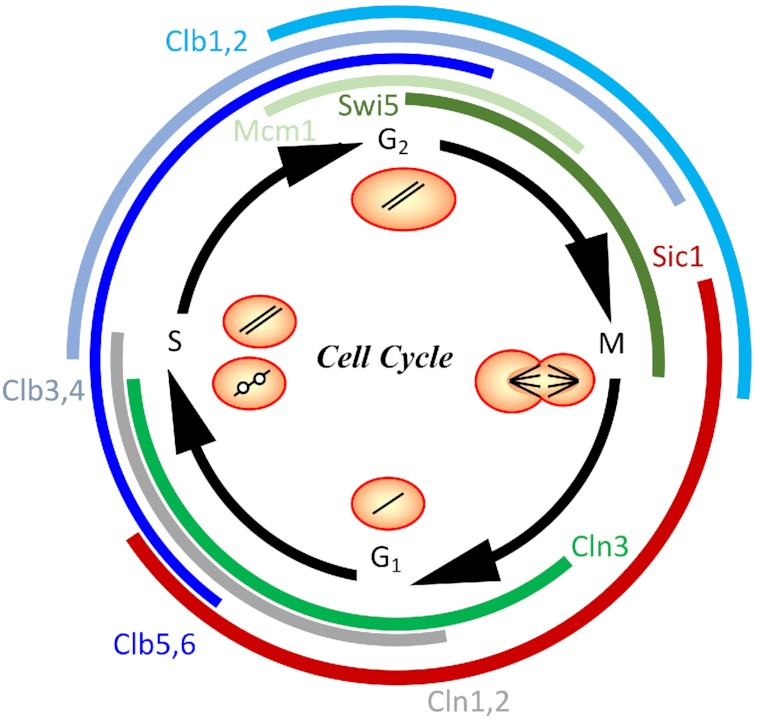
\includegraphics[width=0.9\textwidth]{adlerYeastCellCycle2022_1}
  \caption[
    Overview of the cell division cycle
  ]{
    Overview of the cell division cycle.
    The cell division cycle consists of G\textsubscript{1}, S, G\textsubscript{2}, and M phases (black arrows).
    The cell expresses different cyclins, cell division cycle regulators, as it transitions through different phases of the cell division cycle (coloured curves).
    Adapted from \textcite{adlerYeastCellCycle2022}.}
  \label{fig:intro-cdc-overview}
\end{figure}

% VERY useful citation: adlerYeastCellCycle2022
To demonstrate the definition of biological rhythm, I discuss the cell division cycle, which is well-char\-ac\-terised.
The cell division cycle is a series of cellular events that ensure that a precursor cell divides into two progeny cells.
These events include cell growth and accumulation of biomass, replication of genetic material with proofreading, and dividing the cell into two compartments.
In eukaryotes, the latter event consists of karyokinesis (division of the nucleus) and cytokinesis (division of the cell).
In budding yeast (\textit{Saccharomyces cerevisiae}), the cell division cycle is divided into the G\textsubscript{1}, S, G\textsubscript{2}, and M phases (Fig.\ ~\ref{fig:intro-cdc-overview}).
In the gap phases (G\textsubscript{1} and G\textsubscript{2}), the cell primarily grows and accumulates biomass.
The cell replicates DNA in the S phase and in the M phase it conducts mitosis, in which chromosomes are segregated between the progeny cells.

The cell division cycle is important in unicellular organisms such as budding yeast as it is the mechanism by which the organism reproduces.
Regulation of the cell division cycle is thus important
because the cell must only divide when necessary,
because the cell must have resources available for division before it does so,
because the cell must ensure faithful replication of DNA to prevent deleterious mutations in progeny cells,
and because the cell must ensure that its components are divided equally between its two progeny cells so that its progeny cells can function normally.
The cell division cycle in budding yeast has checkpoints between phases to ensure that biological events from the previous phases are completed before the cell proceeds to the next one.
The most important checkpoint is START in late G\textsubscript{1} phase, at which the cell checks whether it has the resources needed to replicate, and if requirements are met, it irreversibly commits to cell division.
The cell division cycle in budding yeast is also governed by a series of gene regulatory networks that interact in a feedback loop, resulting in oscillatory expression of regulatory proteins, namely, cyclin-CDK complexes that regulate cellular events in a temporal manner \parencite{adlerYeastCellCycle2022, orlandoGlobalControlCellcycle2008, murrayRecyclingCellCycle2004}.
Specifically, cyclins are proteins that sequentially accumulate and are destroyed as the cell transitions through phases of the cell division cycle.
In budding yeast, these cyclins bind to and activate the cyclin-dependent kinase (CDK) Cdc28, which is constitutively expressed.
The different cyclin-CDK combinations in each phase thus determines the events in the cell \parencite{adlerYeastCellCycle2022}:

\begin{enumerate}
  \item In early G\textsubscript{1}, Cln3-Cdc28 phosphorylates Whi5, leading to activation of genes that regulate budding and DNA replication.
  \item In late G\textsubscript{1}, Cln1-Cdc28 and Cln2-Cdc28 hyperphosphorylates Sic1, leading to activation of DNA replication which marks S phase.
  \item In late S phase, Clb1-Cdc28 and Clb2-Cdc28 phosphorylates Ndd1, leading to a feedback loop that activates entry into mitosis.
  \item To exit mitosis, the cell activates a system to target Clb1 and Clb2 for degradation.
\end{enumerate}

To coordinate cell division and metabolism with nutrient availability, budding yeast also has a system of cross-talk between nutrient signalling, growth, and the cell division cycle \parencite{ewaldHowYeastCoordinates2018}.
START is the main control point at which information from nutrient-sensing systems is integrated.
In response to carbon deprivation, Cip1 delays START, and Msa1/2 responds to nutrient depletion and blocks START.
In addition, Rim15 integrates information from TOR and PKA pathways, which respond to nutrient depletion and other stresses, and induces cell division cycle arrest, but also responds to nutrient-poor conditions like non-fermentable carbon sources by inducing an earlier entry into START.
Furthermore, there is also evidence that sudden starvation at other phases affects cell division cycle progression; for example, through the S-phase inhibitor Sic1.
There is also coordination between internal nutrient stores with the cell division cycle.
During S/G\textsubscript{2}/M, Cdc28 activates the trehalase Nth1 so that the storage carbohydrate can be liquidised to provide glucose for glycolysis \parencite{ewaldYeastCyclinDependentKinase2016}.
Additionally, during G\textsubscript{1}/S, Cdc28 activates the lipase Tgl4 to break down storage lipids \parencite{kuratCdk1Cdc28DependentActivation2009}.
There is also evidence for an additional cyclin-dependent kinase, Pho85 \parencite{huangPho85MultifunctionalCyclindependent2007}, which acts to inhibit the expression of genes involved in the phosphate starvation response in high levels of environmental phosphate \parencite{oneillRegulationPHO4Nuclear1996}, and also has roles in inhibiting glycogen synthase \parencite{wilsonSubstrateTargetingYeast1999}.

% [COMMENTED OUT MAIN TEXT -- DOESN'T FIT IN WITH THE REST]
% As with other biological rhythms, the cell division cycle also includes a system to control it, so that DNA replication occurs once every cell division cycle and so that the cell only divides when necessary.
%The importance of such control systems are highlighted by disorders when these systems are impaired, such as chromosome aberrations and cancer (uncontrolled cell division).

\begin{figure}
  \centering
  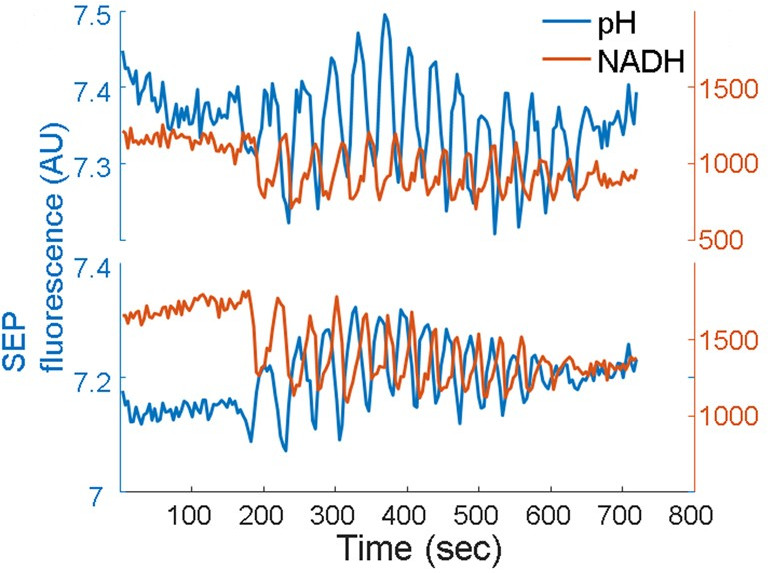
\includegraphics[width=0.9\textwidth]{doddLiveCellImaging2017_3a_adapted}
  \caption[
    Glycolytic cycles
  ]{
    Glycolytic cycles are characterised by oscillations in NADH (orange) and pH (blue) at a period of approximately 40--50 s, and are usually highly damped.
    Adapted from \textcite{doddLiveCellImaging2017a}.}
  \label{fig:intro-glycolytic-overview}
\end{figure}

% TODO : Add glycolytic cycle paragraph
% - Define it.  Steal bits from later sections that discus this cycle, and also refer back to original papers.
% - Why this cycle exists (see discussion of cited papers)
% - How it is regulated & link to definition of a biological rhythm (mention the PFK system thingy)
Glycolytic oscillations are an example of a biological rhythm whose mechanistic basis is relatively poorly characterised.
The glycolytic oscillation is a biochemical oscillator in budding yeast, characterised by damped  oscillations in the levels of glycolytic intermediates at the time scale of 40--50 seconds  \parencite{ghoshOscillationsGlycolyticIntermediates1964}.
These oscillations have been observed as a response to high-glucose conditions and in anaerobic conditions.
Later studies show that levels of NADH \parencite{lloydSaccharomycesCerevisiaeOscillatory2019, olsenOscillationsYeastGlycolysis2021}, pH, and mitochondrial membrane potential \parencite{doddLiveCellImaging2017a} also oscillate at the same frequency (Fig.\ \ref{fig:intro-glycolytic-overview}).
Many hypotheses have been proposed to explain the existence of glycolytic oscillations, but there is no consensus \parencite{lloydSaccharomycesCerevisiaeOscillatory2019}, though \textcite{thokeConstantLowentropyProcess2018} proposed that these oscillations are the result of cells attempting to maintain a constant low-entropy state while remaining metabolically active.
Evidence shows that glycolytic oscillations are regulated through solely biochemical means.
Specifically, a high ADP/ATP ratio and the presence of fructose-1,6-bisphosphate activate the activity of phosphofructokinase, which then controls the flux through glycolysis, forming a negative feedback loop that causes oscillations \parencite{ghoshOscillationsGlycolyticIntermediates1964, higginsChemicalMechanismOscillation1964}.
Such a biochemical mechanism would explain how oscillations are sustained at a short timescale.

\subsubsection{Mathematical basis of biological rhythms}
\label{subsubsec:intro-ymc-biological_rhythms-theoretical_basis}
% - Mathematics of systems of coupled oscillators.

% Single oscillations
% Useful here: cell division cycle modelling literature, e.g. Novak/Tyson,
% Adler et al. (2022) -- comprehensive review of cell division cycle models
% Goldbeter (2022) -- models of several examples
The mathematical modelling of biological rhythms originated in work in the 1960s, which included simple systems of ordinary differential equations to describe negative feedback control circuits \parencite{goodwinOscillatoryBehaviorEnzymatic1965, griffithMathematicsCellularControl1968}.
Experimental observations have then informed the development of models with finer detail.
Furthermore, synthetic genetic circuits have also been modelled and developed \parencite{elowitzSyntheticOscillatoryNetwork2000}.

To illustrate the modelling of a natural biological rhythm, I discuss the cell division cycle.
The well-characterised cell division cycle has inspired models with a variety of approaches.
Early models are based on a negative feedback loop of key components as identified by experimental studies.
For example, \textcite{goldbeterMinimalCascadeModel1991} assumed a minimal model of one cyclin, one kinase, and one protease to construct a negative feedback loop with a delay, giving rise to stable oscillations.
Such a strategy forms the basis of later models that incorporate more detail, including additional control points of the cell division cycle \parencite{chenIntegrativeAnalysisCell2004}, responses to perturbations such as osmotic stress \parencite{adroverTimeDependentQuantitativeMulticomponent2011}, and relationship with other oscillators like the circadian rhythm \parencite{gerardEntrainmentMammalianCell2012, charvinForcedPeriodicExpression2009, droinLowdimensionalDynamicsTwo2019}.
More recent, comprehensive models include \textcite{adlerYeastCellCycle2022} which is based on a system of ordinary differential equations adapted for the modelling to pheromone and osmotic shock responses, and \textcite{novakMitoticKinaseOscillation2022}, which models the cell division cycle as a series of switches between two stable steady states whose behaviour is regulated by the CDK oscillator.

Less well-characterised natural biological rhythms have given rise to models with fewer detail and precision.
An example is glycolytic oscillations.
Most models focus on few intermediates of glycolysis that would explain the observed oscillations.
\textcite{ghoshOscillationsGlycolyticIntermediates1964} proposed a simple biochemical mechanism governed by the action of phosphofructokinase, dependent on the concentration of fructose-1,6-bisphosphate.
\textcite{higginsChemicalMechanismOscillation1964} then tested this mechanism, described by differential equations that model six chemical reactions, computationally.
Later, \textcite{termoniaOscillationsControlFeatures1981} incorporated pyruvate kinase kinetics and levels of AMP, ADP, and ATP as part of their kinetic model based on Michaelis-Menten kinetics.
Other studies focus on non-linear dynamics.
\textcite{goldbeterDissipativeStructuresAllosteric1972} models the product-activated phosphofructokinase reaction, taking into account the allosteric nature of the enzyme.
This model contains a single positive feedback loop as a instability-generating mechanism in a bistability model that explains oscillations.
In \textcite{moranOnsetBirhythmicityRegulated1984}, the model was modified to incorporate a reaction of product recycling into substrate to explain birhythmicity, namely, the potential for oscillations of different amplitudes.
Another development of the model includes a three-variable model that represents two coupled reactions each under a positive feedback loop, explaining more complex oscillatory phenomena that could arise from pulsing of substrates \parencite{decrolyBirhythmicityChaosOther1982}.
In contrast to work that models the cell division cycle, gene expression dynamics and the effects of perturbations have not been incorporated in the modelling of the glycolytic cycle.

% Forced oscillators, coupled oscillators
% Useful here: \textcite{tysonTimekeepingDecisionmakingLiving} and related reviews
As biological rhythms are often coupled with each other, forced and coupled oscillators have been modelled.
If an oscillator is forced, it has a natural oscillation frequency, but is forced from it due to an external force applied at a regular interval.
An example is the circadian clock, which is entrained to the light-dark cycle \parencite{goldbeterMultisynchronizationOtherPatterns}.
Yeast glycolytic oscillations can also be entrained via a periodic input of substrate.
Forced oscillators are closely linked to coupled oscillators, in which two oscillators are coupled to each other by certain activation or deactivation events.
Two coupled oscillators tend to oscillate at a compromise frequency if the natural frequencies of each are close enough to each other.
Otherwise, complex oscillations can occur: the oscillators lock to a rational ratio of frequencies --- i.e.\ one oscillator goes through $p$ periods while the other goes through $q$ periods.
In this case, the exact ratio depends on the ratio of the natural frequencies.
Furthermore, in certain cases, chaos can occur.
There is a mathematical basis in Arnold tongues \parencite{heltbergTaleTwoRhythms2021}.
Experimental observations support this.
For example, \textcite{charvinForcedPeriodicExpression2009} showed that externally forcing cell division cycles via glucose pulsing leads to phase-locking of the cell division cycle oscillator only within a range of extrinsic periods.

The yeast metabolic cycle has been modelled as a system of coupled oscillators \parencite{papagiannakisAutonomousMetabolicOscillations2017,ozsezenInferenceHighLevelInteraction2019}, based on how it is linked to the cell division cycle.
I will discuss this in section \ref{subsec:intro-ymc-model}.

\subsection{Definition and description of the yeast metabolic cycle}
\label{subsec:intro-ymc-definition}
% Worth re-reading: Mellor 2016, Lloyd 2019

The yeast metabolic cycle is an ultradian biological rhythm which has been described to entail oscillations in oxygen consumption, metabolite concentrations, transcript levels, and cellular events, at the population level.
This yeast metabolic cycle is linked to the cell division cycle, but operates autonomously.

The yeast metabolic cycle is classed as a type of biological rhythm because it has the properties that define a biological rhythm.
Namely, it has gene-expression oscillators as evidenced by transcript cycling in its phases,
it has biochemical oscillators as evidenced by changes in dissolved oxygen in the chemostat,
and it has metabolite oscillations as evidenced by changes in the levels of compounds that undergo redox reactions like NADH/NADPH and flavins.

\subsubsection{Phases of the yeast metabolic cycle}
\label{subsubsec:intro-ymc-definition-phases}
% INTEGRATE THIS STRUCTURE IN EACH PARAGRAPH THAT DISCUSSES EACH PHASE
% 1. Overarching theme of phase
% 2. Cellular events (cell division cycle, mitochondria)
% 3. Metabolic events (metabolite concentrations, redox)
% 4. Transcript/genetic events.
% Or any that make sense, e.g. 3 main events and all the evidence from different
% parts of biochemistry.
% Structure should then link well with the definition of biological rhythms in
% a previous subsection.
% ---------------------------------------------------------------------

\begin{figure}
  \centering
  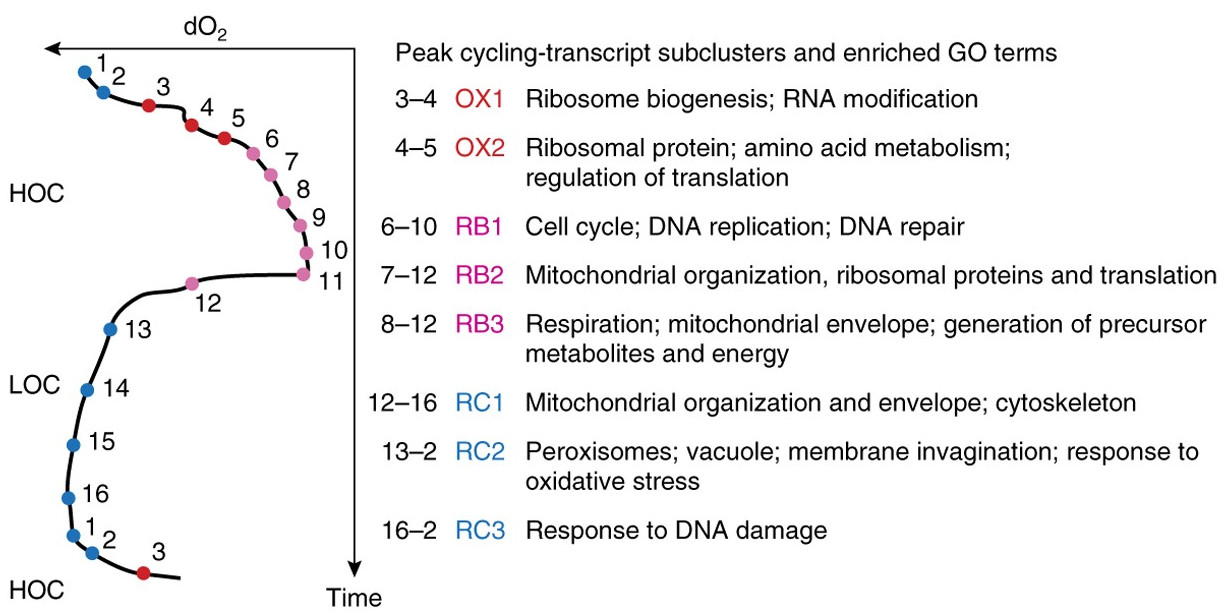
\includegraphics[width=1.0\textwidth]{mellorMolecularBasisMetabolic2016_3c_adapted}
  \caption[
    Phases of the yeast metabolic cycle
  ]{
    Phases of the yeast metabolic cycle,
    with (left) high- (HOC) and low-oxygen consumption (LOC) phases defined by changes in dissolved oxygen concentration (dO\textsubscript{2}) over time in the chemostat
    and (right) oxidative (OX), reductive-building (RB) and reductive-charging (RC) phases defined by cycling of transcripts.
    Adapted from \textcite{mellorMolecularBasisMetabolic2016}.}
  \label{fig:intro-ymc-overview}
\end{figure}

Based on chemostat studies,
the YMC can be divided into two major phases: an oxidative, high-oxygen consumption (OX/HOC) phase and a reductive, low-oxygen consumption (RED/LOC) phase (Fig.\ \ref{fig:intro-ymc-overview}).

\begin{figure}
  \centering
  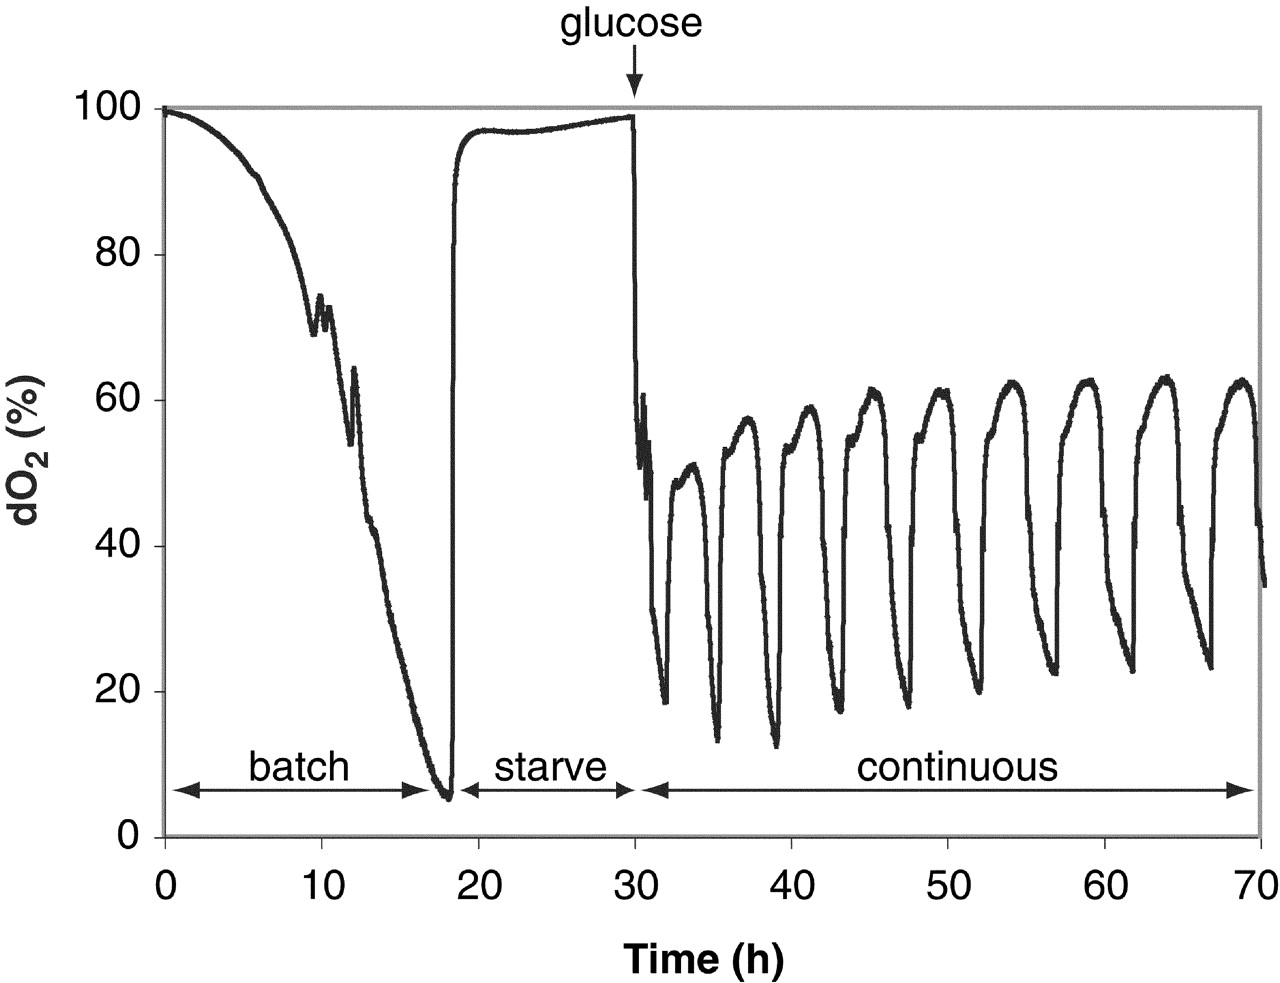
\includegraphics[width=0.9\textwidth]{tuLogicYeastMetabolic2005_1}
  \caption[
    The yeast metabolic cycle has been described as spontaneous respiratory cycles
  ]{
    The yeast metabolic cycle has been described as spontaneous respiratory cycles of 4--5 hours, as evidenced by regular oscillations of dissolved oxygen in the chemostat, after starvation period.
    Adapted from \textcite{tuLogicYeastMetabolic2005}.}
  \label{fig:intro-ymc-tu-oxygen}
\end{figure}

\begin{figure}
  \centering
  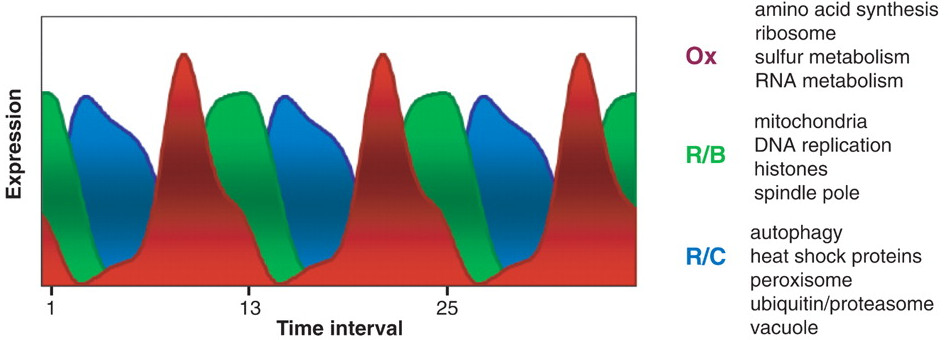
\includegraphics[width=1.0\textwidth]{tuLogicYeastMetabolic2005_3d_adapted}
  \caption[
    The yeast metabolic cycle is characterised by transcript cycling
  ]{
    The yeast metabolic cycle is characterised by transcript cycling.
    Such transcripts are divided into three clusters based on their patterns and phase relationship.
    The peaking of these transcripts correspond to the three (OX, RB, RC) phases of the yeast metabolic cycle.
    Adapted from \textcite{tuLogicYeastMetabolic2005}.}
  \label{fig:intro-ymc-tu-transcripts}
\end{figure}

% Though Lloyd/Murray camp also describe these 3 phases
Many authors \parencite{slavovMetabolicCyclingCell2011, murrayRedoxRegulationRespiring2011, caustonMetabolicRhythmsFramework2018} use oxygen consumption rates, evidenced by the change of dissolved oxygen concentrations over time, as a basis to refer to the YMC as a two-phase cycle (Fig.\ \ref{fig:intro-ymc-tu-oxygen}).
Though, there are authors \parencite{machneYinYangYeast2012} that base their two-phase model on the clustering of transcript level patterns.
\textcite{krishnaMinimalPushPull2018} interpret the oxidative phase as a growth state, while the reductive phase is a quiescent state.
In contrast to the two-phase model, some authors identify a three-phase model with a reductive-building (RB) phase and a reductive-charging (RC) phase within the reductive phase, especially within the long-phase (4--5 hours) yeast metabolic cycle.
This three-phase model is primarily based on cellular events, including clustering of transcript trajectories \parencite{tuLogicYeastMetabolic2005} (Fig.\ \ref{fig:intro-ymc-tu-transcripts}) and of metabolite concentration trajectories \parencite{tuCyclicChangesMetabolic2007}.

\begin{figure}
  \centering
  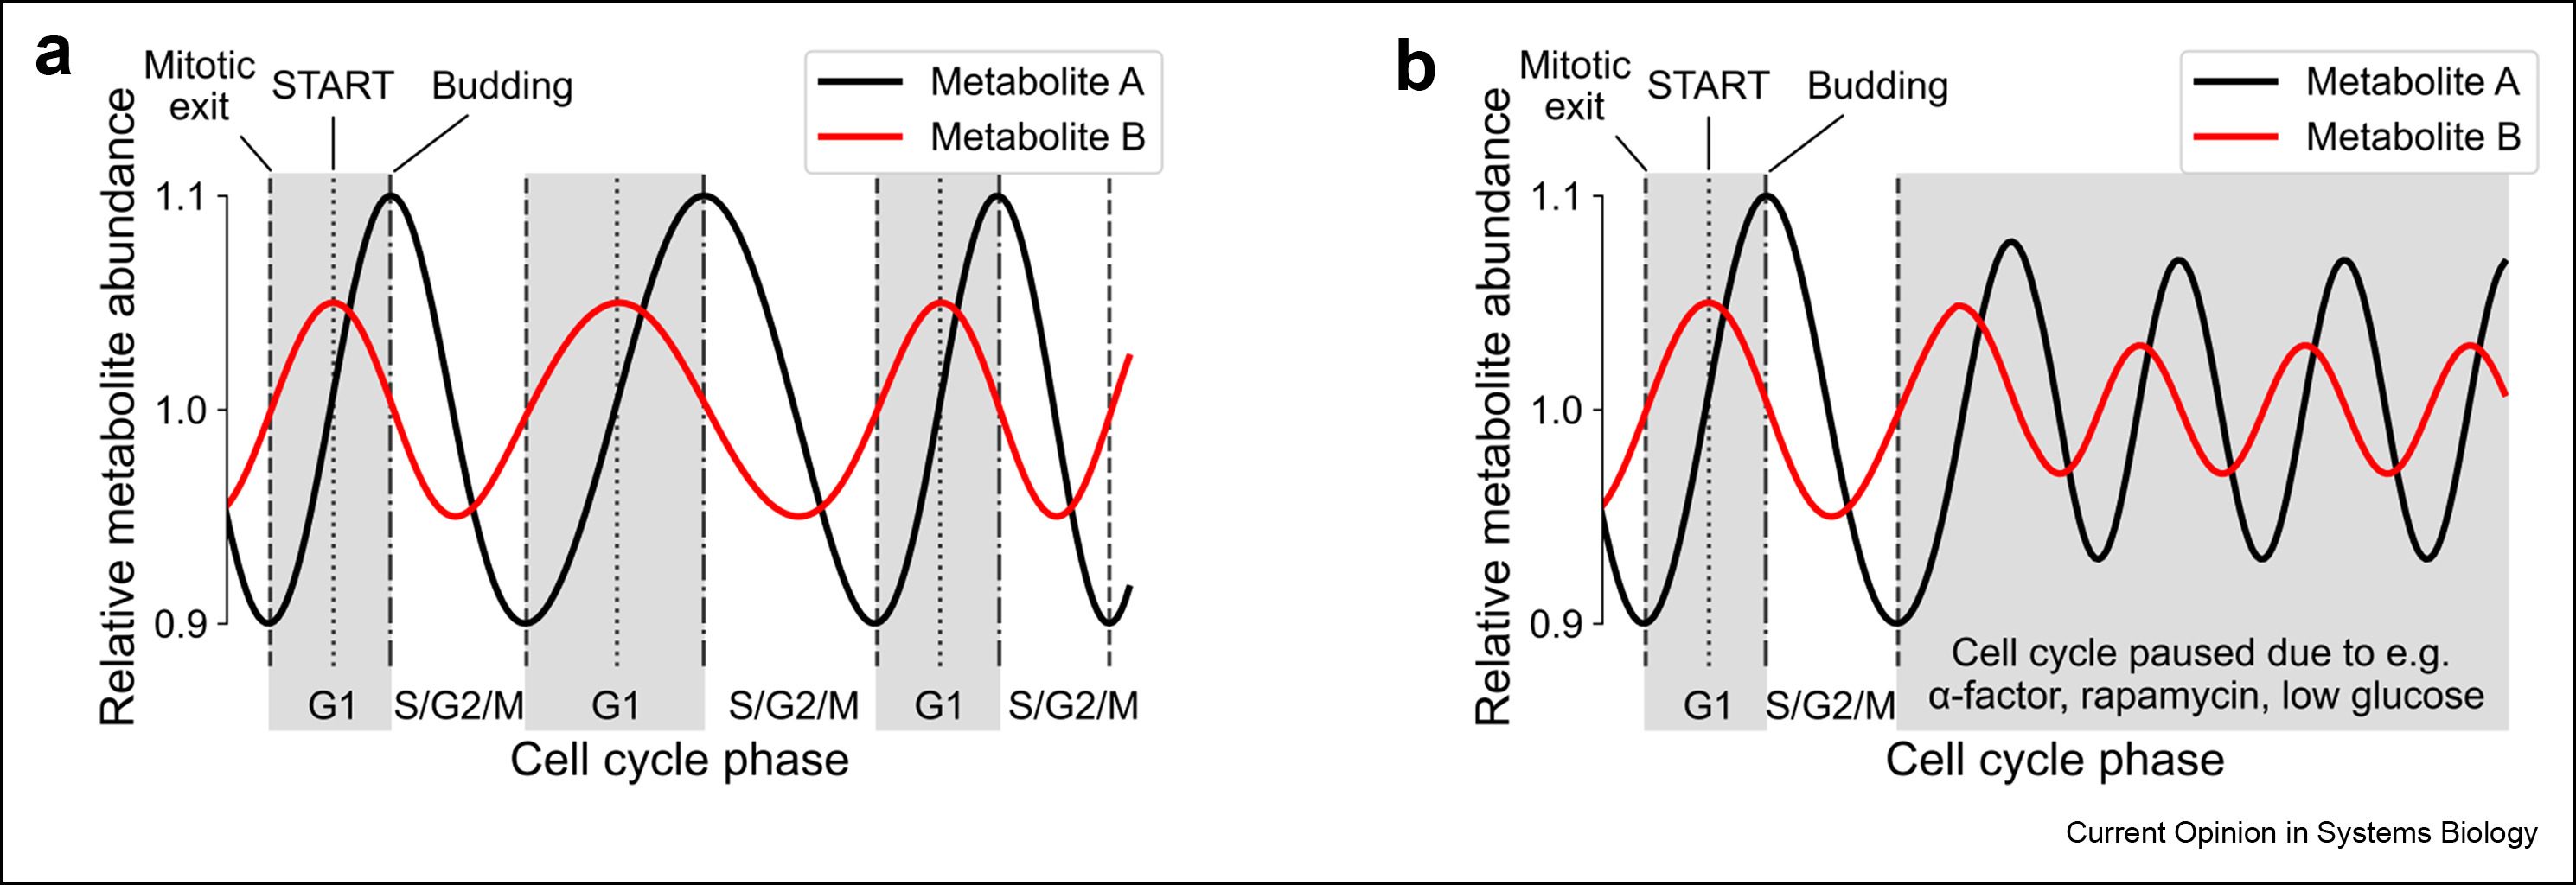
\includegraphics[width=1.0\textwidth]{zylstraMetabolicDynamicsCell2022_1}
  \caption[
    The yeast metabolic cycle seen as coordinated cycling of metabolites in the cell
  ]{
    The yeast metabolic cycle seen as coordinated cycling of metabolites in the cell, generated autonomously of the cell division cycle, but are linked in permissive conditions.
    Adapted from \textcite{zylstraMetabolicDynamicsCell2022}.}
  \label{fig:intro-ymc-overview-ss}
\end{figure}

Single-cell studies \parencite{papagiannakisAutonomousMetabolicOscillations2017, baumgartnerFlavinbasedMetabolicCycles2018} do not discuss phases as the single-cell microfluidic set-up does not allow live monitoring of transcription, and oxygen consumption rate can only be measured from chemostat cultures.
Such studies define the metabolic cycle as autonomous oscillations in metabolite levels in individual cells over time (Fig.\ \ref{fig:intro-ymc-overview-ss}).
In the discussion of later chapters, I adhere to this single-cell definition because I perform a single-cell study of the yeast metabolic cycle.
% ---- I don't think any publication explicitly says this -- it's mostly just Kevin IIRC.  I suggest phrasing it differently, below
%However, others [INSERT CHAIN OF PUBLICATIONS HERE] debate the existence of the reductive-charging phase and argue that this phase is an artefact of cellular adaptation to glucose limitation or feast-and-famine conditions.
Possibly, the two- or three-phase response results from cellular adaptation to glucose limitation in chemostat cultures, and it is unknown whether these dynamics hold true in glucose-rich conditions, which cannot be created in a chemostat \parencite{slavovCouplingGrowthRate2011}.

\begin{figure}
  \centering
  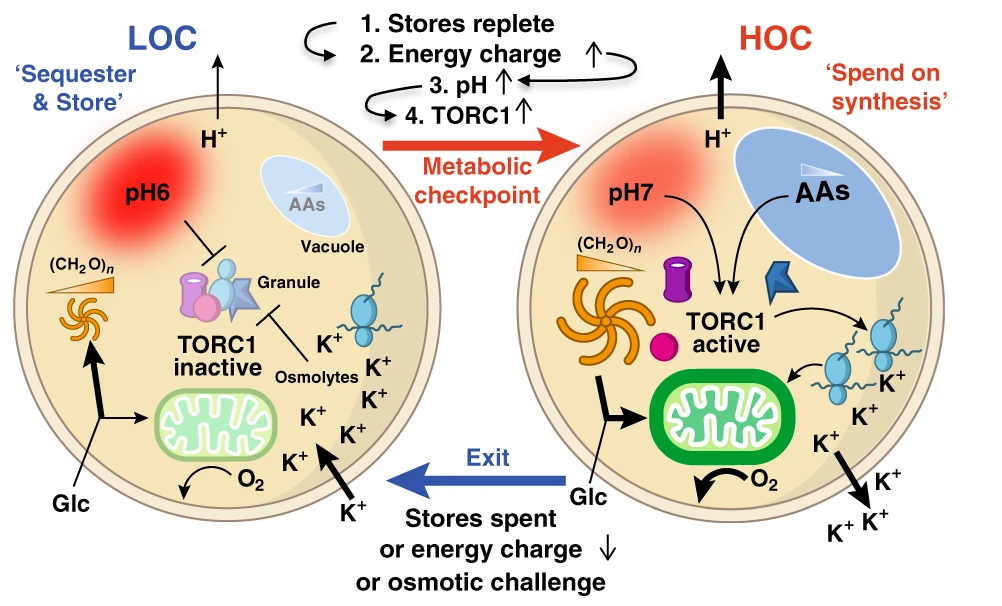
\includegraphics[width=0.9\textwidth]{oneillEukaryoticCellBiology2020_3a_adapted}
  \caption[
    The yeast metabolic cycle seen as temporal partitioning of cellular processes into phases
  ]{
    The yeast metabolic cycle seen as temporal partitioning of cellular processes into phases.
    Here, in the low-oxygen consumption (LOC) phase, the cell accumulate carbohydrates, amino acids, and solutes.
    In contrast, in the high-oxygen consumption (HOC) phase, the reverse is true:
    the cell uses its accumulated resources for biosynthesis and translation.
    Once reserves are exhausted, the cell resumes its LOC phase.
    Adapted from \textcite{oneillEukaryoticCellBiology2020}.}
  \label{fig:intro-ymc-overview-oneill}
\end{figure}

Cellular processes occur in association with the phases of the metabolic cycle (Fig.\ \ref{fig:intro-ymc-overview-oneill}).

In the oxidative phase, cells consume oxygen at a high rate as respiration, fermentation, and
% Potentially may be the reason auxotrophs (hypothetically) don't have YMCs --
% but I showed that they do
energy-demanding processes
like biosynthesis and gene expression occur.
Occurrence of biosynthesis and associated gene expression is confirmed by increased transcripts from genes encoding components of the translation machinery and amino acid biosynthesis \parencite{tuLogicYeastMetabolic2005}.
`Redox state' metabolites, including NADH, NADPH, glutathione \parencite{lloydUltradianMetronomeTimekeeper2005}, and flavins (FMN and FAD)
\parencite{murrayRedoxRegulationRespiring2011} become most oxidised in this phase.
As cells transition from the oxidative to the reductive phase, 70\% of metabolite concentrations peak, at the same time as when NAD(P)H autofluorescence peaks and the DNA synthesis rate is at its maximum \parencite{lloydTemporalArchitectureEukaryotic2006}.

In the reductive phase, cells consume oxygen at a low rate.
During the reductive-building phase, activities linked to mitochondrial growth occur.
In the early reductive-building phase, ethanol and acetate concentrations in the medium peak, marking a transition from oxidative respiration to glycolytic metabolism \parencite{tuCyclicChangesMetabolic2007}.
% as shown here.
There is evidence to suggest that activities linked to cell proliferation --- such as initiation of the cell division cycle, DNA replication, and spindle pole activity --- are gated to the reductive-building phase for both the short-period and long-period YMC.
Such evidence includes budding activity and the pattern of the expression of \textit{YOX1}, which encodes a cell division cycle repressor \parencite{tuLogicYeastMetabolic2005}.

% There are many strings to pull on this phase.
Finally, during the reductive-charging phase,
non-respiratory metabolism and degradation processes occur to prepare the cell for the oxidative phase.
This non-respiratory metabolism includes glycolysis, ethanol and fatty acid metabolism, and nitrogen metabolism.
With these metabolic modes, under the regulation of the transcription factors Msn2p and Msn4p \parencite{kuangMsn2RegulateExpression2017}, acetyl CoA accumulates so ATP can be produced in the oxidative phase \parencite{tuLogicYeastMetabolic2005}.
After acetyl CoA levels reach a threshold, it promotes histone acetylation and thus induces the oxidative phase.
These metabolic pathways also optimise production of NADPH --- based on the induction of \textit{GND2} --- to buffer against oxidative stress in the oxidative phase.
Genes associated with protein degradation, ubiquitinylation, peroxisomes, vacuoles, and the proteosome also peak in the reductive-charging phase.

It has been hypothesised that gating activities linked to cell proliferation to the reductive-building phase
creates a temporal separation between oxidative biochemical processes (in OX) and the cell division cycle.
This temporal separation may prevent reactive oxygen species generated by oxidative process from damaging DNA.
However, measuring DNA content and oxygen consumption in cells grown at different growth rates \parencite{slavovCouplingGrowthRate2011} showed that the S phase of the cell cycle may occur in the oxidative phase if the cells have a slow growth rate.
% Not sure if they changed the growth rate of the cells though -- probably quite difficult
% to do in microfluidics setting.
% Re-phrase it a little to make it more different from Papagiannakis et al.
This may be explained by the YMC gating the early and late cell cycle independently, as evidenced by periodic localisation of the anaphase-promoting complex and mitotic exit activator Cdc14 phosphatase in metaphase-arrested cells \parencite{luPeriodicCyclinCdkActivity2010} and, conversely, the persistence of NAD(P)H cycling upon arresting of the late cell cycle by depletion of Cdc14 \parencite{papagiannakisAutonomousMetabolicOscillations2017}, all observed in single cells.
% What would be the function of such flexible gating?  Seems like community
% has no meaningful consensus yet.  Probably allocation of metabolites.
This evidence indicates that the gating between the YMC and the cell cycle is flexible.
Though there is no meaningful consensus as to the function of such flexible gating,
such gating can be instrumental in the allocation of metabolites to different temporal phases of both cellular oscillators.
% Discuss allocation of metabolites later -- and this can be linked to the modelling chapter of thesis.

\subsubsection{History of evidence for the yeast metabolic cycle}
\label{subsubsec:intro-ymc-definition-history}


Aspects of the YMC have been observed over decades.
\textcite{nosohSYNCHRONIZATIONBUDDINGCYCLE1962} discovered that synchronised \textit{S. cerevisiae} cultures show oscillatory oxygen consumption.
\textcite{kasparvonmeyenburgEnergeticsBuddingCycle1969} showed that gas metabolism and energy generation increase upon budding, while \textcite{mochanRespiratoryOscillationsAdapting1973} described a high-amplitude respiratory oscillation following a substrate shift from glucose to ethanol.
\textcite{satroutdinovOscillatoryMetabolismSaccharomyces1992} were the first to describe the metabolic components of a 40-minute YMC for cells in continuous culture.
\textcite{tuLogicYeastMetabolic2005}
first incorporated transcript cycling in the description of the YMC and defined the YMC events,
based on a chemostat-based investigation of growth of budding yeast on glucose-starved conditions.

The yeast metabolic cycle is longer in duration and is more robust than a similar biological oscillator, the glycolytic oscillation.
The glycolytic oscillation has a period on the scale of 40 seconds \parencite{olsenRegulationGlycolyticOscillations2009}.
In contrast, the yeast metabolic cycle has been described, using various definitions, to either exhibit a 40-minute short-phase cycle \parencite{lloydUltradianMetronomeTimekeeper2005, liRapidGenomescaleResponse2006, lloydRedoxRhythmicityClocks2007}, or a long-phase cycle, which is most commonly described to be 4--5 hours \parencite{tuLogicYeastMetabolic2005, tuCyclicChangesMetabolic2007}, but also ranges between 1.4 hours to 14 hours, depending on the chemostat dilution rate \parencite{beuseEffectDilutionRate1998}.

Glycolytic oscillations are highly damped, but yeast metabolic oscillations are robust, lasting for weeks \parencite{lloydRedoxRhythmicityClocks2007}.
Additionally, glycolytic oscillations have been observed in anaerobic conditions \parencite{lloydSaccharomycesCerevisiaeOscillatory2019}, but yeast metabolic cycles have been observed in aerobic conditions.
Moreover, glycolytic oscillations are characterised by fluctuations in NADH fluorescence and glycolytic intermediates.
However, yeast metabolic cycles consist of fluctuations in NADH fluorescence, flavin fluorescence, and ATP concentrations as well as biosynthetic intermediates in TCA cycle, amino acid, and nucleic acid metabolism \parencite{tuCyclicChangesMetabolic2007}.


\subsection{Yeast metabolic cycles under perturbations}
\label{subsec:intro-ymc-perturbations}
% - Nutrient perturbations
  % - Changing concentration or compositions of carbon sources.
  % - Changing concentration or compositions of nitrogen sources.
  % - Key deletion strains shed light on mechanism

Perturbations in growth conditions can affect the length of the metabolic cycle and its relationship with other cellular events.
The long-phase cycle may vary from 1.4 to 14 hours \parencite{caustonMetabolicRhythmsFramework2018}.
The main nutrient perturbations that have been studied are perturbations in carbon sources and in nitrogen sources.

\subsubsection{Perturbations in growth conditions}
\label{subsubsec:intro-ymc-perturbations-nutrient}


Perturbations in carbon sources are well-documented.
% change glucose concentration
Lower glucose concentrations prolong the metabolic cycle, as evidenced by both chemostat studies that assess the effect of changing the dilution rate \parencite{burnettiCellCycleStart2016, oneillEukaryoticCellBiology2020} and by single-cell studies that assess the effect of glucose concentrations in the limiting region \parencite{papagiannakisAutonomousMetabolicOscillations2017}.
% 20 g/L --> 0.5 g/L doesn't seem to significantly prolong it, but maybe
% a greater effect will be seen if we get to the region of glucose limitation
% Though I am aware that this is my experimental observations -- need to see if literature confirms.
For example, decreasing the dilution rate decreases the growth rate, and in turn increases the duration of the oxidative phase relative to the reductive phases \parencite{slavovCouplingGrowthRate2011}, thus prolonging the metabolic cycle.
This effect is pronounced in the region of glucose limitation.
Increasing the glucose concentration beyond a certain point does not produce an effect.
Additionally, several studies \parencite{slavovCouplingGrowthRate2011,oneillEukaryoticCellBiology2020} show that the duration of the low oxygen consumption phase increases while the duration of the high oxygen consumption phase holds constant if the metabolic cycle duration increases due to these reasons.

Such experimental observations could by explained by models such as \textcite{jonesCyberneticModelGrowth1999}, which suggest that as the dilution rate is decreased, metabolic oscillations acquire greater amplitudes and longer periods, but if it is low enough, metabolism becomes entirely oxidative, and metabolic oscillations disappear.
% ferm vs non-ferm
However, non-fermentable carbon sources like pyruvate give long-duration metabolic cycles in single cells, comparable to cells under limiting levels of glucose \parencite{papagiannakisAutonomousMetabolicOscillations2017}.

% bulk addition and depletion
In addition, bulk depletion or addition of a carbon source can reset the phase of the YMC.
%Chemostat studies show that an initial starvation phase is needed to generate long-lasting synchronous metabolic cycles \parencite{tuLogicYeastMetabolic2005}. %[OTHER CITATIONS PROBABLY USEFUL].
%On the other hand,
Adding a bulk carbon source such as acetate, ethanol, or acetaldehyde can reset the phase of the YMC \parencite{kuangMsn2RegulateExpression2017, krishnaMinimalPushPull2018} or eliminate it \parencite{jonesCyberneticModelGrowth1999}.

Perturbations in nitrogen sources are less well-studied.
% Maybe also because long OX stage as it's the stage for biomass building
\textcite{baumgartnerFlavinbasedMetabolicCycles2018}, based on single-cell observations, suggest that decreasing nitrogen source concentration prolongs the YMC, as evidenced by longer flavin oscillations when cells are grown on lower concentrations of yeast nitrogen base (YNB) media or on urea, a non-preferred nitrogen source.

In addition, perturbations outside nutrient sources also affect the YMC.
For example, externally applied hydrogen peroxide, as a source of oxidative stress, shifts the YMC to the oxidative phase \parencite{amponsahPeroxiredoxinsCoupleMetabolism2021}.
% [MOVED FROM PREVIOUS SECTION]
The oscillation period is insensitive to temperatures from \SI{25}{\celsius} to \SI{35}{\celsius} and media pH values from
2.9 to 6.0 \parencite{lloydUltradianMetronomeTimekeeper2005} --- though the period of dissolved-oxygen oscillations decrease as pH decreases to below 2.9 and the oscillations disappear when conditions are too acidic \parencite{oneillEukaryoticCellBiology2020}.
Additionally, the dissolved-oxygen oscillations are robust to media potassium ion concentrations varying between 1 and 10 mM, but disappear when the potassium concentration falls below 1 mM \parencite{oneillEukaryoticCellBiology2020}.

Finally, the phase difference between the YMC and cell cycle varies in different conditions % how?
% Confirmation that the YMC responds to nutrient availability?  How does phase
% resetting help the Cell Division Cycle then?
\parencite{ewaldYeastCyclinDependentKinase2016}. % ok, but have I seen this phase shift with the different media (i.e. SC vs SM)?  What did Ewald have to say about this phase shift??
% 'bulk carbon source' -- could be adaptation to changing nutrient concentrations in general?
%Furthermore, the YMC can oscillate multiple times per cell cycle, or even disappear in some conditions \parencite{baumgartnerFlavinbasedMetabolicCycles2018}. % which conditions?  can these be tested?
% --> also see Causton et al. (2015)
% -----------------------------------------------------------------------------------------------

\subsubsection{Genetic perturbations}
\label{subsubsec:intro-ymc-perturbations-genetic}

\begin{figure}
  \centering
  \begin{subfigure}[htpb]{0.9\textwidth}
   \centering
   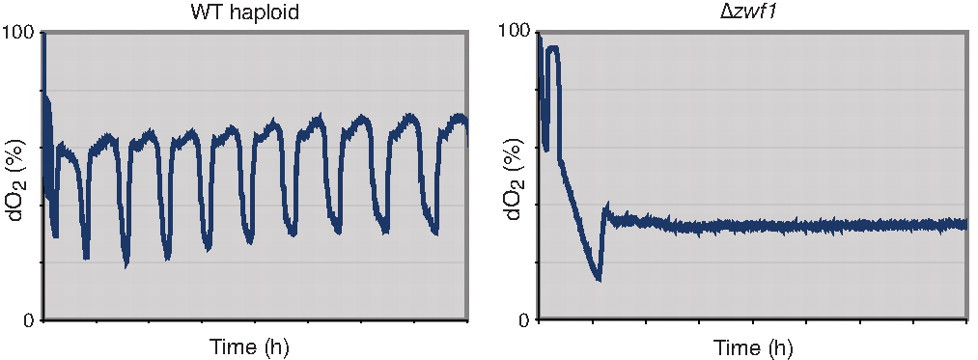
\includegraphics[width=\textwidth]{tuCyclicChangesMetabolic2007_2c_adapted}
   \caption{
   }
   \label{fig:intro-ymc-zwf1}
  \end{subfigure}
  \begin{subfigure}[htpb]{0.4\textwidth}
   \centering
   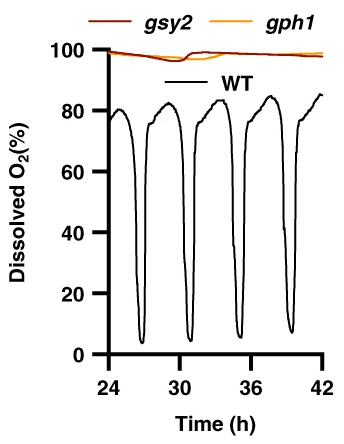
\includegraphics[width=\textwidth]{oneillEukaryoticCellBiology2020_5a_adapted}
   \caption{
   }
   \label{fig:intro-ymc-gsy2-gph1}
  \end{subfigure}
  \begin{subfigure}[htpb]{0.4\textwidth}
   \centering
   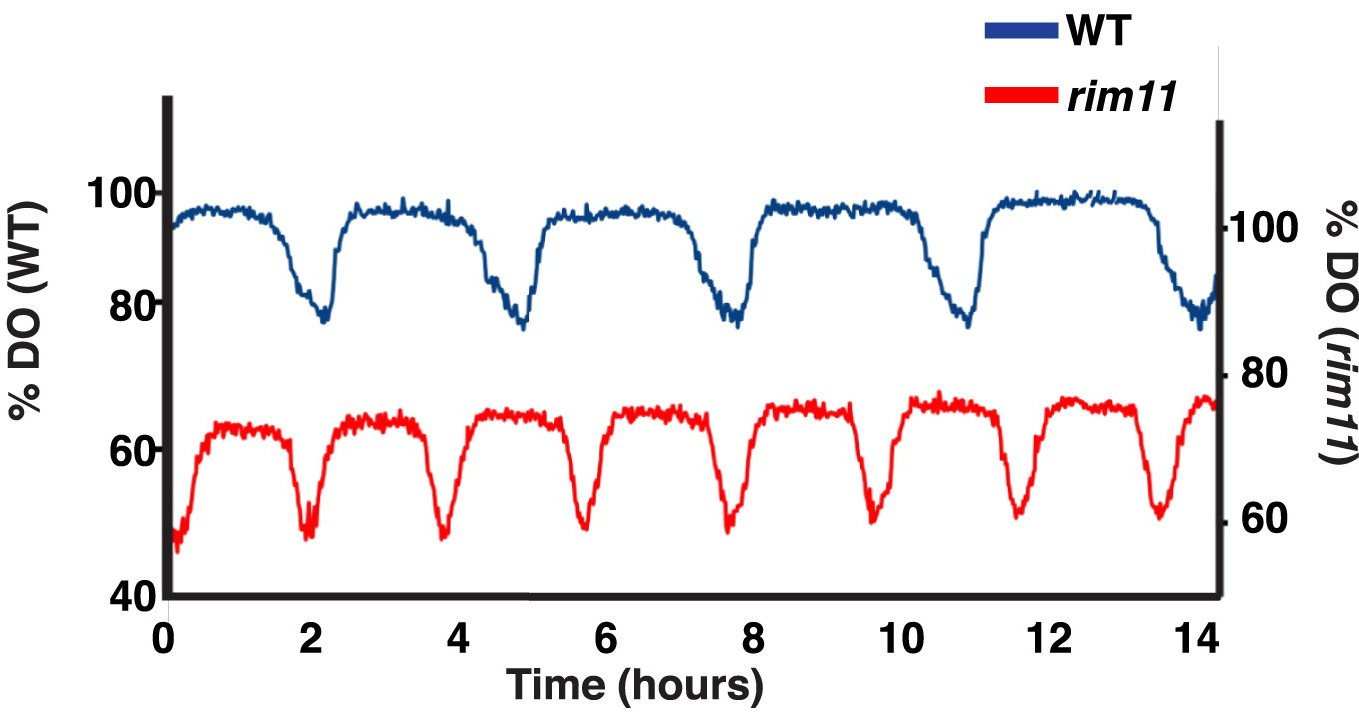
\includegraphics[width=\textwidth]{caustonMetabolicCyclesYeast2015_2e_adapted}
   \caption{
   }
   \label{fig:intro-ymc-rim11}
  \end{subfigure}
  \begin{subfigure}[htpb]{0.4\textwidth}
   \centering
   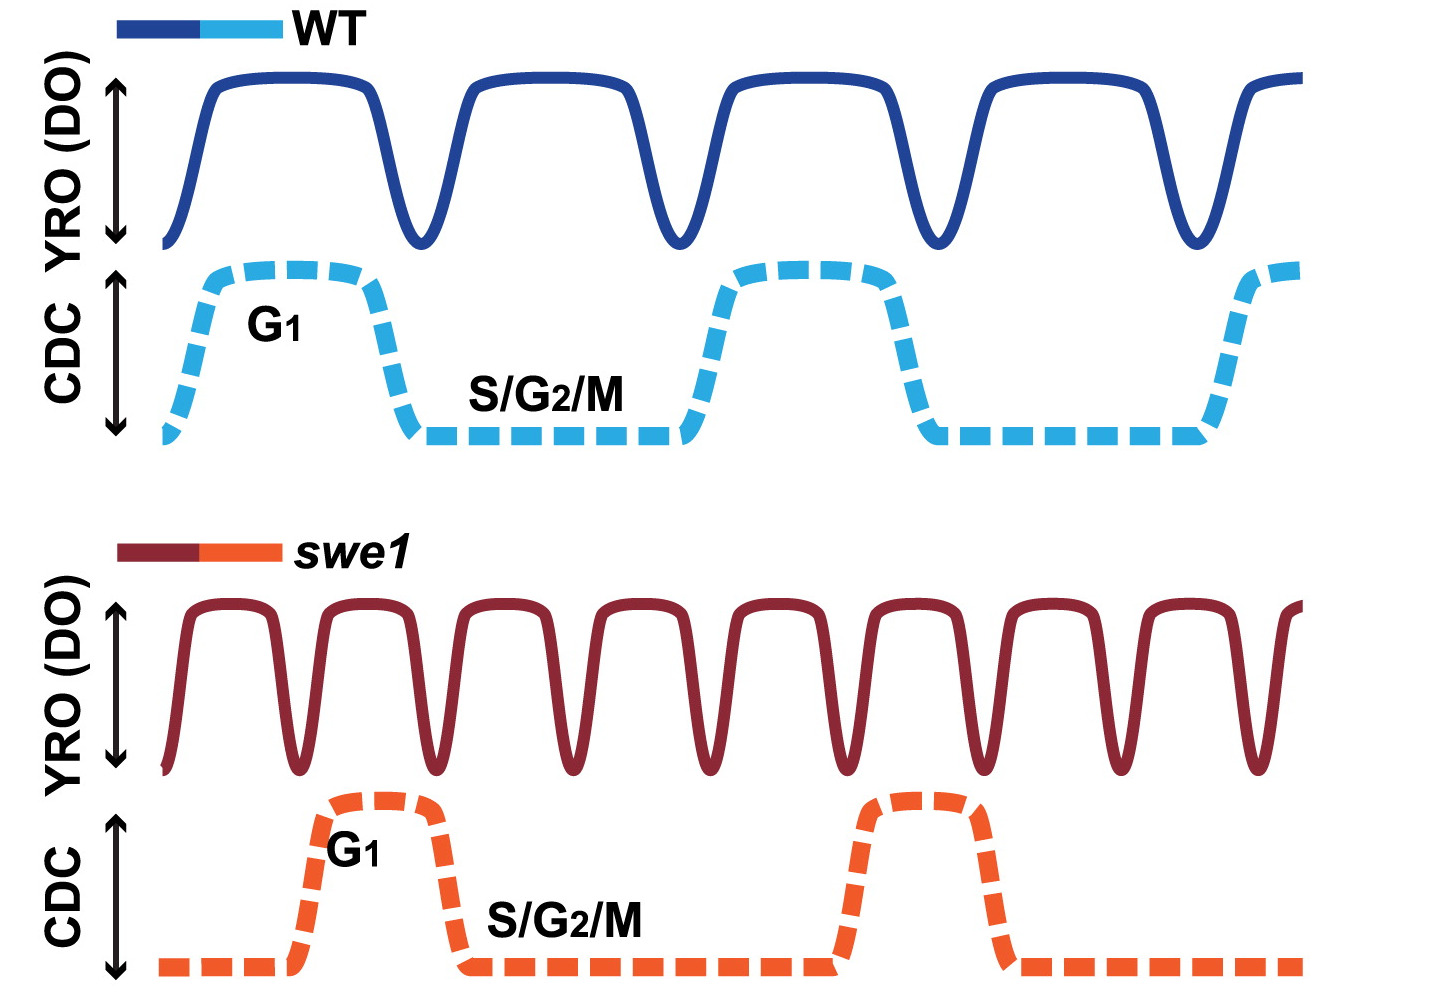
\includegraphics[width=\textwidth]{caustonMetabolicCyclesYeast2015_1e_adapted}
   \caption{
   }
   \label{fig:intro-ymc-swe1}
  \end{subfigure}
  \begin{subfigure}[htpb]{0.4\textwidth}
   \centering
   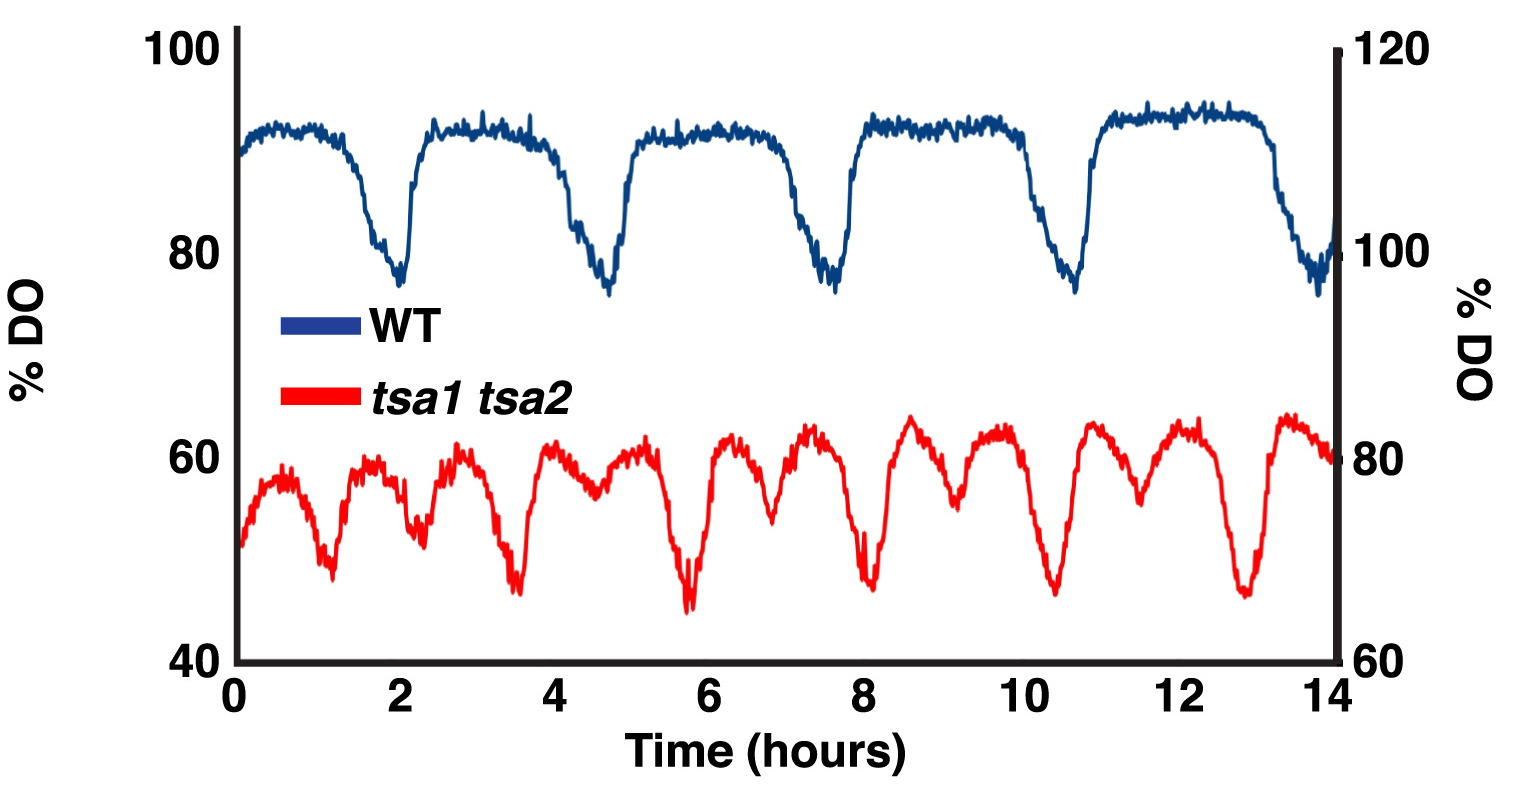
\includegraphics[width=\textwidth]{caustonMetabolicCyclesYeast2015_4a_adapted}
   \caption{
   }
   \label{fig:intro-ymc-tsa1-tsa2}
  \end{subfigure}
  \caption[
    Effect of genetic perturbations on the yeast metabolic cycle
  ]{
    Effect of genetic perturbations on the yeast metabolic cycle, as evidenced by the dissolved oxygen cycles of deletion strains observed in the chemostat.
    %
    \textbf{(\ref{fig:intro-ymc-zwf1})}
    \textit{zwf1$\Delta$} shows no dissolved oxygen cycles.
    Adapted from \textcite{tuCyclicChangesMetabolic2007}.
    %
    \textbf{(\ref{fig:intro-ymc-gsy2-gph1})}
    \textit{gsy2$\Delta$} and \textit{gph1$\Delta$} show no dissolved oxygen cycles.
    Adapted from \textcite{oneillEukaryoticCellBiology2020}.
    %
    \textbf{(\ref{fig:intro-ymc-rim11})}
    \textit{rim11$\Delta$} shows shorter dissolved oxygen cycles.
    Adapted from \textcite{caustonMetabolicCyclesYeast2015}.
    %
    \textbf{(\ref{fig:intro-ymc-swe1})}
    \textit{swe1$\Delta$} shows shorter dissolved oxygen cycles and a modified coupling ratio between the metabolic and cell division cycle oscillators.
    Adapted from \textcite{caustonMetabolicCyclesYeast2015}.
    %
    \textbf{(\ref{fig:intro-ymc-tsa1-tsa2})}
    \textit{tsa1$\Delta$ tsa2$\Delta$} shows dissolved oxygen cycles of a different shape.
    Adapted from \textcite{caustonMetabolicCyclesYeast2015}.
  }
  \label{fig:intro-ymc-del}
\end{figure}

Although the molecular basis of the yeast metabolic cycle is not well-characterised, gene deletions shed light on it.
% Mellor (2016) provide an awesome table.
Genes that control the cell division cycle and metabolism have been deleted in studies.

Several deletions have been shown to remove the metabolic oscillations in chemostats: \textit{zwf1$\Delta$} \parencite{tuCyclicChangesMetabolic2007}, \textit{gsy2$\Delta$}, and \textit{gph1$\Delta$} \parencite{oneillEukaryoticCellBiology2020} (Figs.\ \ref{fig:intro-ymc-zwf1},~\ref{fig:intro-ymc-gsy2-gph1}).

\textit{ZWF1} codes for glucose-6-phosphate dehydrogenase and is thus responsible for entry into the pentose phosphate pathway and subsequently a major source of NADPH generation, so deleting this gene may impair control of cellular redox.
However, because of its role, this gene deletion impairs adapting to oxidative and pH stress and also causes methionine auxotrophy, so it may be difficult to draw conclusions from this deletion in particular.
Furthermore, other enzyme-catalysed reactions in the cell that generate NADPH exist (Idp2p, Ald6p) and have shown to compensate for the loss of \textit{ZWF1} when cells are grown on lactate plates or on liquid cultures with glucose as the carbon source \parencite{minardSourcesNADPHYeast2005}.
This therefore raises the question of just how important \textit{ZWF1} is to the yeast metabolic cycle, and to what extent is NADPH generation needed for control of cellular redox.

On the other hand, \textit{GSY2} and \textit{GPH1} both have roles in glucose/glycogen mobilisation and storage.
The absence of dissolved oxygen cycles in the associated deletions thus suggest that cycling of carbohydrate stores may be needed for the function of the metabolic cycle.
However, metabolic oscillations have been observed in high-glucose conditions \parencite{papagiannakisAutonomousMetabolicOscillations2017, baumgartnerFlavinbasedMetabolicCycles2018} in which glycogen synthesis is repressed, therefore suggesting that glycogen cycling may play a more minor role in defining the yeast metabolic cycle and another nutrient cycling phenomenon may be more responsible.

In addition, \textit{MSN2} and \textit{MSN4} have been shown to regulate acetyl CoA accumulation in the reductive-charging phase, as evidenced by the lack of YMCs in deletion strains \parencite{kuangMsn2RegulateExpression2017}.
This tells us that genes involved in signalling pathways play an important role in the integrity of the metabolic cycle too.

Additionally, other deletions have been shown to change the frequency or shape of dissolved oxygen cycles.
\textcite{caustonMetabolicCyclesYeast2015} provide several examples, of which I discuss \textit{rim11$\Delta$}, \textit{swe1$\Delta$}, and \textit{tsa1$\Delta$ tsa2$\Delta$}. % they actually had more, but these are the three that pop in my head right now

Rim11p is the yeast homolog of the GSK3$\beta$ serine/threonine kinase, which regulates metabolism and plays a role in setting the speed of the circadian clock.
The \textit{RIM11} deletion has been shown to give shortened periods of dissolved-oxygen metabolic cycles in the chemostat, thus pointing towards a common mechanism for both biological oscillators (Fig.\ \ref{fig:intro-ymc-rim11}).

Swe1p is a conserved cell division cycle regulator that functions at the G2/M checkpoint and has roles in coupling the cell division cycle with the circadian rhythm.
Deleting \textit{SWE1} also resulted in shortened periods of dissolved-oxygen metabolic cycles but with the same rate of DNA replication, suggesting a dysregulation in the coupling between the yeast metabolic cycle and the cell division cycle (Fig.\ \ref{fig:intro-ymc-swe1}).

Tsa1p and Tsa2p are paralogous cytoplasmic thioredoxin peroxidases that cooperate in the peroxiredoxin-thioredoxin system to eliminate reactive oxygen species and have been shown to be a marker for circadian rhythms.
A double deletion of the two associated genes still results in metabolic cycles, but with an additional burst in high oxygen consumption during what would otherwise be the reductive-charging phase, showing that the peroxiredoxin-thioredoxin system is instrumental in the integrity of the yeast metabolic cycle (Fig.\ \ref{fig:intro-ymc-tsa1-tsa2}).
In addition, \textcite{amponsahPeroxiredoxinsCoupleMetabolism2021} show the presence of cycling peroxiredoxin oxidation during the YMC using chemostat-based studies, with a corresponding cycling of hydrogen peroxide.
They also confirm that inactivating peroxiredoxins --- \textit{tsa1$\Delta$ tsa2$\Delta$}, additionally with inducible degradation of Ahp1, another cytosolic peroxiredoxin --- disrupts the metabolic cycle and decouples it from the cell division cycle.

%Moreover, deletion of \textit{GTS1} shortens the oscillation periods \parencite{lloydUltradianMetronomeTimekeeper2005},
Taken together, these deletion studies show that regulators of other biological rhythms and of redox metabolism play a role in the regulation of the YMC.

However, few genetic perturbation studies have been attempted in single-cell studies.
The most significant is in \textcite{baumgartnerFlavinbasedMetabolicCycles2018}, in which by deleting genes (\textit{atp5$\Delta$}, \textit{cyt1$\Delta$}) required for respiration, they showed that metabolic cycling does not require respiration.

\subsection{Modelling the yeast metabolic cycle}
\label{subsec:intro-ymc-model}

%[THE SUMMARY FIGURES FROM THESE PAPERS MAY BE USEFUL TO HELP ILLUSTRATE THE IDEAS]

Mathematical models have been developed to explain the aspects of the YMC.
An early model is \textcite{jonesCyberneticModelGrowth1999} which simulates dynamic competition between three modes of metabolism --- fermentation, glucose oxidation, and ethanol oxidation --- using differential equations.
This model predicts spontaneous generation of oscillations in dissolved oxygen, cell mass, and storage carbohydrates in continuous cultures.
This prediction is consistent with chemostat-based studies of the yeast metabolic cycle.
Furthermore, the model predicts that, within a window of dilution rate values, if the dilution rate decreases, the dissolved oxygen oscillations increase in amplitude and period.
The increase in period agrees with experimental studies such as \textcite{oneillEukaryoticCellBiology2020}.
However, the model also predicts oscillations in the extracellular concentrations of glucose and ethanol.
In theory, such oscillations can only occur if there is a nutrient-consuming prey species that is in turn consumed by two competing predators, or if there are two competitors and an inhibitor added to the chemostat that inhibits only one of the competitors \parencite{smithTheoryChemostatDynamics1995}. % discuss whether the J & K model fits the latter case only if someone complains about it.

\textcite{krishnaMinimalPushPull2018} use a frustrated bistability model to describe a relaxation oscillator that explains how a population of yeast cells switches between quiescent and growth states when faced with a limited amount of metabolic resources.
This model assumes that the cells retain hysteresis of their current state and posits that cells of two populations communicate through diffused acetyl-CoA to sustain population-level oscillatory behaviour.
\textcite{burnettiCellCycleStart2016} also propose that yeast cells committed to the metabolic cycle secrete metabolites that induce other cells to enter the metabolic cycle, provided that they have enough storage carbohydrates.
Taken together, the models provide an attractive cell-to-cell signalling explanation for the population-level behaviour observed in the chemostat.
However, such an explanation does not explain the presence of metabolic cycling in single-cell conditions in which cells are physically separated and thus signalling between cells cannot occur --- though it must be noted that autonomous generation of metabolic cycles and synchrony of metabolic cycles in a population can each arise from mechanisms that are independent of each other.

\begin{figure}
  \centering
  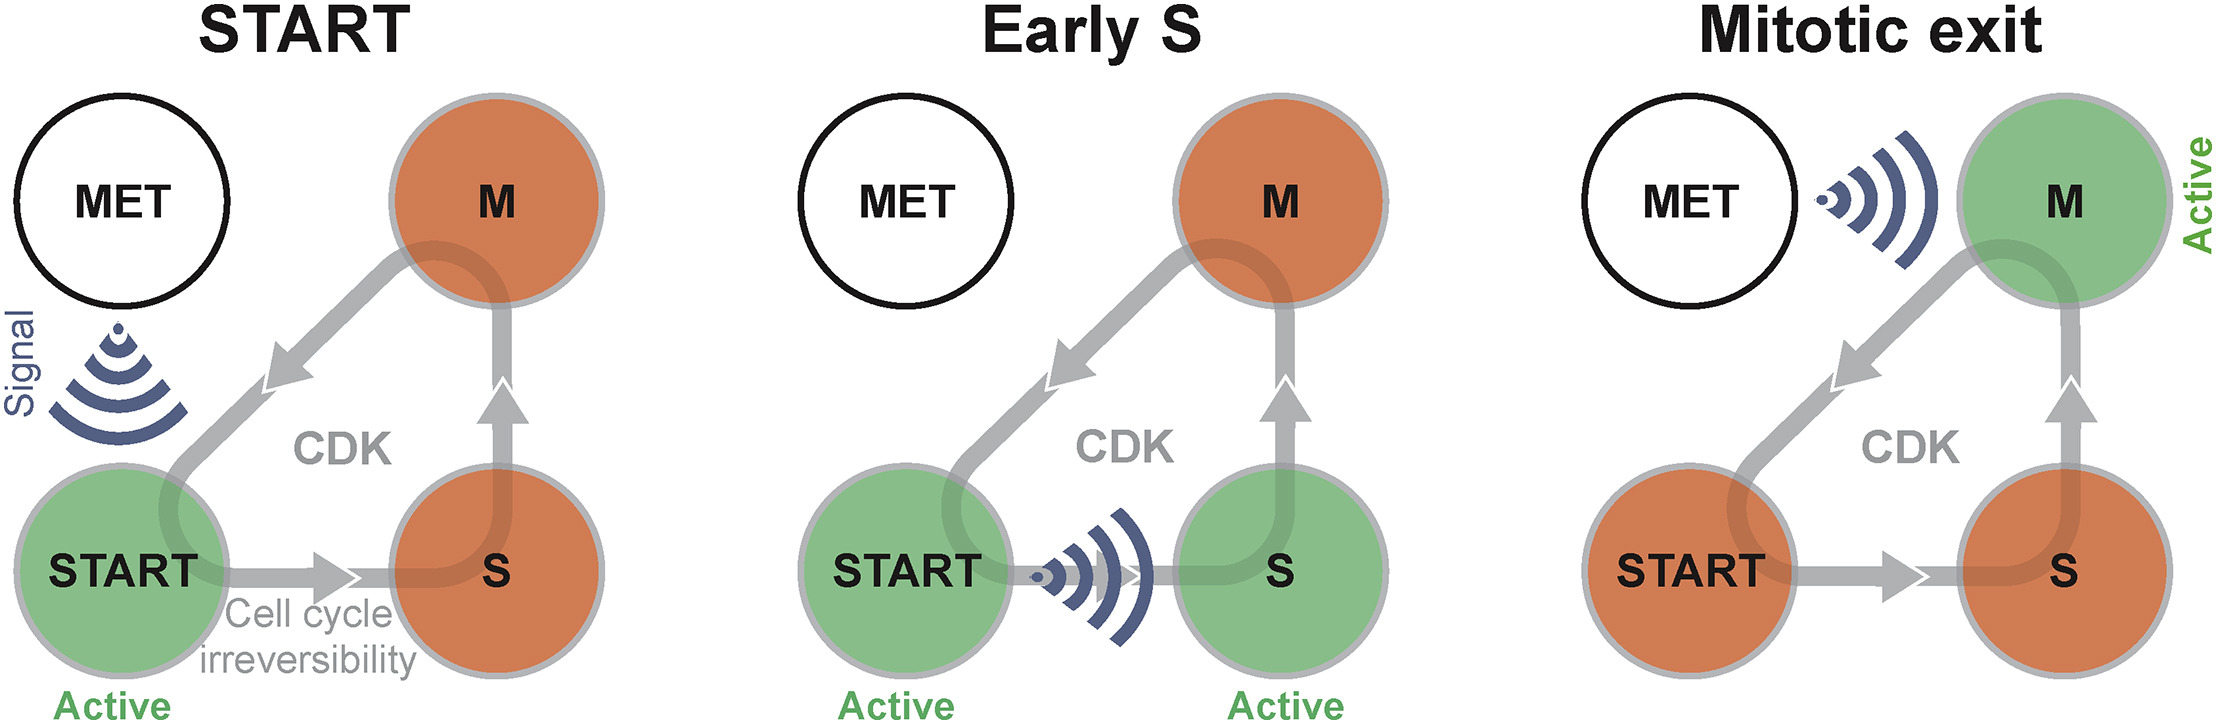
\includegraphics[width=1.0\textwidth]{ozsezenInferenceHighLevelInteraction2019_7}
  \caption[
    The relationship between the yeast metabolic cycle and the cell division cycle can be seen as a system of coupled oscillators
  ]{
    The relationship between the yeast metabolic cycle and the cell division cycle can be seen as a system of coupled oscillators.
    Namely, the cell division cycle is modelled as three oscillators (START, S, M), and the yeast metabolic oscillator (MET) gates entry into START and M phases, while progression from START to S is independent of the metabolic cycle.
    Adapted from \textcite{ozsezenInferenceHighLevelInteraction2019}.}
  \label{fig:intro-ymc-coupled_oscillators}
\end{figure}

Based on single-cell experimental observations, \textcite{ozsezenInferenceHighLevelInteraction2019} use a deterministic Kuramoto model to explain the interaction between one metabolic oscillator and three cell cycle oscillators at different stages.
This study builds upon use of the Kuramoto model to model collective oscillatory behaviour in other biological systems.
The study uses growth on different carbon source conditions to determine parameters that define the natural frequencies of the cell division cycle oscillators and the strength of the coupling between the four oscillators.
Parameter optimisation predicts that the metabolic cycle most strongly influences the START point of the cell division cycle, and more weakly influences the M and S phases, while the three points of the cell division cycle negligibly influence each other (Fig.\ \ref{fig:intro-ymc-coupled_oscillators}).
Under perturbations, the model system also exhibits stability but also a shift in oscillation frequency, agreeing with experimental observations, and also predicts the effects of Cdc20 and Cdc14 dynamic depletions.
However, a key criticism of this model-based study is that by using the Kuramoto model, it makes simplistic assumptions about the oscillators, which may be unrealistic especially given how little is known about the mechanistic basis of the metabolic oscillator.

% [This is a bit out of place... probably nix it given that I've given up on using this.]
% Additionally, a data-driven stochastic modelling approach was used to describe the relationship between the circadian and cell cycle oscillators without assuming a prior relationship \parencite{droin_low-dimensional_2019}.
% This strategy is yet to be applied to the metabolic and cell cycle oscillators.
% However, \textcite{ozsezenInferenceHighLevelInteraction2019} assumed the same, specific coupling function for all interactions between the four oscillators.

Taken together, modelling approaches have been able to predict some aspects of the metabolic cycle.
But, most focus on specific aspects to the detriment of other experimental observations, and none sufficiently reconcile observations from both chemostat-based and single-cell studies.
Constructing more accurate models is complicated by how little of the mechanistic basis of the yeast metabolic cycle has been elucidated thus far.

\subsection[Big picture/Hypothesis]{Big picture/Hypothesis: a nutrient sensor than entrains the cell division cycle?}
\label{subsec:intro-ymc-hypothesis}

From existing evidence, we can create a big picture of the yeast metabolic cycle.
The yeast metabolic cycle is a autonomous biological oscillator that operates at a range of frequencies in response to a range of (permissive) growth conditions, as evidenced by how extreme conditions impair the oscillator.
Based on chemostat-based studies, such extreme conditions include poor nutrient quality, media being too acidic, and potassium ion concentration being too low.
However, there is reason to believe that the metabolic oscillator can function in some conditions previously deemed to be unfavourable.
For example, single-cell studies show that yeast cells show metabolic oscillations in high-glucose conditions.
Within the permissive growth conditions, different conditions affect the frequency of the metabolic cycle.
For example, a low concentration of glucose or nitrogen source results in longer cycles, and bulk addition of certain compounds can reset the phase of the metabolic cycle.
These observations support the idea that the metabolic oscillator includes the functionality of a nutrient sensor.

The observations suggest that the yeast metabolic cycle creates windows of opportunities for the cell to commit to START if conditions are favourable, for example, good carbohydrate or lipid stores.
Thus, this oscillator acts as a timing mechanism for cellular processes, most importantly the cell division cycle and biosynthetic/redox processes.
Though the relationship between the metabolic cycle and the cell division cycle is governed by the mathematical basis of coupled oscillators.
Most importantly, there is a small window of frequencies in which both oscillators can be phase-locked, and that other, complicated relationships exist: e.g.\ multiple metabolic cycles per cell division cycle --- in line in the window-of-opportunity idea above.

% **Logical inconsistency**: previously I mentioned that this coupling is flexible &
% this idea is disputed.  This is an error!
% [COMMENTED-OUT MAIN TEXT]
% In turn, if the cell divides, it temporally partitions cell cycle events in relation to YMC events to prevent oxidative damage.

% *** I think chemostat vs single-cell discussions should be introduced WAY earlier, as I can't avoid discussing anything else about the YMC without going into the weeds of this.  But I can then dive into the dispute later.
\subsection[Disputes and unresolved questions]{Disputes and unresolved questions with the yeast metabolic cycle}
\label{subsec:intro-ymc-unresolved}
% - Do single-cell flavin-based metabolic cycles from deletion strains recapitulate dissolved oxygen-based metabolic cycles in chemostats?  If not, what would be a likely explanation?

% (State the main unknowns of the yeast metabolic cycle:
% - molecular mechanisms, specifically...? -> deletions to investigate
% - whether things are the same in batch vs bulk)

\subsubsection{Chemostat vs single-cell studies}
\label{subsubsec:intro-ymc-unresolved-chemostat_singlecell}

There is a dispute of whether the same conclusions can be drawn from chemostat-based studies and from single-cell based studies.
Most studies of the YMC arise from chemostat experiments and any conclusion from a single-cell study is subject to the question of whether it recapitulates the YMC in the chemostat.
Reconciling the two types of studies is difficult because the readouts and conditions are different:
chemostat studies produce dissolved oxygen and transcript cycling readings, while single-cell experiments cannot report on dissolved oxygen and chiefly report metabolite cycling.
This leads to differing definitions of the YMC.
Some authors \parencite{laxmanBehaviorMetabolicCycling2010, caustonMetabolicRhythmsFramework2018} only use the term metabolic cycle to refer to synchronised cycles of dissolved oxygen concentrations observed in chemostat cultures that must have gone through a starvation phase.
In contrast, single-cell studies \parencite{baumgartnerFlavinbasedMetabolicCycles2018, zylstraMetabolicDynamicsCell2022} define the metabolic cycle as metabolite cycling and sequences of cellular events.
This is because in such settings, the cells are not synchronised by diffusible chemical signals and dissolved oxygen concentrations cannot be measured.
Additionally, these studies do not include the requirement of a starvation phase as part of their definition as they show that cell exhibit metabolite cycling even without having gone through a period of starvation.

I argue that there are three caveats to chemostat-based studies:
the experimenter cannot assume that the chemostat is in steady-state,
the chemostat obscures contributions from sub-populations,
and the chemostat imposes glucose starvation.
These caveats affect the interpretation of YMC studies.

There is a wide assumption that the chemostat is in steady-state, but it may not be true.
A mathematical model shows that levels of solutes change over time \parencite{jonesCyberneticModelGrowth1999}.
In addition, \textcite{oneillEukaryoticCellBiology2020} shows a chemostat setup that promotes evaporation of hydrogen sulfide gas, thus shifting the equilibrium of the reduction of bisulfides.
This may affect redox metabolism in the cell.
In such a case, chemostat observations may not reflect cell-autonomous behaviour.
Instead, the oscillations may reflect individual cells' responses to the initial starvation imposed at the start of chemostat-based studies
The subsequent response to regularly changing media conditions could explain temporal segregation of physiological processes in phases of the YMC.
In other words, the conditions of the chemostat may force the population of cells to behave in a certain way.
However, temporal segregation of physiological process has also been reported in single-cell studies \parencite{takhaveevTemporalSegregationBiosynthetic2023}, suggesting that the cycling of solutes in the chemostat could affect some, but not all, temporal aspects of the metabolic cycle.

\begin{figure}
  \centering
  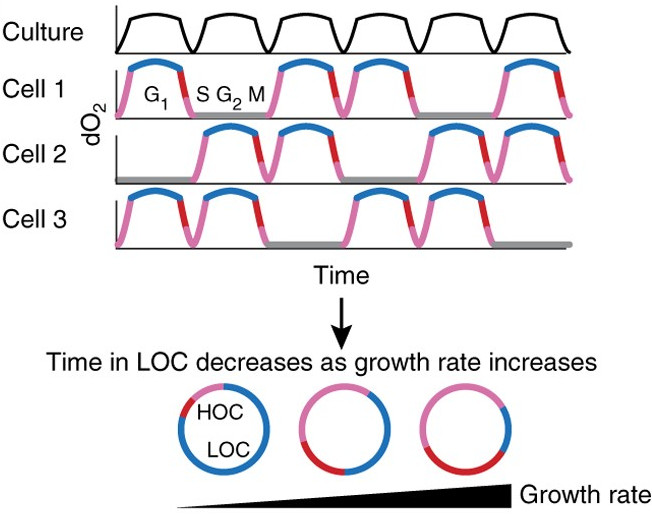
\includegraphics[width=0.8\textwidth]{mellorMolecularBasisMetabolic2016_3b_adapted}
  \caption[
    Model for how sub-populations of cells may account for oscillations of dissolved oxygen observed in the chemostat
  ]{
    Model for how sub-populations of cells may account for oscillations of dissolved oxygen observed in the chemostat.
    Cells may enter the cell division cycle (pink-blue-red lines), gated by the metabolic cycle, in a staggered manner, and the combined effect of all cells may explain dissolved oxygen concentrations (black lines, top row).
    Adapted from \textcite{mellorMolecularBasisMetabolic2016}.}
  \label{fig:intro-ymc-populations}
\end{figure}

The chemostat obscures contribution of sub-populations of cells (Fig.\ \ref{fig:intro-ymc-populations}).
\textcite{burnettiCellCycleStart2016} suggest that sub-populations within the yeast culture that enter the yeast metabolic cycle in a staggered manner can be responsible for chemostat observations, as evidenced by how the yeast cells spend proportionately more time in the reductive phase at lower dilution rates.
Contributions from sub-populations of cells are further highlighted by \textcite{bagameryPutativeBetHedgingStrategy2020}, who used a microfluidic platform to show that a group of genetically identical yeast cells divide themselves into two populations.
Such a bet-hedging strategy results in some percentage of the population surviving in a glucose-starved or a glucose-rich condition, beneficial for long-term population survival.
Taken together, it is possible that phenotypically different sub-populations in the chemostat culture may partially explain the observations in the chemostat so far.
In addition, there is the question of whether cells individually generate the metabolic cycle or is a diffusible chemical responsible for synchrony, as proposed by \textcite{krishnaMinimalPushPull2018}.
Furthermore, \textcite{smithTheoryChemostatDynamics1995} shows, theoretically, that a chemostat with two competing species with an inhibitor added to the chemostat that inhibits one of the competitors can generate oscillations.
In the case of the yeast metabolic cycle, the competitors can be genetically identical sub-populations of the yeast cells that have different levels of sensitivities to an inhibitor, perhaps a metabolic by-product.
Bulk culture set-ups, including chemostats, are not able to address questions about cell sub-populations and autonomy of the metabolic cycle.
However, single-cell set-ups may fill in such a technical gap.

Finally, the chemostat imposes glucose starvation, and single-cell studies with different carbon sources give a different picture in terms of metabolic requirements.
Chemostat studies and related models suggest that glucose starvation and oxidative metabolism are required for oscillations in dissolved oxygen level that define YMCs.
NAD(P)H oscillations have been recorded in non-fermentative conditions, such as pyruvate or low-glucose media \parencite{papagiannakisAutonomousMetabolicOscillations2017}.
However, NAD(P)H \parencite{papagiannakisAutonomousMetabolicOscillations2017,ozsezenInferenceHighLevelInteraction2019} and flavin \parencite{baumgartnerFlavinbasedMetabolicCycles2018} oscillations still occur in constant high-glucose conditions, and only within a window of periods, in contrast to the 1.4--14 hour range reported for chemostat-based studies.
Furthermore, \textit{ATP5} and \textit{CYT1} deletions that impair oxidative respiration do not remove single-cell flavin-based metabolic oscillations \parencite{baumgartnerFlavinbasedMetabolicCycles2018}, thus giving additional evidence that oxidative metabolism is not required for the YMC.

Single-cell microfluidic studies are well-positioned to address the limitations of the chemostat,
although there have been only few studies.
\textcite{laxmanBehaviorMetabolicCycling2010} was an early attempt at using microfluidics to address the bulk vs single-cell issue by culturing strains with fluorescent gene expression reporters for each phase (OX, RB, RC) of the metabolic cycle by transferring cycling cells from a chemostat to a microfluidic device for real-time imaging of the cells.
The study showed that low glucose levels were required for the synchrony of metabolic cycles across cells.
This study also shows the presence of quiescent cells, and then proposed that during OX phase, cells decide whether to commit to cell growth or enter a quiescent state, leading to a model of two subpopulations in the culture.
However, it lacks quantitative time-series analysis, rather, reporting qualitative interpretations of fluorescence images.
The microfluidic device did not truly physically separate each cell individually, thus it was unable to eliminate the possibility of cell-to-cell communication via a diffusible signalling chemical.
% This does seen like a key difference seen in single-cell, but the fact wasn't made clear
% in writing here.
\textcite{papagiannakisAutonomousMetabolicOscillations2017} revealed that YMCs are an intrinsic feature of single cells and are autonomous with respect to the cell division cycle, based on measurements of the combined level of NADH and NADPH in single cells in microfluidic devices.
Furthermore, by measuring flavin fluorescence in the cell, \textcite{baumgartnerFlavinbasedMetabolicCycles2018} demonstrated that YMCs persist in mutants deficient in oxidative phosphorylation, and that the cell division cycle inhibitor rapamycin desynchronises the YMC and the cell division cycle.
In sum, these single-cell studies address a small fraction of the knowledge covered by chemostat studies, and further such studies are required.


\subsubsection{Molecular and genetic mechanisms}
\label{subsubsec:intro-ymc-unresolved-molecular}

There are unknowns in the molecular mechanism that drives YMCs.
Genome-wide transcript cycling has two superclusters that correspond to the oxidative and reductive-building phases \parencite{machneYinYangYeast2012}.
However, there has been no genome-wide analysis of genes that influence cycling \parencite{mellorMolecularBasisMetabolic2016}, though some genes seem to have key roles.
As we lack proteome analysis, it is unclear how protein levels and post-translation modifications are affected.

%[FIGURE: MY INVESTIGATION OF CAMPBELL ET AL. 2020 TO SHOW PERIODICITY OF TRANSCRIPTS/PROTEINS/METABOLITES]

Metabolome cycling may play a role in the metabolic cycle and can explain temporal partitioning of biosynthesis, but the evidence so far is indirect as it is based on the cell division cycle.
\textcite{campbellBuildingBlocksAre2020} showed that lipid biosynthesis in budding yeast is periodic with the cell division cycle and peaks during S phase, as evidenced by an increase in the number of metabolites implicated in lipid metabolism in such phases, based on metabolomics analysis of prototrophic cells with synchronised cell division cycles.
Here, precursors are synthesised as they are needed.
\textcite{ewaldYeastCyclinDependentKinase2016} also show that the cell division cycle machinery regulate trehalose mobilisation, showing the coupling between carbohydrate store levels and cellular oscillators.
They also showed that lipid metabolism increased during S/G2/M, likely due to the synthesis of new cell membranes during bud growth, as evidenced by pathway enrichment analysis.
Based on the coupling between the yeast metabolic cycle and the cell division cycle, it can be inferred that lipid store cycling and perhaps to a lesser extent carbohydrate store cycling are likely instrumental to the yeast metabolic cycle.
Though, investigation of how an impairment in lipid utilisation affects the yeast metabolic cycle in single cells is needed to truly prove that such cycles are responsible for the metabolic cycle.
% [REMOVE THIS SENTENCE, OR REWORD AS DISCUSSION OF EVIDENCE]
% Preferably, I need evidence to support metabolome cycles that also confirms that the YMC is independent of the cell division cycle.

%Additionally, the effects of perturbations to specific metabolic networks in single-cell conditions are yet to be determined [EVIDENCE NEEDED].

\subsection{Implications of the metabolic cycle}
\label{subsec:intro-ymc-implications}

%- campbell et al. 2020: suggests temporal regulation of biosynthesis for cell division cycle -- similar logic to ymc?  can put this in implications of ymc section

The YMC shares regulatory mechanisms with the cell division cycle and the circadian rhythm,
leading to the question of whether the metabolic cycle reflects a fundamental system.

% Describe metabolic cycles in other organisms...
Similar metabolic cycles have been described in other organisms.
\textit{E. coli} shows oscillations in NAD(P)H fluorescence coupled to its cell division cycle, as evidenced by time-lapse microscopy of single cells \parencite{zhangDynamicSinglecellNAD2018}.
Addition of glucose or hydrogen peroxide to the medium results in global changes in autofluorescence, reflecting a response to nutrient conditions.
Metabolic cycles have been observed in mammalian cells.
For example, \textcite{zhuLogicTemporalCompartmentalization2022} describe a 12-hour metabolic cycle in liver cells that includes temporal partitioning of metabolic processes into energy homeostasis, genetic integrity maintenance processes, immune response, and gene expression --- linking the processes to the circadian rhythm and the whole cycle to a more general 12-hour mammalian ultradian clock.
Importantly, this hepatic metabolic cycle operates independently from the spatial organisation of cells in the liver, reminiscent of the autonomy of the yeast metabolic cycle.
In addition, HeLa cells with synchronised cell division have been shown to exhibit both NAD(P)H and ATP oscillations throughout the cell division cycle \parencite{ahnTemporalFluxomicsReveals2017}, but the literature is conflicted about the these oscillations' dynamics across different mammalian cell types \parencite{zylstraMetabolicDynamicsCell2022}.
There is reason to believe that a wide range of organisms exhibit biochemical phenomena similar to the yeast metabolic cycle, as the aims of controlling cell division to match environmental conditions along with the temporal coordination of biosynthesis and cellular redox state with cell division should be fundamental goals that apply to multiple domains of life.

%- Fundamental mechanistic basis for biological oscillators, such as the cell division cycle.  Could change what we know about the cell division cycle.
% (Significance of study)
Metabolic oscillations may be the origins of biological timekeeping mechanisms.
\textcite{lloydRedoxRhythmicityClocks2007} assert that ultradian oscillations form the basis of longer-period biological oscillators like the circadian rhythm or the cell cycle, based on temperature compensation and sensitivity of the period.
It is logical for a biological oscillation to have temperature compensation because temperature oscillates with a period of a day on most of the planet.
Circadian rhythms can occur in cells of multicellular eukaryotes without transcription \parencite{oneillCircadianRhythmsPersist2011}, refuting the idea that gene circuits are responsible for such rhythms.
Additionally, the eukaryotic cell cycle evolved before cyclin-dependent kinases \parencite{papagiannakisAutonomousMetabolicOscillations2017}, so metabolic oscillations may have served to regulate the cell cycle before cyclin-dependent kinases evolved.
Furthermore, YMCs share mechanisms with the circadian oscillator \parencite{caustonMetabolicCyclesYeast2015,arataQuantitativeStudiesCellDivision2019}, suggesting a common evolutionary origin.
Thus, studying YMCs may shed light on the evolution of biological rhythms.

A philosophical question that unites all biological oscillators is: why have oscillations?
The answers may differ for each type of biological oscillator.

The answer is clear for circadian rhythms: circadian clocks evolved as an adaptation to the Earth's 24-hour rotation, and allow organisms to match biological processes that benefit from light or warmth to the time of day at which they occur \parencite{millarInputSignalsPlant2004}.
The selective advantage of such a system is highlighted by how circadian clocks of similar, negative-feedback gene circuit architectures evolved independently at least four times across kingdoms \parencite{doddPlantCircadianClocks2005}.
As a specific example, \textit{Arabidopsis thaliana} plants with a clock period matched to the environment contain more chlorophyll, fix more carbon, grow faster, and survive better, as opposed to mutants with clock lengths that do not match environmental light-dark cycles \parencite{doddPlantCircadianClocks2005}.
The explanation is: light-harvesting complex proteins and chlorophyll are unstable in their unbound state.
So, synthesising these components in sync with the light-dark cycle is advantageous for the plant.
The plant can only do so with correct anticipation of dawn and dusk, and a circadian clock that matches the environmental light-dark cycle allows this to happen.

The importance of coordinating the sequence of events in the cell division cycle was discussed in section~\ref{subsec:intro-ymc-biological_rhythms}.
Briefly, the cell division cycle is an energy-intensive and resource-intensive process that engages all compartments of the cell.
In addition, maintaining genetic fidelity is important for ensuring that progeny cells are functional, therefore, cells need a robust system of tight control of the cell division cycle.
The importance of the cell division cycle is highlighted by the conserved design of the cell division cycle across kingdoms.
For example, cyclin-dependent kinases (CDKs) differ in their number in different organisms --- one in budding yeast, but at least 11 classical CDKs in humans \parencite{malumbresCyclindependentKinasesFamily2009} --- but their structure and function are conserved.
The importance of linking the cell division cycle with cellular resource use is highlighted by the cell's systems of coupling the cell division cycle machinery with metabolic processes \parencite{salazar-roaFuelingCellDivision2017}.
In particular, oxidative phosphorylation peaks upon S- and M-phase entry in plants and glycolysis peaks upon S-phase entry in lymphocytes.
In addition, the CDKs regulate cycles of mitochondrial fusion and fission to ensure that mitochondria in the parent cell are divided to progeny cells based on their volumes.
The importance of the cell division cycle control system is further highlighted by the result of impairments in the genetic control of the cell division cycle: uncontrolled cell proliferation, characteristic of cancers in multicellular organisms.

The question of `why have oscillations?' has been asked of the yeast metabolic cycle --- specifically, why cycle metabolites and why cycle transcripts?
It has been proposed that cycling of metabolites and metabolic activity serve to create `just-in-time' biosynthesis of compounds when they are needed in the yeast metabolic cycle \parencite{zylstraMetabolicDynamicsCell2022}.
For example, the HOC phase of the metabolic cycle is driven by the high energetic demands of protein synthesis in this phase, which is closely linked to the G\textsubscript{1} phase of the cell division cycle \parencite{oneillEukaryoticCellBiology2020}, and the evidence includes high protein synthesis rate and high ribosomal protein abundance.
The rationale for cycling transcripts is less clear, however.
Earlier studies propose that transcript cycling in clusters that peak according to three metabolic cycle phases reflect the metabolic demands in each phase and the translation of such transcripts lead to changes in metabolite concentrations \parencite{tuLogicYeastMetabolic2005}.
However, \textcite{felthamTranscriptionalChangesAre2020} showed that although transcripts levels cycle, protein levels chiefly remain constant, but post-translational modifications cycle instead.
This study then proposes that cyclic metabolic state changes cause post-translational modifications which then coordinate the metabolic cycle with cellular processes.
The study therefore suggests that transcript cycling is effect of the metabolic cycle and have roles in the chromatin environment.
Further clarification of the mechanistic basis of the yeast metabolic cycle is needed to answer the `why have oscillations' question.

\section{Flavins and flavoproteins}
\label{sec:intro-flavin}

\subsection{Introduction to cellular autofluorescence}
\label{subsec:intro-flavin-autofluo}
% - (Refer to reviews, e.g. Maslanka et al. 2018 -- is a goldmine)

Cellular autofluorescence is defined as the intrinsic fluorescence of a cell without fluorescent tags.
It is caused by the autofluorescence of compounds that have light emission properties \parencite{maslankaAutofluorescenceYeastSaccharomyces2018}.
Such endogenous fluorophores include coenzymes, vitamins, and amino acids with aromatic chemical groups, flavins being one of them.
However, autofluorescence pose difficulty in cellular microscopy because their wavelengths can overlap with other fluorophores and therefore it is difficult to draw biochemical conclusions from the signal alone.
For example, flavin autofluorescence overlaps with the spectrum of the fluorescent glucose analogue 6-NBDG \parencite{maslankaAutofluorescenceYeastSaccharomyces2018}, and thus interferes with studies that use this analogue to study glucose uptake.
Owing to the identity of the compounds that are responsible for autofluorescence, cellular autofluorescence can indicate of the physiology and metabolism of the cell, and it has been used to study the yeast metabolic cycle.
Autofluorescence thus offers an easy way to monitor cell physiology without engineering genetic constructs.

\subsection{Biochemical basis of flavins and flavoproteins}
\label{subsec:intro-flavin-biochem}

\begin{figure}
  \centering
  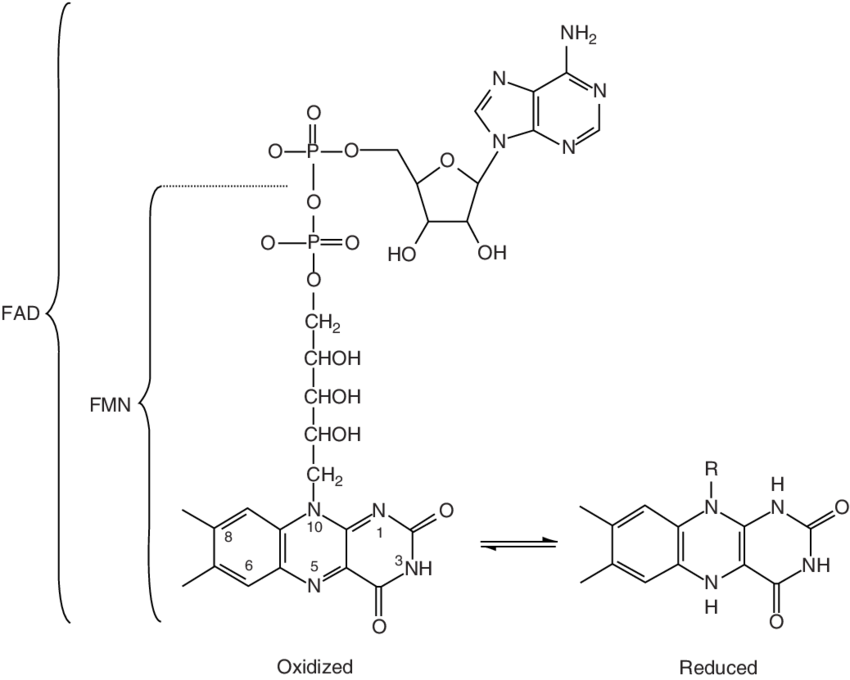
\includegraphics[width=0.7\textwidth]{patelFlavinContainingOxidativeBiocatalysts2006_1}
  \caption[
    Chemical structure of FMN and FAD
  ]{
    Chemical structure of FMN and FAD, with redox states of the aromatic flavin moiety shown.
    Adapted from \textcite{patelFlavinContainingOxidativeBiocatalysts2006}.}
  \label{fig:intro-flavin-structure}
\end{figure}

Flavins are a group of organic compounds that share an aromatic moiety that allows redox reactions (Fig.\ \ref{fig:intro-flavin-structure}).
Specifically, the flavin moiety can exist in the oxidised, semiquinone, or reduced states.
Flavins thus function as electron carriers in the cell.
In \textit{Saccharomyces cerevisiae}, flavin is present as FMN and FAD, which function as prosthetic groups in flavin-dependent proteins, or flavoproteins, whose genes account for 1.1\% of the genome \parencite{gudipatiFlavoproteomeYeastSaccharomyces2014}.
FMN and FAD can be covalently bound to these proteins or be free \parencite{mewiesCovalentAttachmentFlavin1998}.
FAD is a co-enzyme and has major roles in transferring electrons from the TCA cycle to the mitochondrial ETC.
Flavins in \textit{Saccharomyces cerevisiae} are derived from riboflavin (Fig.\ \ref{fig:intro-flavin-schematic}).
Riboflavin can be synthesised \textit{de novo} from purine biosynthesis and the oxidative pentose phosphate pathway (Fig.\ \ref{fig:intro-flavin-kegg}).
% Is there more to this than the KEGG diagram?
Based on the metabolism of flavins, the cell only synthesises new flavin for synthesis of FMN and FAD.

% (Biosynthesis of flavin)

\begin{figure}
  \centering
  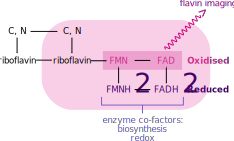
\includegraphics[width=0.9\textwidth]{flavin-cell-schematic}
  \caption[
    Simplified schematic of biosynthesis of flavins
  ]{
    Simplified schematic of biosynthesis of flavins and detection of the oxidation states in fluorescence microscopy.
    }
  \label{fig:intro-flavin-schematic}
\end{figure}

% https://www.genome.jp/pathway/map00740
\begin{figure}
  \centering
  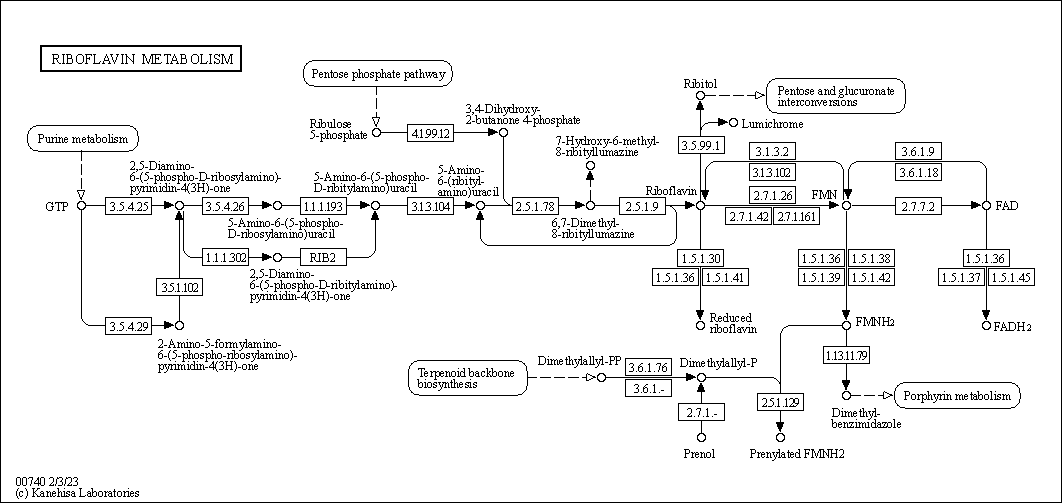
\includegraphics[width=0.95\textwidth]{kegg-flavin}
  \caption[
    Reference pathway for biosynthesis of riboflavin and derivatives
  ]{
    Reference pathway for biosynthesis of riboflavin and derivatives, KEGG pathway database \parencite{kanehisaKEGGTaxonomybasedAnalysis2023}.
    }
  \label{fig:intro-flavin-kegg}
\end{figure}

\begin{figure}
  \centering
  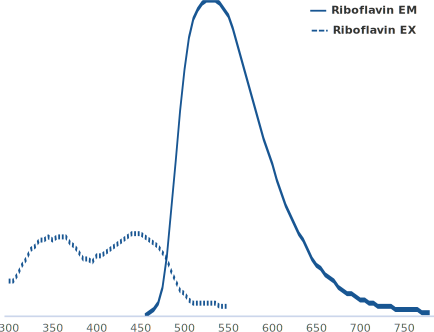
\includegraphics[width=0.95\textwidth]{fpbase-riboflavin-adapted}
  \caption[
    Fluorescence spectrum of riboflavin
  ]{
    Fluorescence spectrum of riboflavin, (dotted line) excitation and (solid line) emission spectra shown, FPbase \parencite{lambertUsingFPbaseFluorescent2023}.
    }
  \label{fig:intro-flavin-spectra}
\end{figure}

From a technical standpoint, the redox states of flavins reflect the emission and absorption of electromagnetic radiation by the flavin moiety.
The redox biochemistry of flavins give rise to fluorescence, so monitoring flavin autofluorescence monitors the redox state of the cell.
Flavins, in their oxidised forms (FMN and FAD), have a peak excitation frequency of $\approx$460 nm and a peak emission frequency of $\approx$535 nm \parencite{maslankaAutofluorescenceYeastSaccharomyces2018, wagnieresVivoFluorescenceSpectroscopy1998}, displayed in Fig.\ \ref{fig:intro-flavin-spectra}.
Comparison of \textit{in vivo} autofluorescence in mammalian cells and the fluorescence spectrum of riboflavin in PBS confirms this fluorescence behaviour \parencite{aubinAutofluorescenceViableCultured1979}.
In contrast, the reduced forms FMNH\textsubscript{2} and FADH\textsubscript{2} have negligible fluorescence \parencite{mastersConfocalRedoxImaging1994}.
Both chemostat-based \parencite{sasidharanTimeStructureYeastMetabolism2012, murrayRedoxRegulationRespiring2011} and single-cell microfluidic studies \parencite{baumgartnerFlavinbasedMetabolicCycles2018} have monitored flavin autofluorescence to study the YMC.

\subsubsection{Descriptions of key flavoproteins and their roles}
\label{subsubsec:intro-flavin-biochem-descriptions}
% - (Sort by abundance)
% - (On second thought, I'm not sure how useful a shopping list of flavoproteins is.
% probably better to pick a couple that are really key to what i study)

\begin{figure}
  \centering
  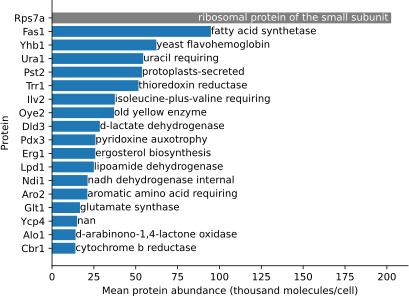
\includegraphics[width=0.9\textwidth]{flavoprotein_abundance_bar}
  \caption[
    Flavoproteins shown by abundance
  ]{
    Flavoproteins (blue bars) shown by abundance \parencite{hoUnificationProteinAbundance2018}, with Rps7ap (grey bar) shown as reference.
    Only the 17 most abundant flavoproteins are shown.
    }
  \label{fig:intro-flavoprotein-abundance}
\end{figure}

\textcite{gudipatiFlavoproteomeYeastSaccharomyces2014} describe 68 genes that code for 47 flavoproteins in budding yeast (Fig.\ \ref{fig:intro-flavoprotein-abundance}).
Of these, 35 require FAD, 15 require FMN, and 3 require both.
In budding yeast, most flavins sit in the active site without covalent bonding.
The biochemical and enzymatic properties of many flavoproteins are poorly characterised \parencite{kochStructureBiochemicalKinetic2017}.

\begin{table}[htbp]
  \footnotesize
  \centering
  % Control spacing between rows
  \renewcommand{\arraystretch}{2}
  \begin{tabularx}{\linewidth}{sbbs}
    \toprule
    Protein & Name & Reaction catalysed & Reference\\
    \midrule
    Fas1 & beta subunit of fatty acid synthetase & \ce{acetyl-CoA + malonyl-CoA + NADPH + ATP -> palmitate} & \textcite{singhDiscoveryRegulatorySubunit2020} \\
    Yhb1 & nitric oxide oxidoreductase & \ce{2NO + 2O2 + NAD(P)H -> 2NO3- + NAD(P)+ + H+} & \textcite{bonamoreFlavohemoglobinStructureReactivity2008} \\
    Ura1 & dihydroorotate dehydrogenase & \ce{dihydroorotic acid + fumarate -> orotic acid + succinate} & \textcite{zameitatDihydroorotateDehydrogenaseSaccharomyces2007} \\
    Pst2 & NAD(P)H-quinone oxidoreductase & \ce{NAD(P)H + H+ + quinone -> NAD(P)+ + hydroquinone} & \textcite{kochStructureBiochemicalKinetic2017} \\
    Trr1 & cytoplasmic thioredoxin reductase & \ce{H+ + NADPH + thioredoxin disulfide -> NADP+ + thioredoxin} & \textcite{machadoThioredoxinReductasedependentInhibition1997} \\
    Ilv2 & acetolactate synthase & \ce{2 pyruvate -> 2-acetolactate + CO2} & \textcite{pangCrystalStructureYeast2002} \\
    Oye2 & NADPH oxidoreductase & \ce{NADPH + H+ + acceptor <--> NADP+ + reduced acceptor} & \textcite{odatOldYellowEnzymes2007} \\
    Dld3 & 2-hydroxyglutarate transhydrogenase & \ce{D-2-hydroxyglutarate + pyruvate -> \alpha-ketoglutarate + lactate} & \textcite{becker-ketternSaccharomycesCerevisiaeForms2016} \\
    Pdx3 & pyridoxine phosphate oxidase & \ce{pyridoxamine 5-phosphate + H2O + O2 -> pyridoxal 5-phosphate + NH3 + H2O} & \textcite{tsugePurificationPropertiesPyridoxamine1979} \\
    Erg1 & squalene epoxidase & \ce{squalene + H+ + NADPH + O2 -> 2,3-oxidosqualene + NADP+ + H2O} & \textcite{satohEnzymaticPropertiesSqualene1993} \\
    Lpd1 & dihydrolipoamide dehydrogenase & \ce{dihydrolipoamide + NAD+ -> lipoamide + NADH+ + H+} & \textcite{morrisonChapter14Dihydrolipoamide2021} \\
    \bottomrule \\
  \end{tabularx}
  \caption{
    Roles of the most abundant flavoproteins.
  }
  \label{tab:intro-flavoproteins}
\end{table}

The most abundant flavoproteins catalyse redox reactions (table~\ref{tab:intro-flavoproteins}).
Specifically, these reactions include reduction of reactive chemical species to respond to oxidative stress --- though not all enzymes involved in the response to reactive chemical species have flavin co-factors.
Additionally, the reactions include biosynthetic reactions.
Many of these reactions require NADPH or NADH to donate electrons, suggesting a link between flavins and NAD(P)H in regulating the cellular redox state.
In particular, Oye2p catalyses the NADPH redox reaction, thus providing a link between flavins and NAD(P)H.
One exception flavoprotein is Ilv2p, which does not catalyse a redox reaction.
It has been hypothesised that an ancestral form of Ilv2p catalysed a redox reaction, but the argument is weak because it is inferred from the presence of FAD \parencite{pangCrystalStructureYeast2002}.
To maintain the cellular redox state, it is thus reasonable to assume that the redox equilibrium of all flavoprotein-catalysed reactions are in the same direction at any point of the YMC.
Supporting this, \textcite{sianoNADHFlavinFluorescence1989} show that NAD(P)H fluorescence and the fluorescence of lipoamide dehydrogenase, a flavoprotein, indicate simultaneous reduction in response to lowered dissolved oxygen.
They further show redox equilibrium in both fluorophores in response to glucose addition.

It is important to rule out the possibility that flavin cycling is merely a function of the cell division cycle to make sure that flavin monitoring monitors the YMC.
None of these flavoproteins are strictly cell division cycle proteins, but this does not exclude cycling of flavin autofluorescence linked to the cell division cycle.
For example, fatty acid synthesis proteins should cycle along with the cell division cycle as cell synthesises more plasma membrane.

\subsection{Flavins and flavoproteins in the yeast metabolic cycle}
\label{subsec:intro-flavin-ymc}

Flavin fluorescence can be used to monitor the metabolic cycle.
The biological basis of flavins justifies this use.
Flavins are linked to NAD(P)H via nitric oxide oxidoreductase (Yhb1p), as discussed in section \ref{subsubsec:intro-flavin-biochem-descriptions}, and NAD(P)H cycles have been implicated in bulk-culture \parencite{tuLogicYeastMetabolic2005} % and more
and single-cell \parencite{papagiannakisAutonomousMetabolicOscillations2017} studies of the YMC, as discussed in section \ref{subsubsec:intro-ymc-definition-phases}.
The oxidation of flavin is at its maximum at the start of the reductive state of the YMC, as evidence by how flavin fluorescence peaks just before dissolved oxygen concentration in the chemostat \parencite{murrayRedoxRegulationRespiring2011,sasidharanTimeStructureYeastMetabolism2012}.
Riboflavin abundance in the cell has been shown to oscillate and peak in the oxidative state of the YMC, while FAD abundance is at its maximum in the reductive-building phase, as evidenced by metabolic profiling of extracts from chemostat cultures taken at evenly-spaced intervals \parencite{tuCyclicChangesMetabolic2007}.
Flavoproteins may have roles linked to the YMC.
The most abundant is Fas1 (fatty acid synthetase).
Because there is evidence that cycles of fatty acid stores are implicated in metabolic cycling in yeast \parencite{campbellBuildingBlocksAre2020}, it is likely that fatty acid synthetase is heavily implicated.
Following this, the second most abundant is Yhb1, which may play a major role as discussed earlier.

So, for these reasons, I expect flavin autofluorescence to be oscillatory and be a useful readout of the yeast metabolic cycle.
Few studies have characterised how such flavin oscillations respond to changing nutrient conditions or to gene deletions.
Thus, filling in this knowledge gap is an avenue for further research.

Nevertheless, there are caveats to using flavin autofluorescence.
Riboflavin fluorescence is captured too, though its intracellular abundance is two order of magnitudes lower than that of FMN and that of FAD, and these two flavin derivatives are present at the same order of magnitude \parencite{tuCyclicChangesMetabolic2007}.
Plus, different concentrations of riboflavin influence the autofluorescence signal and influence the physiological state of the cell \parencite{maslankaAutofluorescenceYeastSaccharomyces2018}.
The experimenter can eliminate the effects of riboflavin by using riboflavin-free minimal media \parencite{verduynEffectBenzoicAcid1992}.
Additionally, flavin fluorescence is the aggregate of many flavoprotein components, therefore it cannot be concluded that flavin fluorescence is the readout of one protein in particular --- one can only draw conclusions about the overall redox state.
Furthermore, the changes in flavin fluorescence can be because of changes in the `flavin pool' --- the amount of flavin-derived moieties in a cell across all their redox states --- or due to global changes in intracellular flavin redox state, as a function of intracellular redox state.
Most studies assume a constant flavin pool and see oscillations as periodic shifts in redox equilibrium.
These caveats are not unique to flavin fluorescence, but are shared limitations with other auto-fluorescing cellular components like NAD(P)H, and the benefits of having a non-invasive method to monitor cellular metabolism outweighs the caveats.

%%% Local Variables:
%%% mode: latex
%%% TeX-master: "../thesis.tex"
%%% End:

% % ROUGH DRAFT, based on 10-month report for now
% PROBABLY BEST WRITTEN AFTER BIOLOGICAL RESULTS CHAPTER DRAFT DONE
% TODO:

\chapter{Methods}
\label{ch:methods}

\section{Strains and media}
\label{sec:methods-strains_media}

The \emph{S. cerevisiae} strains used in this thesis are described in table~\ref{tab:methods-strains}.
% Potential additions: CEN.PK & Causton strains, if they go into the biological chapter.

\begin{table}
  \footnotesize
  \centering
  \begin{tabularx}{\linewidth}{bbbbb}
    \toprule
    Name & Background & Genotype & Origin & Notes\\
    \midrule
    FY4 & FY4 & - & EUROSCARF & \textcite{winstonConstructionSetConvenient1995} \\
    htb2::mCherry & FY4 & HTB2::mCherry & In-house, CRISPR & - \\
    BY4741 & BY4741 & \emph{MAT}a \emph{his3$\Delta$1 leu2$\Delta$0 met15$\Delta$0 ura3$\Delta$0} & EUROSCARF & \textcite{brachmannDesignerDeletionStrains1998}\\
    zwf1$\Delta$ & BY4741 & zwf1$\Delta$::KAN & Edinburgh Genome Foundry & Yeast deletion collection \\
    BY4742 & BY4742 & \emph{MAT}a \emph{his3$\Delta$1 leu2$\Delta$0 lys2$\Delta$0 ura3$\Delta$0} & Bruce Morgan & \textcite{calabreseHyperoxidationMitochondrialPeroxiredoxin2019}\\
    tsa1$\Delta$ tsa2$\Delta$ & BY4742 & tsa1$\Delta$::natNT2 tsa2$\Delta$::kanMX4 & Bruce Morgan & \textcite{calabreseHyperoxidationMitochondrialPeroxiredoxin2019} \\
    \bottomrule \\
  \end{tabularx}
  \caption{Strains used in this thesis.}
  \label{tab:methods-strains}
\end{table}

The minimal medium described by \parencite{verduynEffectBenzoicAcid1992} was used unless otherwise stated.
This minimal medium does not contain riboflavin, thus minimising its effect on flavin autofluorescence imaging, and its composition is known and easily-controlled.
Specifically, the composition of the carbon source-limiting medium are described in tables~\ref{tab:methods-media-delft}--\ref{tab:methods-media-delft-vitamins}, and the media pH was adjusted to 6.0 before use using potassium hydroxide, or sodium hydroxide for potassium-free media.
For auxotrophic strains, supplements were added according to table~\ref{tab:methods-media-auxotroph}.
Then, a carbon source is added as appropriate to create the growth medium.

% TODO: align numbers by their decimal point
\begin{table}
  \footnotesize
  \centering
  \begin{tabularx}{\linewidth}{bbb}
    \toprule
    Reagent & Concentration & Remarks\\
    \midrule
    \ce{KH2PO4} & \SI{3.}{\gram~\litre^{-1}} & \\
    \ce{MgSO4.7H2O} & \SI{0.5}{\gram~\litre^{-1}} & \\
    \ce{(NH4)2SO4} & \SI{5.}{\gram~\litre^{-1}} & \\
    \ce{Trace metals} & \SI{1.}{\milli\litre~\litre^{-1}} & See table~\ref{tab:methods-media-delft-metals} \\
    \ce{Vitamins} & \SI{1.}{\milli\litre~\litre^{-1}} & See table~\ref{tab:methods-media-delft-vitamins}.  Add upon use. \\
    \ce{Carbon source} & variable & Add upon use. \\
    \bottomrule \\
  \end{tabularx}
  \caption{
    Composition of base minimal medium.
    For potassium-free media, replace \ce{KH2PO4} with \SI{2.65}{\gram~\litre^{-1}} \ce{NaH2PO4}, which gives the same molarity.
  }
  \label{tab:methods-media-delft}
\end{table}

\begin{table}
  \footnotesize
  \centering
  \begin{tabularx}{\linewidth}{bbb}
    \toprule
    Reagent & Formula & Concentration [\SI{}{\gram~\litre^{-1}}]\\
    \midrule
    EDTA & \ce{C10H14N2Na2O8.2H2O} & 15.00 \\
    Zinc sulfate & \ce{ZnSO4.7H2O} & 4.50 \\
    Manganese (II) chloride & \ce{MnCl2.2H2O} & 0.84 \\
    Cobalt (II) chloride & \ce{CoCl2.6H2O} & 0.30 \\
    Copper (II) sulfate & \ce{CuSO4.5H2O} & 0.30 \\
    Sodium molybdate & \ce{Na2MoO4.2H2O} & 0.40 \\
    Calcium chloride & \ce{CaCl2.2H2O} & 4.50 \\
    Iron (II) sulfate & \ce{FeSO4.7H2O} & 3.00 \\
    Boric acid & \ce{H3BO3} & 1.00 \\
    Potassium iodide & \ce{KI} & 0.10 \\
    \bottomrule \\
  \end{tabularx}
  \caption{
    Composition of trace metal mix for minimal media described in table~\ref{tab:methods-media-delft}.
  }
  \label{tab:methods-media-delft-metals}
\end{table}

\begin{table}
  \footnotesize
  \centering
  \begin{tabularx}{\linewidth}{bbb}
    \toprule
    Reagent & Formula & Concentration [\SI{}{\gram~\litre^{-1}}]\\
    \midrule
    D-(+)-biotin & \ce{C10H16N2O3S} & 0.05 \\
    D-panthothenic acid calcium salt & \ce{Ca(C9H16NO5)2} & 1.00 \\
    Nicotinic acid & \ce{C6H5NO2} & 1.00 \\
    \emph{myo}-Inositol & \ce{C6H12O6} & 25.00 \\
    Thiamine chloride hydrochloride & \ce{C12H15ClN4OS.HCl} & 1.00 \\
    Pyridoxal hydrochloride & \ce{C8H12ClNO3} & 1.00 \\
    4-aminobenzoic acid & \ce{C7H7NO2} & 0.20 \\
    \bottomrule \\
  \end{tabularx}
  \caption{
    Composition of vitamin mix for minimal media described in table~\ref{tab:methods-media-delft}.
  }
  \label{tab:methods-media-delft-vitamins}
\end{table}

\begin{table}
  \footnotesize
  \centering
  \begin{tabularx}{\linewidth}{bbb}
    \toprule
    Reagent & Concentration [\SI{}{\milli\gram~\litre^{-1}}] \\
    \midrule
    histidine & 125. \\
    leucine & 500. \\
    tryptophan & 75. \\
    methionine & 100. \\
    uracil & 150. \\
    \bottomrule \\
  \end{tabularx}
  \caption{
    Supplements to minimal media for BY4741-background auxotrophic strains, compositions derived from \textcite{pronkAuxotrophicYeastStrains2002}.
    For BY4742-background strains, replace methionine with \SI{100}{\milli\gram~\litre^{-1}} lysine-HCl.
  }
  \label{tab:methods-media-auxotroph}
\end{table}

\section{Single-cell microfluidics}
\label{sec:methods-microfluidics}

Cells were grown in a minimal media formulation appropriate for the experiment, supplements appropriate for the strain's auxotrophy, and a carbon source (glucose or pyruvate) appropriate for the experiment (see section~\ref{sec:methods-strains_media}).
% Kevin's OD measurements?
After \SI{14}{hr} overnight growth, the cells were diluted so that the resulting culture had an OD\textsubscript{600} of 0.10--0.20, and then were incubated for \SI{4}{hr} at \SI{30}{\celsius}.

% Refer to Jove paper if it comes out
ALCATRAS microfluidics \parencite{craneMicrofluidicSystemStudying2014}  chambers were filled with media supplemented with 2\% w/v glucose and 0.05\% w/v bovine serum albumin.
Cells were then loaded into the ALCATRAS chambers.
Syringe pumps containing media were programmed to produce a constant flow of \SI{4}{\micro\litre} into the chambers.
The cells and ALCATRAS chambers were located in an incubation chamber (Oko-labs) that was maintained at \SI{30}{\celsius}.

% Update fluorescence settings
Microscopy was performed using a 60 $\times$ 1.4 NA oil immersion objective (Nikon), and the Nikon Perfect Focus System was used to ensure consistent focus.
Five z-slices were taken for brightfield images, with a spacing of \SI{0.6}{\nano\metre} between slices.
Fluorescence imaging was performed with an OptoLED light source (Cain Research), and LED voltage was optimised for maximum signal intensity without LED cut-off prior to experiments.
For flavin imaging, the excitation frequency was \SI{430}{\nano\metre}, the emission filter was set to \SI{455}{\nano\metre}, and exposure time varied: \SI{0}{\milli\second}, \SI{60}{\milli\second}, \SI{120}{\milli\second}, and \SI{180}{\milli\second}.
For mCherry imaging, the excitation frequency was \SI{590}{\nano\metre} and the exposure time was \SI{100}{\milli\second}.
Z-slices were taken for the mCherry images, with the same number of slices and spacing as for the brightfield images.
Image acquisition duration varied for each experiment.
For all channels, images were taken every \SI{5}{min}.

\section{Segmentation, extraction, post-processing}
\label{sec:methods-segmentation}

% TODO: Most of this is obsolete.  Update for aliby.

The brightfield z-stack images were segmented using custom neural network-based software based in MATLAB.
The software identified cell boundaries, birth events, and cell lineages.

Because the aperture of the microscope causes optical aberration, aperture-fitting and flat-field corrections were performed for the flavin and mCherry channels independently, using custom MATLAB scripts.
First, the average brightfield image across all imaging positions at three random time points was generated (figure [FIGURE REMOVED], left).
Second, a circular aperture mask (figure [FIGURE REMOVED], centre) was fitted for each channel based on the saturated average image.
Cells outside this aperture were excluded as they exhibited low signal intensity.
Third, a flat-field correction for cells inside the aperture was generated (figure [FIGURE REMOVED], right) by fitting a Gaussian filter to the average image.

Flavin autofluorescence was quantified by calculating the mean intensity of pixels within the cell boundaries and then subtracting the background fluorescence. % This is `imBackground` - elaborate if needed.
Whi5p localisation was quantified by calculating the \texttt{nucEstConv} measure for each z-slice and then finding the maximum projection across the five z-slices.
The \texttt{nucEstConv} measure was based on convolution with a Gaussian filter of a size specific to the nucleus size \parencite{geronHandsOnMachineLearning2017}.

%%% Local Variables:
%%% mode: latex
%%% TeX-master: "../thesis.tex"
%%% End:

% \chapter{Analysis of oscillatory time series in the yeast metabolic cycle}
\label{ch:analysis}

Short and noisy oscillatory time series are challenging to analyse to give usable characteristics such as period and phase, especially because of the limited information they encode.
Microfluidics experiments capture up to 5--10 periods of metabolic cycles, so a Fourier spectrum gives period estimates at low resolution.
In addition, there is no standard method of analysing oscillatory time series such as those that arise from the yeast metabolic cycle.

To characterise the properties of large sets of time series generated by microfluidics experiments, I sought to develop a pipeline of time series analysis methods.

Here, I propose steps for the analysis of datasets of 100--1000 time series related to the yeast metabolic cycle from single cells, using my experimental data as an example case.

Specifically, this chapter focuses on:
\begin{enumerate}
  \item Data cleaning: choosing data and filtering out long-term trends that may confound analysis.
  \item Visualising groups in a dataset: identifying groups within a population of time series based on their similarities.
        Such a relationship may include groupings or structures within the population of time series.
  \item Detection of rhythmicity: determining whether a time series exhibits oscillations.
  \item Period estimation: identifying the period of a single time series.
  \item Detection of synchrony: identifying whether two types of signal from the same cell are synchronous, and to what extent.
\end{enumerate}

In this chapter, I show that a high-pass Butterworth filter gives control over frequencies when filtering out long-term trends.
To discover structure within a dataset, I show that UMAP, a dimension-reduction technique, and modularity clustering, a community detection technique, led to similar groupings.
Subsequently, I compared three approaches to rhythmicity detection: a statistical test based on a spectral method, model-fitting and analytically computing a periodogram, and a simple machine learning model.
To estimate the period and noise parameters of time series, I then explored the effect of noise on the autocorrelation function of synthetic time series.
Finally, I used the cross-correlation function to detect synchrony and to quantify the relationship between two types of oscillators.


\section{Analysing time series in a biological context}
\label{sec:analysis-literature}

Previous studies have described computational pipelines that included mathematical methods to analyse biological time series.
\textcite{zielinskiPeriodEstimationRhythm2022} described a software pipeline (BioDare/BioDare2), catered to circadian rhythm studies, to estimate the period and detect rhythmicity in time series.
This pipeline includes choices of methods to detrend and normalise time series, followed by a choice of methods to estimate the period, phase, and amplitude of the time series.
Furthermore, the pipeline also includes statistical tests for the presence of an oscillation in a time series: an implementation of the JTK\_CYCLE test \parencite{hughesJTK_CYCLEEfficientNonparametric2010} along with an empirical derivative \parencite{hutchisonImprovedStatisticalMethods2015}.

The software BioDare2 builds upon \textcite{zielinskiStrengthsLimitationsPeriod2014}, which compared and contrasted a set of period-estimation methods ---
FFT-NLLS, mFourFit, MESA, the Enright periodogram, the Lomb-Scargle periodogram, and spectrum resampling --- to conclude with recommendations on time series analysis.
% These recommendations include:
% \begin{enumerate}
%   \item \emph{Amount of data:} To determine whether a time series is oscillatory, at least 2.5 cycles are needed.
%         To estimate the period to within \SI{0.5}{\hour} for a \SI{24}{\hour} period, at least 5 cycles are needed.
%   \item \emph{Data pre-processing:} Baseline trends must be removed.
%   \item \emph{Detecting rhythmicity:} The Enright periodogram can be used.
%   \item \emph{Estimating period:} mFourFit and MESA should be used as a minimum and agreement between the two methods is a good indicator of accuracy because the methods are based on different principles.
%         Additionally, FFT-NLLS can be used to provide error measures for the period, phase, and amplitude.
% \end{enumerate}

Studies of biological rhythms have used the BioDare pipeline to quantify features of oscillations of fluorescence.
These included using FFT-NLLS to calculate the period and amplitude error of fluorescence in mouse brain sections to determine the mechanistic basis of the synchronisation of the suprachiasmatic nucleus \parencite{hamnettVasoactiveIntestinalPeptide2019}.
Another study used linear detrending of data followed by FFT-NLLS and spectral resampling to estimate the period and amplitude error of delayed fluorescence of chloroplasts in \textit{Kalancho\"{e} fedtschenkoi} leaves to determine whether phosphorylation of phosphoenolpyruvate affects robustness of circadian rhythms \parencite{boxallPhosphorylationPhosphoenolpyruvateCarboxylase2017}.

In addition, \textcite{fulcherHctsaComputationalFramework2017} described a software pipeline, termed \textit{hctsa}, that computes over 7700 time series features for input time series.
The resulting feature matrix --- a row for each time series and a column for each feature --- could then be used to identify sets of features that are useful to discriminate between sets of time series or to identify clusters of time series based on their properties.
The publication then showed that \textit{hctsa} could be used to distinguish five \textit{Caenorhabditis elegans} strains based on their movement patterns, and to identify clusters in the feature space of time series of \textit{Drosophila melanogaster} movement patterns which correspond well to experimental groups.
To reduce computation time, \textcite{lubbaCatch22CAnonicalTimeseries2019} identified 22 features, termed \textit{catch22}, of \textit{hctsa} that performed well in time series classification tasks based on 93 datasets (Table~\ref{tab:catch22} in Appendix~\ref{append:analysis-catch22}).

Taken together, the two examples of BioDare and \textit{hctsa} demonstrate two approaches to analysis of time series: on one end, relying on mathematical methods, and on the other end, a data science approach to time series classification tasks.


\section{Data cleaning: filtering out long-term trends}
\label{sec:analysis-cleaning}

Biological time series often have long-term trends.
In my study of the yeast metabolic cycle, such trends include slow, global changes in flavin autofluorescence, which must be removed to uncover the periodic behaviour of flavin autofluorescence that is a component of the metabolic cycle.
To determine the detrending method that is most appropriate for my data, I compared a frequency filtering method with a sliding-window detrending method.

% \textcite{zielinskiPeriodEstimationRhythm2022} describes several methods of detrending time series:
% \begin{enumerate}
%   \item Polynomial detrending (including cubic linear detrending)
%   \item Sliding-window detrending (termed as baseline detrending)
%   \item Amplitude-and-baseline detrending (modifies sliding-window detrending by remove amplitude dampening)
% \end{enumerate}

% However, each method has its own caveats.
% Polynomial detrending assumes a polynomial-shaped underlying signal, while methods based an sliding-window detrending necessitates discarding time points at the beginning and end of the time series and may introduce strong artefacts.

To demonstrate the use of a method that modifies the frequency profile of time series to remove trends, Figs.\ \ref{fig:analysis-filter-raw}--\ref{fig:analysis-filter-butterworth} show how a time series and its Fourier spectrum changes after the application of a high-pass Butterworth filter with a critical frequency of \SI{2.86d-3}{\minute^{-1}}, corresponding to a period of \SI{350}{\minute}.
Defining a signal filter offers direct control over frequencies.
The critical frequency was chosen as a reasonable upper limit of periods of the yeast metabolic cycle, based on my observations in single-cell microfluidics experiments.
Defining the critical frequency in this way excludes the possibility of metabolic cycles that have very long periods in favour of emphasising metabolic oscillations of an expected frequency.

To show how sliding-window methods may adversely affect the frequency profile of time series when used for detrending, I computed the Fourier spectrum of time series detrended using the moving average method.
Sliding-window methods are common in detrending biological time series.
For example, \textcite{cunyHighresolutionMassMeasurements2022} used a moving average: a constant, defined sliding window to smooth time series of yeast cell mass during growth.
%\textcite{papagiannakisAutonomousMetabolicOscillations2017} fitted a smoothing spline to their single-cell fluorescence data of the yeast metabolic cycle, then divided the data points by the smoothing spline to detrend their data; the specific mathematical method used to define the smoothing spline was unclear in their study.
%
Fig.\ \ref{fig:analysis-filter-movavg} shows that the moving average method introduced an artefact in the frequency spectrum near the reciprocal of the window size and decreases the number of time points.

\begin{figure}
  \centering
  \begin{subfigure}[htpb]{0.8\textwidth}
   \centering
   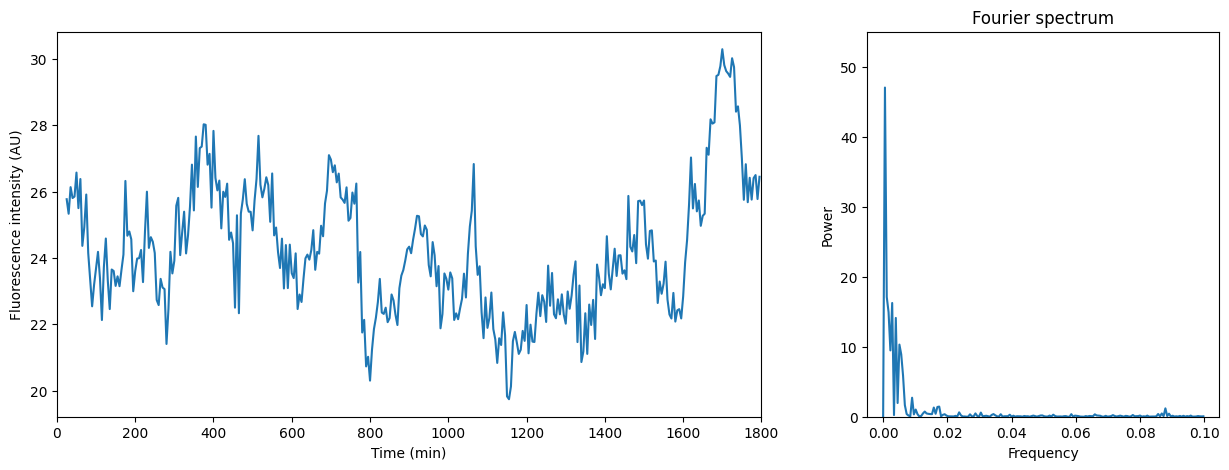
\includegraphics[width=\textwidth]{fft_raw}
   \caption{
   }
   \label{fig:analysis-filter-raw}
  \end{subfigure}

  \begin{subfigure}[htpb]{0.8\textwidth}
   \centering
   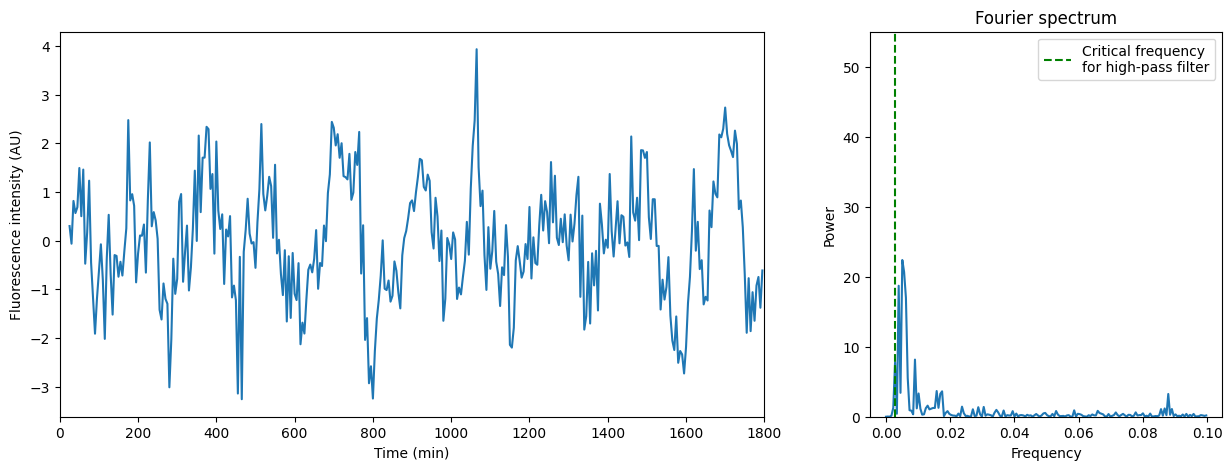
\includegraphics[width=\textwidth]{fft_butterworth}
   \caption{
   }
   \label{fig:analysis-filter-butterworth}
  \end{subfigure}

  \begin{subfigure}[htpb]{0.8\textwidth}
   \centering
   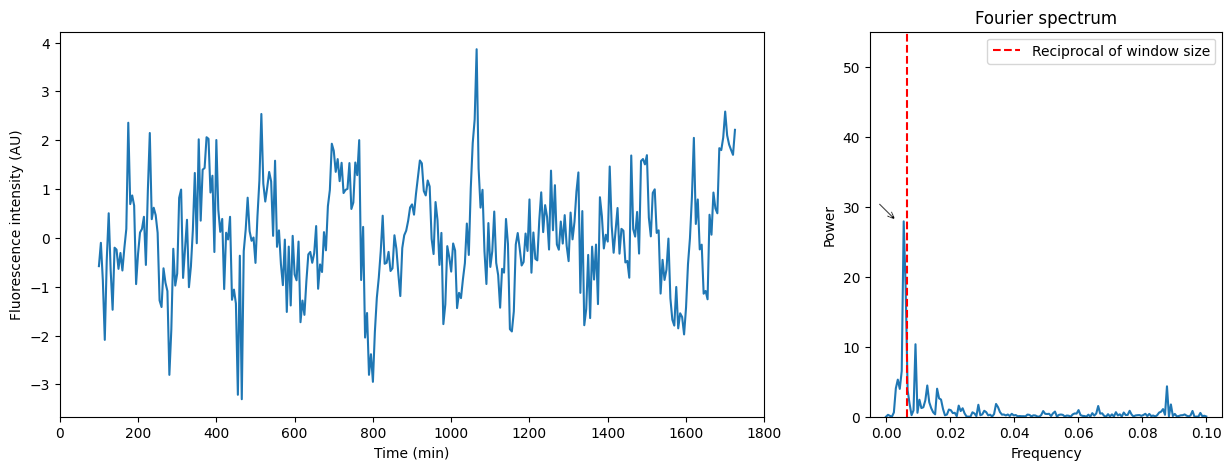
\includegraphics[width=\textwidth]{fft_slidingwindow_edit}
   \caption{
   }
   \label{fig:analysis-filter-movavg}
  \end{subfigure}

  \caption[
    Time series and Fourier spectra corresponding to
    a sample raw time series of flavin autofluorescence,
    the time series processed by a high-pass Butterworth filter, and
    the time series detrended using a moving average.
  ]{
    (Left panels) Time series and (right panels) Fourier spectra corresponding to
    \textbf{(\ref{fig:analysis-filter-raw})}
    a sample raw time series of flavin autofluorescence,
    \textbf{(\ref{fig:analysis-filter-butterworth})}
    the time series processed by a high-pass Butterworth filter with a critical frequency \SI{2.86d-3}{\minute^{-1}}, and
    \textbf{(\ref{fig:analysis-filter-movavg})}
    the time series detrended using a moving average (window size 30 time points).
    Arrow ($\searrow$) indicates artefact.
  }
  \label{fig:analysis-filter}
\end{figure}

\section{Visualising groups in the dataset}
\label{sec:analysis-clustering}

To identify structures in datasets of time series, I implemented UMAP, a dimension-reduction method, and modularity clustering, a graph-based clustering method.
Such data visualisation methods are important because the structures they show may identify differences between groups that are biologically relevant --- for example, sub-populations of oscillations with similar properties.
Previous efforts in using computational methods to identify groups in a set of biological time series include using $k$-means clustering to identify clusters of transcript cycling patterns that correspond to phases of the YMC \parencite{tuLogicYeastMetabolic2005}, development of a method to cluster featurised multivariate time series based of videos of human motion \parencite{wangStructureBasedStatisticalFeatures2007}, and using signal entropy to featurise fMRI signals followed by modularity clustering to partition the signals into brain regions.

To demonstrate the data visualisation methods, I used time series of flavin autofluorescence oscillations from one experiment with both the wild-type BY4741 strain ($n=206$) and the mutant \textit{zwf1$\Delta$} strain ($n=425$).
These time series had time points sampled every \SI{5}{\minute} in the experiment, for a total of 163 time points.
I manually labelled the time series to indicate whether they were oscillatory or not, with 142 of the 206 BY4741 time series classed as oscillatory and 224 of the 425 \textit{zwf1$\Delta$} classed as oscillatory.


\subsection{UMAP}
\label{subsec:analysis-clustering-umap}

UMAP \parencite{mcinnesUMAPUniformManifold2020} is an unsupervised dimension reduction method that can be used to visualise structure in a dataset.
Specifically, UMAP aims to find a manifold structure of the input observations and compute a low-dimensional embedding that preserves the topological structure of the manifold.
This embedding thus serves as coordinates to plot the data onto a low-dimensional space.

To evaluate whether UMAP was able to discover a structure within the BY4741 \& \textit{zwf1$\Delta$} dataset that corresponded to meaningful divisions, I featurised the time series with \textit{catch22}, then used UMAP to compute two-dimensional embeddings.
Fig.\ \ref{fig:umap-osc} demonstrates that UMAP suggested a small group of non-oscillatory time series that differed markedly from the rest ($\ast$ in figure), and a larger group that was more similar to oscillatory time series ($\ast \ast$ in figure).
In addition, Fig.\ \ref{fig:umap-strain} demonstrates that UMAP suggested that the BY4741 time series were more similar to each other.
In contrast, \textit{zwf1$\Delta$} occupied larger regions of the embedding space.
These embeddings agreed with my observation that time series from the \textit{zwf1$\Delta$} strain had a larger variety of shapes and oscillation quality than the BY4741 strain.
Thus, UMAP may have potential to separate oscillatory and non-oscillatory time series, or time series of different shapes.

\begin{figure}
  \centering
  \begin{subfigure}[t]{0.5\textwidth}
  \centering
    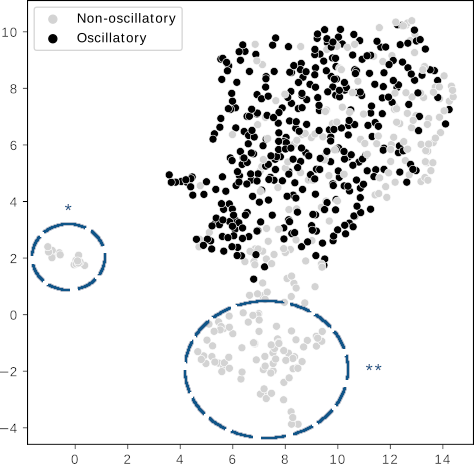
\includegraphics[width=\linewidth]{umap_single_is20016_2_edit2.png}
    \caption{
    }
    \label{fig:umap-osc}
  \end{subfigure}%
  \begin{subfigure}[t]{0.5\textwidth}
  \centering
    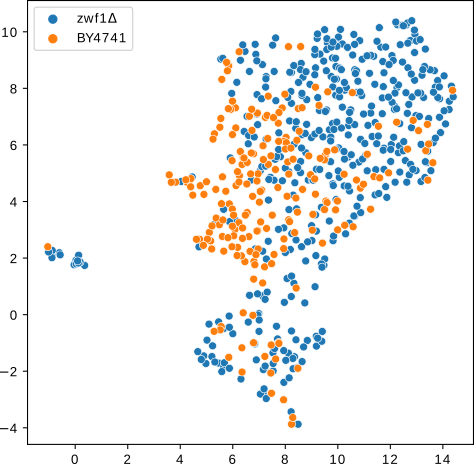
\includegraphics[width=\linewidth]{umap_single_is20016_1_edit.png}
    \caption{
    }
    \label{fig:umap-strain}
  \end{subfigure}

  \caption[
      UMAP embedding of a dataset of time series featurised using \textit{catch22}.
    ]{
      UMAP embedding ($n=5$, $\mathrm{min\_dist} = 0.5$, $d=2$, Euclidean distance as the metric) of a dataset of time series featurised using \textit{catch22}.
      Each node represents a time series, coloured either by
      \textbf{(\ref{fig:umap-osc})}
      whether each is oscillatory or not, human-labelled ($\ast$ and $\ast \ast$ indicating two groups of non-oscillatory nodes of interest), or by
      \textbf{(\ref{fig:umap-strain})}
      strain (`BY4741' or `\textit{zwf1$\Delta$}').
    }
  \label{fig:umap}
\end{figure}

To improve the visualisation, I performed a grid search of the $n$ and $\mathrm{min\_dist}$ UMAP hyperparameters (Appendix~\ref{append:analysis-umap}) to find the best combination.
Fig.\ \ref{fig:umap-gridsearch} suggests that $50 \leq n \leq 150$ and $0.25 \leq \mathrm{min\_dist} \leq 1$ resulted in a good separation between the BY4741 and \textit{zwf1$\Delta$} nodes.
In addition, non-oscillatory time series were consistently displayed into groups separate from the rest as the hyperparameters were varied.

\begin{figure}
  \centering
    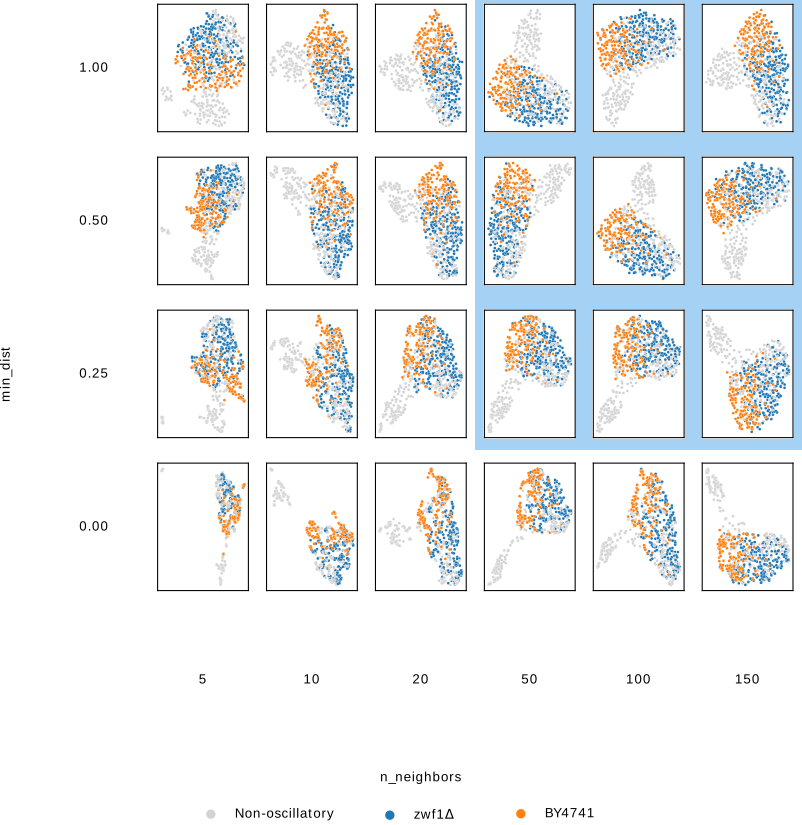
\includegraphics[width=0.9\linewidth]{umap_grid_is20016_edit3.png}
    \caption[
      Grid search of UMAP hyperparameters.
    ]{
      Grid search of UMAP hyperparameters: number of neighbours along the horizontal axis and minimum distance along the vertical axis.
      Data points are coloured according to category: grey indicates non-oscillatory time series, blue indicates oscillatory time series from \textit{zwf1$\Delta$} cells, and orange indicates oscillatory time series from BY4741 cells.
    }
  \label{fig:umap-gridsearch}
\end{figure}


\subsection{Graph-based clustering}
\label{subsec:analysis-clustering-graphclustering}

Modularity clustering is a mathematical method that partitions a graph into groups to optimise a `modularity' value, defined so that the method finds a trade-off between maximising the connections within a cluster and minimising the connections between clusters \parencite{newmanModularityCommunityStructure2006}.
This optimisation problem is computationally difficult, so approximations such as the Louvain algorithm are needed for large networks \parencite{blondelFastUnfoldingCommunities2008}, with the Leiden algorithm \parencite{traagLouvainLeidenGuaranteeing2019} subsequently developed to ensure that communities are well-connected and to provide an optimum number of communities.
Furthermore, the intrinsic scale of modularity scales with the square root of the number of connections in the network; therefore, if the network is large, there is a large resolution limit, preventing a modularity clustering algorithm from detecting small-scale structures \parencite{fortunatoResolutionLimitCommunity2007,traagNarrowScopeResolutionlimitfree2011}.
To remedy this, algorithms that implement a resolution parameter ($\gamma$), were devised; the value of this parameter thus controls the scale at which communities are detected \parencite{reichardtDetectingFuzzyCommunity2004,kumpulaLimitedResolutionComplex2007}.

To assess the performance of a graph-based clustering method in identifying clusters in time series data, I represented a dataset of time series as a graph before using modularity clustering to identify clusters.
Fig.\ \ref{fig:analysis-clustering-modclust} illustrates this process, specifically:
\begin{enumerate}
  \item \emph{Constructing a graph representation:}
        Each time series was represented as a vector of features in $n$-dimensional space, where $n$ is the length of the vector.
        Here, I represented each time series with a vector of 22 features using \textit{catch22}.
        The cosine distances between each pair of vector was computed, and became the edge weights of a complete graph with each time series as a node.
  \item \emph{Pruning:}
        The complete graph was pruned by deleting edges, so that each node was connected to at least the $k$ nearest neighbours.
        I used $k=10$.
  \item \emph{Modularity clustering:}
        Modularity clustering was performed on the graph to partition the pruned graph into communities.
        In this step, I used the constant Potts model \parencite{traagNarrowScopeResolutionlimitfree2011} and the Leiden algorithm \parencite{traagLouvainLeidenGuaranteeing2019}.
\end{enumerate}

\begin{figure}
  \centering
  \begin{subfigure}[t]{0.5\textwidth}
  \centering
    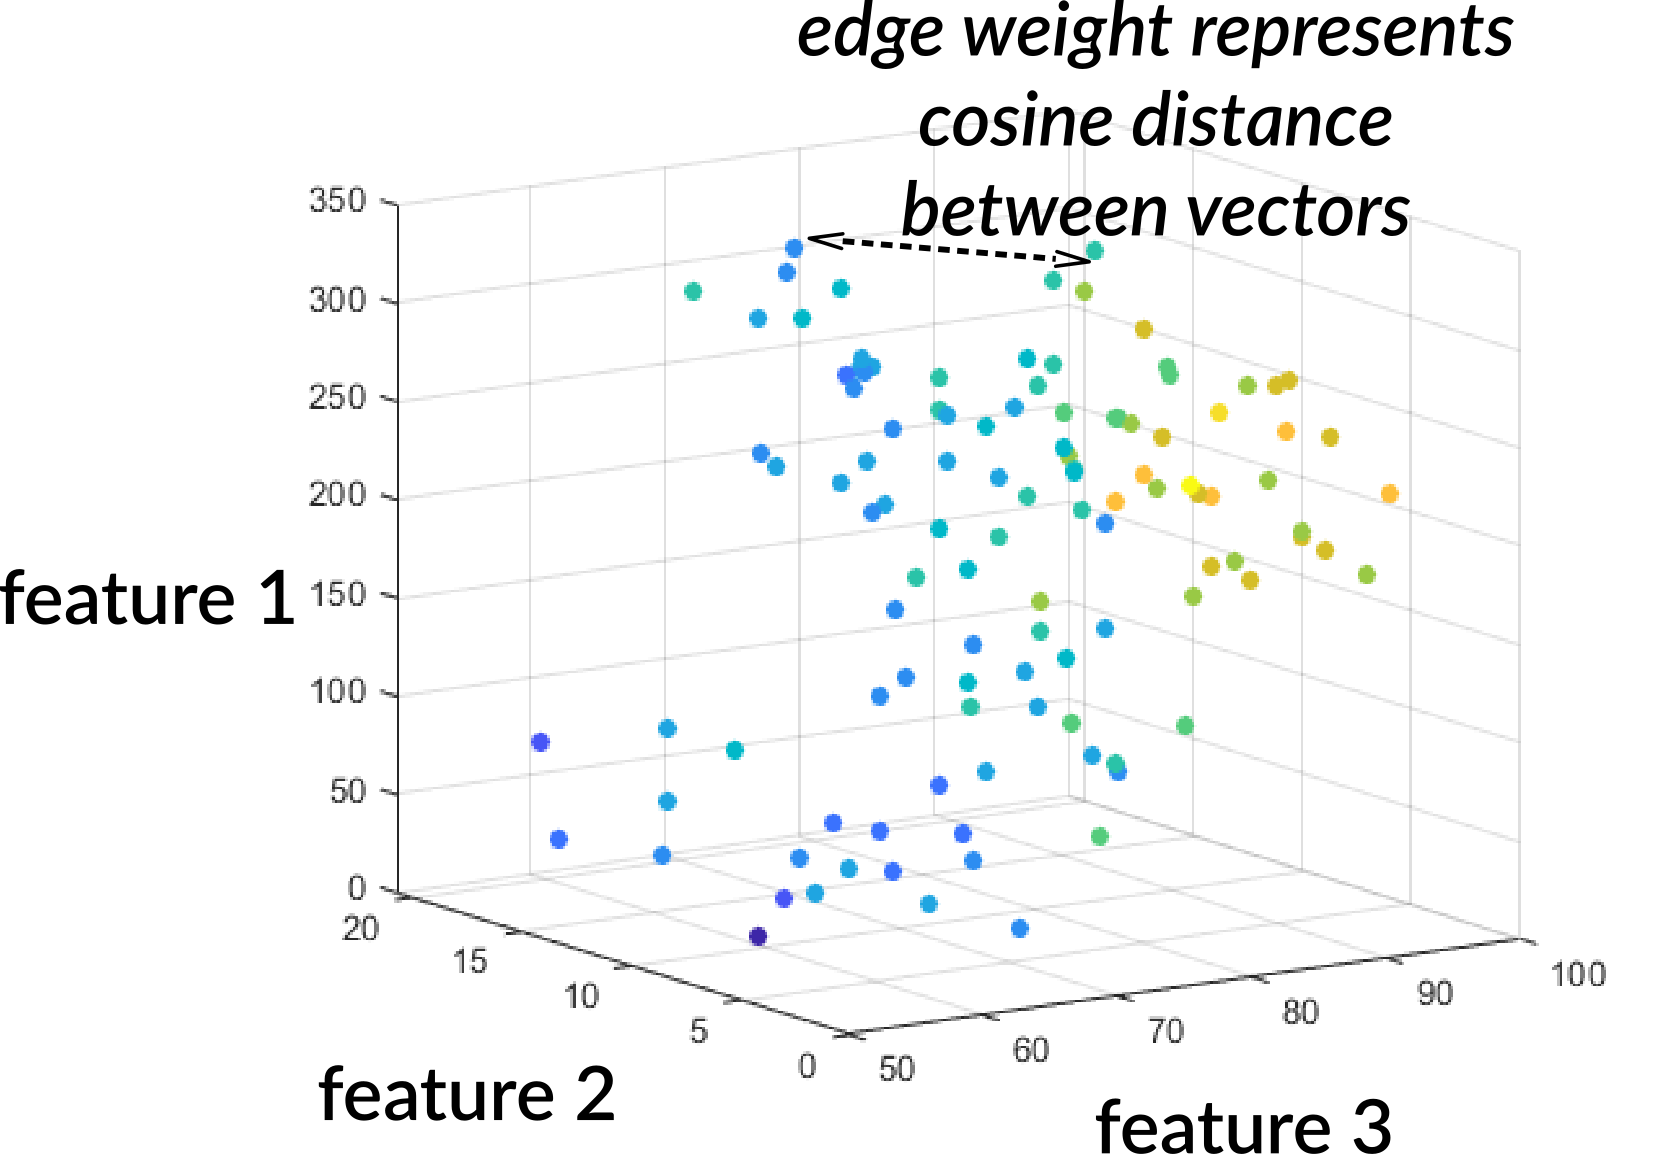
\includegraphics[width=\linewidth]{graph_representation}
    \caption{
    }
    \label{fig:analysis-clustering-modclust-graph}
  \end{subfigure}

  \begin{subfigure}[t]{0.6\textwidth}
  \centering
    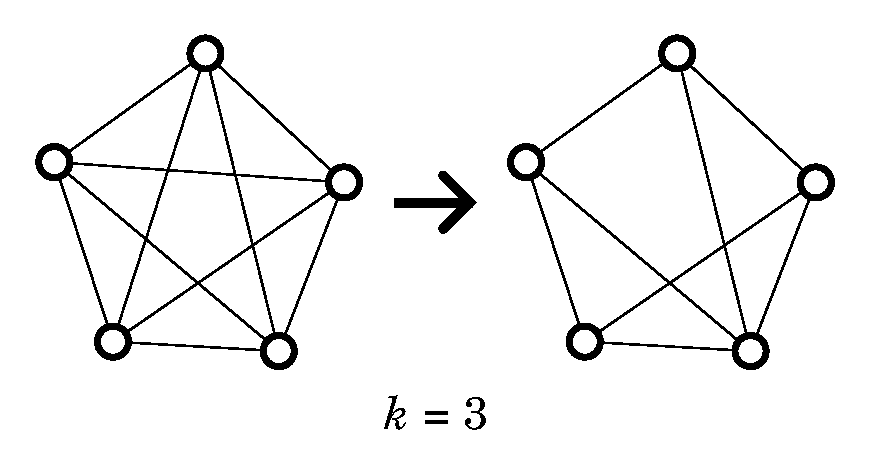
\includegraphics[width=\linewidth]{pruning}
    \caption{
    }
    \label{fig:analysis-clustering-modclust-prune}
  \end{subfigure}%
  \begin{subfigure}[t]{0.4\textwidth}
  \centering
    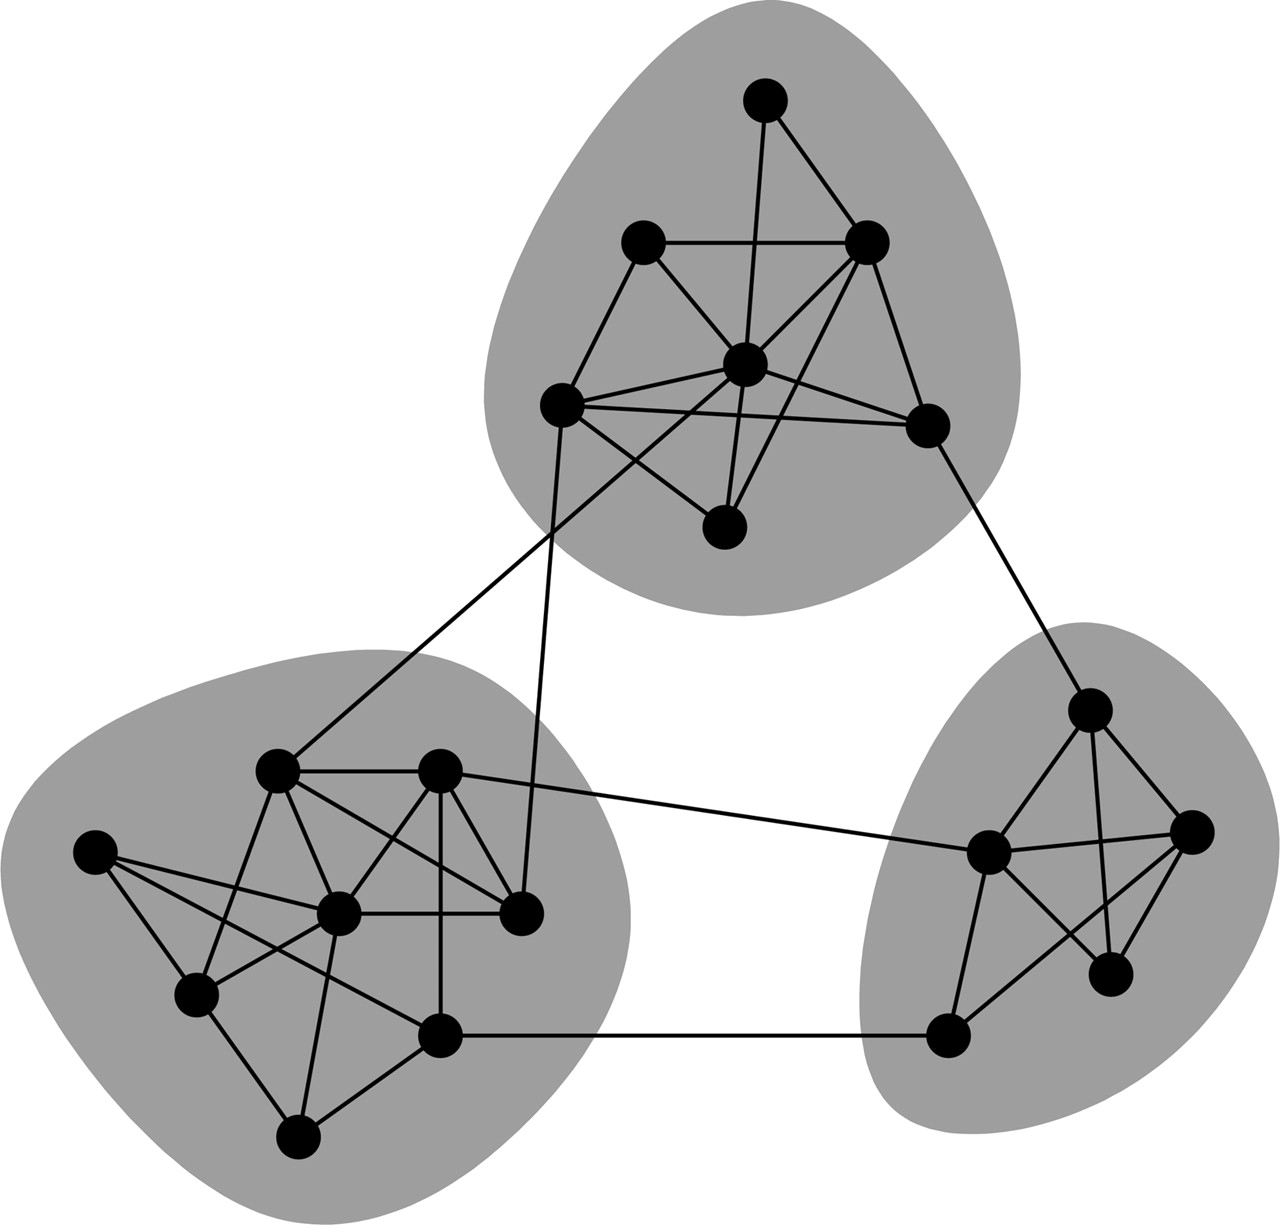
\includegraphics[width=\linewidth]{newmanModularityCommunityStructure2006_1}
    \caption{
    }
    \label{fig:analysis-clustering-modclust-modclust}
  \end{subfigure}

  \caption[
    Process of preparing a dataset of time series for modularity clustering.
  ]{
    Process of preparing a dataset of time series for modularity clustering.
    \textbf{(\ref{fig:analysis-clustering-modclust-graph})}
    Constructing a graph representation: each time series was featurised and the cosine distances in feature space became edge weights.
    \textbf{(\ref{fig:analysis-clustering-modclust-prune})}
    Pruning the complete graph so that each node had at least the $k$ nearest neighbours.
    \textbf{(\ref{fig:analysis-clustering-modclust-modclust})}
    Modularity clustering, using the Leiden algorithm \parencite{traagLouvainLeidenGuaranteeing2019}, to identify communities.
    \ref{fig:analysis-clustering-modclust-modclust} adapted from \textcite{newmanModularityCommunityStructure2006}.
    In all subfigures, data are synthetic and only serve to illustrate the process.
  }
  \label{fig:analysis-clustering-modclust}
\end{figure}

Fig.\ \ref{fig:graphclustering-combined} shows that construction of a pruned graph based on similarities between time series highlights two groups of non-oscillatory time series.
Subsequently, Figs.\ \ref{fig:graphclustering-cpm_00p010}--\ref{fig:graphclustering-cpm_00p030} show that the resolution parameter ($\gamma$) controls the number of communities detected.
Non-oscillatory time series were assigned to a separate group when $\gamma = 0.01$, and the two sub-groups of non-oscillatory time series were separated when $\gamma = 0.02$; however, when $\gamma = 0.03$, the divisions changed.
The Leiden algorithm \parencite{traagLouvainLeidenGuaranteeing2019} suggested 10 as the optimal number of communities, which was realised by $\gamma = 0.02$.
For all $\gamma$ values, modularity clustering was able to further show communities among the oscillatory time series.

\begin{figure}[htbp]
  \centering
  \begin{subfigure}[t]{0.5\textwidth}
  \centering
    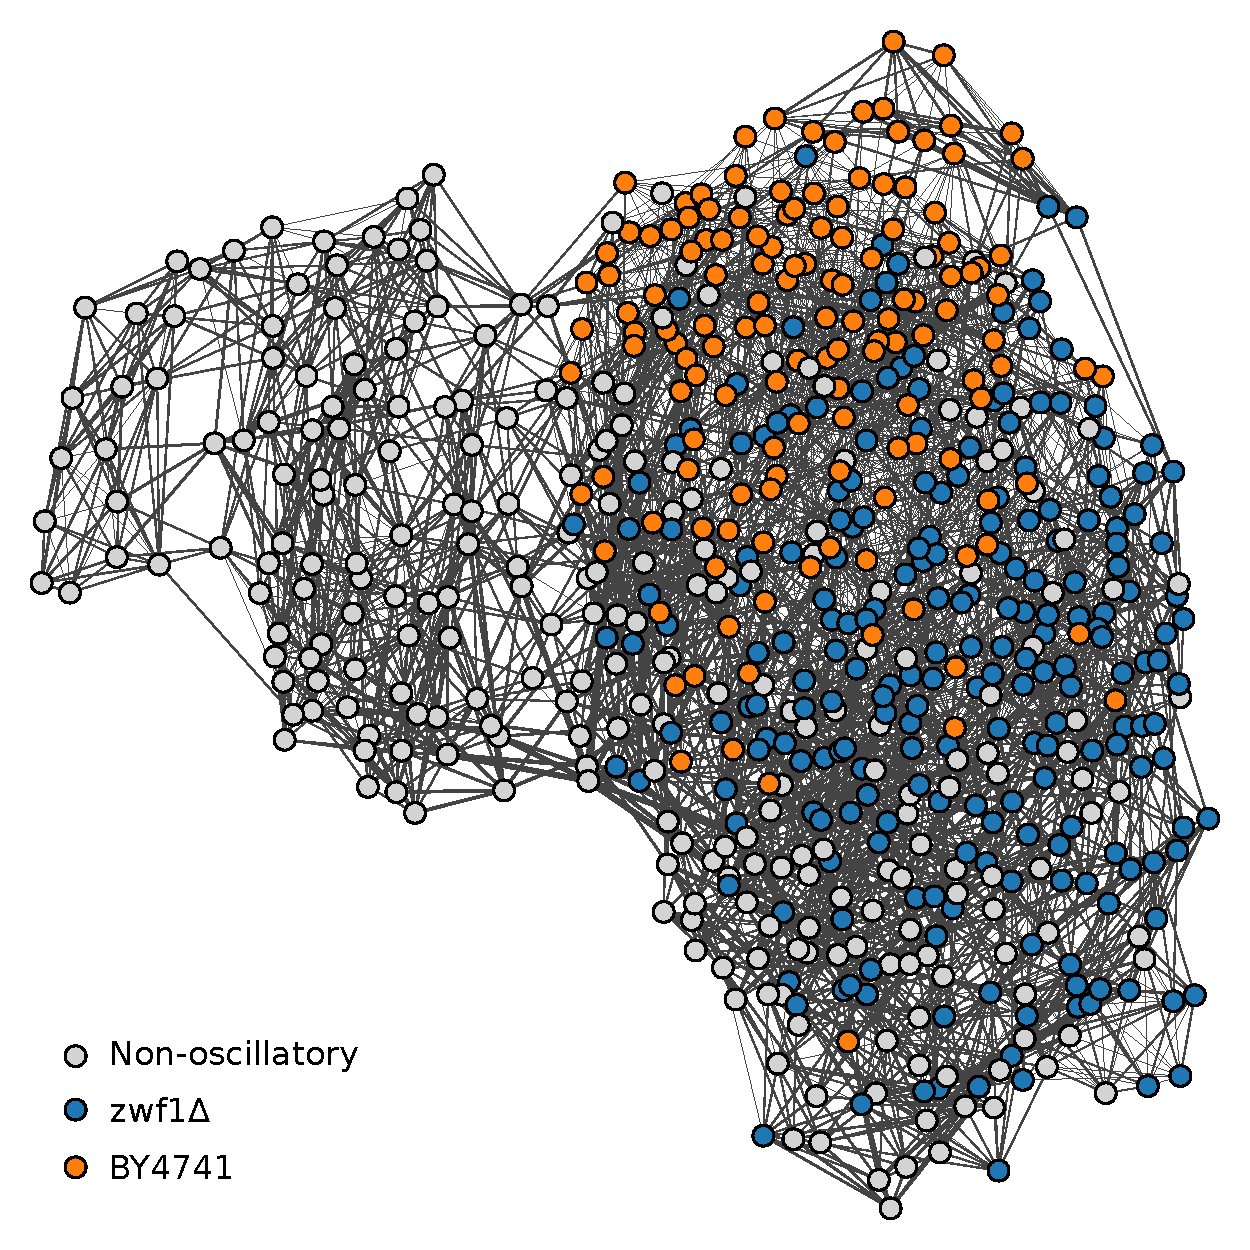
\includegraphics[width=\linewidth]{graphclust_combined_is20016_edit1.pdf}
    \caption{
    }
    \label{fig:graphclustering-combined}
  \end{subfigure}

  % \begin{subfigure}[t]{0.5\textwidth}
  % \centering
  %   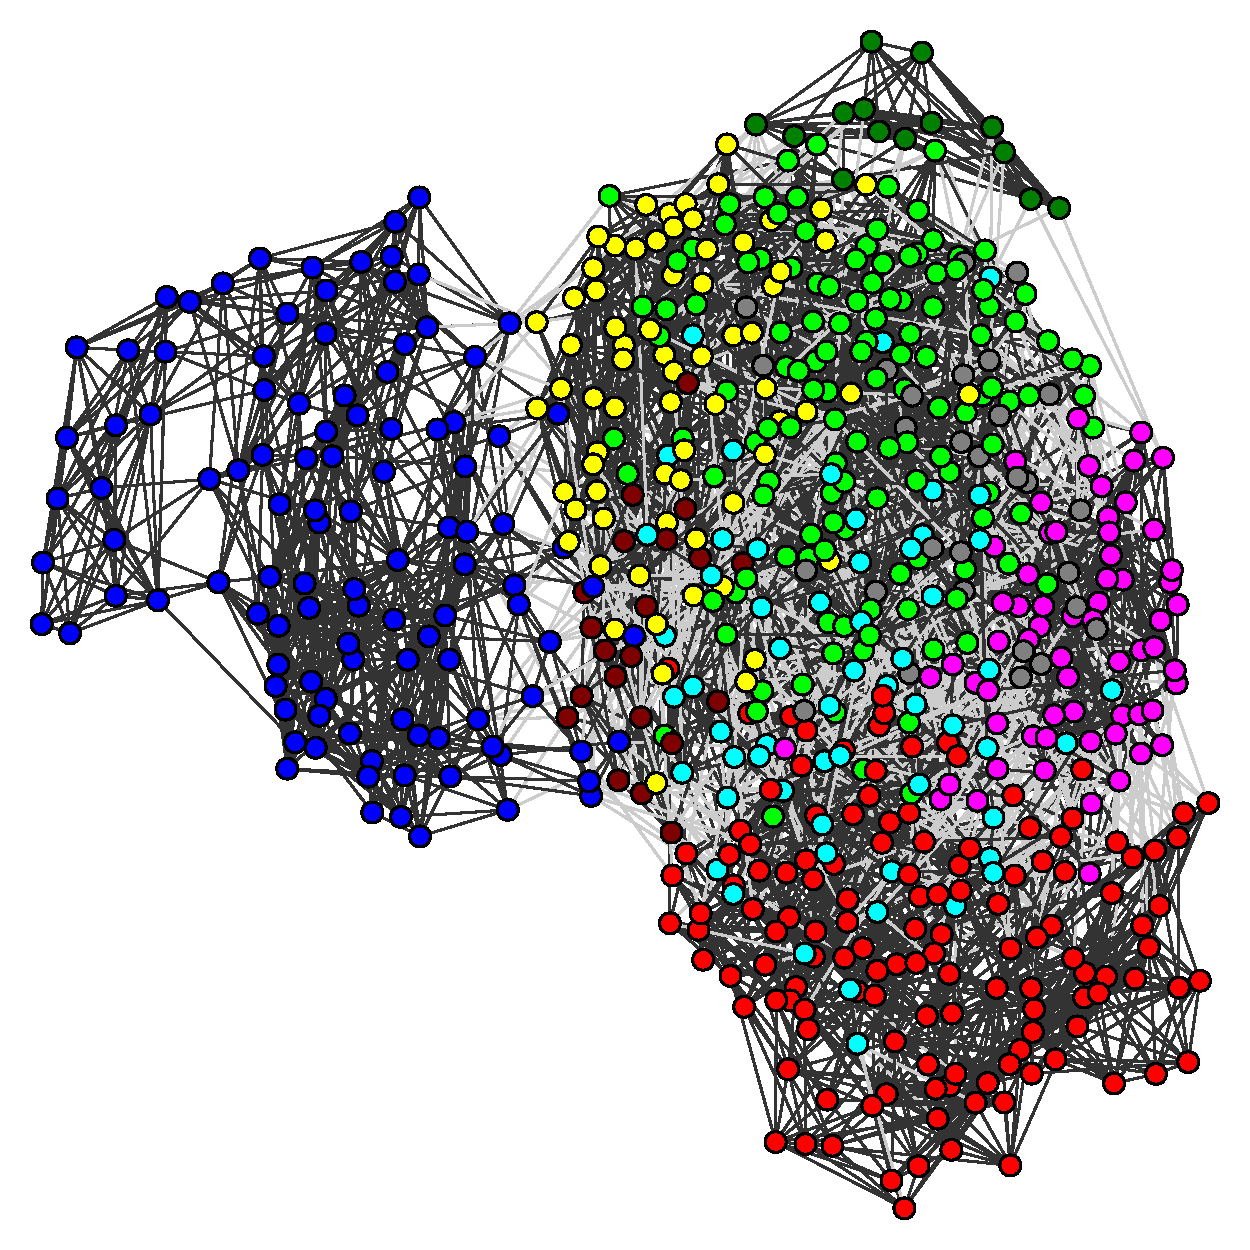
\includegraphics[width=\linewidth]{graphclust_leiden_is20016.pdf}
  %   \caption{
  %   }
  %   \label{fig:graphclustering-leiden}
  % \end{subfigure}

  \begin{subfigure}[t]{0.33\textwidth}
  \centering
    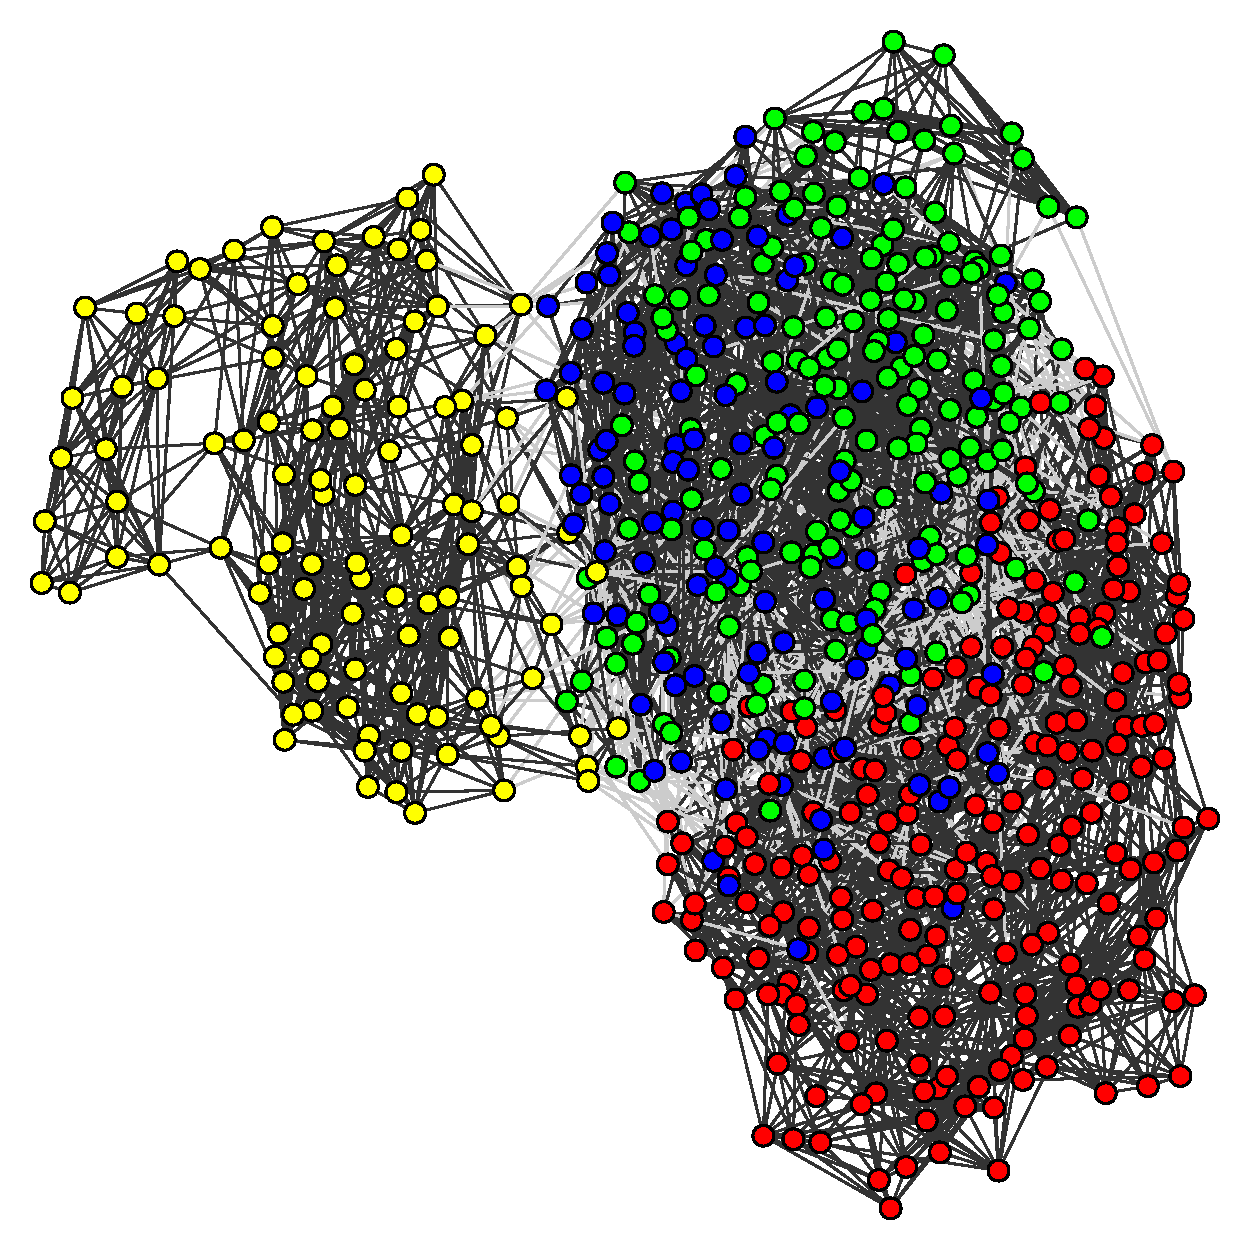
\includegraphics[width=\linewidth]{graphclust_cpm_00p010_is20016.pdf}
    \caption{
    }
    \label{fig:graphclustering-cpm_00p010}
  \end{subfigure}%
  \begin{subfigure}[t]{0.33\textwidth}
  \centering
    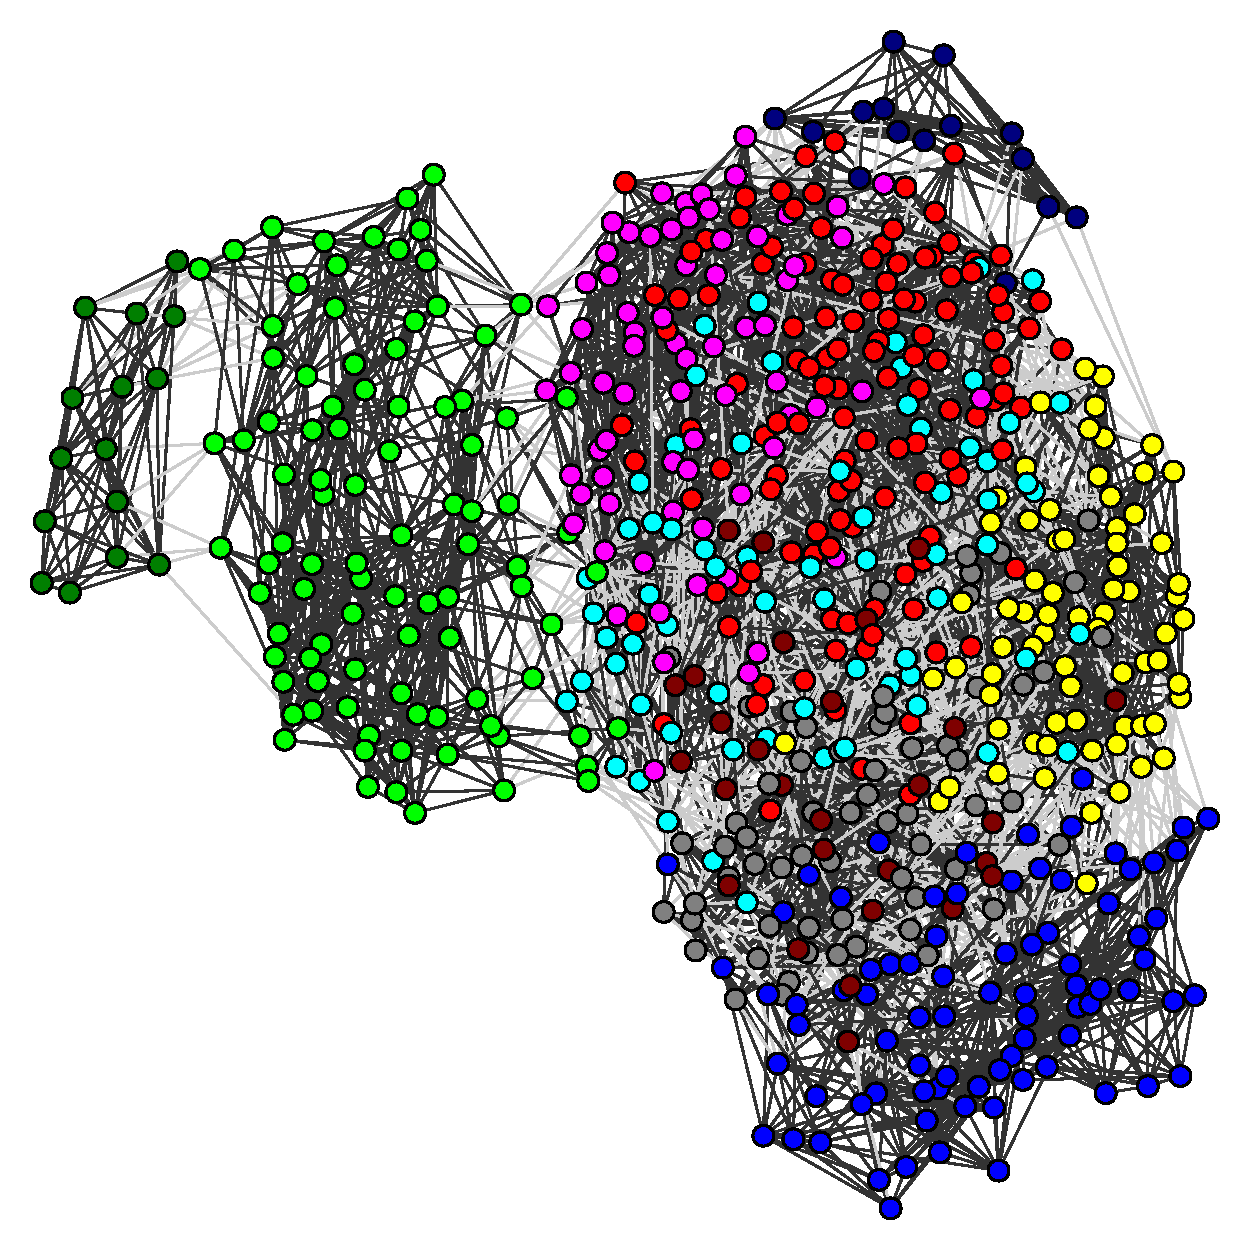
\includegraphics[width=\linewidth]{graphclust_cpm_00p020_is20016.pdf}
    \caption{
    }
    \label{fig:graphclustering-cpm_00p020}
  \end{subfigure}%
  \begin{subfigure}[t]{0.33\textwidth}
  \centering
    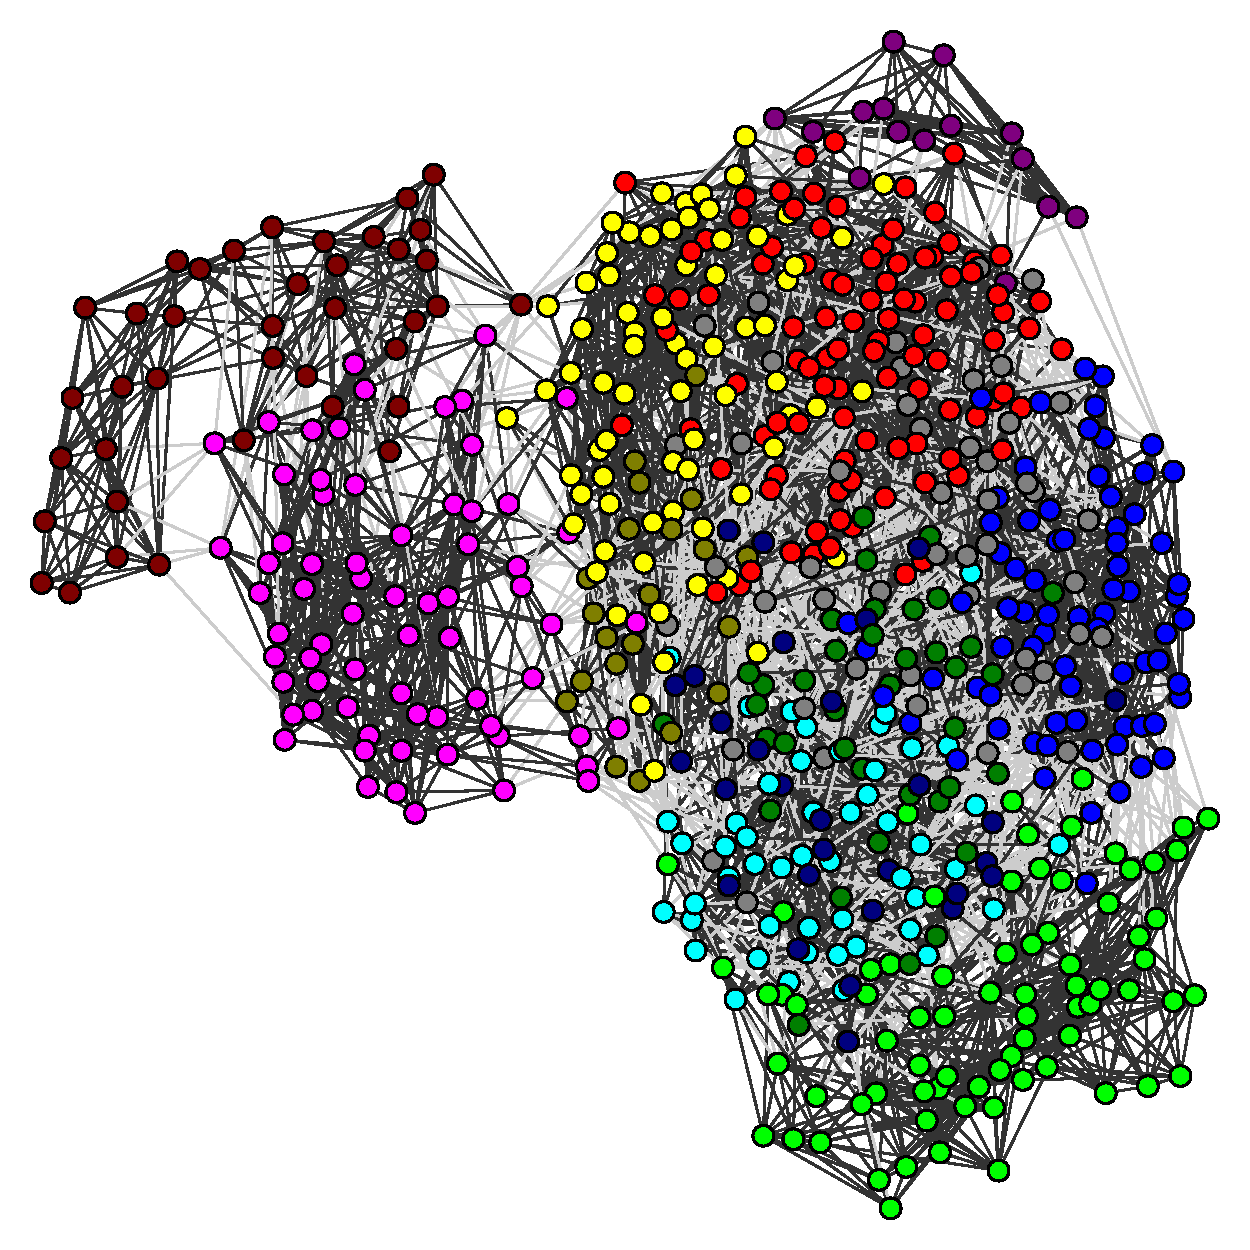
\includegraphics[width=\linewidth]{graphclust_cpm_00p030_is20016.pdf}
    \caption{
    }
    \label{fig:graphclustering-cpm_00p030}
  \end{subfigure}

  \caption[
    Pruned graph of BY4741 and \textit{zwf1$\Delta$} time series from the same experiment.
  ]{
    Pruned graph of BY4741 and \textit{zwf1$\Delta$} time series from the same experiment.
    \textbf{(\ref{fig:graphclustering-combined})}
    Nodes coloured by group: grey, non-oscillatory; blue, oscillatory \textit{zwf1$\Delta$}; orange, oscillatory BY4741.
    Thickness of edges represent edge weights, scaled by similarity found by cosine distances.
    % \textbf{(\ref{fig:graphclustering-leiden})}
    % Nodes coloured by community (out of 10) as optimised by the Leiden algorithm.
    % Edges within a community are in black, while edges between communities are in light grey.
    Additionally, nodes coloured by community as found by the constant Potts model \parencite{traagNarrowScopeResolutionlimitfree2011} as the resolution parameter ($\gamma$) was varied:
    \textbf{(\ref{fig:graphclustering-cpm_00p010})} $\gamma = 0.01$ (4 communities),
    \textbf{(\ref{fig:graphclustering-cpm_00p020})} $\gamma = 0.02$ (10 communities), and
    \textbf{(\ref{fig:graphclustering-cpm_00p030})} $\gamma = 0.03$ (12 communities).
  }
  \label{fig:graphclustering}
\end{figure}

However, such communities did not divide along the division between BY4741 and \textit{zwf1$\Delta$} cells, suggesting that time series features alone were not able to divide these two strains.
This agreed with my observation that some oscillatory \textit{zwf1$\Delta$} time series resembled BY4741 time series (Fig.\ \ref{fig:analysis-sample-zwf1}).

\begin{figure}[hb!]
  \centering
  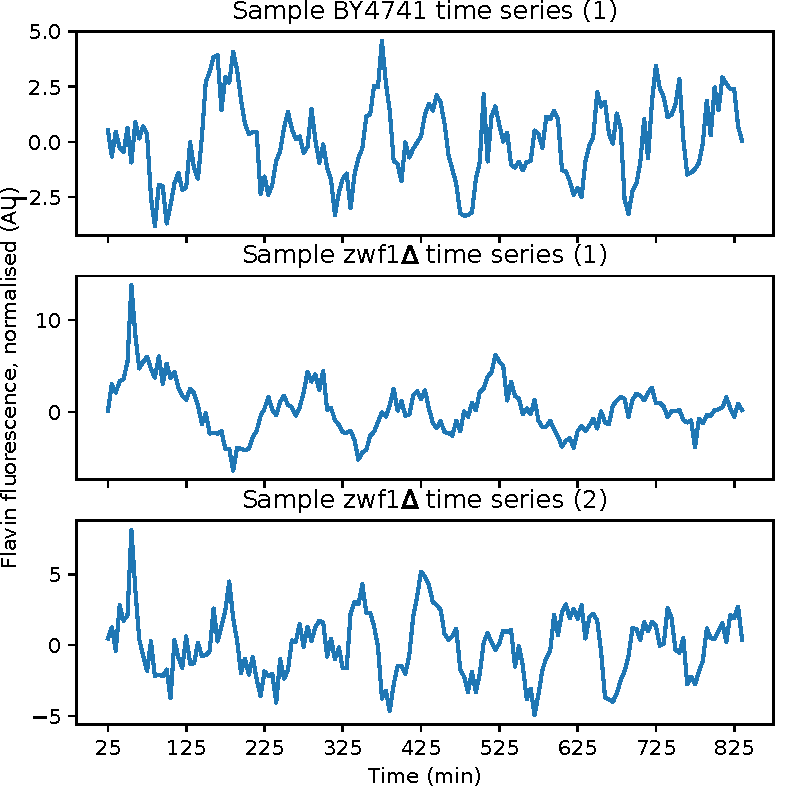
\includegraphics[width=0.6\linewidth]{sample_ts_zwf1.pdf}

  \caption[
    Sample time series from BY4741 and \textit{zwf1$\Delta$} cells.
  ]{
    Sample time series from BY4741 and \textit{zwf1$\Delta$} cells.
    \textit{zwf1$\Delta$} sample 1 does not resemble the BY4741 sample, while \textit{zwf1$\Delta$} sample 2 does.
  }
  \label{fig:analysis-sample-zwf1}
\end{figure}

% PLOT AVERAGE TIME SERIES FROM EACH COMMUNITY?

In sum, the general agreement between UMAP and modularity clustering shows that the BY4741 \& \textit{zwf1$\Delta$} dataset had internal structure defined by rhythmicity of time series.
However, it was not clear from UMAP whether there were sub-populations among the BY4741 and \textit{zwf1$\Delta$} time series whose members exhibit similar types of oscillations.
In contrast, while modularity clustering suggests that such sub-populations can be found based on connectivity between nodes, the number of sub-populations depends on the value of a resolution parameter.


\section{Detection of rhythmicity}
\label{sec:analysis-classification}

To identify metabolic cycles from flavin autofluorescence signals, it is important to have a systematic method to determine whether a time series is oscillatory.
To determine the time series classification method that is most appropriate for my data, I compared a spectral method, a model-fitting method, and a machine learning method.


\subsection{Spectral methods}
\label{subsec:analysis-classification-spectral}

In order to classify oscillatory and non-oscillatory time series, I modified a classifier based on a spectral method that included a statistical test (Methods Section~\ref{subsec:methods-computational-periodogram}).
This classifier was based on \textcite{glynnDetectingPeriodicPatterns2006}, which described a method that employed the peak power from the Lomb-Scargle periodogram \parencite{lombLeastsquaresFrequencyAnalysis1976} to rank time series by the quality of oscillation and to perform a statistical test to determine whether a time series is oscillatory or non-oscillatory \parencite{scargleStudiesAstronomicalTime1982}, as shown by Eqs.\ \ref{eq:lsp-pval}--\ref{eq:lsp-khat}.

Figs.\ \ref{fig:glynn-best}--\ref{fig:glynn-worst} suggest that the best- and worst-ranked time series according to the quality of their oscillatory signals conformed to subjective judgements of quality.
Highest-ranked time series resembled sinusoids and therefore led to periodograms with a strong power corresponding to the frequency of the sinusoid that would model the time series.
Conversely, lowest-ranked time series resembled white noise and led to periodograms with power equally spread across all frequencies, thus bringing down the height of the highest peak.
However, some time series with irregular oscillations based on visual inspection (Fig.\ \ref{fig:glynn-best}; ranks 2, 3) were given higher ranks than those with more regular oscillations based on visual inspection, thus calling into question the reliability of the ranking method.

\begin{figure}[p]
  \centering
  \begin{subfigure}[t]{0.65\textwidth}
  \centering
    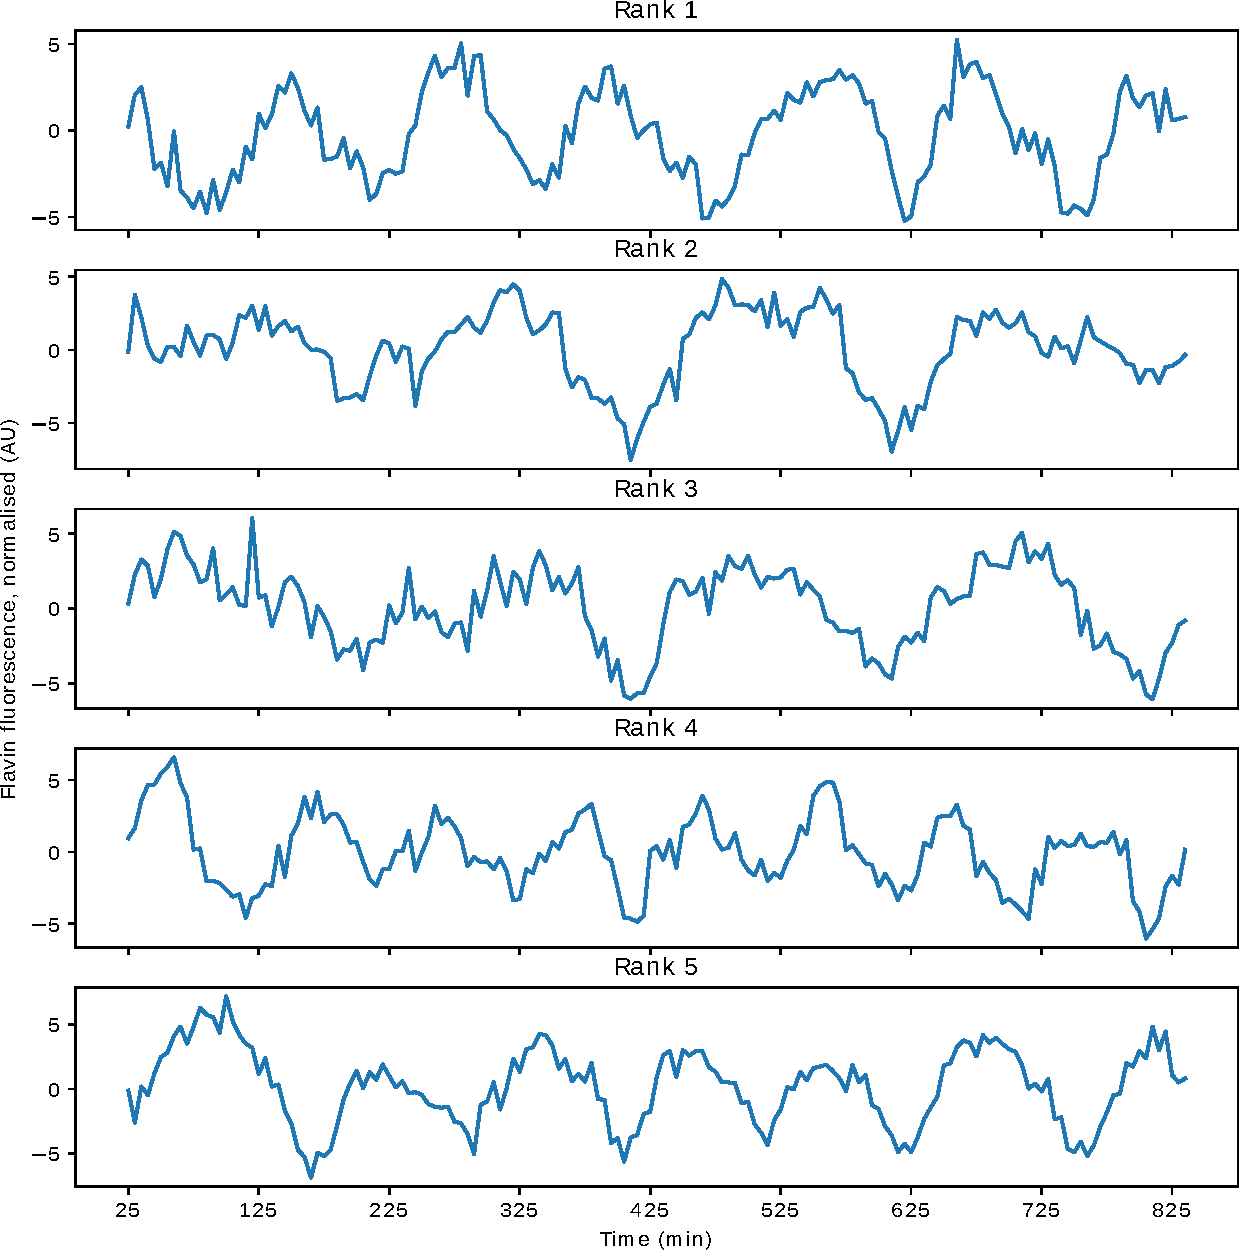
\includegraphics[width=\linewidth]{glynn_is20016_1_edit.pdf}
    \caption{
    }
    \label{fig:glynn-best-ts}
  \end{subfigure}%
  \begin{subfigure}[t]{0.35\textwidth}
  \centering
    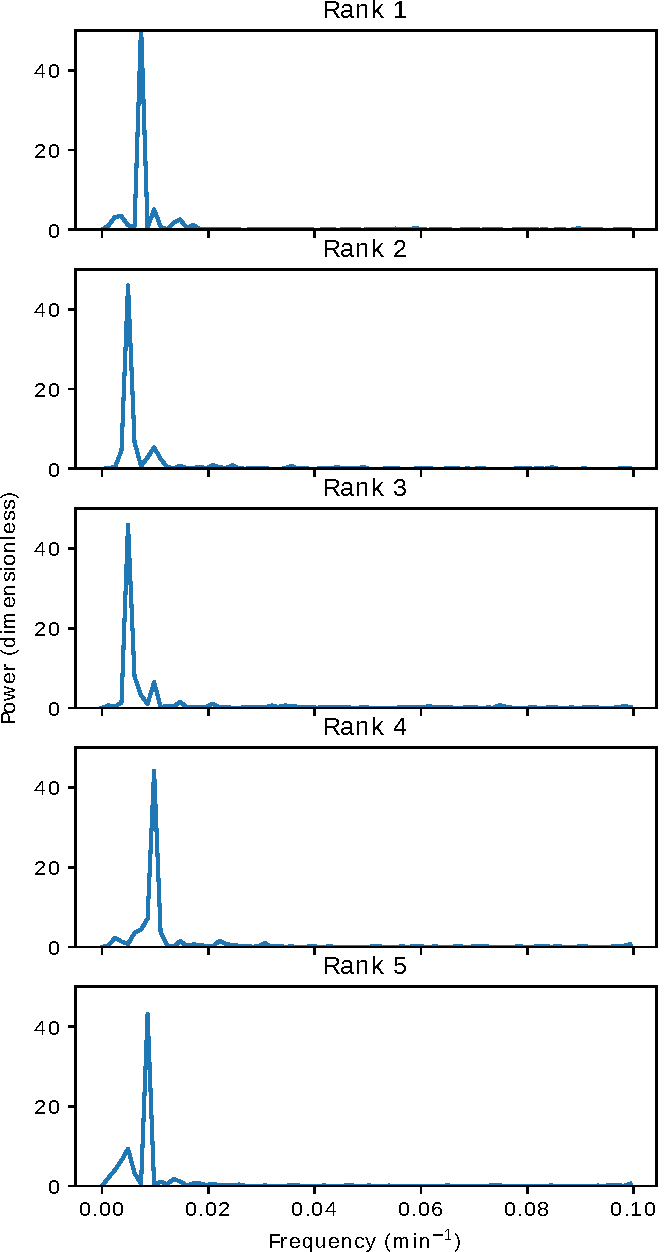
\includegraphics[width=\linewidth]{glynn_is20016_2_edit.pdf}
    \caption{
    }
    \label{fig:glynn-best-ps}
  \end{subfigure}

  \caption[
    Best five time series in the \textit{zwf1$\Delta$} dataset and
    their periodograms,
    ranked by the quality of oscillation based on the maximum power in the periodogram \parencite{glynnDetectingPeriodicPatterns2006}
  ]{
    \textbf{(\ref{fig:glynn-best-ts})}
    Best five time series in the \textit{zwf1$\Delta$} dataset and
    \textbf{(\ref{fig:glynn-best-ps})}
    their periodograms,
    ranked by the quality of oscillation based on the maximum power in the periodogram \parencite{glynnDetectingPeriodicPatterns2006}.
  }
  \label{fig:glynn-best}
\end{figure}

\begin{figure}[p]
  \centering
  \begin{subfigure}[t]{0.65\textwidth}
  \centering
    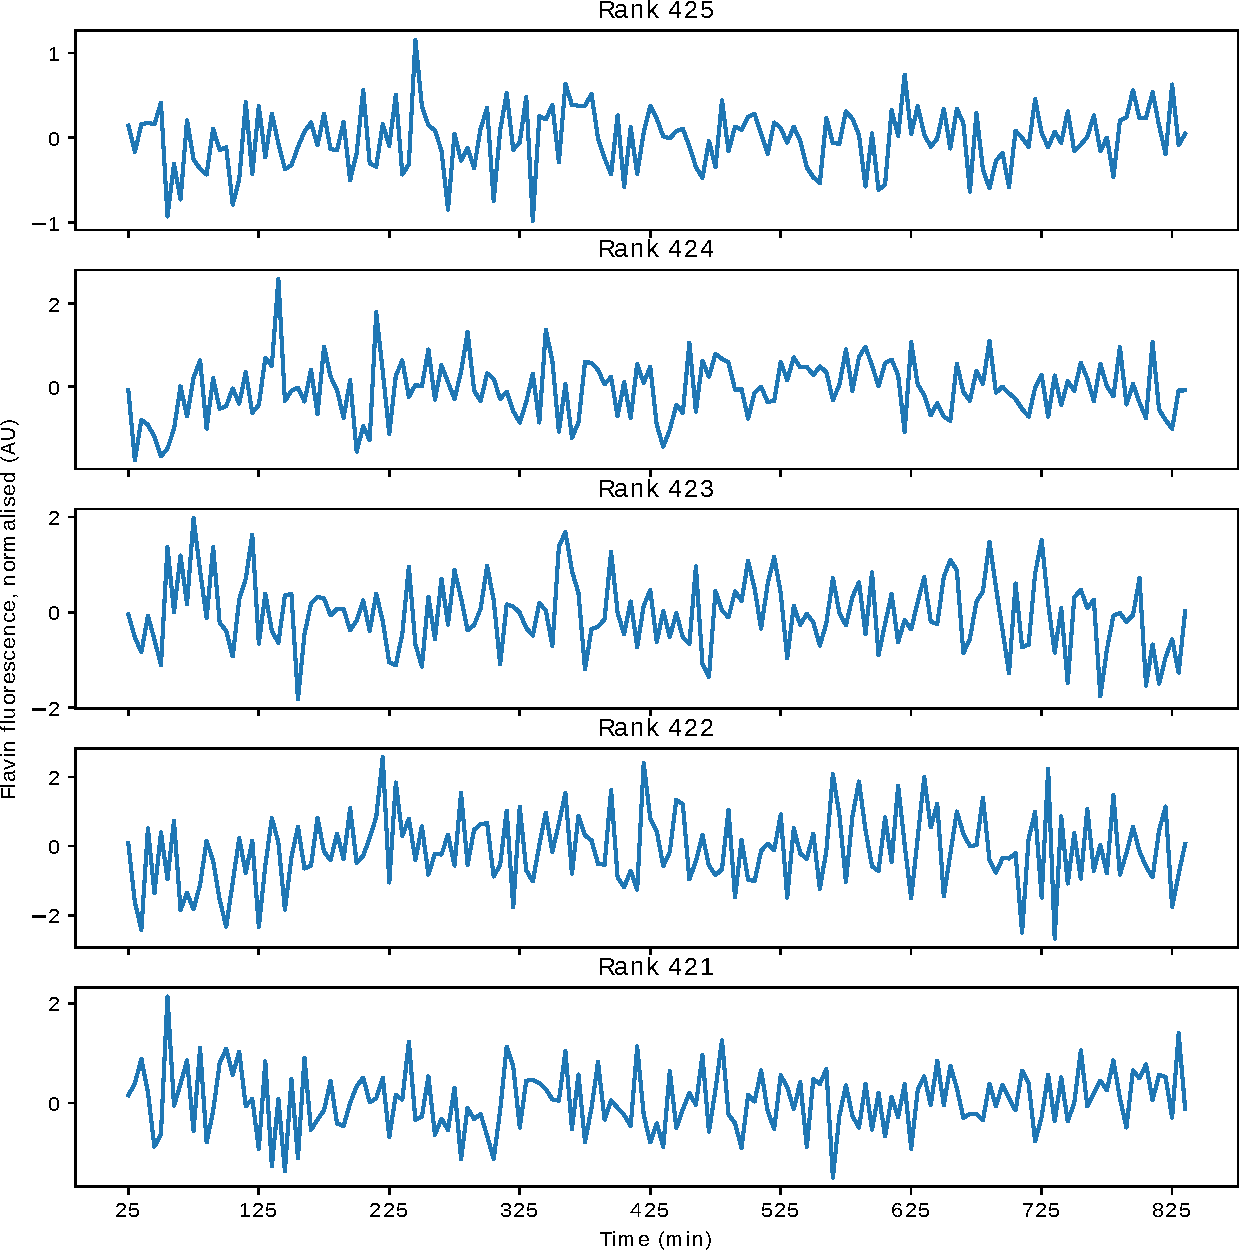
\includegraphics[width=\linewidth]{glynn_is20016_3_edit.pdf}
    \caption{
    }
    \label{fig:glynn-worst-ts}
  \end{subfigure}%
  \begin{subfigure}[t]{0.35\textwidth}
  \centering
    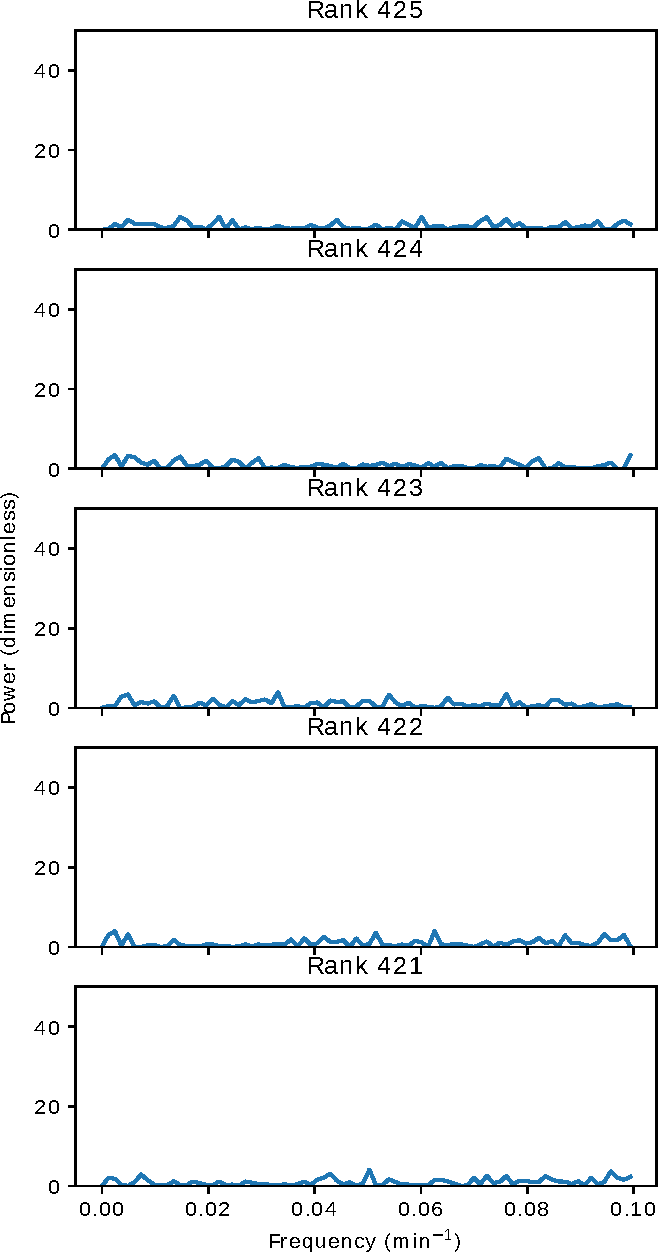
\includegraphics[width=\linewidth]{glynn_is20016_4_edit.pdf}
    \caption{
    }
    \label{fig:glynn-worst-ps}
  \end{subfigure}

  \caption[
    Worst five time series in the \textit{zwf1$\Delta$} dataset and
    their periodograms,
    ranked by the quality of oscillation based on the maximum power in the periodogram \parencite{glynnDetectingPeriodicPatterns2006}
  ]{
    \textbf{(\ref{fig:glynn-worst-ts})}
    Worst five time series in the \textit{zwf1$\Delta$} dataset and
    \textbf{(\ref{fig:glynn-worst-ps})}
    their periodograms,
    ranked by the quality of oscillation based on the maximum power in the periodogram \parencite{glynnDetectingPeriodicPatterns2006}.
  }
  \label{fig:glynn-worst}
\end{figure}

To detect rhythmicity in one time series, \textcite{glynnDetectingPeriodicPatterns2006} calculates the probability of the null hypothesis that a peak in the periodogram occurs due to chance.
When extended across a population of time series, rhythmicity detection by this method thus becomes a task of testing multiple hypotheses.
\textcite{glynnDetectingPeriodicPatterns2006} thus proposed controlling the false discovery rate, defined as the proportion of cases in which the null hypothesis is true among all hypotheses in which the test is declared significant (see Methods, Section~\ref{subsec:methods-computational-periodogram}, specifically Eq.\ \ref{eq:lsp-khat}).
Controlling the false discovery rate thus controls the expected proportion of oscillations that are classified as oscillatory.

To assess the performance of this method as a classifier for rhythmicity detection, Fig.\ \ref{fig:glynn-roc} shows the receiver operating characteristic (ROC) curve, created as the false discovery rate was varied.
The area under the ROC curve (0.762) suggests that the classifier performed modestly well, especially for a large ($n=425$) dataset of time series with a large variety of quality of oscillations.

\begin{figure}[hb!]
  \centering
  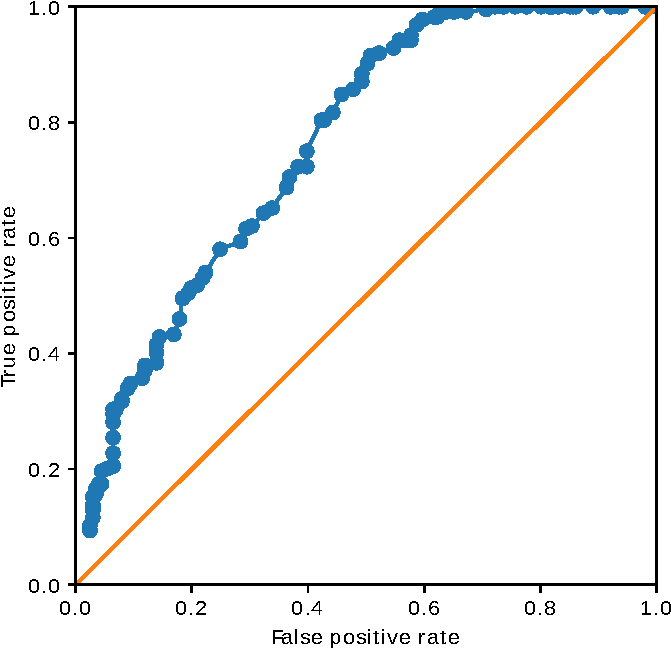
\includegraphics[width=0.5\textwidth]{glynn_is20016_5_edit.pdf}
  \caption[
    ROC curve of classifier based on \textcite{glynnDetectingPeriodicPatterns2006}.
  ]{
    ROC curve of classifier based on \textcite{glynnDetectingPeriodicPatterns2006} as the false discovery rate was varied.
    The true positive rate and false positive rates were computed based on the manual labels of the \textit{zwf1$\Delta$} dataset.
  }
  \label{fig:glynn-roc}
\end{figure}


\subsection{Model fitting}
\label{subsec:analysis-classification-ar}

To assess the performance of a time series classification method based on the autoregressive model, I implemented the method described by \textcite{jiaFrequencyDomainAnalysis2020}, used to characterise synthetic time series of stochastic, oscillatory gene expression in a dividing cell.
In the implementation of the autoregressive model used by \textcite{jiaFrequencyDomainAnalysis2020}, each data point was expressed as a linear combination of a number of data points that precede it, and model parameters led to an analytical solution for the periodogram, thus giving an advantage over the low-resolution Fourier spectrum (Methods Section~\ref{subsec:methods-computational-ar}).
The resulting power spectra fell into four categories, one of which corresponded to a lack of oscillations, characterised by an absence of a local maximum in the power spectrum (Fig.\ \ref{fig:analysis-ar-classification}).
This method thus allows computing the frequency of the oscillation from the location of the peak in the periodogram and quality of the oscillation from the height of the peak.

\begin{figure}[b!]
  \centering
  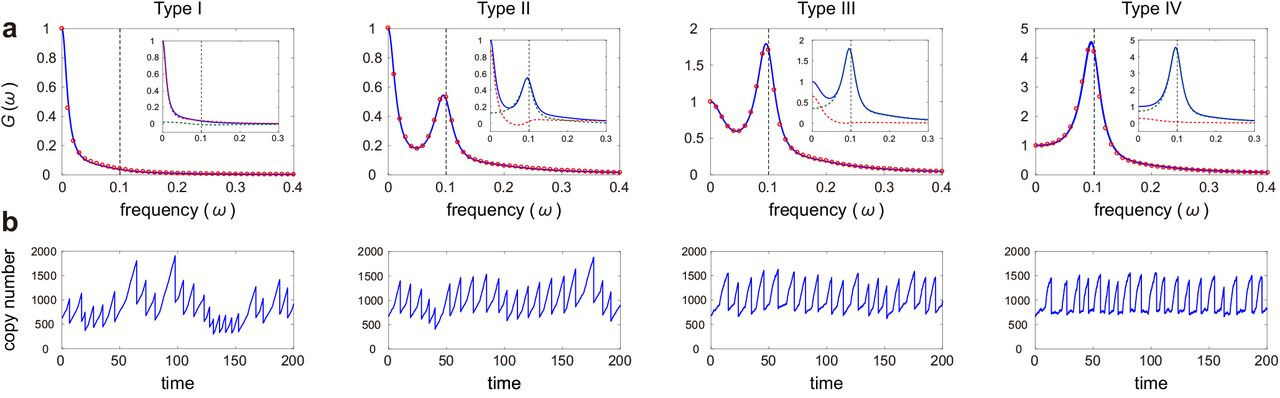
\includegraphics[width=1.0\textwidth]{jiaFrequencyDomainAnalysis2020_2ab_adapted}
  \caption[
    Power spectra analytically derived from fitting an autoregressive model to time series can be divided into four types.
  ]{
    Power spectra (a) analytically derived from fitting an autoregressive model to time series (b) can be divided into four types.
    Type I lacks a local maximum and is denoted as lacking oscillations.
    Figure adapted from \textcite{jiaFrequencyDomainAnalysis2020}.
  }
  \label{fig:analysis-ar-classification}
\end{figure}

\pagebreak

Fig.\ \ref{fig:analysis-ar} shows that the autoregressive model was able to correctly identify a time series as oscillatory at a period of \SI{75.2}{\minute}, as evidenced by the location of a peak in the periodogram that the model predicted.

\begin{figure}
  \centering
  \begin{subfigure}[htpb]{0.6\textwidth}
   \centering
   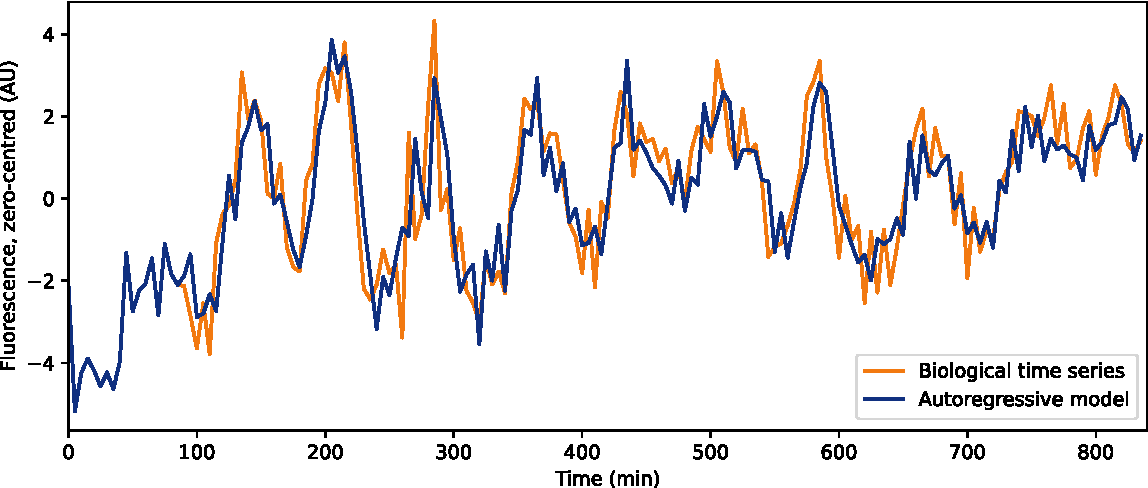
\includegraphics[width=\textwidth]{timeseries_example_for_ar_edit}
   \caption{
   }
   \label{fig:analysis-ar-timeseries}
  \end{subfigure}%
  \begin{subfigure}[htpb]{0.4\textwidth}
   \centering
   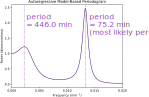
\includegraphics[width=\textwidth]{ar}
   \caption{
   }
   \label{fig:analysis-ar-periodogram}
  \end{subfigure}

  \caption[
    Sample time series, with a fitted autoregressive model computed according to \textcite{jiaFrequencyDomainAnalysis2020}.
  ]{
    \textbf{(\ref{fig:analysis-ar-timeseries})}
    Sample time series (orange), with a fitted autoregressive model (blue) of order 18 computed according to \textcite{jiaFrequencyDomainAnalysis2020}.
    \textbf{(\ref{fig:analysis-ar-periodogram})}
    Periodogram defined based on parameters of the autoregressive model.
    % The presence of a peak of height greater than 1 indicates that the time series is oscillatory.
    % Furthermore, the locations of peaks estimate the period of oscillation in the original time series.
  }
  \label{fig:analysis-ar}
\end{figure}

To assess the performance of the use of the autoregressive model for rhythmicity detection across a dataset, I extended this method across the \textit{zwf1$\Delta$} dataset, treating Type I power spectra (Fig.\ \ref{fig:analysis-ar-classification}) as non-oscillatory.
The confusion matrix (Table~\ref{tab:analysis-ar-confusion-matrix}) suggests that the method leads to poor performance (precision = 0.532, recall = 0.629, no-skill classifier: precision = recall = 0.527, see Methods Section~\ref{subsec:methods-computational-precision-recall} for definitions), as it classed a large proportion of time series as non-oscillatory.

\begin{table}[h!]
  \centering
  % https://tex.stackexchange.com/a/20295
  \begin{tabular}{l|l|c|c|c}
    \multicolumn{2}{c}{}&\multicolumn{2}{c}{Predicted by AR model}&\\
    \cline{3-4}
    \multicolumn{2}{c|}{}&Positive&Negative&\multicolumn{1}{c}{Total}\\
    \cline{2-4}
    \multirow{2}{*}{Human-defined labels}& Positive & 141 & 83 & 224\\
    \cline{2-4}
    & Negative & 124 & 77 & 201\\
    \cline{2-4}
    \multicolumn{1}{c}{} & \multicolumn{1}{c}{Total} & \multicolumn{1}{c}{265} & \multicolumn{1}{c}{160} & \multicolumn{1}{c}{425}\\
  \end{tabular}
  \caption[
    Confusion matrix to evaluate the performance of using the autoregressive model \parencite{jiaFrequencyDomainAnalysis2020} to detect rhythmicity.
  ]{
    Confusion matrix to evaluate the performance of using the autoregressive model \parencite{jiaFrequencyDomainAnalysis2020} to detect rhythmicity in the \textit{zwf1$\Delta$} dataset.
  }
  \label{tab:analysis-ar-confusion-matrix}
\end{table}


\subsection{Machine learning}
\label{subsec:analysis-classification-ml}

As an alternative to the mathematical methods previously discussed, I trained a support vector classifier to classify oscillatory and non-oscillatory time series from the \textit{zwf1$\Delta$} cells (Appendix~\ref{append:analysis-ml}).

To ensure that the dynamic ranges of the fluorescence signals do not affect rhythmicity detection, I normalised each time series $x_{i}(t_{1}), \ldots , x_{i}(t_{j}), \ldots , x_{i}(t_{N})$ to produce a processed time series $z_{i}(t_{1}), \ldots , z_{i}(t_{j}), \ldots , z_{i}(t_{N})$ as follows:

\begin{equation}
  z_{i}(t_{j}) = \frac{x_{i}(t_{j}) - \mu_{i}}{\sigma_{i}}
  \label{eq:analysis-stdscore}
\end{equation}

where $\mu_{i}$ is the mean value of $x_{i}$ computed across all time points, and $\sigma_{i}$ is the standard deviation of $x_{i}$ computed across all time points.
As a result, each normalised time series $z_{i}$ has a mean of 0 and a standard deviation of 1.
From this input data, 75\% of the time series formed the training set.

To determine the most effective way to featurise the data, I computed the precision and recall (defined in Methods Section~\ref{subsec:methods-computational-precision-recall}) of support vector classifiers trained on data featurised using different methods.
All support vector classifiers were trained using a radial bias kernel, a kernel coefficient $\gamma = 1/N$, where $N$ is the number of features, and a regularisation parameter $C = 10$.
Fig.\ \ref{fig:analysis-precision-recall} suggests that featurisation using \textit{catch22} and the Fourier spectrum gave comparably high performances, as evidenced by high precision and recall, and with a low degree of overfitting, as evidenced by a small variation of both metrics across the rounds of cross-validation.
%To evaluate the performance of the \textit{catch22}-based classifier, Fig. \ref{fig:analysis-svc-pr} shows the precision-recall curve of the classifier, which suggests a good performance.

\begin{figure}
  \centering
  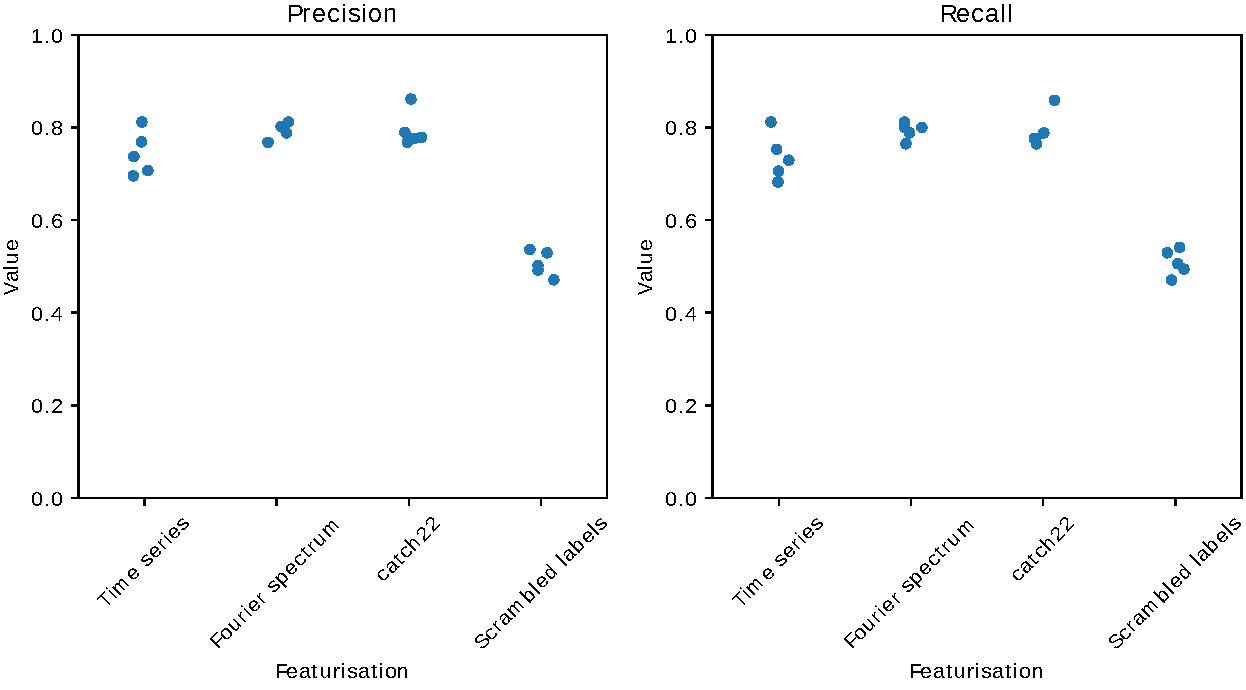
\includegraphics[width=0.9\textwidth]{svm_feat_compare_edit.pdf}
  \caption[
    Precision and recall from five-fold cross-validation of support vector classifiers trained using different featurisation methods.
  ]{
    (Left) Precision and (right) recall from five-fold cross-validation of support vector classifiers trained using different featurisation methods:
    using the time points as features,
    using the power values in the Fourier spectrum as features,
    and using \emph{catch22} features.
    As a control, the oscillatory and non-oscillatory labels were randomly reassigned to the time series and the time points were used as features.
  }
  \label{fig:analysis-precision-recall}
\end{figure}

% \begin{figure}
%   \centering
%   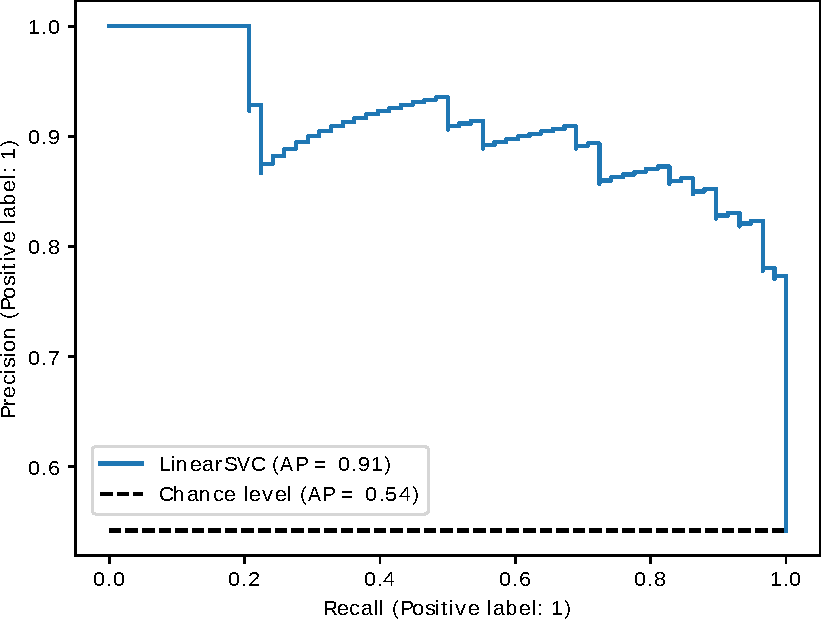
\includegraphics[width=0.7\textwidth]{svm_1_edit.pdf}
%   \caption[
%     Precision-recall curve of binary classifier
%   ]{
%     Precision-recall curve of binary classifier, using \textit{catch22} for featurisation and with a support vector classifier architecture (radial bias kernel, $\gamma = 1/22$, $C = 1$).
%   }
%   \label{fig:analysis-svc-pr}
% \end{figure}

To predict the probability that each time series was oscillatory, I used Platt scaling  \parencite{plattProbabilisticOutputsSupport1999} with the support vector classifier, as implemented by the \texttt{predict\_proba} method in the Python package \texttt{scikit\_learn}.
Platt scaling involves finding parameters for a logistic sigmoid function which approximates the posterior class probability for a binary classifier.
Fig.\ \ref{fig:analysis-svc-proba-histogram} suggests that the classifier performed well in discriminating between the two classes, as evidenced by the U-shaped histogram of probabilities (Fig.\ \ref{fig:analysis-svc-proba-histogram-model}), in contrast to the control (Fig.\ \ref{fig:analysis-svc-proba-histogram-scramble}).

\begin{figure}[ht!]
  \centering
  \begin{subfigure}[htpb]{0.45\textwidth}
   \centering
   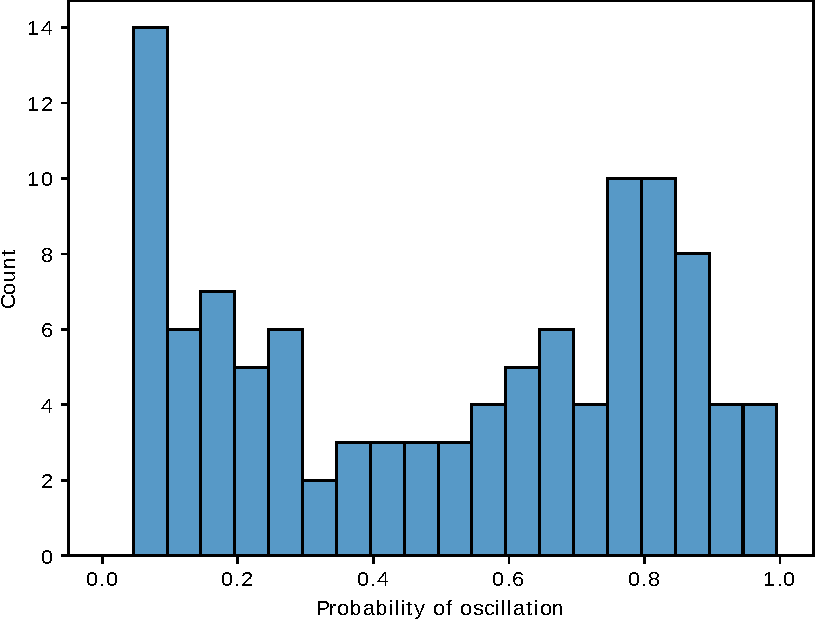
\includegraphics[width=\textwidth]{svm_2_edit.pdf}
   \caption{
   }
   \label{fig:analysis-svc-proba-histogram-model}
  \end{subfigure}%
  \begin{subfigure}[htpb]{0.45\textwidth}
   \centering
   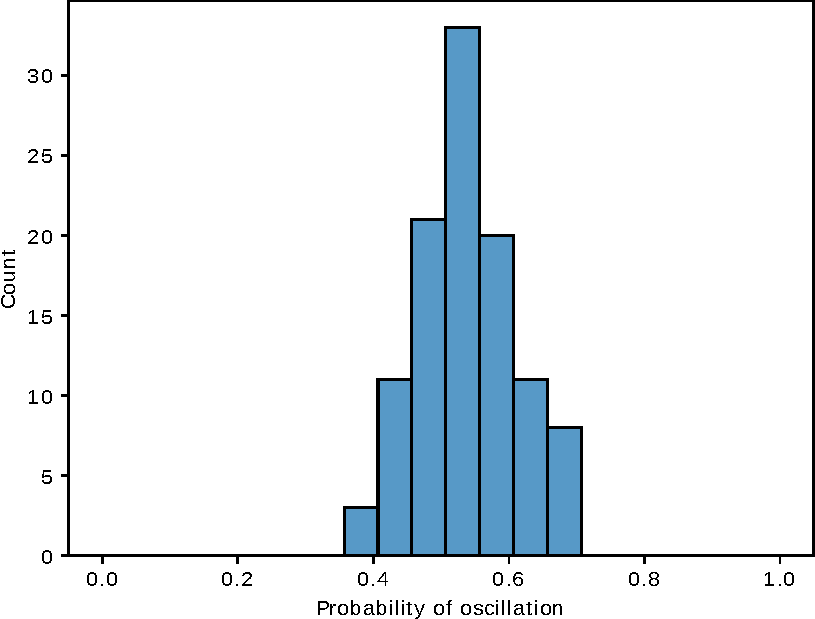
\includegraphics[width=\textwidth]{svm_scramble_2_edit.pdf}
   \caption{
   }
   \label{fig:analysis-svc-proba-histogram-scramble}
  \end{subfigure}

  \caption[
    Histogram of probabilities of whether a time series in the test data set is classified as oscillatory by the SVC, and as a control,
    with labels randomly re-assorted to time series.
  ]{
    \textbf{(\ref{fig:analysis-svc-proba-histogram-model})}
    Histogram of probabilities of whether a time series in the test data set is classified as oscillatory by the SVC (featurisation with \textit{catch22}, $\gamma = 1/22$, $C = 10$), and as a control
    \textbf{(\ref{fig:analysis-svc-proba-histogram-scramble})}
    with labels randomly reassigned.
  }
  \label{fig:analysis-svc-proba-histogram}
\end{figure}

In addition, Fig.\ \ref{fig:analysis-svc-proba-gallery} demonstrates that the probabilities can serve as a good score to rank time series by oscillation quality.

\begin{figure}[hb!]
  \centering
  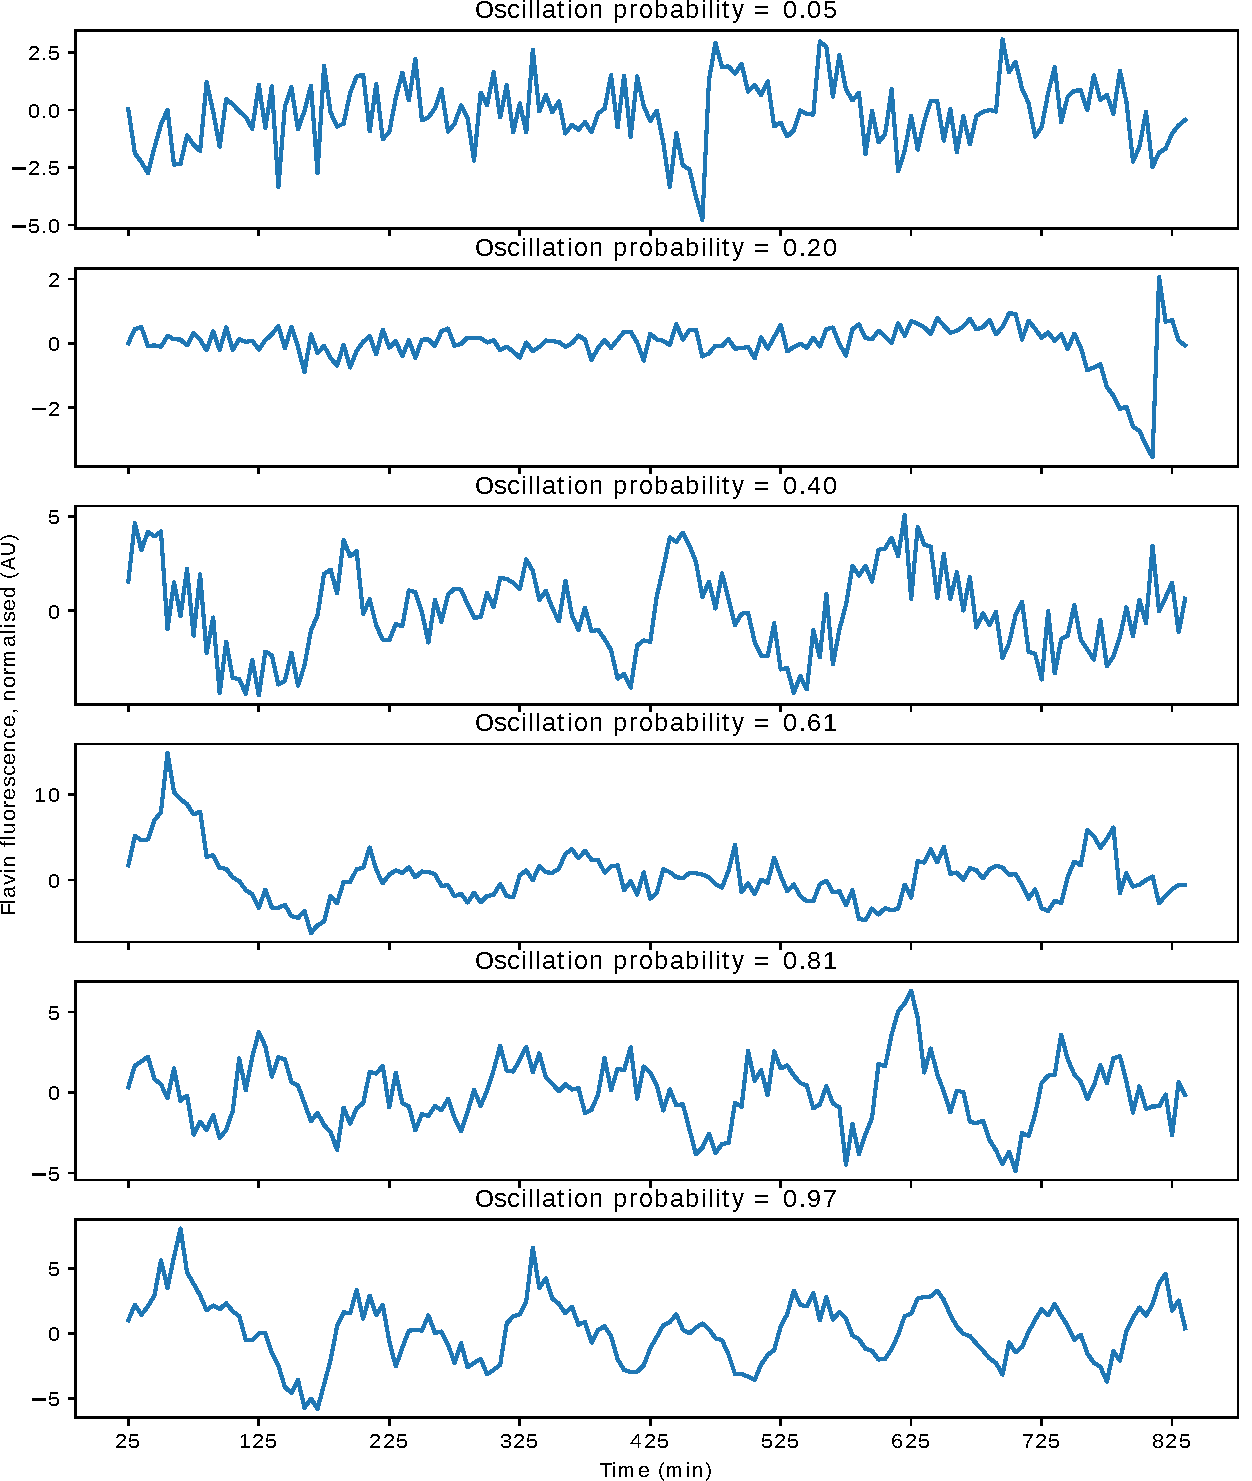
\includegraphics[width=0.65\textwidth]{svm_3_edit.pdf}

  \caption{
    Sample time series arranged by probability that each is oscillatory, as predicted by the support vector classifier.
  }
  \label{fig:analysis-svc-proba-gallery}
\end{figure}


\section{Period estimation using the autocorrelation function}
\label{sec:analysis-characterisation}

Estimating the period of oscillatory time series is important as it provides a quantitative measure of how yeast metabolic cycles respond to genetic nutrient perturbations as was previously used by \parencite{papagiannakisAutonomousMetabolicOscillations2017}.
To show that the autocorrelation function can be used to estimate the period and noise properties of both symmetric and asymmetric oscillations, I adapted the autocorrelation function as used by \textcite{pietschDeterminingGrowthRates2023} (Methods Section~\ref{subsec:methods-computational-xcf}).
To calibrate the method, I generated synthetic oscillations --- sinusoids and the FitzHugh-Nagumo oscillator \parencite{fitzhughImpulsesPhysiologicalStates1961} --- to investigate the effect of their properties on the autocorrelation function.
Subsequently, I applied the autocorrelation function to characterise experimentally-recorded time series.
Details on how the sinusoids and the FitzHugh-Nagumo oscillators were defined can be found in Methods Section~\ref{subsec:methods-computational-synthetic}.

\subsection{Effect of noise parameters on the autocorrelation function of synthetic sinusoids}
\label{subsec:analysis-characterisation-acf-sinusoid}

To compare the effect of Gaussian noise and Gillespie noise on the autocorrelation function, I computed the autocorrelation functions from a population of sinusoids with either type of noise added via element-wise sums.
% [Show working -- i.e. the mathematical derivations that make me expect results?]
% [Equations -- clear lines before/after, rather than having them in-line?]
Fig.\ \ref{fig:acf-sinusoids-nonoise-acf} shows that the autocorrelation function computed from a population of out-of-phase sinusoids could be modelled by a cosine with the same period as the sinusoids.
Following this, Fig.\ \ref{fig:acf-sinusoids-gausnoise-acf} shows that the addition of Gaussian noise preserved the point $(0,1)$, but the amplitude of the cosine that models the autocorrelation function was decreased.
Furthermore, the variation of the autocorrelation function among time series at long lags was increased, as evidenced by the interquartile range, because less data was used to compute the autocorrelation function at longer lags.% (mathematical derivation in appendix ...).

\begin{figure}
  \centering
  \begin{subfigure}[t]{0.6\textwidth}
  \centering
    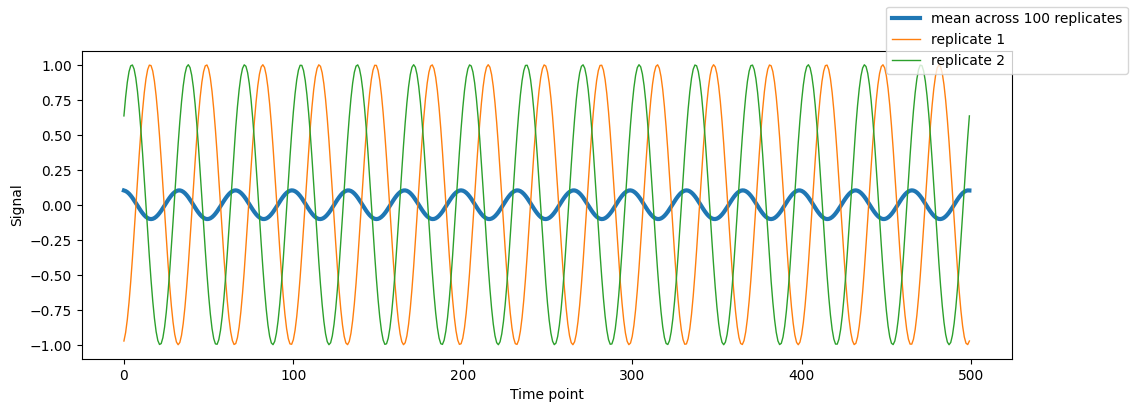
\includegraphics[width=\linewidth]{sinusoids_outofphase}
    \caption{
    }
    \label{fig:acf-sinusoids-nonoise-ts}
  \end{subfigure}%
  \centering
  \begin{subfigure}[t]{0.4\textwidth}
  \centering
    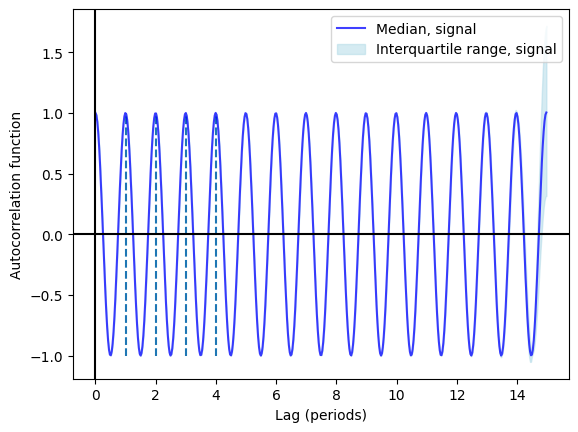
\includegraphics[width=\linewidth]{sinusoids_outofphase_acf_corrected}
    \caption{
    }
    \label{fig:acf-sinusoids-nonoise-acf}
  \end{subfigure}

  \begin{subfigure}[t]{0.6\textwidth}
  \centering
    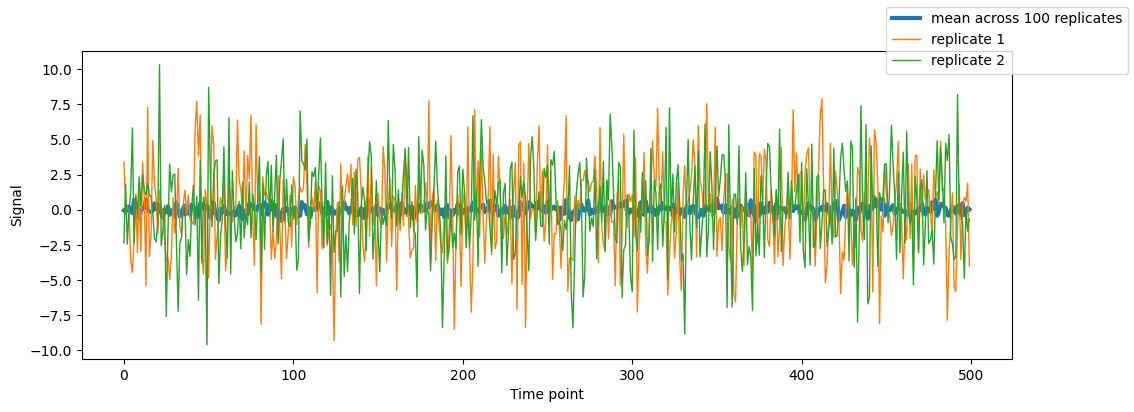
\includegraphics[width=\linewidth]{verynoisysinusoids_outofphase}
    \caption{
    }
    \label{fig:acf-sinusoids-gausnoise-ts}
  \end{subfigure}%
  \centering
  \begin{subfigure}[t]{0.4\textwidth}
  \centering
    \includegraphics[width=\linewidth]{verynoisysinusoids_outofphase_acf}
    \caption{
    }
    \label{fig:acf-sinusoids-gausnoise-acf}
  \end{subfigure}

  \begin{subfigure}[t]{0.6\textwidth}
  \centering
    \includegraphics[width=\linewidth]{gillespie_k5_d0p05_mean}
    \caption{
    }
    \label{fig:acf-sinusoids-gillnoise-ts}
  \end{subfigure}%
  \centering
  \begin{subfigure}[t]{0.4\textwidth}
  \centering
    \includegraphics[width=\linewidth]{gillespie_k5_d0p05_acf}
    \caption{
    }
    \label{fig:acf-sinusoids-gillnoise-acf}
  \end{subfigure}

  \caption[
    Sample sinusoids without noise, with Gaussian noise, and with Gillespie noise, along with their autocorrelation functions.
  ]{
    %Effect of type of noise on the autocorrelation function.
    \textbf{(\ref{fig:acf-sinusoids-nonoise-ts})} Sample sinusoids without noise, and
    \textbf{(\ref{fig:acf-sinusoids-nonoise-acf})} its autocorrelation function.
    %
    \textbf{(\ref{fig:acf-sinusoids-gausnoise-ts})} Sample sinusoids with Gaussian noise defined by drawing samples from $\mathcal{N}(0,\sigma^{2}=3)$, and
    \textbf{(\ref{fig:acf-sinusoids-gausnoise-acf})} its autocorrelation function.
    %
    \textbf{(\ref{fig:acf-sinusoids-gillnoise-ts})} Sample sinusoids of with Gillespie noise ($k_{0} = 5$ and $d_{0} = 0.05$), and
    \textbf{(\ref{fig:acf-sinusoids-gillnoise-acf})} its autocorrelation function.
    Red line is defined by $y = \me^{-2d_{0}T}$, where $T$ represents the lag in units of period of the sinusoids.
    %
    For each case, the frequency of the sinusoids was 0.03, and there were 100 repeats, randomly out-of-phase.
  }
  \label{fig:acf-sinusoids}
\end{figure}

Gillespie noise is based on the birth-death process (Fig.\ \ref{fig:analysis-birthdeath-process}), and its two parameters control noise parameters (Methods Section~\ref{subsec:methods-computational-synthetic}).
Specifically, given a birth rate $k_{0}$ and a death rate $d_{0}$, the noise has a standard deviation of noise amplitude $A = \sqrt{k_{0}/d_{0}}$ and noise timescale $\tau = 1/d_{0}$.

\begin{figure}[p]
  \centering
  \begin{subfigure}[t]{0.6\textwidth}
    \centering
    \includegraphics[width=\textwidth]{birth_death_process}
    \caption{
    }
    \label{fig:analysis-birthdeath-process-illustration}
  \end{subfigure}

  \begin{subfigure}[t]{0.4\textwidth}
    \centering
    \includegraphics[width=\textwidth]{gillespie}
    \caption{
    }
    \label{fig:gillespie_trajectory}
  \end{subfigure}

  \caption[
    Illustration of the birth-death process.
  ]{
    \textbf{(\ref{fig:analysis-birthdeath-process-illustration})}
    Illustration of the birth-death process.
    The birth-death process is defined by two reactions: birth ($R_{1}: \varnothing \ce{ -> P}$), with rate $k_{0}$, and death ($R_{2}: \ce{P -> } \varnothing$) with rate $d_{0}$, both of which affect the number $N$ of species $P$.
    Random firing of the birth and death reactions, simulated by the Gillespie algorithm \parencite{gillespieStochasticSimulationChemical2007}, defines the trajectory of $N$ over time, which in turn defines Gillespie noise.
    \textbf{(\ref{fig:gillespie_trajectory})}
    Sample trajectory of a substrate created and destroyed by the birth-death process, simulated by the Gillespie algorithm ($k_{0} = 5$, $d_{0} = 0.05$, $t_{\mathrm{max}} = 1500$).
  }
  \label{fig:analysis-birthdeath-process}
\end{figure}

% [Show working -- i.e. the mathematical derivations that make me expect this exponential fit?]
% Though Peter said this `is not trivial'.
Fig.\ \ref{fig:acf-sinusoids-gillnoise-acf} shows that when Gillespie noise was added to the sinusoids, the medium autocorrelation followed the exponential decay function $y = \me^{-2d_{0}T}$, where $T$ represents lag.
In addition, the locations of the peaks of the autocorrelation function were preserved.
The observation thus suggests that the death rate $d_{0}$ parameter of Gillespie noise controlled the shape of the autocorrelation function.

% \begin{figure}
%   \centering
%   \begin{subfigure}[t]{0.5\textwidth}
%   \centering
%     \includegraphics[width=\linewidth]{acf_fit_example.png}
%     \caption{
%     }
%     \label{fig:acf-noisetimescale-effect-fit}
%   \end{subfigure}%
%   \begin{subfigure}[t]{0.5\textwidth}
%   \centering
%     \includegraphics[width=\linewidth]{deathrate_vs_decay.png}
%     \caption{
%     }
%     \label{fig:acf-noisetimescale-effect-relationship}
%   \end{subfigure}

%   \caption[
%     Fitting exponential decay functions to estimate $d_{0}$ from the autocorrelation function.
%   ]{
%     \textbf{(\ref{fig:acf-noisetimescale-effect-fit})} Fitting exponential decay functions to estimate $d_{0}$ from the autocorrelation function.
%     \textbf{(\ref{fig:acf-noisetimescale-effect-relationship})} The relationship between $d_{0}$ and the decay rate $D$ found from fitting exponential decay functions to the mean autocorrelation function, the peaks, and the troughs of this mean function.
%     Here, $k_{0}$ was held constant at 5.
%   }
%   \label{fig:acf-noisetimescale-effect}
% \end{figure}

To quantify the effect of the noise timescale on the shape of the autocorrelation function, I varied the death rate parameter $d_{0}$ when generating Gillespie noise.
Fig.\ \ref{fig:acf-noisetimescale} shows that a higher death rate decreased the decay timescale of the autocorrelation function (Fig.\ \ref{fig:acf-noisetimescale-highd0-acf}), while a lower death rate introduced long-term trends in the simulated signals (Fig.\ \ref{fig:acf-noisetimescale-lowd0-ts}).
A lower death rate also increased the variation between autocorrelation functions between replicates (Fig.\ \ref{fig:acf-noisetimescale-lowd0-acf}).

\begin{figure}
  \centering
  \begin{subfigure}[t]{0.6\textwidth}
  \centering
    \includegraphics[width=\linewidth]{gillespie_k5_d0p5_mean.png}
    \caption{
    }
    \label{fig:acf-noisetimescale-highd0-ts}
  \end{subfigure}%
  \begin{subfigure}[t]{0.4\textwidth}
  \centering
    \includegraphics[width=\linewidth]{gillespie_k5_d0p5_acf.png}
    \caption{
    }
    \label{fig:acf-noisetimescale-highd0-acf}
  \end{subfigure}

  \begin{subfigure}[t]{0.6\textwidth}
  \centering
    \includegraphics[width=\linewidth]{gillespie_k5_d0p005_mean.png}
    \caption{
    }
    \label{fig:acf-noisetimescale-lowd0-ts}
  \end{subfigure}%
  \begin{subfigure}[t]{0.4\textwidth}
  \centering
    \includegraphics[width=\linewidth]{gillespie_k5_d0p005_acf.png}
    \caption{
    }
    \label{fig:acf-noisetimescale-lowd0-acf}
  \end{subfigure}

  \caption[
    Effect of death rate of Gillespie noise on the autocorrelation function.
  ]{
    %Effect of death rate ($d_{0}$) of Gillespie noise on the autocorrelation function.
    \textbf{(\ref{fig:acf-noisetimescale-highd0-ts})} Sample sinusoids with Gillespie noise ($k_{0} = 5$ and $d_{0} = 0.5$), and
    \textbf{(\ref{fig:acf-noisetimescale-highd0-acf})} its autocorrelation function.
    %
    \textbf{(\ref{fig:acf-noisetimescale-lowd0-ts})} Sample sinusoids with Gillespie noise ($k_{0} = 5$ and $d_{0} = 0.005$), and
    \textbf{(\ref{fig:acf-noisetimescale-lowd0-acf})} its autocorrelation function.
    %
    Red lines are defined by $y = \me^{-2d_{0}T}$, where $T$ represents the lag in units of period of the sinusoids.
    %
    For each case, the frequency of the sinusoids was 0.03, and there were 100 repeats, randomly out-of-phase.
  }
  \label{fig:acf-noisetimescale}
\end{figure}

% To show how $d_{0}$ can be estimated from the autocorrelation function, I fitted exponential decay functions to the mean autocorrelation, the peaks of the mean function, and the troughs of the mean functions using non-linear least squares fitting (Fig.\ \ref{fig:acf-noisetimescale-effect-fit}).
% The functions were of the form:

% \begin{equation}
%   y = (1-C)\me^{-DT}+C
%   \label{eq:acf-expofit}
% \end{equation}

% where $y$ represents the vertical axis (autocorrelation axis), $T$ represents the lag multiples of the period of the sinusoid oscillator, and with $C$ and $D$ being variable parameters whose values are to be determined.

% Fig.\ \ref{fig:acf-noisetimescale-effect-relationship} suggests that the decay rates $D$ of the autocorrelation function increases linearly with $d_{0}$.
% In other words, the death rate $d_{0}$ controls the decay rate $D$ of the autocorrelation function.
% Conversely, if $D$ can be estimated from the autocorrelation function, then the noise timescale of the time series can be estimated.


% \begin{figure}
%   \centering
%   \includegraphics[width=0.6\linewidth]{birthrate_vs_ydispl.png}
%   \caption[
%     The relationship between the noise amplitude and the $y$-displacement $C$ found from fitting exponential decay functions to the mean autocorrelation function.
%   ]{
%     The relationship between the noise amplitude and the $y$-displacement $C$ found from fitting exponential decay functions to the mean autocorrelation function, the peaks, and the troughs of this mean function.
%     Here, $d_{0}$ was held constant at 0.05.
%   }
%   \label{fig:acf-noiseamplitude-effect}
% \end{figure}

To quantify the effect of the noise amplitude on the autocorrelation function, I varied the birth rate parameter $k_{0}$ when generating Gillespie noise.
Fig.\ \ref{fig:acf-noiseamplitude} shows that a higher birth rate increased the amplitude of noise (Fig.\ \ref{fig:acf-noiseamplitude-highk0-ts}) and increased the variation between replicate autocorrelation functions (Fig.\ \ref{fig:acf-noiseamplitude-highk0-acf}), while the opposite was true for a higher birth rate (Figs.\ \ref{fig:acf-noiseamplitude-lowk0-ts}--\ref{fig:acf-noiseamplitude-lowk0-acf}).

\begin{figure}
  \centering
  \begin{subfigure}[t]{0.6\textwidth}
  \centering
    \includegraphics[width=\linewidth]{gillespie_k25_d0p05_mean.png}
    \caption{
    }
    \label{fig:acf-noiseamplitude-highk0-ts}
  \end{subfigure}%
  \begin{subfigure}[t]{0.4\textwidth}
  \centering
    \includegraphics[width=\linewidth]{gillespie_k25_d0p05_acf.png}
    \caption{
    }
    \label{fig:acf-noiseamplitude-highk0-acf}
  \end{subfigure}

  \begin{subfigure}[t]{0.6\textwidth}
  \centering
    \includegraphics[width=\linewidth]{gillespie_k1_d0p05_mean.png}
    \caption{
    }
    \label{fig:acf-noiseamplitude-lowk0-ts}
  \end{subfigure}%
  \begin{subfigure}[t]{0.4\textwidth}
  \centering
    \includegraphics[width=\linewidth]{gillespie_k1_d0p05_acf.png}
    \caption{
    }
    \label{fig:acf-noiseamplitude-lowk0-acf}
  \end{subfigure}

  \caption[
    Effect of birth rate of Gillespie noise on the autocorrelation function.
  ]{
    %Effect of birth rate ($k_{0}$) of Gillespie noise on the autocorrelation function.
    \textbf{(\ref{fig:acf-noiseamplitude-highk0-ts})} Sample sinusoids with Gillespie noise ($k_{0} = 25$ and $d_{0} = 0.05$), and
    \textbf{(\ref{fig:acf-noiseamplitude-highk0-acf})} its autocorrelation function.
    %
    \textbf{(\ref{fig:acf-noiseamplitude-lowk0-ts})} Sample sinusoids with Gillespie noise ($k_{0} = 1$ and $d_{0} = 0.05$), and
    \textbf{(\ref{fig:acf-noiseamplitude-lowk0-acf})} its autocorrelation function.
    %
    Red lines are defined by $y = \me^{-2d_{0}T}$, where $T$ represents the lag in units of period of the sinusoids.
    %
    For each case, the frequency of the sinusoids was 0.03, and there were 100 repeats, randomly out-of-phase.
  }
  \label{fig:acf-noiseamplitude}
\end{figure}

% To show how the noise amplitude can be estimated from the autocorrelation function, I fit exponential decay functions (Eq.\ \ref{eq:acf-expofit}) as in Fig.\ \ref{fig:acf-noisetimescale-effect-fit}.
% Fig.\ \ref{fig:acf-noiseamplitude-effect} suggests that the $y$-displacements $C$ of the exponential fits to peaks and troughs converged to 0 as $k_{0}/d_{0}$ increased, showing that the amplitude of the oscillations in the autocorrelation function decreases as the noise amplitude increases.
% In other words, the birth rate $d_{0}$ controls the $y$-displacement parameter $C$ of the autocorrelation function, which is a proxy for the function's amplitude.
% Conversely, if $C$ can be estimated from the autocorrelation function, then the noise amplitude of the time series can be estimated.


\subsection{FitzHugh-Nagumo oscillator: effect of oscillation shape}
\label{subsec:analysis-characterisation-acf-fhn}

% \begin{figure}
%   \centering
%   \begin{subfigure}[t]{0.45\textwidth}
%   \centering
%     \includegraphics[width=\linewidth]{fhn_expofit}
%     \caption{
%     }
%     \label{fig:acf-fhn-noiseparams-fit}
%   \end{subfigure}%
%   \begin{subfigure}[t]{0.45\textwidth}
%   \centering
%     \includegraphics[width=\linewidth]{fhn_highnts_expofit}
%     \caption{
%     }
%     \label{fig:acf-fhn-noiseparams-fit-highnts}
%   \end{subfigure}
%
%   \begin{subfigure}[t]{0.45\textwidth}
%   \centering
%     \includegraphics[width=\linewidth]{fhn_deathrate_vs_decay.png}
%     \caption{
%     }
%     \label{fig:acf-fhn-noiseparams-noisetimescale}
%   \end{subfigure}%
%   \begin{subfigure}[t]{0.45\textwidth}
%   \centering
%     \includegraphics[width=\linewidth]{fhn_birthrate_vs_ydispl.png}
%     \caption{
%     }
%     \label{fig:acf-fhn-noiseparams-noiseamplitude}
%   \end{subfigure}

%   \caption[
%     Effect of Gillespie noise parameters on the autocorrelation function of FitzHugh-Nagumo oscillators.
%   ]{
%     \textbf{(\ref{fig:acf-fhn-noiseparams-fit})}
%     Fitting exponential decay functions of the form $y = (1-C)\me^{-DT}+C$, with $C$ and $D$ as variable parameters, to the autocorrelation function, generated with $k_{0}=5$ and $d_{0}=0.05$, and
%     \textbf{(\ref{fig:acf-fhn-noiseparams-fit-highnts})}
%     with $k_{0}=5$ and $d_{0}=0.005$.
%     \textbf{(\ref{fig:acf-fhn-noiseparams-noisetimescale})}
%     The relationship between $d_{0}$ and the decay rate $D$ ($k_{0}=5$).
%     \textbf{(\ref{fig:acf-fhn-noiseparams-noiseamplitude})}
%     The relationship between $k_{0}/d_{0}$ and $y$-displacement $C$ of the exponential fit ($d_{0}=0.05$)
%   }
%   \label{fig:acf-fhn-noiseparams}
% \end{figure}

To test whether Gillespie noise parameters can be estimated from the autocorrelation function computed from an asymmetric oscillation, I added Gillespie noise with varying $d_{0}$ and $k_{0}$ to FitzHugh-Nagumo oscillators as defined in the Methods Section~\ref{subsec:methods-computational-synthetic}.
%I repeated the exponential fitting in section~\ref{subsec:analysis-characterisation-acf-sinusoid} on the FitzHugh-Nagumo oscillator as defined in the Methods (Section~\ref{subsec:methods-computational-synthetic}).
Fig.\ \ref{fig:acf-fhn-gillnoise-acf} shows that when the oscillator had a different shape, the waves in the autocorrelation function changed shape, becoming more pointed.
Additionally, the effect of noise parameters on the autocorrelation function is preserved when the oscillators switch from sinusoid to FitzHugh-Nagumo oscillators.
% In addition, Fig.\ \ref{fig:acf-fhn-noiseparams-fit-highnts} suggests that fitting an exponential decay function to the autocorrelation function to estimate noise parameters was less reliable, particularly with high noise timescales.
% As a consequence, estimating the noise timescale $\tau$ from the decay rate $D$ of the exponential decay function produced a greater range of uncertainty (Fig.\ \ref{fig:acf-fhn-noiseparams-noisetimescale}).
% However, estimating the noise amplitude $A$ based on the y-displacement $C$ of the exponential decay function remained as reliable as the sinusoid oscillator case (Fig.\ \ref{fig:acf-fhn-noiseparams-noiseamplitude}).

\begin{figure}[hb!]
  \centering
  \begin{subfigure}[t]{0.6\textwidth}
  \centering
    \includegraphics[width=\linewidth]{fhn_meanplot}
    \caption{
    }
    \label{fig:acf-fhn-gillnoise-ts}
  \end{subfigure}%
  \begin{subfigure}[t]{0.4\textwidth}
  \centering
    \includegraphics[width=\linewidth]{fhn_acf}
    \caption{
    }
    \label{fig:acf-fhn-gillnoise-acf}
  \end{subfigure}

  \caption[
    Sample FitzHugh-Nagumo oscillators with Gillespie noise, and
    its autocorrelation function.
  ]{
    %The autocorrelation function of FitzHugh-Nagumo oscillators with Gillespie noise.
    \textbf{(\ref{fig:acf-fhn-gillnoise-ts})} Sample FitzHugh-Nagumo oscillators ($RI_{\mathrm{ext}}$ = 0.4, $\tau$ = 12.5, $a$ = 0.7, $b$ = 0.82) with Gillespie noise ($k_{0} = 5$ and $d_{0} = 0.05$), and
    \textbf{(\ref{fig:acf-fhn-gillnoise-acf})} its autocorrelation function.
    Red line is defined by $y = \me^{-2d_{0}T}$, where $T$ represents the lag in units of period of the sinusoids.
    %
    There were 100 repeats, randomly out-of-phase.
  }
  \label{fig:acf-fhn}
\end{figure}


\subsection{Real data from fluorescence microscopy in microfluidics experiments}
\label{subsubsec:analysis-characterisation-real}

To deduce the period and noise parameters of a experimentally-recorded sinusoid-like signal (Fig.\ \ref{fig:acf-sinusoid-biol-ts}), I computed the autocorrelation functions of a population of flavin autofluorescence time series (Fig.\ \ref{fig:acf-sinusoid-biol-acf}).
% , and fitted exponential functions to the mean autocorrelation function, scaled to have amplitudes and periods fit the simulated sinusoids (Fig.\ \ref{fig:acf-sinusoid-biol-acf-fit}).
The autocorrelation function suggests an average period of 19 time points, corresponding to \SI{95}{\minute}, as expected from the nutrient conditions.
However, estimation of noise parameters was complicated by the damping in the autocorrelation function, giving a different shape compared to the synthetic data and fewer peaks and troughs for fitting.
Nevertheless, relating the shape of the autocorrelation function to the effect of noise parameters on synthetic sinusoids suggested a noise timescale of 7.35 and a noise amplitude of 110.45.
% Nevertheless, the decay rate $D$ of the exponential function fitted to the mean autocorrelation function suggested a noise timescale of 7.35 and the y-displacement $C$ of the exponential function fitted to the peaks of the autocorrelation function suggested a noise amplitude of 161.84.

\begin{figure}
  \centering
  \begin{subfigure}[t]{0.6\textwidth}
  \centering
    \includegraphics[width=\linewidth]{acf_sinusoid_biol_ts.png}
    \caption{
    }
    \label{fig:acf-sinusoid-biol-ts}
  \end{subfigure}%
  \begin{subfigure}[t]{0.4\textwidth}
  \centering
    \includegraphics[width=\linewidth]{acf_sinusoid_biol_acf.png}
    \caption{
    }
    \label{fig:acf-sinusoid-biol-acf}
  \end{subfigure}

  % \begin{subfigure}[t]{0.5\textwidth}
  % \centering
  %   \includegraphics[width=\linewidth]{acf_sinusoid_biol_acf_fit.png}
  %   \caption{
  %   }
  %   \label{fig:acf-sinusoid-biol-acf-fit}
  % \end{subfigure}

  \caption[
    Sample time series of flavin autofluorescence, its autocorrelation function, and fitting exponential decay functions.
  ]{
    \textbf{(\ref{fig:acf-sinusoid-biol-ts})}
    Sample time series of flavin autofluorescence.
    \textbf{(\ref{fig:acf-sinusoid-biol-acf})}
    Autocorrelation function across a population of time series of flavin autofluorescence.
    % \textbf{(\ref{fig:acf-sinusoid-biol-acf-fit})}
    % Fitting exponential decay functions to determine noise parameters, lag axis scaled to match Fig.\ \ref{fig:acf-noisetimescale-effect}.
  }
  \label{fig:acf-sinusoid-biol}
\end{figure}

In addition to flavin autofluorescence, I also recorded time series of histone 2B abundance as an indicator of the phases of the cell division cycle \parencite{garmendia-torresMultipleInputsEnsure2018}, to investigate whether the flavin autofluorescence oscillations and the cell division cycle synchronised.
The abundance of histone 2B follow an asymmetric oscillation (Fig.\ \ref{fig:acf-fhn-biol-ts}).

\begin{figure}
  \centering
  \begin{subfigure}[t]{0.6\textwidth}
  \centering
    \includegraphics[width=\linewidth]{acf_fhn_biol_ts.png}
    \caption{
    }
    \label{fig:acf-fhn-biol-ts}
  \end{subfigure}%
  \begin{subfigure}[t]{0.4\textwidth}
  \centering
    \includegraphics[width=\linewidth]{acf_fhn_biol_acf.png}
    \caption{
    }
    \label{fig:acf-fhn-biol-acf}
  \end{subfigure}

  % \begin{subfigure}[t]{0.5\textwidth}
  % \centering
  %   \includegraphics[width=\linewidth]{acf_fhn_biol_acf_fit.png}
  %   \caption{
  %   }
  %   \label{fig:acf-fhn-biol-acf-fit}
  % \end{subfigure}

  \caption[
    Sample time series of histone 2B abundance, its autocorrelation function, and fitting exponential decay functions.
  ]{
    \textbf{(\ref{fig:acf-fhn-biol-ts})}
    Sample time series of histone 2B abundance.
    \textbf{(\ref{fig:acf-fhn-biol-acf})}
    Autocorrelation function across a population of time series of histone 2B abundance.
    % \textbf{(\ref{fig:acf-fhn-biol-acf-fit})}
    % Fitting exponential decay functions to determine noise parameters.
  }
  \label{fig:acf-fhn-biol}
\end{figure}

Similar to the previous section, to deduce the period and noise parameters of this signal, I computed the autocorrelation functions of a population of histone 2B abundance time series (Fig.\ \ref{fig:acf-fhn-biol-acf}).
% , and fitted exponential functions to the mean autocorrelation function, scaled to have amplitudes and periods fit the simulated FitzHugh-Nagumo oscillators (Fig.\ \ref{fig:acf-fhn-biol-acf-fit}).
The autocorrelation function also suggests an average period of 19 time points, corresponding to \SI{95}{\minute}.
As was the case for the flavin autofluorescence time series, the damping in the autocorrelation function complicated estimation of noise parameters, but the function suggested a noise timescale of 9.35 and a noise amplitude of 168.12.
%; though the decay rate $D$ of the exponential function fitted to the mean autocorrelation function suggested a noise timescale of 11.19 and the y-displacement $C$ of the exponential function fitted to the peaks of the autocorrelation function suggested a noise amplitude of 292.41.
The differences of these noise parameters relative to the flavin autofluorescence time series suggest different noise properties, which can be explained by the different fluorescence channels and exposure times used to generate each type of signal.


\section{Detection of synchrony}
\label{sec:analysis-correlation}

To test a method to detect the synchrony and quantify the temporal lag between two types of oscillations, I computed the cross-correlation functions of a population of sinusoid and FitzHugh-Nagumo oscillators.
Cross-correlation has been used to investigate the relationship between the expression levels of two genes in a model feed-forward loop \parencite{dunlopRegulatoryActivityRevealed2008},
and to investigate the relationship between instantaneous growth rate and the expression of \textit{lac} genes of enzymes in central metabolism across a population of \textit{E. coli} cells \parencite{kivietStochasticityMetabolismGrowth2014}.


\subsection{Synthetic data}
\label{subsubsec:analysis-correlation-synthetic}

Fig.\ \ref{fig:xcf-nonoise-xcf} shows that the cross-correlation function identifies that the sinusoids, on average, peaked 20 time points before the FitzHugh-Nagumo oscillators, close to the actual value of 20.75 time points.
This shift was evidenced by the position of the peak of the cross-correlation function closest to the vertical axis.
The cross-correlation function further showed that synchrony between the two oscillators was maintained along the entire time series, across all time series.
Furthermore, Fig.\ \ref{fig:xcf-gillnoise-xcf} suggests that even with strong Gillespie noise, the lag between the two oscillators could still be deduced from the cross-correlation function.

\begin{figure}[hb!]
  \centering
  \begin{subfigure}[t]{0.6\textwidth}
  \centering
    \includegraphics[width=\linewidth]{sinusoid_and_fitzhughnagumo_nonoise.png}
    \caption{
    }
    \label{fig:xcf-nonoise-ts}
  \end{subfigure}%
  \centering
  \begin{subfigure}[t]{0.4\textwidth}
  \centering
    \includegraphics[width=\linewidth]{randomshift_sinusoid_fitzhughnagumo_xcf.png}
    \caption{
    }
    \label{fig:xcf-nonoise-xcf}
  \end{subfigure}

  \begin{subfigure}[t]{0.6\textwidth}
  \centering
    \includegraphics[width=\linewidth]{sinusoid_and_fitzhughnagumo_gillnoise.png}
    \caption{
    }
    \label{fig:xcf-gillnoise-ts}
  \end{subfigure}%
  \centering
  \begin{subfigure}[t]{0.4\textwidth}
  \centering
    \includegraphics[width=\linewidth]{randomshift_sinusoid_fitzhughnagumo_gillnoise_xcf.png}
    \caption{
    }
    \label{fig:xcf-gillnoise-xcf}
  \end{subfigure}

  \caption[
    Sample sinusoid and FitzHugh-Nagumo oscillators without noise and with Gillespie noise, along with their cross-correlation functions.
  ]{
    %Using the cross-correlation function to evaluate the shift of one synthetic time series relative to another with a different shape.
    \textbf{(\ref{fig:xcf-nonoise-ts})}
    (Blue) Sample sinusoid ($f = 0.0235$) and (orange) FitzHugh-Nagumo oscillator ($RI_{\mathrm{ext}}$ = 0.4, $\tau$ = 12.5, $a$ = 0.7, $b$ = 0.82) of the same frequency and without noise, and
    \textbf{(\ref{fig:xcf-nonoise-xcf})}
    the cross-correlation function of the FitzHugh-Nagumo oscillators with respect to the sinusoids.
    %
    \textbf{(\ref{fig:xcf-gillnoise-ts})}
    (Blue) Sample sinusoid and (orange) FitzHugh-Nagumo oscillator with same parameters as \ref{fig:xcf-nonoise-ts}, but with Gillespie noise ($d_{0} = 0.05$, $k_{0} = 5$), and
    \textbf{(\ref{fig:xcf-gillnoise-xcf})}
    the cross-correlation function of the FitzHugh-Nagumo oscillators with respect to the sinusoids.
    %
    For each case, there were 400 repeats, randomly out-of-phase.
  }
  \label{fig:xcf}
\end{figure}


\subsection{Real data from fluorescence microscopy in microfluidics experiments}
\label{subsubsec:analysis-correlation-real}

To show how the cross-correlation function can be used to quantify the synchrony between flavin autofluorescence oscillations and HTB2::mCherry levels in a population of cells, Fig.\ \ref{fig:xcf-biol} displays a sample pair of time series (Fig.\ \ref{fig:xcf-biol-ts}) and the cross-correlation function from the population of cells (Fig.\ \ref{fig:xcf-biol-xcf}).
The cross-correlation function suggests that the histone 2B oscillations peaked after the flavin autofluorescence oscillations by an average of \SI{5}{\minute}.

\begin{figure}
  \centering
  \begin{subfigure}[t]{1.0\textwidth}
  \centering
    \includegraphics[width=\linewidth]{single_birth_plot_nostar.pdf}
    \caption{
    }
    \label{fig:xcf-biol-ts}
  \end{subfigure}

  \begin{subfigure}[t]{0.7\textwidth}
  \centering
    \includegraphics[width=\linewidth]{xcf_edit.pdf}
    \caption{
    }
    \label{fig:xcf-biol-xcf}
  \end{subfigure}

  \caption[
    Sample time series of flavin autofluorescence and histone 2B abundance, along with the cross-correlation function.
  ]{
    \textbf{(\ref{fig:xcf-biol-ts})}
    Sample time series of flavin autofluorescence (blue) and histone 2B abundance (orange).
    \textbf{(\ref{fig:xcf-biol-xcf})}
    Cross-correlation function between the flavin autofluorescence time series and the histone 2B abundance time series.
  }
  \label{fig:xcf-biol}
\end{figure}


\section{Discussion}
\label{sec:analysis-discussion}

This chapter discusses methods to filter long-term trends in time series data, to visualise structures within a dataset of time series, to detect rhythmicity in a time series, to estimate period and noise parameters, and to detect the synchrony between two time series.

My results suggest that using a high-pass Butterworth filter to filter out long-term trends in time series data gives better control over the frequency profile of the time series than moving-average methods, which is often used to detrend time series from biological oscillators.
Such results highlight that a degree of caution is needed to choose methods for such a crucial step in data analysis.

My exploration of UMAP and modularity clustering suggests that both methods were useful in discovering structure within time series, particularly in discriminating between oscillatory and non-oscillatory time series.
These methods further indicated sub-groups of time series that may have similar properties, such as shape or oscillation quality, which may correspond to sub-populations of metabolic cycle-producing cells in a culture.
The consistency between the two methods strongly suggest that such groups in the dataset are meaningful.

Subsequently, my exploration of three approaches to detect rhythmicity --- deriving a statistical test of a power spectrum, deriving a periodogram from an autoregressive model, and a binary classifier --- highlights the difficulty of rhythmicity detection in noisy biological time series.
The spectral method described by \textcite{glynnDetectingPeriodicPatterns2006} had a modest performance.
The autoregressive model was able to identify the most likely period in some time series, but otherwise classified most time series as non-oscillatory, and lacked a tuning parameter.
Finally, the support vector classifier suggests that a simple machine learning model could be adapted for rhythmicity detection, subject to a good feature set and training data.

Ultimately, rhythmicity detection requires supplying a threshold in some form, be it a range of frequencies in which oscillations are expected \parencite{zielinskiStrengthsLimitationsPeriod2014}, a parameter that controls the proportion of time series detected as oscillatory, or training labels.
This is because there is no way to objectively specify a failure rate for a rhythmicity detection method as there is no independent method to estimate rhythmicity \parencite{zielinskiStrengthsLimitationsPeriod2014}.

My observations concerning the autocorrelation function confirms its use for estimating the period of an oscillatory time series, as used previously by \textcite{papagiannakisAutonomousMetabolicOscillations2017}.
As periodicity-estimation methods have a limited ability to estimate the period of short, noisy time series owing to little input data, combining several such methods can be useful to produce a picture of the periodicity of oscillatory time series.
For example, \textcite{potvin-trottierSynchronousLongtermOscillations2016} combines the autocorrelation function and the Fourier transform to study the changes in the periodicity of a modified model of the repressilator.

Furthermore, I showed that the autocorrelation function may be used to estimate parameters to describe noise, assuming that the noise can be modelled by the birth-death process.
However, further work, such as synthetic time series generated from a wider variety of parameters or additional estimation methods are likely required for adequate estimation of noise parameters from real data.
In addition, it is possible that other types of noise better describe the noise from real data, and such types of noise may lead to different effects on the autocorrelation function.

Finally, my results show that the cross-correlation function, as used by \textcite{dunlopRegulatoryActivityRevealed2008}, \textcite{kivietStochasticityMetabolismGrowth2014}, and \textcite{pietschDeterminingGrowthRates2023}, can be used to detect synchrony between two sets of time series and to quantify the temporal relationship between the time series, even if the time series are very noisy.

Taken together, the analysis methods discussed in this chapter can form the basis of a powerful data analysis pipeline to analyse large datasets of oscillatory biological time series.

% \chapter{Microfluidics and fluorescence microscopy for cellular metabolic cycles}
\label{ch:biology}

To reconcile the evidence about the characteristics of the YMC from single-cell and chemostat experiments, I sought to use a single-cell experimental platform to address whether cellular metabolic cycles confirm chemostat-based studies.

There is a paucity of studies of the yeast metabolic cycle at the cellular level --- i.e.\ in which budding yeast cells are investigated in isolation rather than as a population.
Previous population-level studies in the chemostat, by their very nature, fail to account for cell-to-cell heterogeneity and create cell density and environmental conditions that are far removed from the natural habitat of budding yeast.

Here, I use single-cell microfluidics to physically separate budding yeast cells and use fluorescence microscopy to monitor the yeast metabolic cycle and the cell division cycle.

Specifically, I aim to evaluate these hypotheses:
\begin{enumerate}
  \item Yeast cells independently generate yeast metabolic cycles.
        Each cell generates the metabolic cycle autonomously of other cellular oscillators and itself can phase-lock the cell division cycle.
  \item The yeast metabolic cycle is retained in different nutrient and genetic perturbations, but characteristics of the oscillator change as an adaptation response.
  \item Flavin autofluorescence read-outs of the yeast metabolic cycle in single cells recapitulate oscillations in dissolved oxygen from the yeast metabolic cycle in the chemostat.
        If there are discrepancies between the two manifestations of the yeast metabolic cycle, cell-to-cell heterogeneity should explain them.
\end{enumerate}

In this chapter, I showed that metabolic cycles are generated autonomously and are coupled to the cell division cycle in permissive conditions, confirming previous single-cell studies.
To induce decoupling between the two oscillators, confirming the independence and autonomy of the metabolic oscillator, I used fast nutrient switching to induce starvation.
I further showed that the metabolic cycle was robust and adapted to nutrient and genetic perturbations.
Finally, to address whether single-cell metabolic cycles confirm findings from chemostat-based experimental studies, I emulated situations known to affect dissolved-oxygen traces: potassium deficiency, and deletions of genes with roles in metabolic and biological timekeeping.


%\section[Permissive conditions]{Single-cell flavin oscillations synchronise with cell division cycle in permissive conditions.}
\section{Coupled oscillations in permissive conditions}
\label{sec:biology-sync}

\begin{figure}
  \centering
    \includegraphics[width=1.0\linewidth]{single_birth_plot_edit.pdf}
    \caption{
      Flavin fluorescence (blue, solid lines) and histone 2B (orange, dotted lines) levels in a single, representative FY4 HTB2::mCherry cell grown in \SI{20}{\gram~\litre^{-1}} glucose.
      Vertical lines (black, dashed) indicate budding events.
    }
  \label{fig:biology-highglc-single}
\end{figure}


\begin{figure}
  \centering
    \includegraphics[width=0.5\linewidth]{garmendia-torresMultipleInputsEnsure2018_1_adapted.jpg}
    \caption{
      \textbf{(A)} Engineering a fluorescent protein cassette fused to \textit{HTB2} \textbf{(B)} allows the identification of phases of the cell division cycle by modelling the fluorescent protein intensity changes over time as piecewise linear sections.
      Adapted from \textcite{garmendia-torresMultipleInputsEnsure2018}.
    }
  \label{fig:biology-htb2}
\end{figure}

To show that metabolic cycles are generated autonomously and are coupled to the cell division cycle, I replicated the single-cell flavin oscillations observed by \textcite{baumgartnerFlavinbasedMetabolicCycles2018} that supported these observations.
Replicating results from a previous flavin-based microfluidics study is important to confirm that the microfluidics set-up I used truly monitored the yeast metabolic cycle, especially if the set-up differed from previous studies \parencite{papagiannakisAutonomousMetabolicOscillations2017, baumgartnerFlavinbasedMetabolicCycles2018}.

Fig.\ \ref{fig:biology-highglc-single} shows that oscillations in flavin fluorescence peak when a bud forms in GS/M, as evidenced by prototrophic FY4 HTB2::mCherry cells grown in minimal medium supplemented with \SI{20}{\gram~\litre^{-1}} glucose.
The HTB2::mCherry insertion allows monitoring phases of the cell division cycle via imaging and quantifying the intensity of the inserted fluorescent protein (Fig.\ \ref{fig:biology-htb2}), while also allowing monitoring flavin fluorescence by avoiding overlap of emission spectra.

As observed, oxidation of flavin upon budding was expected for these reasons:
\begin{enumerate}
  \item Flavin fluorescence peaks (oxidised form) and NAD(P)H fluorescence peaks (reduced form) at the same time in chemostat cultures \parencite{murrayRedoxRegulationRespiring2011}.
  \item NAD(P)H is in the reduced form when buds form \parencite{papagiannakisAutonomousMetabolicOscillations2017}.
  \item The flavoprotein lipoamide dehydrogenase is in redox equilibrium with NAD(P)H \parencite{sianoNADHFlavinFluorescence1989}.
\end{enumerate}

Fig.\ \ref{fig:biology-highglc-single} also shows that in some cases, a metabolic oscillation occurred without cell division cycle progression or bud formation.
Such cases, also revealed by \textcite{papagiannakisAutonomousMetabolicOscillations2017} via NAD(P)H cycles, confirmed that the metabolic cycle is generated autonomously from the cell division cycle.


\begin{figure}
  \centering
  \begin{subfigure}[htpb]{0.45\textwidth}
   \centering
   \includegraphics[width=\textwidth]{htb2mCherry_26643_14}
   \caption{
   }
   \label{fig:biology-highglc-sync-fourier}
  \end{subfigure}%
  \begin{subfigure}[htpb]{0.45\textwidth}
   \centering
   \includegraphics[width=\textwidth]{htb2mCherry_26643_12}
   \caption{
   }
   \label{fig:biology-highglc-sync-acf}
  \end{subfigure}

  \caption{
    \textbf{(\ref{fig:biology-highglc-sync-fourier})} Mean Fourier spectrum of flavin fluorescence across cells; \textbf{(\ref{fig:biology-highglc-sync-acf})} median autocorrelation functions of flavin fluorescence (blue) and histone 2B levels (orange) time series, along with \textit{\textbf{(inset)}} the periods of each oscillator across cells as determined by the frequency with the greatest power in each signal's Fourier spectrum.
    Data are from FY4 HTB2::mCherry cells under \SI{20}{\gram~\litre^{-1}} glucose.
  }
  \label{fig:biology-highglc-sync-spectral}
\end{figure}

To quantify the period of the oscillators, I used several time series analysis methods in concert.
Fig.\ \ref{fig:biology-highglc-sync-spectral} shows that the mean Fourier spectrum and median autocorrelation function both suggest that flavin fluorescence oscillated at a period of $\approx$\SI{90}{\minute}.
Fig.\ \ref{fig:biology-highglc-sync-acf} additionally shows that the cell division cycle proceeds at the same frequency, as evidenced by the autocorrelation function of mCherry.
This periodicity agrees with the literature regarding the duration of the cell division cycle in such permissive growth conditions. % [CITATIONS NEEDED]


\begin{figure}
  \centering
  \begin{subfigure}[htpb]{0.45\textwidth}
   \centering
   \includegraphics[width=\textwidth]{heatmap_edit.pdf}
   \caption{
   }
   \label{fig:biology-highglc-sync-heatmap}
  \end{subfigure}%
  \begin{subfigure}[htpb]{0.45\textwidth}
   \centering
   \includegraphics[width=\textwidth]{htb2mCherry_26643_6}
   \caption{
   }
   \label{fig:biology-highglc-sync-median}
  \end{subfigure}

  \begin{subfigure}[htpb]{0.45\textwidth}
   \centering
   \includegraphics[width=\textwidth]{xcf_edit.pdf}
   \caption{
   }
   \label{fig:biology-highglc-sync-xcf}
  \end{subfigure}

  \caption{
    \textbf{(\ref{fig:biology-highglc-sync-heatmap})}
    Heatmap showing the flavin fluorescence (pixels on a red-blue scale) and budding events (black pixels) of each cell,
    signals are aligned by the first budding event;
    \textbf{(\ref{fig:biology-highglc-sync-median})}
    median flavin fluorescence signal across cells, aligned to first budding event; and
    \textbf{(\ref{fig:biology-highglc-sync-xcf})}
    median cross-correlation function between flavin and histone 2B signals.
    Data are from FY4 HTB2::mCherry cells in \SI{20}{\gram~\litre^{-1}} glucose.
  }
  \label{fig:biology-highglc-sync-corr}
\end{figure}

To visualise the relationship between the metabolic cycle and the cell division cycle,
Fig.\ \ref{fig:biology-highglc-sync-corr} shows that
budding events synchronise with peaks in fluorescence and
that the cell division cycle varies between cells,
but most are just under \SI{2}{\hour}, agreeing with Fig.\ \ref{fig:biology-highglc-sync-acf} (inset).
The oscillatory shape of the median (Fig.\ \ref{fig:biology-highglc-sync-median}) further confirms the synchrony between the metabolic cycle and budding events.

Finally, to quantify the relationship between the metabolic cycle and the cell division cycle, I computed the cross-correlation function between the flavin and mCherry signals across the population (Fig.\ \ref{fig:biology-highglc-sync-xcf}).
This function shows that the mCherry signals are, on average, shifted by \SI{5}{\minute} relative to the flavin signals.


%\section[Abrupt nutrient changes]{Cells autonomously generate flavin oscillations, independently of the cell division cycle, in response to abrupt nutrient changes.}
\section{Decoupling between the metabolic and cell division cycles}
\label{sec:biology-abrupt}

\begin{figure}
  \centering
  \begin{subfigure}[htpb]{1.0\textwidth}
   \centering
   \includegraphics[width=\textwidth]{starvation_single_birth_plot_new_edit.pdf}
   \caption{
   }
   \label{fig:biology-starvation-single}
  \end{subfigure}

  \begin{subfigure}[htpb]{0.9\textwidth}
   \centering
   \includegraphics[width=\textwidth]{heatmap_012_edit.pdf}
   \caption{
   }
   \label{fig:biology-starvation-heatmap}
  \end{subfigure}

  \caption{
    \textbf{(\ref{fig:biology-starvation-single})}
    Flavin fluorescence (blue, solid lines) and histone 2B (orange, dotted lines) levels in a single, representative FY4 HTB2::mCherry cell.
    Vertical lines (black, dashed) indicate budding events.
    Shading indicates the glucose starvation period.
    \textbf{(\ref{fig:biology-starvation-heatmap})}
    Heatmap showing the flavin fluorescence (pixels on a red-blue scale) and budding events (black pixels) of each cell.
    Data are from FY4 and HTB2::mCherry cells, subject to \SI{7.5}{\gram~\litre^{-1}} glucose for \SI{7}{\hour} before being abruptly switched to \SI{0}{\gram~\litre^{-1}} glucose for \SI{8}{\hour} and then resumed to \SI{7.5}{\gram~\litre^{-1}} glucose for \SI{7}{\hour}.
  }
  \label{fig:biology-starvation}
\end{figure}

To provide additional evidence that cells generate metabolic oscillations independent of the cell division cycle, I created a condition in which cells do not undergo cell division.
Specifically, I did so by inducing starvation: I cultured FY4 and HTB2::mCherry cells in \SI{7.5}{\gram~\litre^{-1}} glucose for \SI{7}{\hour} before being abruptly switched to \SI{0}{\gram~\litre^{-1}} glucose for \SI{8}{\hour} and then resumed to \SI{7.5}{\gram~\litre^{-1}} glucose for \SI{7}{\hour} (Fig.\ \ref{fig:biology-starvation}).
This abrupt induction of starvation is similar to experiments described by \textcite{bagameryPutativeBetHedgingStrategy2020} that showed the heterogeneity of cellular responses to starvation.


\begin{figure}
  \centering
  \begin{subfigure}[htpb]{0.45\textwidth}
   \centering
   \includegraphics[width=\textwidth]{allstrains_19972_gr}
   \caption{
   }
   \label{fig:biology-starvation-gr}
  \end{subfigure}%
  \begin{subfigure}[htpb]{0.45\textwidth}
   \centering
   \includegraphics[width=\textwidth]{allstrains_19972_budprob}
   \caption{
   }
   \label{fig:biology-starvation-budprob}
  \end{subfigure}

  \caption{
    \textbf{(\ref{fig:biology-starvation-gr})}
    Mean growth rate and
    \textbf{(\ref{fig:biology-starvation-budprob})}
    budding probability of FY4 (blue) and HTB2::mCherry (orange) strains over time during the glucose-starvation experiment, with 95\% confidence intervals shown (shaded).
    Vertical lines (red) show changes in nutrient media.
  }
  \label{fig:biology-starvation-gr-budprob}
\end{figure}

Fig.\ \ref{fig:biology-starvation} shows that when cells are in high glucose, oscillations were asynchronous, consistent with section~\ref{sec:biology-sync}, \textcite{papagiannakisAutonomousMetabolicOscillations2017} and \textcite{baumgartnerFlavinbasedMetabolicCycles2018}.
When cells grown in high glucose were abruptly starved of glucose, their flavin oscillations reset phase.
During starvation, these flavin oscillations continue, while growth rate drops and budding events are sparse (Fig.\ \ref{fig:biology-starvation-gr-budprob}).

% Does this paragraph belong in the discussion?
The results show that metabolic oscillations may be generated when cell division cycle is halted, providing strong evidence that the metabolic cycle is generated autonomously and independently of the cell division cycle.
In addition, the results show that each cell can individually reset the phase of its metabolic cycle in response to abrupt changes in environmental conditions; similar phenomena have been observed upon bulk addition of carbon sources \parencite{kuangMsn2RegulateExpression2017, krishnaMinimalPushPull2018}.
Importantly, the results suggest that diffusion of signalling chemicals between cells is not required for generation of metabolic cycles.
Combined with results from the previous section, my results suggest that the metabolic cycle responds to external conditions and create windows of opportunity for initiating the cell division cycle that the cell can choose not to take if conditions are not favourable.


\begin{figure}
  \centering
  \begin{subfigure}[htpb]{1.0\textwidth}
   \centering
   \includegraphics[width=\textwidth]{starvation_raw_13-39-01.pdf}
   \caption{
   }
   \label{fig:biology-starvation-raw-2}
  \end{subfigure}

  \begin{subfigure}[htpb]{1.0\textwidth}
   \centering
   \includegraphics[width=\textwidth]{starvation_raw_13-07-02.pdf}
   \caption{
   }
   \label{fig:biology-starvation-raw-1}
  \end{subfigure}

  \caption{
    Flavin fluorescence (blue, solid lines) and histone 2B (orange, dotted lines) levels in two FY4 HTB2::mCherry cells in the glucose starvation experiment; vertical lines (black, dashed) indicate budding events.
    \textbf{(\ref{fig:biology-starvation-raw-2})} is an example of a cell with a low intensity of mCherry during starvation, while \textbf{(\ref{fig:biology-starvation-raw-1})} is an example with a high intensity of mCherry.
    Unlike other figures, the flavin and mCherry time series were normalised to give a mean of 0 and standard deviation of 1 so that they can be plot on the same vertical axes, but the high-pass Butterworth filter was not applied to emphasise the trajectories of raw values.
  }
  \label{fig:biology-starvation-raw}
\end{figure}


\begin{figure}
  \centering
  \includegraphics[width=0.7\textwidth]{placeholder01.pdf}
  \caption{
    Insert caption here.
    This is the heatmap/histogram for the glucose starvation experiment.
  }
  \label{fig:biology-starvation-histogram}
\end{figure}

The model in which the metabolic cycle creates windows of opportunity for the cell division cycle implies that, upon starvation, cell division cycles progress to the next gap phase (G1 or G2) while the metabolic cycle continues.
To test this implication, Fig.\ \ref{fig:biology-starvation-raw} shows that cells may remain in G1 (Fig.\ \ref{fig:biology-starvation-raw-2}), as evidenced by low mCherry intensity, or G2 (Fig.\ \ref{fig:biology-starvation-raw-1}), as evidenced by high mCherry intensity.
Extending this investigation across a population of cells, Fig.\ \ref{fig:biology-starvation-heatmap} shows that (INSERT INTERPRETATION OF NEW HEATMAP HERE...).

(INSERT 1--2 PARAGRAPHS OF INTERPRETATION OF NEW HEATMAP)


\section{Metabolic cycles in different genetic backgrounds}
\label{sec:biology-backgrounds}

\begin{figure}
  \centering
  \begin{subfigure}[htpb]{0.45\textwidth}
   \centering
   \includegraphics[width=\textwidth]{by4741_491_13}
   \caption{
   }
   \label{fig:biology-by4741-sync-fourier}
  \end{subfigure}%
  \begin{subfigure}[htpb]{0.45\textwidth}
   \centering
   \includegraphics[width=\textwidth]{by4741_491_12}
   \caption{
   }
   \label{fig:biology-by4741-sync-acf}
  \end{subfigure}

  \begin{subfigure}[htpb]{0.45\textwidth}
   \centering
   \includegraphics[width=\textwidth]{by4741_491_7.pdf}
   \caption{
   }
   \label{fig:biology-by4741-sync-heatmap}
  \end{subfigure}%
  \begin{subfigure}[htpb]{0.45\textwidth}
   \centering
   \includegraphics[width=\textwidth]{by4741_491_6}
   \caption{
   }
   \label{fig:biology-by4741-sync-median}
  \end{subfigure}

  \caption{
    \textbf{(\ref{fig:biology-by4741-sync-fourier})} Mean Fourier spectrum of flavin fluorescence across cells; \textbf{(\ref{fig:biology-by4741-sync-acf})} median autocorrelation function of flavin fluorescence time series, along with \textit{\textbf{(inset)}} the periods of each oscillator across cells as determined by the frequency with the greatest power in each signal's Fourier spectrum;
    \textbf{(\ref{fig:biology-by4741-sync-heatmap})}
    heatmap showing the flavin fluorescence (pixels on a red-blue scale) and budding events (black pixels) of each cell,
    signals are aligned by the first budding event; and
    \textbf{(\ref{fig:biology-by4741-sync-median})}
    median flavin fluorescence signal across cells, aligned to first budding event.
    Data are from BY4741 cells in \SI{10}{\gram~\litre^{-1}} glucose.
  }
  \label{fig:biology-by4741-sync}
\end{figure}

To show that the metabolic cycle is robust,
I monitored flavin autofluorescence signals from the auxotrophic BY4741 strain, grown in minimal medium supplemented with uracil and the amino acids required for this strain to grow, plus \SI{10}{\gram~\litre^{-1}} glucose.
Showing that metabolic cycles occur in an auxotroph is important because it shows that many cellular aspects must be impaired for the cycle to disappear, supporting the idea that the metabolic cycle is an intrinsic property of budding yeast.
Similar to FY4 HTB2::mCherry cells, BY4741 cells show robust, consistent oscillations in flavin fluorescence that peak upon budding (figure~\ref{fig:biology-by4741-sync}), although metabolic cycles have a period of $\approx$\SI{75}{\minute} in this case.
The shorter period, implying a higher growth rate, may be explained by a lack of burden caused by a lack of an mCherry insertion, and by media supplements.
% Discussion (probably in discussion section at the end): to be 'proper', I should perform an experiment with the BY4741 HTB2::mCherry I engineered.


\begin{figure}
  \centering
  \begin{subfigure}[htpb]{0.45\textwidth}
   \centering
   \includegraphics[width=\textwidth]{placeholder03.pdf}
   \caption{
   }
   \label{fig:biology-cenpk-sync-fourier}
  \end{subfigure}%
  \begin{subfigure}[htpb]{0.45\textwidth}
   \centering
   \includegraphics[width=\textwidth]{placeholder03.pdf}
   \caption{
   }
   \label{fig:biology-cenpk-sync-acf}
  \end{subfigure}

  \begin{subfigure}[htpb]{0.45\textwidth}
   \centering
   \includegraphics[width=\textwidth]{placeholder03.pdf}
   \caption{
   }
   \label{fig:biology-cenpk-sync-heatmap}
  \end{subfigure}%
  \begin{subfigure}[htpb]{0.45\textwidth}
   \centering
   \includegraphics[width=\textwidth]{placeholder03.pdf}
   \caption{
   }
   \label{fig:biology-cenpk-sync-median}
  \end{subfigure}

  \caption{
    \textbf{(\ref{fig:biology-cenpk-sync-fourier})} Mean Fourier spectrum of flavin fluorescence across cells; \textbf{(\ref{fig:biology-cenpk-sync-acf})} median autocorrelation function of flavin fluorescence time series, along with \textit{\textbf{(inset)}} the periods of each oscillator across cells as determined by the frequency with the greatest power in each signal's Fourier spectrum;
    \textbf{(\ref{fig:biology-cenpk-sync-heatmap})}
    heatmap showing the flavin fluorescence (pixels on a red-blue scale) and budding events (black pixels) of each cell,
    signals are aligned by the first budding event; and
    \textbf{(\ref{fig:biology-cenpk-sync-median})}
    median flavin fluorescence signal across cells, aligned to first budding event.
    Data are from CEN.PK cells in \SI{10}{\gram~\litre^{-1}} glucose.
  }
  \label{fig:biology-cenpk-sync}
\end{figure}

(INSERT CEN.PK FIGURE AND DISCUSSION HERE.)


\section{Metabolic cycles in different carbon sources}
\label{sec:biology-carbon}

To extend on the idea that the metabolic cycle responds to nutrient conditions and accordingly adjusts the cell's metabolism and cell division cycle, I performed experiments in which I culture cells in pyruvate and in a growth-limiting glucose concentration.
These experiments are important as they confirm conclusions about varying nutrient conditions made by \textcite{papagiannakisAutonomousMetabolicOscillations2017},
% TODO: Fact-check
but using flavin autofluorescence and in additional carbon sources.
Specifically, pyruvate provided an example of a non-fermentable carbon source to test whether the switch from fermentative to respiratory metabolism affected the metabolic cycle.
Additionally, a growth-limiting glucose concentration emulated low-glucose concentrations in a chemostat and was thus used to test whether long YMCs observed in such conditions can be replicated in a microfluidics platform.

\begin{figure}
  \centering
  \begin{subfigure}[htpb]{1.0\textwidth}
   \centering
   \includegraphics[width=\textwidth]{pyruvate_single_birth_plot_edit.pdf}
   \caption{
     % Oscillations of flavin fluorescence lengthen when cells are cultivated in \SI{20}{\gram~\litre^{-1}} pyruvate while the duration of S/M phase stays constant.
     %Figure shows sample flavin fluorescence levels (purple) and histone 2B localisation (pink) in single cells.
     %Vertical lines (black) indicate budding.
   }
   \label{fig:biology-pyruvate-single}

  \end{subfigure}
  \begin{subfigure}[t]{0.45\textwidth}
   \centering
   \includegraphics[width=\textwidth]{htb2mCherry_31594_12.pdf}
   \caption{
     % Autocorrelation functions and periods determined by Fourier spectrum of flavin fluorescence and histone 2B levels.
     % This figure indicates that the cells' metabolic cycles and cell division cycles are both consistently approximately 4 hours long.
   }
   \label{fig:biology-pyruvate-acf}
  \end{subfigure}%
  \begin{subfigure}[t]{0.45\textwidth}
   \centering
   \includegraphics[width=\textwidth]{pyruvate_xcf_edit.pdf}
   \caption{
    %Cross-correlation between flavin and histone 2B signals, indicating that histone levels peak 1 hour after flavin fluorescence peaks.
   }
   \label{fig:biology-pyruvate-xcf}
  \end{subfigure}

  \caption{
    \textbf{(\ref{fig:biology-pyruvate-single})}
    Flavin fluorescence (blue, solid lines) and histone 2B (orange, dotted lines) levels in a single, representative FY4 HTB2::mCherry cell grown in \SI{20}{\gram~\litre^{-1}} pyruvate.
    Vertical lines (black, dashed) indicate budding events.
    \textbf{(\ref{fig:biology-pyruvate-acf})}
    Median autocorrelation functions of flavin fluorescence (blue) and histone 2B levels (orange) time series, along with \textit{\textbf{(inset)}} the periods of each oscillator across cells as determined by the frequency with the greatest power in each signal's Fourier spectrum.
    \textbf{(\ref{fig:biology-pyruvate-xcf})}
    Median cross-correlation function between flavin and histone 2B signals.
    Data are from FY4 HTB2::mCherry cells in \SI{20}{\gram~\litre^{-1}} pyruvate.
  }
  \label{fig:biology-pyruvate}
\end{figure}

Fig.\ \ref{fig:biology-pyruvate} shows that FY4 HTB2::mCherry cells showed longer metabolic cycles and cell division cycles, of approximately \SI{4}{\hour}, when grown in minimal media supplemented with \SI{20}{\gram~\litre^{-1}} pyruvate.
In addition, there were more cases in which the flavin signal peaks without a budding event. %(supplementary figure ...).
Furthermore, the synchrony between the two oscillators remained, but with a longer lag of the cell division cycle with respect to the metabolic cycle (Fig.\ \ref{fig:biology-pyruvate-xcf}).
Figure~\ref{fig:biology-pyruvate-single} shows that the longer cell division cycles were because of longer G1 phases but unchanged S/M phases, as evidenced by the longer flat regions of the HTB2::mCherry signal.
However, the flavin cycles were not regular over long periods of time, as evidenced by a lack of repeated oscillations in the cross-correlation function.

% COULD DO:
% (Add statistical tests to reject the null hypothesis that the mean duration of metabolic cycles in pyruvate is equal to the mean duration of metabolic cycles in high glucose.  This would depend on having a good number of the duration, and it looks like the inset is the best candidate for this.)


\begin{figure}
  \centering
  \begin{subfigure}[htpb]{1.0\textwidth}
   \centering
   \includegraphics[width=\textwidth]{limiting_single_birth_plot_edit.pdf}
   \caption{
   }
   \label{fig:biology-lowglc-single}
  \end{subfigure}

  \begin{subfigure}[htpb]{0.7\textwidth}
   \centering
   \includegraphics[width=\textwidth]{htb2mCherry_31492_12.pdf}
   \caption{
   }
   \label{fig:biology-lowglc-acf}
  \end{subfigure}
  \caption{
    \textbf{(\ref{fig:biology-lowglc-single})}
    Flavin fluorescence (blue, solid lines) and histone 2B (orange, dotted lines) levels in a single, representative FY4 HTB2::mCherry cell grown in \SI{20}{\gram~\litre^{-1}} pyruvate..
    Vertical lines (black, dashed) indicate budding events.
    \textbf{(\ref{fig:biology-lowglc-acf})}
    Median autocorrelation functions of flavin fluorescence (blue) and histone 2B levels (orange) time series, along with \textit{\textbf{(inset)}} the periods of each oscillator across cells as determined by the frequency with the greatest power in each signal's Fourier spectrum.
    Data are from FY4 HTB2::mCherry cells in \SI{10}{\milli\gram~\litre^{-1}} glucose.
  }
  \label{fig:biology-lowglc}
\end{figure}


% TODO: Plot on same axes, to strengthen comparison between conditions?
\begin{figure}
  \centering
  \begin{subfigure}[htpb]{0.45\textwidth}
   \centering
   \includegraphics[width=\textwidth]{allstrains_31492_gr}
   \caption{
   }
   \label{fig:biology-lowglc-gr}
  \end{subfigure}%
  \begin{subfigure}[htpb]{0.45\textwidth}
   \centering
   \includegraphics[width=\textwidth]{allstrains_26643_gr}
   \caption{
   }
   \label{fig:biology-highglc-gr}
  \end{subfigure}

  \begin{subfigure}[htpb]{0.45\textwidth}
   \centering
   \includegraphics[width=\textwidth]{allstrains_31492_budprob}
   \caption{
   }
   \label{fig:biology-lowglc-budprob}
  \end{subfigure}%
  \begin{subfigure}[htpb]{0.45\textwidth}
   \centering
   \includegraphics[width=\textwidth]{allstrains_26643_budprob}
   \caption{
   }
   \label{fig:biology-highglc-budprob}
  \end{subfigure}

  \caption{
    Mean growth rate of FY4 (blue) and HTB2::mCherry (orange) strains over time, with 95\% confidence intervals shown (shaded), for \textbf{(\ref{fig:biology-lowglc-gr})} the glucose-limiting condition (\SI{10}{\milli\gram~\litre^{-1}}) and \textbf{(\ref{fig:biology-highglc-gr})} the high glucose condition (\SI{20}{\gram~\litre^{-1}}).
    Similarly, the budding probability of the same strains for \textbf{(\ref{fig:biology-lowglc-budprob})} the glucose-limiting condition and \textbf{(\ref{fig:biology-highglc-budprob})} the high glucose condition.
  }
  \label{fig:biology-lowglc-gr-budprob}
\end{figure}


\begin{figure}
  \centering
  \begin{subfigure}[t]{0.3\textwidth}
   \centering
   \includegraphics[width=\textwidth]{limiting_snr_edit.pdf}
   \caption{
   }
   \label{fig:biology-lowglc-snr}
  \end{subfigure}%
  \begin{subfigure}[t]{0.3\textwidth}
   \centering
   \includegraphics[width=\textwidth]{pyruvate_snr_edit.pdf}
   \caption{
   }
   \label{fig:biology-pyruvate-snr}
  \end{subfigure}%
  \begin{subfigure}[t]{0.3\textwidth}
   \centering
   \includegraphics[width=\textwidth]{glucose_snr_edit.pdf}
   \caption{
   }
   \label{fig:biology-highglc-snr}
  \end{subfigure}

  \caption{
    Distribution of signal-to-noise ratios of flavin signals from cells in
    \textbf{(\ref{fig:biology-lowglc-snr})}
    \SI{10}{\milli\gram~\litre^{-1}} glucose,
    \textbf{(\ref{fig:biology-pyruvate-snr})}
    \SI{20}{\gram~\litre^{-1}} pyruvate, and
    \textbf{(\ref{fig:biology-highglc-snr})}
    \SI{20}{\gram~\litre^{-1}} glucose.
  }
  \label{fig:biology-compare-snr}
\end{figure}


Fig.\ \ref{fig:biology-lowglc} shows that FY4 HTB2::mCherry cells showed longer metabolic cycles when grown in minimal media supplemented with \SI{10}{\milli\gram~\litre^{-1}} glucose.
Additionally, Fig.\ ~\ref{fig:biology-lowglc-gr-budprob} shows that the growth rate and the budding probability of cells on limiting glucose is lower than on high glucose (\SI{20}{\gram~\litre^{-1}}).

Furthermore, Fig.\ \ref{fig:biology-compare-snr} shows that the amplitude of the flavin oscillations in this limiting-glucose condition was low relative to other conditions, as evidenced by the lower signal-to-noise ratios (INSERT: statistical tests to reject the null hypothesis that the distribution of SNRs are the same between the three nutrient conditions.).

Finally, Fig.\ \ref{fig:biology-lowglc-acf} shows that the metabolic cycle and the cell division cycle lost synchrony in limiting glucose.
This was evidenced by a \SI{2.5}{\hour} average metabolic cycle, though not robust, but an absence of consistent oscillations in mCherry intensity.
This decoupling could be explained by a lack of cell division cycle events.

% In contrast to 20 g/L glucose in which metabolic cycles were asynchronous, in these conditions there is some degree of metabolic cycle synchrony between cells. \textbf{(add figures)}

% TODO: How are these linked to Papagiannakis et al.?  Am I getting the same conclusions?  Also -- space to discuss the 10-hour oscillations in chemostats in slow dilution rates.


%\section[Potassium-deficient media]{Do single-cell flavin traces recapitulate dissolved-oxygen YMCs in chemostats? -- potassium-deficient media}
\section{Metabolic cycles persist in potassium-deficient media}
\label{sec:biology-potassium_deficient}

To address whether single-cell flavin traces from my microfluidics experiments recapitulate dissolved-oxygen yeast metabolic cycles in chemostats, I replicated conditions of chemostat-based studies that demonstrated nutrient or genetic perturbations that severely affected the metabolic cycle.
These include potassium deficiency along with the zwf1$\Delta$ and tsa1$\Delta$ tsa2$\Delta$ deletions.
This is important in showing that the single-cell metabolic cycle and the chemostat metabolic cycle are the same cycle, or to prove otherwise.
Chemostat experiments obscure the behaviour of individual cells, and
my single-cell microfluidics experiments could provide a bottom-up explanation of high-level observations of the metabolic cycle in the chemostat; for example, whether the cellular behaviour of the yeast metabolic cycle explains the changes in dissolved-oxygen oscillations.


\begin{figure}
  \centering
  \begin{subfigure}[htpb]{1.0\textwidth}
   \centering
   \includegraphics[width=\textwidth]{htb2mCherry_613_plots_single_htb2mCherry012_90_2_adapted.pdf}
   \caption{
   }
   \label{fig:biology-kdeficient-single}
  \end{subfigure}

  \begin{subfigure}[htpb]{0.7\textwidth}
   \centering
   \includegraphics[width=\textwidth]{htb2mCherry_613_12.pdf}
   \caption{
   }
   \label{fig:biology-kdeficient-acf}
  \end{subfigure}

  \caption{
    \textbf{(\ref{fig:biology-kdeficient-single})}
    Flavin fluorescence (blue, solid lines) and histone 2B (orange, dotted lines) levels in a single, representative FY4 HTB2::mCherry cell.
    Vertical lines (black, dashed) indicate budding events.
    Shading indicates the potassium-deficient period.
    \textbf{(\ref{fig:biology-kdeficient-acf})}
    Median autocorrelation functions of flavin fluorescence (blue) and histone 2B levels (orange) time series, along with \textit{\textbf{(inset)}} the periods of each oscillator across cells as determined by the frequency with the greatest power in each signal's Fourier spectrum.
    Data are from FY4 and HTB2::mCherry cells, subject to normal medium for \SI{6}{\hour} before being abruptly switched to potassium-deficient medium for \SI{10}{\hour} and then resumed to normal medium for \SI{6}{\hour}.
  }
  \label{fig:biology-kdeficient}
\end{figure}


\begin{figure}
  \centering
  \begin{subfigure}[htpb]{0.45\textwidth}
   \centering
   \includegraphics[width=\textwidth]{allstrains_613_gr}
   \caption{
   }
   \label{fig:biology-kdeficient-gr}
  \end{subfigure}%
  \begin{subfigure}[htpb]{0.45\textwidth}
   \centering
   \includegraphics[width=\textwidth]{allstrains_613_budprob}
   \caption{
   }
   \label{fig:biology-kdeficient-budprob}
  \end{subfigure}

  \caption{
    \textbf{(\ref{fig:biology-kdeficient-gr})}
    Mean growth rate and
    \textbf{(\ref{fig:biology-kdeficient-budprob})}
    budding probability of FY4 (blue) and HTB2::mCherry (orange) strains over time during the potassium-deficient experiment, with 95\% confidence intervals shown (shaded).
    Vertical lines (red) show changes in nutrient media.
  }
  \label{fig:biology-kdeficient-gr-budprob}
\end{figure}


To test whether potassium deficiency eliminates metabolic cycles, Fig.\ \ref{fig:biology-kdeficient-single} shows that FY4 HTB2::mCherry cells retained synchronised metabolic cycles and cell division cycles when cells were abruptly switched from potassium-containing to potassium-deficient minimal medium (both media supplemented with \SI{20}{\gram~\litre^{-1}} as a carbon source).
Such cycles were longer and generated less reliably as in the normal growth medium (Fig.\ \ref{fig:biology-kdeficient-acf}).
In addition, to test whether potassium deficiency affected cell growth and division, Fig.\ \ref{fig:biology-kdeficient-gr} recovered soon after a sharp decrease upon the abrupt switch to the potassium-deficient median.
Fig.\ \ref{fig:biology-kdeficient-budprob} further shows that the budding probability only showed a slight drop during potassium-deficiency, in contrast to a near-zero drop under glucose starvation (Fig.\ \ref{fig:biology-starvation-budprob}).

\begin{figure}
  \centering
  \includegraphics[width=0.7\textwidth]{placeholder01.pdf}
  \caption{
    Insert caption here.
    This is the heatmap/histogram for the potassium-deficient experiment.
  }
  \label{fig:biology-kdeficient-histogram}
\end{figure}

(INSERT 1--2 PARAGRAPHS OF INTERPRETATION OF NEW HEATMAP)


\begin{figure}
  \centering
  \includegraphics[width=0.7\textwidth]{oneillEukaryoticCellBiology2020_4_adapted.png}
  \caption{
    Decreasing extracellular potassium (\ce{K+}) concentration shortens, then under \SI{1}{\milli\molar}, destroys metabolic oscillations in the chemostat.
    Adapted from \textcite{oneillEukaryoticCellBiology2020}.
  }
  \label{fig:biology-kdeficient-oneill}
\end{figure}

Results thus suggest that even though there is an initial response to potassium depletion, cells resume growth, division, and generation of metabolic cycles soon after.
My observations show that the metabolic cycle still occur in a drastically changed nutrient condition.
This is in contrast to \textcite{oneillEukaryoticCellBiology2020}, which suggested that as potassium is graduate replaced with sodium in chemostat culture media, the amplitude of dissolved-oxygen oscillations decrease until they disappear altogether (Fig.\ \ref{fig:biology-kdeficient-oneill}).
However, my observations also warrant a model to reconcile the apparent differences between the chemostat and single-cell investigations.


%\section[Deletion strains]{Do single-cell flavin traces recapitulate dissolved-oxygen YMCs in chemostats? -- deletion strains}
\section{Metabolic cycles in deletion strains}
\label{sec:biology-deletions}

% \item swe1$\Delta$: gene responsible for CDC processes (another biological rhythm) e.g. DNA repair.  Deletion shown to affect CDC-YMC coupling.
% \item rim11$\Delta$: gene involved in circadian rhythm (another biological rhythm).  Deletion strain shown to have shorter YMCs.

To continue the investigation of whether single-cell flavin-based metabolic cycles recapitulate dissolved-oxygen metabolic cycles, I investigated the zwf1$\Delta$ and tsa1$\Delta$ tsa2$\Delta$ deletion strains.
Deletion strains could give mechanistic insight on the YMC.


% TODO: Add single time series??  I've shown them for all the experiments so far, I just realised.
\begin{figure}
  \centering
  \begin{subfigure}[t]{1.0\textwidth}
   \centering
   \includegraphics[width=\textwidth]{placeholder02.pdf}
   \caption{
   }
   \label{fig:biology-zwf1-single}
  \end{subfigure}

  \begin{subfigure}[t]{0.45\textwidth}
   \centering
   \includegraphics[width=\textwidth]{zwf1egf_409_13.pdf}
   \caption{
   }
   \label{fig:biology-zwf1-fourier}
  \end{subfigure}%
  \begin{subfigure}[t]{0.45\textwidth}
   \centering
   \includegraphics[width=\textwidth]{zwf1egf_409_12.pdf}
   \caption{
   }
   \label{fig:biology-zwf1-median}
  \end{subfigure}

  \begin{subfigure}[t]{0.45\textwidth}
   \centering
   \includegraphics[width=\textwidth]{zwf1egf_409_6.pdf}
   \caption{
   }
   \label{fig:biology-zwf1-median}
  \end{subfigure}%
  \begin{subfigure}[t]{0.45\textwidth}
   \centering
   \includegraphics[width=\textwidth]{zwf1egf_409_10.pdf}
   \caption{
   }
   \label{fig:biology-zwf1-snr}
  \end{subfigure}%

  \caption{
    \textbf{(\ref{fig:biology-zwf1-single})}
    Flavin fluorescence (blue, solid lines) levels in a single, representative zwf1$\Delta$ cell.
    Vertical lines (black, dashed) indicate budding events.
    \textbf{(\ref{fig:biology-zwf1-fourier})}
    Mean Fourier spectrum of flavin fluorescence across cells.
    \textbf{(\ref{fig:biology-zwf1-fourier})}
    Median autocorrelation function of flavin fluorescence time series, along with \textit{\textbf{(inset)}} the periods of each oscillator across cells as determined by the frequency with the greatest power in each signal's Fourier spectrum.
    \textbf{(\ref{fig:biology-zwf1-median})}
    Median flavin fluorescence signal across cells, aligned to first budding event.
    \textbf{(\ref{fig:biology-zwf1-snr})}
    Distribution of signal-to-noise ratios of flavin signals from cells.
    Data are from zwf1$\Delta$ (BY4741) cells in \SI{10}{\gram~\litre^{-1}} glucose.
  }
  \label{fig:biology-zwf1}
\end{figure}


To investigate whether the zwf1$\Delta$ strain shows abolition of the metabolic cycle in single-cell microfluidics, I used a zwf1$\Delta$ strain with the BY4741 background.
Chemostat-based studies suggest that in the zwf1$\Delta$ strain, metabolic cycles are abolished but with little change in growth rate \parencite{tuCyclicChangesMetabolic2007}.
% Move to methods?
Cells were pre-cultured in \SI{20}{\gram~\litre^{-1}} pyruvate over \SI{48}{\hour} and then cultured in \SI{10}{\gram~\litre^{-1}} glucose in the microfluidic device as higher glucose concentrations disfavour growth in this strain.
As the strain had an auxotrophic background, the required nutrient supplements were also added.
%
Figure~\ref{fig:biology-zwf1} shows that the zwf$\Delta$ showed oscillations of approximately \SI{3}{\hour}, but with low robustness and a wide distribution of signal-to-noise ratios, while the reference BY4741 strain showed robust flavin oscillations of approximately \SI{1.5}{\hour}.
These results conflict with the results from the chemostat-based study \parencite{tuCyclicChangesMetabolic2007} that suggests that metabolic cycles are abolished in this strain.


\begin{figure}
  \centering
  \begin{subfigure}[t]{1.0\textwidth}
   \centering
   \includegraphics[width=\textwidth]{placeholder02.pdf}
   \caption{
   }
   \label{fig:biology-tsa1tsa2-single}
  \end{subfigure}

  \begin{subfigure}[t]{0.45\textwidth}
   \centering
   \includegraphics[width=\textwidth]{tsa1tsa2morgan_1649_13.pdf}
   \caption{
   }
   \label{fig:biology-tsa1tsa2-fourier}
  \end{subfigure}%
  \begin{subfigure}[t]{0.45\textwidth}
   \centering
   \includegraphics[width=\textwidth]{tsa1tsa2morgan_1649_12.pdf}
   \caption{
   }
   \label{fig:biology-tsa1tsa2-acf}
  \end{subfigure}

  \begin{subfigure}[t]{0.45\textwidth}
   \centering
   \includegraphics[width=\textwidth]{tsa1tsa2morgan_1649_6.pdf}
   \caption{
   }
   \label{fig:biology-tsa1tsa2-median}
  \end{subfigure}%
  \begin{subfigure}[t]{0.45\textwidth}
   \centering
   \includegraphics[width=\textwidth]{tsa1tsa2morgan_1649_10.pdf}
   \caption{
   }
   \label{fig:biology-tsa1tsa2-snr}
  \end{subfigure}

  \caption{
    \textbf{(\ref{fig:biology-tsa1tsa2-single})}
    Flavin fluorescence (blue, solid lines) levels in a single, representative tsa1$\Delta$ tsa2$\Delta$cell.
    Vertical lines (black, dashed) indicate budding events.
    \textbf{(\ref{fig:biology-tsa1tsa2-fourier})}
    Mean Fourier spectrum of flavin fluorescence across cells.
    \textbf{(\ref{fig:biology-tsa1tsa2-fourier})}
    Median autocorrelation function of flavin fluorescence time series, along with \textit{\textbf{(inset)}} the periods of each oscillator across cells as determined by the frequency with the greatest power in each signal's Fourier spectrum.
    \textbf{(\ref{fig:biology-tsa1tsa2-median})}
    Median flavin fluorescence signal across cells, aligned to first budding event.
    \textbf{(\ref{fig:biology-tsa1tsa2-snr})}
    Distribution of signal-to-noise ratios of flavin signals from cells.
    Data are from tsa1$\Delta$ tsa2$\Delta$ (BY4742) cells in \SI{10}{\gram~\litre^{-1}} glucose.
  }
  \label{fig:biology-tsa1tsa2}
\end{figure}


To investigate whether the tsa1$\Delta$ tsa2$\Delta$ strain shows metabolic oscillations of a different waveform in single-cell microfluidics, I used a tsa1$\Delta$ tsa2$\Delta$ strain with the BY4742 background.
Chemostat-based studies suggest that in the tsa1$\Delta$ tsa2$\Delta$ strain, metabolic cycles are shorter and exhibit an M-shaped dissolved oscillation trace due to an additional dip of oxygen consumption in the reductive-charging phase \parencite{caustonMetabolicCyclesYeast2015}.
% Move to methods?
To be consistent with zwf1$\Delta$, cells were pre-cultured and cultured in the same conditions, but with the appropriate supplements for the auxotrophy of BY4742.
%
% Is this because of a wide variety of oscillation frequencies?  Look at the FFT inset, or do additional investigations.

Fig.\ \ref{fig:biology-tsa1tsa2} suggests that the auxotrophic tsa1$\Delta$ tsa2$\Delta$ strain does not reliably generate metabolic cycles.
The median fluorescence signal aligned by first budding event (Fig.\ \ref{fig:biology-tsa1tsa2-median}) and the mean Fourier spectrum (Fig.\ \ref{fig:biology-tsa1tsa2-fourier}) suggest that a \SI{3}{\hour} oscillation is prominent in the population;
however, the median autocorrelation function (Fig.\ \ref{fig:biology-tsa1tsa2-acf}) suggests that the oscillations are not at a consistent frequency across the population, in contrast to the BY4742 wild-type that shows robust \SI{1.5}{\hour} oscillations.
Fig.\ \ref{fig:biology-tsa1tsa2-snr} additionally suggests that the loss of robust oscillations is not due to lower amplitudes or lower qualities of oscillations, as evidenced by signal-to-noise ratios comparable to the FY4 strain cultured in pyruvate (Fig.\ \ref{fig:biology-pyruvate-snr}; ADD STATISTICAL TEST HERE).

Taken together, there are striking discrepancies between the metabolic cycle observed as dissolved oxygen oscillations from the chemostat and the metabolic cycle observed as flavin autofluorescence oscillations in single-cell conditions in the zwf1$\Delta$ and tsa1$\Delta$ tsa2$\Delta$ deletion strains.
These discrepancies warrant further explanation.


\section{Discussion}
\label{sec:biology-discussion}

\subsection{Interpretation of results}
\label{subsec:biology-discussion-interpretation}

This chapter confirms the presence of flavin-based single-cell metabolic cycles, which are autonomous and gate the cell division cycle across nutrient and genetic perturbations.

Results suggest that yeast cells independently generate the metabolic cycle which locks the cell division cycle in-phase;
this conclusion was evidenced by the observation that flavin cycles were asynchronous between cells and peaks coincide with bud formation.
These observations were consistent with \textcite{papagiannakisAutonomousMetabolicOscillations2017} and \textcite{baumgartnerFlavinbasedMetabolicCycles2018}.

Results in pyruvate additionally reveal that as the metabolic cycle lengthens, G1 lengthens but S/M stays the same length, suggesting a model in which a specific phase of the metabolic cycle gates entry into the cell division cycle.
Importantly, metabolic cycles still occur even when cells do not divide.
This holds true for `one-off' skipping of cell division and conditions in which cells pause cell division for long periods of time.

Results additionally show that the metabolic cycle and the cell division cycle can be decoupled, reinforcing the assertion that the metabolic cycle is autonomous from other cellular oscillators.
In particular, I observed that single-cell flavin oscillations could synchronise and reset phase in response to abrupt starvation, while the cell division cycle was paused.
This observation also suggests that the metabolic cycle is individually generated across cells without the need of a diffusible metabolite as proposed by \textcite{krishnaMinimalPushPull2018}, as evidenced by the continued presence of metabolic cycles despite the cells being physically separated with nutrient media perfused across them.

The distributions of flavin and mCherry signals during starvation provide some mechanistic basis for the decoupling between the two oscillators.
This observation suggests that if starvation occurs before START... (OR REPLACE THIS WITH A CLEARER EXPLANATION ONCE I'VE INTERPRETED THE HEATMAPS)...
However, the biochemical mechanism by which the cell uses to reset the phase of its metabolic cycle remains unclear.

My observations confirm that cells adapt their metabolic cycle to nutrient conditions:
the behaviour of the metabolic cycle changes when the cells are grown on low glucose or on pyruvate.
A possible explanation is that nutrient conditions that favour respiration over fermentation --- and thus slower growth rate --- leads to slower YMCs.
% Do the periods conform to those reported by \textcite{papagiannakisAutonomousMetabolicOscillations2017}?  If not, why?

Results suggest discrepancies between chemostat and single-cell studies of the metabolic cycle, in particular, with regards to potassium-deficient conditions and the zwf1$\Delta$ and tsa1$\Delta$ tsa2$\Delta$ deletion strains.
Such discrepancies warrant models to explain the observations.

I observed that metabolic cycles persist in potassium-deficient conditions, in contrast to \textcite{oneillEukaryoticCellBiology2020} which suggested that the oscillations disappear.
The disappearance of dissolved oxygen cycles can alternatively be explained by a loss of synchrony in the population.

I also observed that zwf1$\Delta$ exhibited metabolic cycles, though with varying amplitudes.
This contrasts \textcite{tuCyclicChangesMetabolic2007}, which suggested that metabolic cycles in this strain were abolished; to reconcile findings, a potential explanation is a loss of synchrony or ability to reset phase while maintaining growth.
\textit{ZWF1} codes for glucose-6-phosphate dehydrogenase, which is responsible for entry into the pentose phosphate pathway, and thus is instrumental in the reduction of NADP\textsuperscript{+} to produce NADPH, a key metabolite in the YMC.
Thus, it is expected that the zwf1$\Delta$ deletion should affect a broad range of metabolic processes, including flavin oscillations, owing to the role of NAD(P)H redox in the function of the most abundant flavoproteins \parencite{gudipatiFlavoproteomeYeastSaccharomyces2014}.
However, some of the deleterious effects of zwf1$\Delta$ may be compensated by \textit{ALD6} and \textit{IDP2} as they compensate NADPH production \parencite{minardSourcesNADPHYeast2005}; therefore, explaining why growth is retained.

Results additionally suggest that tsa1$\Delta$ tsa2$\Delta$ exhibit a range of metabolic cycle frequencies.
This contrasts the M-shaped dissolved oxygen cycles described by \textcite{caustonMetabolicCyclesYeast2015}, though a potential explanation to reconcile results is that there are at least two prominent populations that produce two frequencies of metabolic oscillations, and the changed waveform is the sum of the effect of individual cells.
\textit{TSA1} and \textit{TSA2} are paralogous genes that are involved in redox metabolism (specifically, the peroxiredoxin-thioredoxin system) and are linked to the circadian rhythm, so deletion of these genes may lead to loss of regulation of timekeeping, leading to the different oscillation frequencies.

Taken together, the discrepancies between chemostat and single-cell studies highlight the role of sub-populations that cannot be captured in the chemostat, but possible in single-cell studies.


\subsection{Study caveats and future directions}
\label{subsec:biology-discussion-caveats}

% Worth reading with the introduction to iron out any logical inconsistencies.

\subsubsection{Characteristics of the single-cell metabolic cycle}
\label{subsec:biology-discussion-caveats-characteristics}

Time series of NAD(P)H oscillations, especially if recorded alongside flavin in the same cells, would strengthen the evidence that the flavin autofluorescence oscillations in this chapter are equivalent to the single-cell metabolic oscillations described by previous microfluidics studies.
However, due to technical limitations of the fluorescence microscope and image acquisition set-up, I have not been able to acquire such data.
Such data would also provide a novelty: two fluorophores that act as read-outs of the metabolic cycle have, to my knowledge, never been recorded from the same cell.

To explore the link between the components of the flavin signal of the cell and cycling of lipid stores as a proposed biochemical mechanism of the metabolic cycle, the fas1$\Delta$ strain may be studied.
\textit{FAS1} codes for the most abundant flavoprotein, the beta subunit of fatty acid synthetase, which has a role in lipid metabolism \parencite{gudipatiFlavoproteomeYeastSaccharomyces2014}.
The investigation may be strengthened with a rescue experiment using lipid sources such as glycerol trihexanoate or glycerol trioctanoate.
This avenue of exploration may lead to additional insight on the biochemical basis of the yeast metabolic cycle, which is still poorly characterised.

To explore the conditions that make budding yeast cells reset their metabolic cycle phases, future experiments may include adding carbon sources in bulk, using the media-switching system of ALCATRAS.
Such experiments could include acetate, acetaldehyde, or ethanol \parencite{kuangMsn2RegulateExpression2017, krishnaMinimalPushPull2018}.
Insights from such experiments may lead to a broader understanding of the control of the sequence of events in the metabolic cycle.


\subsubsection{Chemostat vs single-cell}
\label{subsec:biology-discussion-caveats-chemostat}

Further work can be done to address the discrepancies between the chemostat and single-cell microfluidics.
Such work includes analysing sub-populations, additional nutrient conditions, or using different experimental hardware entirely.

Sub-populations that produce metabolic cycles of different properties likely explain the discrepancy between the chemostat and single-cell microfluidics.
The time series featurisation and clustering as discussed in the previous chapter may be useful in defining subpopulations, especially with large datasets.
% There are methods that don't rely on machine learning -- consult notes with Andrew Millar

Low glucose conditions emulate the environmental conditions in the chemostat and may lead to long metabolic cycles, thus explaining why cycles with periods up to \SI{14}{\hour} have been observed.
However, the glucose concentrations in chemostats are below the tolerance of measurement with current technologies, therefore the limiting concentration of \SI{10}{\milli\gram~\litre^{-1}} used in this chapter can be used.
Experiments with deletion strains can then be performed under these low-glucose conditions to investigate whether such conditions lead to a closer equivalence between chemostat and single-cell studies, thus explaining the results from chemostat-based studies of the deletion strains.

% Fact-check this!
Additionally, feast-and-famine conditions have been modelled \parencite{jonesCyberneticModelGrowth1999} and observed \parencite{oneillEukaryoticCellBiology2020} in chemostat cultivation of yeast.
Further experiments can therefore take advantage of the rapid media-switching capabilities of ALCATRAS, and include regular glucose pulsing: cells are fed with a glucose-limited medium for an amount of time, then switched on to the glucose-rich medium for \SI{10}{\minute}, and the cycle repeats.
The interval between glucose pulses can be varied to investigate the effect of an external entraining mechanism on the system of coupled oscillators that defines the yeast metabolic cycle.
This design would be similar to \textcite{charvinForcedPeriodicExpression2009}, which investigated the effect of intervals of glucose pulsing on the cell division and circadian cycles in budding yeast.
A glucose pulsing experiment can thus also lead to an interesting mathematical modelling study.

% Dangling?
Finally, a turbidostat can be a middle-ground between chemostat and single-cell experiments and can be used to explore the chemostat-single cell discrepancy.

% \chapter{Modelling yeast biosynthesis strategies under constraints}
\label{ch:model}

To better understand the mechanistic basis of the YMC, I sought to build a model of how the cyclic sequence of cellular events respond to extracellular nutrient conditions.
However, it is challenging to develop a fine-grained model for the aspects of the YMC,
especially if the detailed molecular mechanisms are unclear.
Further complicating the development of a fine-grained model is the fact that the main read-outs from single-cell studies, NAD(P)H and flavin autofluorescence, are aggregate signals from several biochemical phenomena.
Thus, it is more feasible to construct coarse-grained models to answer biological questions about the YMC.

Here, I use a genome-scale metabolic model and flux balance analysis (FBA) to address whether cellular events in the metabolic cycle reflect a strategy in resource allocation that optimises growth.

Specifically, I aim to evaluate these hypotheses:
\begin{enumerate}
  \item A finite proteome pool gives rise to sequential scheduling of the synthesis of biomass components during growth: lipid, carbohydrate, amino acids, and nucleic acids.
        In other words, as an adaption, the cell synthesises biomass components in sequence rather than in parallel.
        This would explain the timing of biosynthetic events in the phases of the yeast metabolic cycle.
  \item This resource allocation strategy remains advantageous in many nutrient conditions and deletion strains,
        which would explain the robustness of the yeast metabolic cycle.
  \item Synthesis of biomass components in parallel, as opposed to in sequence, may be advantageous if the processes of synthesising each biomass component share similar enzyme levels across biomass components.
\end{enumerate}

\section{Introduction to flux balance analysis}
\label{sec:model-fba}

Metabolic network reconstructions are mathematical representations of a set of metabolic pathways in a living organism.
Usually, each metabolite is represented as a node, and metabolites are connected to each other through reactions that are represented as links \parencite{palssonSystemsBiologyConstraintbased2015}.
This information can be represented in a two-dimensional stoichiometric matrix, in which the rows of the matrix represent the metabolites, the columns represent the reactions, and the values of each element in the matrix show the stoichiometry of the reactions in the system.

For example, if reaction $R_{1}$ is defined by:

\begin{equation}
  \ce{1 M1 + 2 M2 -> 3 M3}
  \label{eq:model-example-chemical-reaction}
\end{equation}

the elements in the stoichiometric matrix that correspond to the metabolite-reaction combinations $(M_{1}, R_{1})$, $(M_{2}, R_{1})$, and $(M_{3}, R_{1})$ are -1, -2, and 3, respectively.

A genome-scale metabolic model is, in simple terms, a metabolic network reconstruction that aims to cover every biochemical reaction in a living system that is catalysed by a gene-encoded enzyme.
In most of the reactions represented in a metabolic network reconstruction, one or more chemical species react to create a different set of chemical species as products.
However, reactions in a metabolic network reconstruction may include processes that are not chemical reactions.
Such processes may include exchange for nutrients, as well as a reaction that models biomass formation.

Flux balance analysis (FBA) is a mathematical method that finds the steady-state flux of reactions through a metabolic network that is best for a given condition \parencite{orthWhatFluxBalance2010}.
These metabolic fluxes represent rates of chemical reactions.
At its core, FBA is a method of solving a linear programming problem of finding the flux values that optimise the output value of an objective function, subject to biological constraints.

Mathematically, the linear programming problem of FBA can be expressed as:

\begin{equation}
  \max \mathbf{c}^{\intercal} \mathbf{v}
  \label{eq:model-fba-objective}
\end{equation}

subject to

\begin{equation}
  \begin{gathered}
    \mathbf{S} \mathbf{v} = \mathbf{0}\\
    v_{i,\mathrm{min}} \leq v_{i} \leq v_{i,\mathrm{max}}
  \end{gathered}
  \label{eq:model-fba-constraints}
\end{equation}

where $\mathbf{c}$ is a vector of weights such that $\mathbf{c}^{\intercal} \mathbf{v}$ defines the objective function, $\mathbf{S}$ is the stoichiometric matrix, and $\mathbf{v}$ is the vector of fluxes. The expression $v_{i,\mathrm{min}}$ the lower bound and $v_{i,\mathrm{max}}$ represents the upper bound for each flux $v_{i}$ in $\mathbf{v}$.

The objective function is given as the task of maximising a mathematical expression that is based on a subset of fluxes (equation~\ref{eq:model-fba-objective}).
Most commonly, the objective function for an FBA problem is maximising the flux of the biomass reaction, thus optimising the growth rate of the cell.
The constraints for FBA are, in the most basic case, imposed by two factors:
the stoichiometric matrix and reaction flux bounds (equation~\ref{eq:model-fba-constraints}).
The stoichiometric matrix balances reaction inputs and outputs, while flux bounds impose upper and lower limits on the fluxes of each reaction.
These constraints restrict the solution space for the FBA problem.

FBA thus offers a computationally inexpensive way to simulate metabolism in a living system, as opposed to solving a large set of differential equations that describe the kinetics of biochemical reactions that are difficult to construct and parametrise.

\section{Modelling temporal scheduling of biosynthesis}
\label{sec:model-temporal}

Previous studies have attempted to use FBA to model how each phase of the YMC has different metabolic requirements.
\textcite{takhaveevTemporalSegregationBiosynthetic2023} showed that in different stages of the cell division cycle, the cell synthesises different components of its biomass at different levels.
In the study, they blocked synthesis of each class of macromolecule and recorded the changes in single-cell NAD(P)H cycles, representing the YMC, to quantify the level of each class of macromolecule that the cell synthesises at each time point within a cell division cycle.
Then, they used these activities as coefficients for a modified thermodynamic-stoichiometric metabolic model at each time point and used FBA to deduce biomass production rates.
% Does not suggest that synthesis of each class of macromolecule excludes all others (which makes sense).
% Rather, this study confirms that timescale of observed synthesis events matches simulations.
% Do I even cite this?  It's so bad.
Additionally, \textcite{cesurGenomeWideAnalysisYeast} constructed a different FBA model for each YMC phase based on transcriptomic and epigenetic data.
They did so using the GIMME algorithm \parencite{beckerContextSpecificMetabolicNetworks2008}, which excludes reactions that correspond to genes that are not expressed at certain time points.
Both studies model the metabolic state of the cell at each phase of the YMC, rather than predicting the time the cell takes to replicate or to synthesise biomass components.

An attempt in extending FBA to solve a time-dependent resource allocation problem was \textcite{reimersCellularTradeoffsOptimal2017}.
This study extended a genome-scale model of the cyanobacterium \textit{Synechococcus elongatus} PCC7942 to find the temporal order of intracellular synthesis reactions which optimises the growth rate of the cell, under resource constraints.
However, the model relies on an external oscillator --- namely, the light-dark cycle.
In contrast, the yeast metabolic cycle is autonomously generated.
Therefore, it is difficult to extend the ideas in \textcite{reimersCellularTradeoffsOptimal2017} to the study of the YMC.

Traditional genome-scale models assume that the uptake rate of carbon source limits production.
However, levels of each enzyme also restrict reaction fluxes, leading to the development of enzyme-constrained models.
An enzyme-constrained model fits the assumption that there is a fixed number of amino acids the cell has to distribute \parencite{weisseMechanisticLinksCellular2015}.
Models like \textcite{sanchezImprovingPhenotypePredictions2017} and \textcite{elsemmanWholecellModelingYeast2022} constrain the total sum of fluxes based on a defined total amount of enzyme.
\textcite{elsemmanWholecellModelingYeast2022} additionally impose a ribosome capacity constraint and additionally imposes compartment constraints.

In this chapter, I used an enzyme-constrained genome-scale model of \textit{Saccharomyces cerevisiae} and performed FBA to simulate temporal scheduling of biomass components.
To simulate the cell prioritising the synthesis of each biomass component, I ablated metabolites from the biomass reaction so that one biomass component remained, then optimised the model.
To assess the advantage of sequential synthesis of biomass components over parallel synthesis of biomass components, I estimated the timescales for the synthesis of each biomass component based on the ablations, and compared them to timescales estimated based on the unmodified biomass reaction.
To evaluate the hypothesis that a restricted proteome pool gives rise to sequential synthesis of biomass components, I varied the size of the proteome pool to observe its effects on the cell's preferred resource allocation strategy.
Finally, to show how nutrient conditions affect the cell's preferred resource allocation strategy, I modelled changes in carbon and nitrogen source concentrations and investigated their effects on the quantities that explain the strategies.

\section{The Yeast8 and ecYeast8 models and their formalisms}
\label{sec:model-yeast8}

To impose proteome constraints, I use the enzyme-constrained Yeast8 (ecYeast8) model \parencite{luConsensusCerevisiaeMetabolic2019} and performed FBA.
I use this model because it is recent, offering a good coverage of reactions, and is continuously updated in a well-characterised and well-documented software repository.
Here, I use the model ec\-Yeast\-8.6.0, the latest version for which both original and enzyme-constrained variants are available.
ecYeast8 uses the GECKO formalism \parencite{sanchezImprovingPhenotypePredictions2017} --- specifically, GECKO 2 \parencite{domenzainReconstructionCatalogueGenomescale2022}, the latest published version of GECKO.
GECKO applies an enzyme constraint by modifying the stoichiometric matrix of a genome-scale metabolic model.
In addition, the model has `pseudometabolites' defined by reactions that group specific chemical species in general classes.
These formalisms allow studying each class of biomass component (e.g. lipid, protein, carbohydrate) individually.

In this section, I discuss the formalisms used in ecYeast8 because they differ from the usual formalisms used in genome-scale metabolic models.

ecYeast8 contains four formalisms relevant to this chapter:
\begin{enumerate}
  \item
        The biomass reaction is defined by having `pseudometabolites' as reactants and a biomass species as a product.
        These pseudometabolites include lipids, proteins, carbohydrates, RNA, DNA, ions, and cofactors.
        This is in contrast to BiGG genome-scale models \parencite{norsigianBiGGModels20202020}.
        In these models, biomass reactions have chemical species as reactants, and each has a stoichiometric coefficient that is equal to the species' abundance in units of \SI{}{\mmolgdw}.
  \item
        The pseudometabolites are defined by `\textit{isa}' reactions, which group specific chemical species into classes of metabolites \parencite{heavnerYeastExpandedReconstruction2012}.
        These reactions account for how some KEGG definitions of reactions require generic compounds and these reactions also allows flexibility of biomass definition in different growth conditions.
        The \textit{isa} reactions have chemical species as reactants, each with a stoichiometric coefficient representing the species' abundance in units of \SI{}{\mmolgdw}, and a pseudometabolite as a product.
        In effect, the species abundance information is shifted one reaction away from the biomass reaction.
  \item
        The models implements SLIMEr \parencite{sanchezSLIMErProbingFlexibility2019}, which Splits Lipids Into Measurable Entities, and adds constraints on lipid classes and acyl chain distribution.
        This formalism is needed because species of lipid backbones and acyl chain can combine to form lipids in more than a thousand ways, and the resulting lipid species are difficult to all be represented in a genome-scale metabolic model.
        SLIMEr thus introduces reactions that split lipids into their basic components and lipid pseudoreactions to preserve the distribution of acyl chains.
        As a result, the definitions of lipids are flexible.
  \item
        GECKO was applied to Yeast8 to produce ecYeast8.  GECKO modifies the stoichiometric matrix of an input genome-scale metabolic model to account for enzyme abundances and kinetics.
        Specifically, it adds to enzyme-catalysed reactions enzyme species with a stoichiometric coefficient derived from its $k_{cat}$ value.
        The formalism also adds reactions to model drawing enzymes from a pool.
        GECKO simulates an upper limit of amino acids available for enzyme production.
\end{enumerate}

Here, I detail how I apply these formalisms for this chapter.
% TODO: Use proper refs rather than hard-coding numbers.
In particular, I detail GECKO (item 4) and computing molecular weights of pseudometabolites (based on items 1 and 2).

% FIXME: Delete this subsection?
% It's mostly a duplicate of the appendix of the GECKO paper,
% and I wrote it just to make sure I understand it.
% I haven't used it in discussion so far.
% FIXME: CHECK FOR PLAGIARISM!!!
\subsection{GECKO}
\label{subsec:model-yeast8-gecko}

\begin{figure}
  \centering
  \includegraphics[width=0.9\linewidth]{sanchezImprovingPhenotypePredictions2017_1b_adapted}
  \caption{
    GECKO extends the stoichiometric matrix of a genome-scale model.
    The original stoichiometric matrix $\mathbf{S}$ includes metabolites $M_{1} \ldots M_{m}$ and reactions $v_{1} \ldots v_{n}$.
    GECKO extends this matrix to include enzymes $E_{1} \ldots E_{p}$ and enzyme usage reactions $e_{1} \ldots e_{p}$.
    The new stoichiometric matrix can be seen as four submatrices concatenated together: the upper right submatrix is $\mathbf{0}$, the lower left submatrix encodes kinetic information, and the lower right submatrix is $\mathbf{I}$.
    Figure adapted from~\textcite{sanchezImprovingPhenotypePredictions2017}.
  }
  \label{fig:model-gecko}
\end{figure}

In a conventional genome-scaled model, metabolic fluxes through reactions are constrained by lower and upper bounds.
This constraint narrows down the solution space when the objective function is optimised.
GECKO imposes an additional constraint on the metabolic fluxes based on the concentration of the enzyme that catalyses the reaction (figure~\ref{fig:model-gecko}).

GECKO modifies the linear programming of FBA as defined by equations~\ref{eq:model-fba-objective} and~\ref{eq:model-fba-constraints} so that enzymes are expressed as metabolites that take part in reactions.
In mathematical terms, this can be expressed as:

\begin{equation}
  \max \mathbf{c}^{\intercal} \mathbf{v}
  \label{eq:model-gecko-fba-objective}
\end{equation}

subject to

\begin{equation}
  \begin{gathered}
    \mathbf{S} \mathbf{v} = \mathbf{0}\\
    v_{j,\mathrm{min}} \leq v_{j} \leq v_{j,\mathrm{max}}\\
    v_{j} \leq k_{\mathrm{cat}}^{ij} \cdot [E_{i}]
  \end{gathered}
  \label{eq:model-gecko-fba-constraints}
\end{equation}

where $v_{j}$ is the flux of each reaction $R_{j}$ catalysed by enzyme $E_{i}$, $k_{\mathrm{cat}}^{ij}$ is the catalytic constant of the enzyme $E_{i}$ for reaction $R_{j}$, and $[E_{i}]$ represents the concentration of the enzyme $E_{i}$.
Defining constraints in this way means that each $v_{j}$ must not exceed $v_{\mathrm{max}}$ for each enzyme $E_{i}$.
Each enzyme $E_{i}$ may catalyse one or more reactions $R_{j}$.

The constraints in Eq.\ \ref{eq:model-gecko-fba-constraints} is imposed by extending the stoichiometric matrix $\mathbf{S}$ and flux vector $\mathbf{v}$.
Specifically, $\mathbf{S}$ has additional rows to represent new metabolites that represent each enzyme $E_{i}$.
The matrix $\mathbf{S}$ also has additional columns for new reactions $ER_{i}$ that model enzyme usage and for a new reaction $ER_{\mathrm{pool}}$ that models a limited proteome pool.
Kinetic information in the form of $k_{\mathrm{cat}}^{ij}$ values are included as elements in the extended stoichiometric matrix.
Finally, $\mathbf{v}$ has additional elements that correspond to the additional columns of $\mathbf{S}$.

The constraint $v_{j} \leq k_{\mathrm{cat}}^{ij} \cdot [E_{i}]$ from Eq.\ \ref{eq:model-gecko-fba-constraints} can be expressed as:

\begin{equation}
  \begin{gathered}
    -\frac{1}{k_{\mathrm{cat}}^{ij}}v_{j} + e_{i} = 0\\
    0 \leq e_{i} \leq [E_{i}]
  \end{gathered}
  \label{eq:model-gecko-fba-constraints-extended}
\end{equation}

where $e_{i}$ represents the flux of an enzyme usage reaction $ER_{i}$ associated with $E_{i}$.

To illustrate what the modified stoichiometric means for each reaction, consider a simple example, a reaction $R_{j}$ catalysed by enzyme $E_{i}$:

\begin{equation}
  \ce{ A + B ->[E_{i}] C + D }
  \label{eq:model-gecko-catalysed}
\end{equation}

For this reaction, GECKO imposes (see Eq.\ \ref{eq:model-gecko-fba-constraints}):

\begin{equation}
  v_{j} \leq k_{\mathrm{cat}}^{ij} \cdot [E_{i}]
  \label{eq:model-gecko-kcat}
\end{equation}

where $v_{j}$ is the flux of the reaction $R_{j}$, $k_{\mathrm{cat}}^{ij}$ is the catalytic constant of the enzyme $E_{i}$, and $[E_{i}]$ is the concentration of the enzyme $E_{i}$.

To apply this constraint, GECKO modifies reactions in the genome-scale model.
For example, using Eq.\ \ref{eq:model-gecko-catalysed},
GECKO adds a term to the equation, modifying the stoichiometric matrix, to make it:

\begin{equation}
  \ce{ n_{ij}E_{i} + A + B -> C + D }
  \label{eq:model-gecko-catalysed-formalism}
\end{equation}
with the stoichiometric coefficient $n_{ij} = 1/k_{\mathrm{cat}}^{ij}$.

This transformation, adding the enzyme as a pseudo-reactant, is based on the intuition that the system uses some amount of enzyme at a specific time to catalyse the flux going through the reaction.

Slightly different formalisms are applied to reversible reactions, isozymes, promiscuous enzymes, and enzyme complexes.
Namely:
\begin{itemize}
  \item Reversible reactions are modelled as the forward and reverse reactions separately.
  \item For isozymes, the original reaction is copied multiple times corresponding to the number of reactions that the isozyme catalyses.
        Each has an isozyme catalysing the reaction.
        In addition, there is an `arm' reaction to act as an intermediate between the substrate and the products.
  \item No actions are needed for promiscuous enzymes.
  \item Enzyme complexes are modelled as one reaction that uses all subunit proteins that all share the same $k_{cat}$ value.
\end{itemize}

GECKO adds an enzyme as a pseudo-reactant for all enzyme-catalysed reactions in the genome-scale model to create an enzyme-constrained model.

To constrain enzyme levels in the model, GECKO defines a pseudo-reaction

\begin{equation}
  ER_{\mathrm{pool}}: \varnothing \ce{ -> E_{pool} }
  \label{eq:model-gecko-enzyme-pool}
\end{equation}

with a flux

\begin{equation}
  \epool \leq (P_{\mathrm{total}} - P_{\mathrm{measured}}) \cdot f \cdot \sigma
  \label{eq:model-gecko-enzyme-pool-flux}
\end{equation}

in units of \SI{}{\gram~\gram_{DW}^{-1}}, where

\begin{itemize}
  \item $P_{\mathrm{total}}$ is the total protein fraction with respect to the dry weight of the cell
  \item $P_{\mathrm{measured}}$ is the protein fraction of proteins whose weight are accounted for in the model, based on proteomic data.
        If no proteomic data is used, as is the case in this chapter, $P_{\mathrm{measured}} = 0$.
  \item $f$ represents the fraction of proteins that are enzymes
  \item $\sigma$ is a parameter that represents the average saturation of enzymes
\end{itemize}

ecYeast8.6.0 assumes parameter values of: $f = 0.5$, $P_{\mathrm{total}} = 0.5$, and $\sigma = 0.5$.

Defining such parameters is a judgement call, especially when the protein fraction varies across growth rates~\parencite{elsemmanWholecellModelingYeast2022}, but $f = 0.5$ is close to the protein mass fraction of ecYeast8.6.0 (to be discussed in section~\ref{subsec:model-yeast8-molweights}).
Subsequently, GECKO changes the carbohydrate composition based on the assumption that a change in the amino acid composition is offset by the reverse change in the carbohydrate composition;
experimental data justifies this assumption \parencite{nissenFluxDistributionsAnaerobic1997}.

Then, for each enzyme $\ce{E_{i}}$, GECKO defines enzyme usage pseudoreactions of the form

\begin{equation}
  ER_{i}: \ce{ MW_{i} E_{\mathrm{pool}} -> E_{i} }
  \label{eq:model-gecko-enzyme-usage}
\end{equation}

with $\mathrm{MW}_{i}$ being the molecular weight of the enzyme in units of \SI{}{\gram~\milli\mole^{-1}}.
The flux of enzyme usage pseudoreactions are defined in units of \SI{}{\mmolgdw}.

Taken together, the modelled cell thus has an enzyme pool in terms of a mass fraction of the cell's dry weight, and the modelled cell allocates certain fractions of this mass to the synthesis of each enzyme at steady-state.  The mass of each enzyme in the cell determines the amount (in moles) of each enzyme and therefore its catalytic activity.

GECKO takes $k_{cat}$ values from BRENDA \parencite{changBRENDAELIXIRCore2021} and enzyme data from SWISSPROT \parencite{theuniprotconsortiumUniProtUniversalProtein2023} and KEGG \parencite{kanehisaKEGGTaxonomybasedAnalysis2023}, including molecular weight of proteins and associated pathways.

\subsection{Computing molecular weights of pseudometabolites}
\label{subsec:model-yeast8-molweights}

To compute the time it takes for the yeast cell to synthesise each biomass component, the mass fractions of each biomass component must be known.
%In the yeast cell, biomass components (lipids, carbohydrates, proteins) are present in different fractions.
%Knowing these fractions is useful in computing the time it takes to synthesise each biomass component.
In genome-scale metabolic models, these mass fractions are represented in the biomass reaction, set as the objective function, which is defined as:

\begin{equation}
  \ce{f_{1}M1 + f_{2}M2 + ... + f_{n}M_{n} -> B}
  \label{eq:model-biomass-reaction}
\end{equation}

where $M_{1} \ldots M_{n}$ represent the chemical species that make up the cell's biomass, the stoichiometric coefficients $f_{1} \ldots f_{n}$ represent the mass fraction of each species in units of \SI{}{\gram~\gram_{DW}^{-1}}, and $B$ represents biomass.
If a chemical species $M_{i}$ has a mass fraction $f_{i}$, then \SI{1}{\gram} of cell dry weight has $f_{i}$ \SI{}{\gram} of chemical species $M_{i}$.

However, the mass fraction of each biomass component varies according to strain and growth rate \parencite{nilssonMetabolicTradeoffsYeast2016, elsemmanWholecellModelingYeast2022}.
It is not straightforward to implement these changes as stoichiometric coefficients of the chemical species that define biomass, because there is limited information for the mass fractions of such species as conditions vary, and because of the many combinations of lipid backbones and acyl chains.

Therefore, I computed the mass fractions of each biomass component based on the stoichiometries of species in the Yeast8 model.%, as a back-of-the-envelope calculation for such a coarse-grained modelling effort.
%Similar calculations were performed by \textcite{takhaveevTemporalSegregationBiosynthetic2023}.
This is not as straightforward as taking the $f_{i}$ values from an objective function defined as in Eq.\ \ref{eq:model-biomass-reaction}, because the objective function of Yeast8 does not conform to this format, and instead contains pseudometabolites.
This formalism can be expressed as:

\begin{equation}
  \begin{aligned}
    \ce{f_{1}M_{B,1} + ... + f_{n}M_{B,n} + f_{n+1}P1 + ... + f_{n+k}P_{k} &-> B}\\
    \ce{f_{P_{1},1}M_{P_{1},1} + ... + f_{P_{1},n}M_{P_{1},n} &-> P1}\\
    &\ldots\\
    \ce{f_{P_{k},1}M_{P_{k},1} + ... + f_{P_{k},n}M_{P_{k},n} &-> P_{k}}
    \label{eq:model-pseudometabolites}
  \end{aligned}
\end{equation}

where each $M$ is a chemical species with a defined molecular weight, each $P$ is a pseudometabolite, and each $f$ is a stoichiometric coefficient.
The objective function remains the reaction that produces $B$, but some chemical species $M_{B,1} \ldots M_{B,n}$ are retained in the objective function, while other chemical species are replaced by pseudometabolites $P_{1} \ldots P_{k}$.
The reactions that produce $P_{1} \ldots P_{k}$ are \textit{isa} reactions.
\textit{isa} reactions define pseudometabolites by having chemical species with known molecular weights as reactants, with their stoichiometric coefficients representing abundance in \SI{}{\mmolgdw}.
In Yeast8, the objective function is defined as:

\texttt{
  47.5883 atp\_c + 47.5883 h2o\_c + lipid\_c + protein\_c + carbohydrate\_c\\
  + dna\_c + rna\_c + cofactor + ion \\
  --> 47.5883 adp\_c + biomass\_c + 47.5883 h\_c + 47.5883 pi\_c
}

Here, there are seven pseudometabolites: lipid, protein, carbohydrate, DNA, RNA, cofactor, and ion.

As the ecYeast8 model does not specify the molecular weights of these pseudometabolites, in order to obtain the mass fraction of each biomass component represented by the pseudometabolites,
I treated each pseudometabolite as a chemical species and calculated its molecular weight by assuming mass balance \parencite{chanStandardizingBiomassReactions2017, dinhQuantifyingPropagationParametric2022, takhaveevTemporalSegregationBiosynthetic2023}.
Namely, I assumed that in reactions that produce the pseudometabolites, there is conservation of mass, and therefore:

% To this end, I first computed molecular weights for pseudometabolites that represent macromolecules and other biomass components in the ecYeast8 model, as
% the ecYeast8 model does not specify the molecular weights of these pseudometabolites.
% The pseudometabolites include: lipids, proteins, carbohydrates, RNA, DNA, cofactors, and ions.
% Namely, I assumed that in reactions that produce the pseudometabolites, there is conservation of mass, and therefore:

\begin{equation}
  \sum_{r = j}^{n_{r}}m_{r}c_{r} = \sum_{p = i}^{n_{p}}m_{p}c_{p}
\label{eq:conservation-of-mass}
\end{equation}

where
$s = 1, \ldots n_{s}$ represents substrates of the reaction in question,
$p = 1, \ldots n_{p}$ represents products.
$m_{r}$ represents molar mass of reactant $r$,
$m_{p}$ represents molar mass of product $p$,
$c_{r}$ represents stoichiometric coefficient of reactant $r$, and
$c_{p}$ represents stoichiometric coefficient of product $p$.

The resulting molecular weight will thus represent the mass fraction of each biomass component in units of \SI{}{\gram~\gram_{DW}^{-1}}.


\subsubsection{Carbohydrate, DNA, RNA, cofactor, and ion pseudometabolites}
\label{subsubsec:model-yeast8-molweight-easy}

Computing the molecular weights of the carbohydrate, DNA, RNA, cofactor, and ion pseudometabolites is straightforward.
This is because the equations similarly have reactants with molecular weights specified in the model and only the pseudometabolite, the sole product, does not have a molecular weight specified.
In such cases, Eq.\ \ref{eq:conservation-of-mass} can be applied directly, i.e.\ the molecular weight of the pseudometabolite is equal to $\sum_{r = j}^{n_{r}}m_{r}c_{r}$, where $m_{r}$ values are taken directly from the molecular weights specified in the model.
The results for these pseudometabolites are shown in table~\ref{tab:ecyeast8-easy-rxns}

\begin{table}[ht]
  \centering
    \begin{tabular}{llS}
      ID & Reaction & {\makecell{Computed molecular\\ weight (\SI{}{\gram~\mole^{-1}})}} \\
      \hline
      \texttt{r\_4048} & \makecell{\texttt{0.684535 (1->3)-beta-D-glucan} \\ \texttt{ + 0.228715 (1->6)-beta-D-glucan} \\ \texttt{+ 0.330522 glycogen + 0.650171 mannan} \\ \texttt{ + 0.126456 trehalose} \\ \texttt{--> carbohydrate}} & 350.37 \\
    \texttt{r\_4050} & \makecell{\texttt{0.0036 dAMP + 0.0024 dCMP + 0.0024 dGMP} \\ \texttt{ + 0.0036 dTMP} \\ \texttt{--> DNA}} & 3.90 \\
    \texttt{r\_4049} & \makecell{\texttt{0.0445348 AMP + 0.0432762 CMP} \\ \texttt{+ 0.0445348 GMP + 0.0579921 UMP} \\ \texttt{--> RNA}} & 64.04 \\
    \texttt{r\_4598} & \makecell{\texttt{0.00019 coenzyme A + 1e-05 FAD} \\ \texttt{ + 0.00265 NAD + 0.00015 NADH} \\ \texttt{ + 0.00057 NADP(+) + 0.0027 NADPH} \\ \texttt{ + 0.00099 riboflavin + 1.2e-06 TDP} \\ \texttt{ + 6.34e-05 THF + 1e-06 heme a} \\ \texttt{--> cofactor}} & 4.83 \\    \texttt{r\_4599} & \makecell{\texttt{3.04e-05 iron(2+) + 0.00363 potassium} \\ \texttt{ + 0.00397 sodium + 0.02 sulphate} \\ \texttt{ + 0.00129 chloride + 0.00273 Mn(2+)} \\ \texttt{ + 0.000748 Zn(2+) + 0.000217 Ca(2+)} \\ \texttt{ + 0.00124254 Mg(2+) + 0.000659 Cu(2+)} \\ \texttt{--> ion}} & 2.48 \\
    \end{tabular}
    \caption{Straightforward cases of computing pseudometabolite molecular weights from pseudoreactions in ecYeast8}
    \label{tab:ecyeast8-easy-rxns}
\end{table}


\subsubsection{Protein pseudometabolite}
\label{subsubsec:model-yeast8-molweight-protein}

Other metabolites were less straightforward and required some judgement calls.
To compute the molecular weight of the protein pseudometabolite, I inspected reaction \texttt{r\_4047}:

\texttt{
  0.57284 Ala-tRNA(Ala) + 0.200644 Arg-tRNA(Arg) + 0.126979 Asn-tRNA(Asn)\\
  + ... + 0.330369 Val-tRNA(Val) \\
  --> 0.57284 tRNA(Ala) + 0.200644 tRNA(Arg) + 0.126979 tRNA(Asn) \\
  + ... + 0.330369 tRNA(Val) + protein
}

In Yeast8, aminoacyl-tRNA and tRNA species do not have molecular weights specified in the model.
This is because their chemical formulas are incompletely specified in the model as the model uses \texttt{R} to represent the tRNA.
For example, \texttt{Ala-tRNA(Ala)}, alanyl-tRNA, is represented as \texttt{C3H7NOR}, and \texttt{tRNA(Ala)} is represented as \texttt{RH}.
As a consequence, the molecular weights of these species cannot be directly computed from the chemical formula.
Because tRNAs are unmodified during translation, \texttt{R} can be ignored.
In other words, I treated \texttt{R} as a chemical element of atomic mass 0 when computing $m_{r}$ for each reactant and $m_{p}$ for each product, leaving only $m_{p}$ for \texttt{protein} undefined.
This $m_{p}$ can then be found by rearranging Eq.\ \ref{eq:conservation-of-mass}, thus giving the molecular mass of the protein pseudometabolite.


\subsubsection{Lipid pseudometabolite}
\label{subsubsec:model-yeast8-molweight-lipid}

Finally, the lipid pseudometabolite is the least straightforward because the model does not specifiy the molecular weights of some of the reactants of the lipid pseudoreaction.
The lipid pseudoreaction is represented in reaction \texttt{r\_2108}:

\texttt{
  lipid backbone + lipid chain --> lipid
}

And both \texttt{lipid backbone} and \texttt{lipid chain} have no molecular weight specified.

Reaction \texttt{r\_4065} specifies a lipid chain pseudoreaction, in which \texttt{lipid chain} is generated:

\texttt{
  0.0073947 C16:0 chain + 0.0217019 C16:1 chain + 0.0020726 C18:0 chain \\
  + 0.000796243 C18:1 chain \\
  --> lipid chain
}

As all reactants have molecular weights defined in the model, the molecular weight of \texttt{lipid chain} can be computed from the mass balance of this reaction.

Reaction \texttt{r\_4063} specifies a lipid backbone pseudoreaction, in which \texttt{lipid backbone} is generated:

\texttt{
  0.000631964 1-phosphatidyl-1D-myo-inositol backbone\\
  + 0.00243107 ergosterol + 0.000622407 ergosterol ester backbone\\
  + 0.000135359 fatty acid backbone + ...\\
  --> lipid backbone
}


\begin{table}[ht]
  \centering
    \begin{tabular}{llS}
      ID & Reaction & {\makecell{Computed molecular\\ weight (\SI{}{\gram~\mole^{-1}})}} \\
      \hline
    \texttt{r\_3975} & \makecell{\texttt{palmitate} \\ \texttt{--> 0.255421 fatty acid backbone} \\ \texttt{0.256429 C16:0 chain}} & 742.54 \\
    \texttt{r\_3976} & \makecell{\texttt{palmitoleate} \\ \texttt{--> 0.253405 fatty acid backbone} \\ \texttt{0.254413 C16:1 chain}} & 744.56 \\
    \texttt{r\_3977} & \makecell{\texttt{stearate} \\ \texttt{--> 0.283475 fatty acid backbone} \\ \texttt{0.284483 C18:0 chain}} & 714.49 \\
    \texttt{r\_3978} & \makecell{\texttt{oleate} \\ \texttt{--> 0.281459 fatty acid backbone} \\ \texttt{0.282467 C18:1 chain}} & 716.51 \\
    \end{tabular}
    \caption{ecYeast8 reactions that generate the \texttt{fatty acid backbone} metabolite}
    \label{tab:ecyeast8-fatty-acid-backbone-rxns}
\end{table}

% TODO: Probably needs even more clarification
The model specifies molecular weights for all species in the reaction that generates \texttt{lipid backbone}, expect for \texttt{fatty acid backbone}.
To compute the molecular weight of \texttt{fatty acid backbone}, the reactions that produce this species must be used.
Because of SLIMEr, four reactions in the model produce \texttt{fatty acid backbone} (table~\ref{tab:ecyeast8-fatty-acid-backbone-rxns}).
The model specifies molecular weights for all species in these four reactions, except for \texttt{fatty acid backbone}.
Therefore, using each chemical equation, the molecular weight of \texttt{fatty acid backbone} can be solved for by rearranging Eq.\ \ref{eq:conservation-of-mass} with parameters defined to match each reaction.
However, the molecular weights computed from each equation are different.% , as shown in table~\ref{tab:ecyeast8-fatty-acid-backbone-rxns}.
Because the differences are slight, %, and ultimately I am making a back-of-the-envelope calculation,
I took the mean of the four weights to give \SI{729.53}{\gram~\mole^{-1}}.
Subsequently, the molecular weight of \texttt{lipid backbone} was computed from this mean value and the molecular weights of other species involved in the production of \texttt{lipid backbone}, giving \SI{21.31}{\gram~\mole^{-1}}.
With the molecular weights of \texttt{lipid backbone} and \texttt{lipid chain} defined, the molecular weight of \texttt{lipid} is thus the sum of the two.


\subsubsection{Summary}
\label{subsubsec:model-yeast8-molweight-summary}

\begin{table}[ht]
  \centering
  \begin{tabular}{lSS}
    Metabolite & {\makecell{Computed molecular weight\\ (\SI{}{\gram~\mol^{-1}})}} & {\makecell{Biomass composition\\ at growth rate \SI{0.375}{\hour^{-1}}\\ (\SI{}{\gram~\kilo\gram_{DW}^{-1}})}} \\
    \hline
    Protein & 504.37 & 505.\\
    Carbohydrate & 350.37 & 237.\\
    RNA & 64.04 & 105.\\
    Lipid & 31.57 & 57.\\
    Cofactors & 4.83 & \\
    DNA & 3.90 & 5. \\
    Ions & 2.48 &
  \end{tabular}
  \caption{
    Computed molecular weights of bulk metabolites in ecYeast8, compared to experimentally recorded biomass composition by \textcite{canelasVivoDatadrivenFramework2011}.
  }
  \label{tab:ecyeast8-mol-weights}
\end{table}

Table~\ref{tab:ecyeast8-mol-weights} summarises the molecular weight of the pseudometabolites.
As validation of the calculations of molecular weights, the ratio between the molecular weights are similar to the ratio between the mass of each class of macromolecule in the yeast cell dry weight shown by \textcite{canelasVivoDatadrivenFramework2011}.

Adding together values in table~\ref{tab:ecyeast8-fatty-acid-backbone-rxns} gives a  molecular weight of the biomass pseudometabolite of \SI{961.57}{\gram~\mol^{-1}}, close to the \SI{966}{\gram~\mol^{-1}} computed by \textcite{takhaveevTemporalSegregationBiosynthetic2023} from a different genome-scale model.
In theory, this number should be \SI{1000}{\gram~\mol^{-1}} because the stoichiometric coefficients of the species that form biomass components are expressed in terms of \SI{}{\mmolgdw} \parencite{thieleProtocolGeneratingHighquality2010, palssonSystemsBiologyConstraintbased2015}, but the deviation from 1000 could be explained by the SLIMEr formalism.
Plus, the sum of stoichiometric coefficients are not always verified in genome-scale models \parencite{chanStandardizingBiomassReactions2017}.


\section{Ablating pseudometabolites from the biomass reaction}
\label{sec:model-yeast8-pseudometabolites}

To simulate producing each class of biomass component in turn,
I take advantage of pseudometabolites in ecYeast8 to remove each of them in turn from the biomass reaction ---
in other words, ablating pseudometabolites from the biomass reaction.
Specifically, I exclude each pseudometabolite from the biomass reaction, in turn, and optimise the model.

Consider the objective function, the biomass reaction:

\texttt{
  47.5883 atp\_c + 47.5883 h2o\_c + lipid\_c + protein\_c + carbohydrate\_c\\
  + dna\_c + rna\_c + cofactor + ion \\
  --> 47.5883 adp\_c + biomass\_c + 47.5883 h\_c + 47.5883 pi\_c
}

There are seven pseudometabolites: lipid, protein, carbohydrate, DNA, RNA, cofactor, and ion.

To have the cell prioritise biosynthesis of lipids, I set the stoichiometric coefficients of all pseudometabolites except for lipids to zero in the above equation, giving:

\texttt{
  47.5883 atp\_c + 47.5883 h2o\_c + lipid\_c \\
  --> 47.5883 adp\_c + biomass\_c + 47.5883 h\_c + 47.5883 pi\_c
}

The model was optimised using FBA, with the modified reaction as the objective function.
This process was repeated for the other pseudometabolites.

\begin{figure}
  \centering
  \includegraphics[width=.6\linewidth]{ablation_example_fluxes.png}
  \caption{
    %Growth rates from the original model ($\gro$; leftmost bar) and from the ablated versions of the model ($\griabl$, where $i$ represents each biomass components among lipids, proteins, carbohydrates, DNA, RNA, cofactors, and ions; other bars)
    Growth rates from the original model (leftmost bar) and from the ablated versions of the model (other bars)
  }
  \label{fig:model-ablate-fluxes}
\end{figure}

When the model prioritises a different biomass component in each round of ablation, the model partitions the limited proteome available for enzyme production differently.
In other words, in each round of ablation, the vector of fluxes carried by each enzyme usage pseudoreaction (defined in Eq.\ \ref{eq:model-gecko-enzyme-usage}) is different from each other and from the non-ablated case.
Optimising the objective function as each pseudometabolite is prioritised affects the predicted growth rates (Fig.\ \ref{fig:model-ablate-fluxes}).

Subsystem information aids interpretation of these changes.
Here, I match the flux carried by each enzyme usage pseudoreaction to the enzyme-catalysed reaction that the enzyme is associated with.
If an enzyme usage pseudoreaction is associated with multiple enzyme-catalysed reactions, data entries were duplicated accordingly.
Then, the subsystem associated with each enzyme-catalysed reaction is taken from the gene-protein map, and noted.

To quantify changes in proteome allocation across rounds of ablation, I compute the $\log_{2}(\mathrm{FC})$ of fluxes relative to the non-ablated case.
This is defined as:

\begin{equation}
  \log_{2}(\mathrm{FC}_{i,j}) = \log_{2}\left( \frac{e_{i,j}^{\prime}}{e_{i, \mathrm{original}}^{\prime}} \right)
  \label{eq:model-foldchange}
\end{equation}

where, to ensure that $\log_{2}(\mathrm{FC}_{i,j})$ can be defined for all $i$ and $j$,

\begin{equation}
  e^{\prime} =
  \begin{cases}
    \epsilon, & \text{if}\ |e|<\epsilon \\
    e, & \text{otherwise}
  \end{cases}
  \label{eq:model-epsilon-round}
\end{equation}

where $e$ is either $e_{i,j}$ or $e_{i, \mathrm{original}}$.
Here, $e_{i, \mathrm{original}}$ represents the flux of an enzyme usage reaction associated with each enzyme $E_{i}$ in the model (defined in Eq.\ \ref{eq:model-gecko-fba-constraints-extended}) in the non-ablated case, and $e_{i,j}$ represents the flux of the enzyme usage reaction when biomass component $j$ is prioritised in a round of ablation.

The value $\epsilon$ is defined as:

\begin{equation}
  \begin{aligned}
    \epsilon &= \SI{1}{\molecule~\cell^{-1}~\hour^{-1}}\\
             &= \frac{(\SI{1}{\molecule})}{(\SI{1}{\cell})(\SI{1}{\hour})} \cdot \frac{(\SI{1}{\cell})}{(\SI{15}{\pico\gram_{DW}})} \cdot \frac{(\SI{1}{\mol})}{(\SI{6.02214d23}{\molecule)}}\\
             &= \SI{1.11d-13}{\mol~\gram_{DW}^{-1}~\hour^{-1}}\\
             &= \SI{1.11d-10}{\mmolgdwh}\\
  \end{aligned}
  \label{eq:model-epsilon}
\end{equation}

assuming a reasonable minimum reaction flux of \SI{1}{\molecule~\cell^{-1}~\hour^{-1}} and a cell dry weight of \SI{15}{\pico\gram} dry weight per cell \parencite{shermanGettingStartedYeast2002}.

If $\log_{2}(\mathrm{FC_{i,j}}) > 0$, this indicates that the cell allocates more of its proteome to produce enzyme $E_{i}$ when biomass component $j$ is prioritised.
Conversely, if $\log_{2}(\mathrm{FC_{i,j}}) < 0$, the cell allocates less of its proteome to produce enzyme $E_{i}$ when biomass component $j$ is prioritised.
In addition, if there is a case of enzyme expression switching on, evidenced by $e_{i, \mathrm{original}} = 0$, $\log_{2}(\mathrm{FC}_{i,j}) \ll 0$.
Conversely, if there is a case of an enzyme expression switching off, evidenced by $e_{i, j} = 0$, $e_{i,j}$ $\log_{2}(\mathrm{FC}_{i,j}) \gg 0$.

\begin{figure}
  \centering
  \includegraphics[width=.8\linewidth]{allocation_fc}
  \caption{
    $\log_{2}(\mathrm{FC})$ of enzyme usage reaction flux (Eq.\ \ref{eq:model-gecko-enzyme-usage}) in rounds of ablation, according to biomass component prioritised.
    %The cell changes how it allocates its proteome to enzymes when different components of its biomass are prioritised.
    Each column shows the component that remains in each round of pseudometabolite ablation (labels on top).
    Each row represents an enzyme, and rows are grouped by subsystem (labels on left).
    Colours represent $\log_{2}(\mathrm{FC})$ (Eq.\ \ref{eq:model-foldchange}) showing how enzyme usage fluxes change in rounds of ablation: green shows an increase, while pink shows a decrease.
    Rows in which $|\log_{2}(\mathrm{FC})| < 11$ for all biomass components are excluded to restrict the number of reactions ($n = 3897$) for visualisation.
  }
  \label{fig:model-ablate-enz-use}
\end{figure}

Figure~\ref{fig:model-ablate-enz-use} shows the subsystems and fold changes calculated as described above.
In particular, it shows:

\begin{enumerate}
  \item In most cases, enzymes are `switched-off', though lipid-prioritised biosynthesis is most similar to the parallel case.
  \item Increased fatty acid biosynthesis, glycerolipid metabolism, glycerophospholipid metabolism, inositol phosphate metabolism, steroid biosynthesis, and terpenoid backbone biosynthesis when lipid is prioritised.
        Decreases in amino acid metabolism, which varied depending on the amino acid.
        Decreased oxidative phosphorylation and TCA cycle.
  \item Small increases in amino acid metabolism, tRNA metabolism, and oxidative phosphorylation when protein is prioritised.
        Decrease in glycine, serine, and threonine metabolism is strong in carbohydrate and ion, but weaker in DNA, RNA, and cofactor prioritisation.
  \item Increase in fructose and mannose metabolism when carbohydrate is prioritised.
        Strong increase in riboflavin metabolism when cofactor is prioritised (riboflavin is a cofactor).
        Increase in pentose phosphate pathway, purine metabolism, and pyrimidine metabolism when RNA is prioritised.
        However, decrease in pentose phosphate pathway when DNA is prioritised.
  \item For carbohydrate, DNA, RNA, cofactor, ion, strong increases in glycolysis/glu\-co\-neo\-ge\-ne\-sis and oxidative phosphorylation.
\end{enumerate}

In sum, changes in allocation in rounds of ablation, by subsystem, is biologically relevant and is reasonable given the roles of the enzymes.


\section{Estimating timescale of biosynthesis}
\label{sec:model-timescale}

% Do I get the same ablation barcharts if glucose uptake is at saturation (i.e. 8.69)?
% Judging by the ratio heatmaps later in the chapter, I think the answer is no, and
% so maybe it makes sense to `max out' the glucose uptake for now.
I used the ecYeast8.6.0 model with glucose uptake, defined by the bounds of its exchange reaction flux, restricted to within \SIrange{0}{16.89}{\mmolgdw}.
The upper limit is based on the glucose uptake rate found by FBA from using the wild type model to optimise growth rate.
This value agrees with theoretical saturation rates of \SIrange{16}{19}{\mmolgdw} \parencite{blankTCACycleActivity2004}.
Using the biomass reaction as the objective function, I optimise the model to obtain the predicted growth rate, and computed the doubling time based on this growth rate as follows:

\begin{equation}
  t_{0} = \frac{\ln 2}{\gro}
  \label{eq:model-doubling-time}
\end{equation}

where $t_{0}$ is the doubling time and $\gro$ is the growth rate, equivalent to the optimised flux of the biomass reaction.

I ablate components in the biomass reaction in turn as discussed in section~\ref{sec:model-yeast8-pseudometabolites}.
In each round, the model is simulated, using the modified biomass reaction as the objective function, and the flux is recorded.
Synthesis time is computed, taking into account the mass fraction of each biomass component --- i.e.\ if the component is a smaller fraction of the cell, it takes less time.
Specifically, the computation is:

\begin{equation}
  \Tiabl = f_{i} \cdot \frac{\ln 2}{\griabl}
  \label{eq:model-ablated-time}
\end{equation}

where:
\begin{itemize}
  \item $i$ represents each of the biomass components (lipids, proteins, carbohydrates, DNA, RNA, cofactors, and ions),
  \item $\Tiabl$ is the predicted time for synthesis of each biomass component,
  \item $f_{i}$ is the mass fraction of each biomass component, and
  \item $\griabl$ is the optimal flux of the ablated biomass reaction.
\end{itemize}

$f_{i}$ for each biomass component is computed by dividing the molecular weight of the corresponding pseudometabolite by the molecular weight of biomass (table~\ref{tab:ecyeast8-mol-weights}).

For comparison, I computed estimates of the time for each biomass component, assuming that it is proportional to the mass fraction:

\begin{equation}
  \Tiprop = f_{i} \cdot t_{0}
  \label{eq:model-proportional-time}
\end{equation}

where $t_{0}$ is the doubling time found in equation~\ref{eq:model-doubling-time}.

To determine whether sequential biosynthesis of biomass components or parallel biosynthesis of biomass components is advantageous, I devise a ratio $\ratioabl$ that represents the ratio between the total time predicted by ablation and the biomass component that is predicted to take the most time, i.e.\

\begin{equation}
  \ratioabl \coloneqq \frac{\Tseq}{\Tpar}
  \label{eq:model-ratio-simplified}
\end{equation}

$\Tseq$ represents sum of times from focusing on each biomass component --- thus representing time predicted, assuming biomass components are synthesised in turn:

\begin{equation}
  \Tseq \coloneqq \sum_{i} \Tiabl = \sum f_{i} \cdot \frac{\ln 2}{\griabl}
  \label{eq:model-a}
\end{equation}

$\Tpar$ represents the time of synthesis of the biomass component that takes the most time, if time is assumed to be proportional to mass fraction.
This is always protein as it accounts for 52.5\% of the mass fraction (table~\ref{tab:ecyeast8-mol-weights}):

\begin{equation}
  \begin{aligned}
    \Tpar \coloneqq \argmax_{i} \Tiprop = \Tabl{protein} = \biomfrac{protein} \cdot \frac{\ln 2}{\gro},\\
    \because \argmax_{i} f_{i} = \biomfrac{protein}
  \end{aligned}
  \label{eq:model-b}
\end{equation}

$\Tpar$ thus represents the limiting, slowest process.

Therefore,

\begin{equation}
  \begin{aligned}
    \ratioabl &= \frac{\Tseq}{\Tpar} \\
    & = \left( \sum_i \frac{f_i}{\griabl} \right) \cdot \frac{\gro}{\biomfrac{protein}} \\
    & = (\frac{\biomfrac{lipid}}{\grabl{lipid}} + \frac{\biomfrac{protein}}{\grabl{protein}} + \ldots + \frac{\biomfrac{ion}}{\grabl{ion}}) \cdot \frac{\gro}{\biomfrac{protein}}
    \end{aligned}
  \label{eq:model-ratio}
\end{equation}

This expression means that the definition of the $\ratioabl$ ratio does not reduce to a trivial expression and depends on the $\gro$ and the $\griabl$ values, which are all independent of each other.
This relationship between $\ratioabl$ and $\gro$ and $\griabl$ is explored in section~\ref{sec:model-pool}.

A $\ratioabl < 1$ means that synthesising biomass components in sequence saves more time, while $\ratioabl > 1$ indicates that parallel synthesis of biomass components is favoured as synthesising biomass components in sequence does not save time.

\begin{figure}
  \centering
  \includegraphics[width=.9\linewidth]{ablation_example_adapted.png}
  \caption{
    Comparing time scales derived from ablating components of the biomass reaction (blue) and from assuming that synthesis time is proportional to the mass fraction of the biomass component (red).
    For each biomass component, the time $\Tiabl$ was computed according to equation~\ref{eq:model-ablated-time} (blue bars apart from leftmost column), and the time $\Tiprop$ was computed according to equation~\ref{eq:model-proportional-time} (red bars apart from leftmost column).
    $\Tpar$ is defined as the greatest $\Tiprop$ (equation~\ref{eq:model-b}).
    Blue under `all biomass' is $\Tseq$ (equation~\ref{eq:model-a}), the sum of times derived from ablation (other blue bars).
    Red under `all biomass' is the doubling time $t_{0}$ (equation~\ref{eq:model-doubling-time}).
  }
  \label{fig:model-ablate-times}
\end{figure}

Figure~\ref{fig:model-ablate-times} summarises the variables discussed in this section.

\begin{figure}
  \centering
  \begin{subfigure}[htpb]{0.45\textwidth}
   \centering
   \includegraphics[width=\textwidth]{ablation_by4741}
   \caption{
     BY4741
   }
   \label{fig:model-ablation-by4741}
  \end{subfigure}
  \begin{subfigure}[htpb]{0.45\textwidth}
   \centering
   \includegraphics[width=\textwidth]{ablation_zwf1}
   \caption{
     zwf$\Delta$ in the BY4741 background.
   }
   \label{fig:model-ablation-zwf1}
  \end{subfigure}
  \begin{subfigure}[htpb]{0.45\textwidth}
   \centering
   \includegraphics[width=\textwidth]{ablation_tsa2}
   \caption{
     tsa2$\Delta$ in the BY4742 background.  The ecYeast8 model does not include reactions that correspond to \textit{TSA1}.
   }
   \label{fig:model-ablation-tsa2}
  \end{subfigure}
  \caption{
    Comparing time scales from sequential and parallel biosynthesis in auxotrophs and deletion strains, as in figure~\ref{fig:model-ablate-times}.
    For BY4741-background strains, supplements are simulated by allowing uptake of histidine, leucine, tryptophan, methionine and uracil.
    The same applied to BY4742-background strains, but lysine uptake replaces methionine uptake.
  }
  \label{fig:model-ablation-strains}
\end{figure}
% Adding supplements, e.g. amino acids, dNTPs/NTPs, pyruvate, glucose limitation?
% Or do C/N grid heatmaps demonstrate this.

In figure~\ref{fig:model-ablate-times}, the $\ratioabl = 0.70$.
The relationship $\ratioabl < 1$ also holds for auxotrophs and deletion strains (figure~\ref{fig:model-ablation-strains}).
This supports experimental evidence that shows that auxotrophs and deletion strains have YMCs.

\section{Effect of restricting the enzyme pool}
\label{sec:model-pool}

There are multiple approaches to evaluate the hypothesis of whether a restriction of the proteome pool favours sequential biosynthesis of biomass components.
Here, I discuss three commonly-used approaches --- parsimonious FBA, regularised FBA, and constraining the sum of absolute values of fluxes --- before justifying the use of directly varying a parameter in the ecYeast8 model to take advantage of GECKO.

Parsimonious FBA \parencite{lewisOmicDataEvolved2010} first uses FBA to compute the optimal growth rate, fixes this value, and then minimises the sum of gene-associated reaction fluxes while maintaining optimal growth.
Depending on the software package, this minimisation either minimises the sum of fluxes (COBRA, for MATLAB), the sum of the absolute values of each flux (\textit{cobrapy}, for the Python programming language) or squared sum (COBREXA, for the Julia programming language).
I reject this approach because it fixes the growth rate, but I aim to see how constraints affect cell strategies, including the growth rate, as the constraints vary along a spectrum.
Additionally, parsimonious FBA relies on reducing the subset of genes that contribute to the solution.
In other words, it modifies the model and it also relies on good gene-protein annotations, with the latter not always guaranteed.

Regularised FBA is defined as adding a regularisation parameter to the objective function.
\textcite{vijayakumarHybridFluxBalance2020} describe a quadratic program for solving a regularised two-level FBA:

\begin{equation}
  \max g^\intercal v - \frac{\sigma}{2}v^\intercal v
  \label{eq:model-regularised-fba}
\end{equation}

where $g$ is the objective function, $v$ is the flux vector, and $\sigma$ is a regularisation parameter than can be tuned.

I reject this approach because it requires a quadratic solver, making it difficult and computationally expensive to implement.
% Add figure to show this unexpected behaviour?
Additionally, the behaviour is not as expected when I implemented it: the growth rate does not change as the regularisation parameter $\sigma$ varies.
I expected a trade-off between growth and reaction fluxes and the balance between these two quantities to change as this parameter varies.

Constraining the sum of absolute values of fluxes is simply defined as fixing

\begin{equation}
  \sum_{i} |v_{i}| < c
  \label{eq:model-constrain-sumfluxes}
\end{equation}

where $v_{i}$ represents each flux of each reaction, and $c$ is a constant to be varied.

This is reasonable for the original Yeast8 model without the enzyme constraint (as opposed to ecYeast8).
% ADD PLOTS TO SHOW THIS?
As $c$ decreases to 0, the original growth rate $\gro$ and ablated growth rates $\griabl$ decrease to 0 because at $c$ values near 0, flux values, including that of the biomass reaction, can only take small values.
However, if this approach is applied to ecYeast8,
there is double imposition of constraints: on
(a) constraints on enzyme usage imposed on the enzyme-usage pseudoreactions created by GECKO, and on
(b) constraints on sum of the absolute values of fluxes.
This will confuse interpretation.

Therefore, I decide to vary the enzyme-available proteome pool to study proteomic constraints.
This takes advantage of a GECKO formalism that is easy to modify and interpret.

\begin{figure}
  \centering
  \begin{subfigure}[htpb]{0.45\textwidth}
   \centering
   \includegraphics[width=\textwidth]{epool_ec_ratio_shrinkyaxis}
   \caption{
     Effect on ratio ($\ratioabl$), $\epool^{\prime} \leq 2\epool$.
   }
   \label{fig:model-pool-ratio}
  \end{subfigure}%
  \begin{subfigure}[htpb]{0.45\textwidth}
   \centering
   \includegraphics[width=\textwidth]{epool_ec_ratio_20_shrinkyaxis}
   \caption{
     Effect on ratio ($\ratioabl$), $\epool^{\prime} \leq 20\epool$.
   }
   \label{fig:model-pool-ratio-20}
  \end{subfigure}

  \begin{subfigure}[htpb]{0.45\textwidth}
   \centering
   \includegraphics[width=\textwidth]{epool_ec_gr}
   \caption{
     Effect on wild type growth rate ($\gro$), $\epool^{\prime} \leq 2\epool$.
   }
   \label{fig:model-pool-growthrate}
  \end{subfigure}%
  \begin{subfigure}[htpb]{0.45\textwidth}
   \centering
   \includegraphics[width=\textwidth]{epool_ec_gr_20}
   \caption{
     Effect on wild type growth rate ($\gro$), $\epool^{\prime} \leq 20\epool$.
   }
   \label{fig:model-pool-growthrate-20}
  \end{subfigure}

  \begin{subfigure}[htpb]{0.45\textwidth}
   \centering
   \includegraphics[width=\textwidth]{epool_ec_components}
   \caption{
     Effect on ablated growth rates ($\griabl$), $\epool^{\prime} \leq 2\epool$.
   }
   \label{fig:model-pool-ablated}
  \end{subfigure}%
  \begin{subfigure}[htpb]{0.45\textwidth}
   \centering
   \includegraphics[width=\textwidth]{epool_ec_components_20}
   \caption{
     Effect on ablated growth rates ($\griabl$), $\epool^{\prime} \leq 20\epool$.
   }
   \label{fig:model-pool-ablated-20}
  \end{subfigure}

  \caption{
    Constraining the proteome pool available for synthesis enzymes leads to a greater advantage of sequential biosynthesis of biomass components over parallel biosynthesis, as evidenced by a decreasing $\ratioabl$ ratio if $\epool^{\prime}$ decreases (\ref{fig:model-pool-ratio}).
    Concurrently, as $\epool^{\prime}$ decreases, the wild type growth rate ($\gro$) decreases linearly to zero (\ref{fig:model-pool-growthrate}) and ablated growth rates ($\griabl$) decrease in linear segments independently of each other and of the growth rate (\ref{fig:model-pool-growthrate}).
    These values determine the ratio according to equation~\ref{eq:model-ratio}.
  }
  \label{fig:model-pool}
\end{figure}

To vary the enzyme-available proteome pool in the ecYeast8 model,
I vary the value of the upper limit of the flux $\epool$ of the enzyme pool pseudoreaction (equation~\ref{eq:model-gecko-enzyme-pool}) in order to change the flux available for enzyme usage pseudoreactions (equation~\ref{eq:model-gecko-enzyme-usage}).
My reasoning is that with a smaller $\epool$, the sum of fluxes of enzyme usage pseudoreactions must decrease, and the model must decide which enzyme usage pseudoreactions to allocate a higher flux to.
This models the biological situation in which the cell has a smaller enzyme-available proteome pool, so the cell must decide which enzymes to allocate the greatest proportions of the pool to, for enzyme synthesis.

Figure~\ref{fig:model-pool} shows the results of my investigation.
% In full: 0.103697326777848
I denote $\epool$ as the default enzyme-available proteome pool (\SI{0.104}{\gram~\gram_{DW}^{-1}}) and $\epool^{\prime}$ as the enzyme-available proteome pool I set in the model.
When $0 \leq \epool^{\prime} \leq 2\epool$, the model gives realistic growth rates \SIrange{0}{0.8}{\hour^{-1}} (figure~\ref{fig:model-pool-growthrate}).
In this region, growth rate increases linearly as $\epool$ increases.
With higher $\epool^{\prime}$ values --- that is, less of a constraint on the enzyme pool --- the $\ratioabl$ ratio increases, thus indicating that sequential biosynthesis gives less of an advantage (figure~\ref{fig:model-pool-ratio}).
As $\epool^{\prime}$ increases, ablated growth rates $\griabl$ increases linearly at low $\epool^{\prime}$ (figure~\ref{fig:model-pool-ablated}).
But then, at higher $\epool^{\prime}$, these linear relationships decrease in gradient, all going to a plateau at very high $\epool^{\prime}$ (figure~\ref{fig:model-pool-ablated-20}).
This behaviour shows that the relationship between $\griabl$ and $\epool^{\prime}$ is independent of the growth rate $\gro$ and of each other.
% TODO: Come up with a better (biological) interpretation -- consult some org notes.
The $\griabl$ of different components plateau at different $\epool^{\prime}$ sizes, with carbohydrate reaching a plateau first, followed by protein.
This may indicate that the enzyme-available proteome pool is limiting for these components, which may be because the cell needs more enzyme mass to catalyse the reactions needed for the synthesis of these components.

To explain the increase in $\ratioabl$ as $\epool^{\prime}$ increases, I consider the behaviour of $\gro$ and $\griabl$ values with respect to $\epool^{\prime}$ in intervals.
As a simplification, I express the size of $\epool^{\prime}$ in multiples of the original $\epool$ and denote the size of $\epool^{\prime}$ as $x$.

Let $\ratioabl$, given by equation~\ref{eq:model-ratio}, depend on $x$:

\begin{equation}
  \label{eq:model-ratio-x}
  \ratioabl(x) = \left( \sum_i \frac{f_i}{\griabl(x)} \right) \cdot \frac{\gro(x)}{\biomfrac{protein}}
\end{equation}

This expression takes into account how $\gro$ and $\griabl$ values vary with $x$, and how $f_{i}$ values are constants.

We thus obtain:
\begin{equation}
  \begin{aligned}
  \ndif{\ratioabl(x)}{x} &= \frac{1}{\biomfrac{protein}} \ndif{}{x} \left[ \left( \sum_i \frac{f_i}{\griabl(x)} \right) \cdot \gro(x) \right]\\
  &= \frac{1}{\biomfrac{protein}} \left[ \left( \sum_i \frac{f_i}{\griabl(x)} \right) \cdot \ndif{\gro(x)}{x} + \gro(x) \ndif{}{x} \left( \sum_i \frac{f_i}{\griabl(x)} \right) \right]\\
  &= \frac{1}{\biomfrac{protein}} \left[ \left( \sum_i \frac{f_i}{\griabl(x)} \right) \cdot \ndif{\gro(x)}{x} - \gro(x) \sum_{i}\left( \frac{f_{i}}{\griabl(x)^{2}} \cdot \ndif{\griabl(x)}{x} \right) \right]
  \end{aligned}
  \label{eq:model-ratio-diff}
\end{equation}

Consider $0 \leq x \leq 0.5$.
In this region of $x$, let $\gro = k_{0}x$ and $\griabl = k_{i}x$, where constants $k_{0}, k_{i} > 0$.
This models how these values initially increase linearly in figure~\ref{fig:model-pool}.
Equation~\ref{eq:model-ratio-diff} thus becomes:
\begin{equation}
  \begin{aligned}
  \ndif{\ratioabl(x)}{x} &= \frac{1}{\biomfrac{protein}} \left[ \left( \sum_i \frac{f_i}{k_{i}x} \right) \cdot k_{0} - k_{0}x \sum_{i}\left( \frac{f_{i}}{(k_{i}x)^{2}} \cdot k_{i} \right) \right]\\
  &= \frac{1}{\biomfrac{protein}} \left[ \frac{k_{0}}{x} \sum_i \frac{f_i}{k_{i}} - k_{0}x \left( \sum_{i} \frac{f_{i}}{k_{i}x^{2}} \right) \right]\\
  &= \frac{1}{\biomfrac{protein}} \left[ \frac{k_{0}}{x} \sum_i \frac{f_i}{k_{i}} - \frac{k_{0}}{x} \sum_i \frac{f_i}{k_{i}} \right]\\
  &= 0
  \end{aligned}
  \label{eq:model-ratio-diff-smallx}
\end{equation}

And this explains the constant $\ratioabl$ in this region.

Now, consider $0.5 < x \leq 9$.
In this region, the trajectories of $\griabl$ with respect to time remain linear, but some with changes in slope.
In other words, in a sub-region where the slopes of all $\griabl$ are constant, we can let: $\gro = k_{0}x$ and $\griabl = m_{i}x + c_{i}$, where $k_{0}, m_{i}, c_{i} > 0$.
Equation~\ref{eq:model-ratio-diff} thus becomes:
\begin{equation}
  \begin{aligned}
  \ndif{\ratioabl(x)}{x} &= \frac{1}{\biomfrac{protein}} \left[ \left( \sum_i \frac{f_i}{m_{i}x+c_{i}} \right) \cdot k_{0} - k_{0}x \sum_{i}\left( \frac{f_{i}}{(m_{i}x+c_{i})^{2}} \cdot m_{i} \right) \right]\\
  &= \frac{k_{0}}{\biomfrac{protein}} \left[ \left( \sum_i \frac{f_i}{m_{i}x+c_{i}} \right) - x \left( \sum_{i} \frac{f_{i}m_{i}}{(m_{i}x+c_{i})^{2}} \right) \right]\\
  &= \frac{k_{0}}{\biomfrac{protein}} \sum_{i} \left[ \frac{f_i}{m_{i}x+c_{i}} - \frac{xf_{i}m_{i}}{(m_{i}x+c_{i})^{2}} \right]\\
  &= \frac{k_{0}}{\biomfrac{protein}} \sum_{i} \left[ \frac{f_{i}c_{i}}{(m_{i}x+c_{i})^{2}} \right]
  \end{aligned}
  \label{eq:model-ratio-diff-midx}
\end{equation}

As $f_{i}, c_{i}, m_{i} > 0$ for all biomass components $i$, and $k_{0} > 0$, we get $\ndif{\ratioabl(x)}{x} > 0$ regardless of the values that these constants take.
Because $k_{0}$ does not change over the region of $x$ considered, $m_{i}$, $c_{i}$, and $x$ values thus determine the magnitude of $\ndif{\ratioabl(x)}{x}$.
If within a region of $x$, $m_{i}$ and $c_{i}$ values remain constant for all $i$, then as $x$ increases, $\ndif{\ratioabl(x)}{x}$ should decrease --- this is certainly the case, as can be observed in figure~\ref{fig:model-pool}.

Lastly, consider $x > 9$.
In this region, $\gro$ becomes constant, thus we let $\gro = k_{0}$.
We keep $\griabl = m_{i}x + c_{i}$, and as before, $k_{0}, m_{i}, c_{i} > 0$.
Equation~\ref{eq:model-ratio-diff} thus becomes:
\begin{equation}
  \begin{aligned}
  \ndif{\ratioabl(x)}{x} &= \frac{1}{\biomfrac{protein}} \left[ 0 - k_{0} \sum_{i}\left( \frac{f_{i}}{(m_{i}x+c_{i})^{2}} \cdot m_{i} \right) \right]\\
  &= -\frac{k_{0}}{\biomfrac{protein}} \sum_{i}\left[ \frac{f_{i}m_{i}}{(m_{i}x+c_{i})^{2}} \right]
  \end{aligned}
  \label{eq:model-ratio-diff-largex}
\end{equation}

This predicts \emph{decreasing} $\ratioabl$ as $x$ increases in this region.
Because $k_{0}$ is constant in this region, the rate of this decrease is thus controlled by $m_{i}$ and $c_{i}$ values.
As each $\griabl$ trajectory becomes flat as $x$ increases, each $\frac{f_{i}m_{i}}{(m_{i}x+c_{i})^{2}}$ term becomes zero, thus shrinking the magnitude of $\ndif{\ratioabl(x)}{x}$.
Finally, as all $\griabl$ trajectories become flat at $x > 15$, $\ndif{\ratioabl(x)}{x} = 0$.


\section{Effect of carbon and nitrogen sources}
\label{sec:model-exchange}

\subsection{Exchange reaction saturation}
\label{subsec:model-saturation}

Genome-scale metabolic models typically include nutrient exchange reactions to simulate the presence of certain nutrients in the growth medium.
Because FBA does not account for substrate concentrations, studying the effect of nutrient sources using FBA involves constraining the flux of exchange reactions so that simulated growth rate match experimental observations, as performed by \textcite{elsemmanWholecellModelingYeast2022} to study the effect of glucose.

Using the ecYeast8.6.0 model, I varied the flux bounds of some exchange reactions and recorded how they affected simulated growth rate.
I did this with two carbon sources, glucose and pyruvate, and with ammonium as a nitrogen source (figure~\ref{fig:model-saturation}).

% TODO: Remove the right panel figs
\begin{figure}
  \centering
  \begin{subfigure}[t]{0.45\textwidth}
  \centering
    \includegraphics[width=\linewidth]{saturation_glc}
    \caption{
      Effect of glucose exchange on growth rate, with ammonium exchange flux unrestricted.
      Growth rate saturation is at \SI{8.69}{\mmolgdwh}.
    }
    \label{fig:model-saturation-glucose}
  \end{subfigure}%
  \begin{subfigure}[t]{0.45\textwidth}
  \centering
    \includegraphics[width=\linewidth]{saturation_diff_glc}
    \caption{
    }
    \label{fig:model-saturation-diff-glucose}
  \end{subfigure}

  \begin{subfigure}[t]{0.45\textwidth}
  \centering
    \includegraphics[width=\linewidth]{saturation_pyr}
    \caption{
      Effect of pyruvate exchange on growth rate, with ammonium exchange flux unrestricted.
      Growth rate saturation is at \SI{4.44}{\mmolgdwh}.
    }
    \label{fig:model-saturation-pyruvate}
  \end{subfigure}%
  \begin{subfigure}[t]{0.45\textwidth}
  \centering
    \includegraphics[width=\linewidth]{saturation_diff_pyr}
    \caption{
    }
    \label{fig:model-saturation-diff-pyruvate}
  \end{subfigure}

  \begin{subfigure}[t]{0.45\textwidth}
  \centering
    \includegraphics[width=\linewidth]{saturation_amm}
    \caption{
      Effect of ammonium exchange on growth rate, with exchanges of carbon sources set to growth rate saturation based on figures~\ref{fig:model-saturation-glucose} and ~\ref{fig:model-saturation-pyruvate}.
      Growth rate saturation is at \SI{1.48}{\mmolgdwh} in glucose, and
      at \SI{1.00}{\mmolgdwh} in pyruvate.
    }
    \label{fig:model-saturation-ammonium}
  \end{subfigure}%
  \begin{subfigure}[t]{0.45\textwidth}
  \centering
    \includegraphics[width=\linewidth]{saturation_diff_amm}
    \caption{
    }
    \label{fig:model-saturation-diff-ammonium}
  \end{subfigure}

  \caption{
    Effect of nutrient exchange reactions on growth rate, predicted by the ecYeast8 model (left panels).
    Saturation values were found by computing differences of growth rates with respect to exchange rates
    (right panels \ref{fig:model-saturation-diff-glucose},~\ref{fig:model-saturation-diff-pyruvate},~\ref{fig:model-saturation-diff-ammonium}),
    and saturation was termed as the exchange rate at which the differences dropped below a small tolerance value $\epsilon = \num{1e-8}$.
  }
  \label{fig:model-saturation}
\end{figure}

The growth saturation curve for glucose (figure~\ref{fig:model-saturation-glucose}) is similar to that simulated by \textcite{elsemmanWholecellModelingYeast2022} using another derivative of the Yeast8 model.
The saturation point is well below the maximal glucose consumption rate of \SIrange{16}{19}{\mmolgdwh} as determined by GC-MS-based metabolic flux ratio analysis \parencite{blankTCACycleActivity2004}.
In addition, the saturation curves show that the maximum growth rate on glucose is \SI{0.38}{\hour^{-1}} while the maximum growth rate on pyruvate is \SI{0.25}{\hour^{-1}} (figure~\ref{fig:model-saturation-pyruvate}).
The maximum growth rate on glucose agrees with \textcite{domenzainReconstructionCatalogueGenomescale2022}, which used GECKO 2 to create the ecYeast7 model to predict maximum growth rates on various carbon sources.
This paper did not predict growth rate on pyruvate, but a lower maximum growth rate on the non-fermentable carbon source compared to glucose agrees with the biochemical basis and is also consistent with my experimental observations.
Finally, the growth rate saturation point for ammonium is determined by the maximal growth rate on the carbon source (figure~\ref{fig:model-saturation-ammonium}).
For my subsequent investigation of the effect of carbon and nitrogen sources on the model, I use the exchange rates found in this investigation as saturation values.

\subsection{Effect of carbon and nitrogen sources on biomass synthesis strategies}
\label{subsec:model-grid}

\begin{figure}
  \centering
  \begin{subfigure}[t]{0.45\textwidth}
  \centering
    \includegraphics[width=\linewidth]{ec_grid_glc_amm_ratio}
    \caption{
      Ratio ($\ratioabl$)
    }
    \label{fig:model-grid-glc-ratio}
  \end{subfigure}%
  \begin{subfigure}[t]{0.45\textwidth}
  \centering
    \includegraphics[width=\linewidth]{ec_grid_glc_amm_gr}
    \caption{
      Growth rate based on unmodified biomass reaction ($\gro$)
    }
    \label{fig:model-grid-glc-growthrate}
  \end{subfigure}

  \begin{subfigure}[t]{0.45\textwidth}
  \centering
    \includegraphics[width=\linewidth]{ec_grid_glc_amm_carb}
    \caption{
      $\Tabl{carbohydrate}$
    }
    \label{fig:model-grid-glc-carb}
  \end{subfigure}%
  \begin{subfigure}[t]{0.45\textwidth}
  \centering
    \includegraphics[width=\linewidth]{ec_grid_glc_amm_prot}
    \caption{
      $\Tabl{protein}$
    }
    \label{fig:model-grid-glc-prot}
  \end{subfigure}

  \begin{subfigure}[t]{0.45\textwidth}
  \centering
    \includegraphics[width=\linewidth]{ec_grid_glc_amm_carb_to_prot}
    \caption{
      $\Tabl{carbohydrate}/\Tabl{protein}$
    }
    \label{fig:model-grid-glc-carb-to-prot}
  \end{subfigure}
  \caption{
    Effect of glucose ($\exchrate{glucose}$) and ammonium exchange rates ($\exchrate{ammonium}$) on various quantities.
    Exchange rates are expressed in percentages of growth saturation values shown in~\ref{fig:model-saturation}: glucose saturation being at \SI{8.69}{\mmolgdwh} and ammonium saturation being at \SI{1.48}{\mmolgdwh}.
    Black straight lines indicate saturation values.
    Contours show regions in which $\ratioabl > 1$.
    Arrows indicate susceptibility of the quantity displayed in the heatmap, relative to $\exchrate{glucose}$ and $\exchrate{ammonium}$.
  }
  \label{fig:model-grid-glc}
\end{figure}

To assess the effect of carbon and nitrogen sources on biomass synthesis strategies, I first varied the upper flux bounds of exchange reactions that corresponded to glucose exchange (denoted $\exchrate{glucose}$, or $\exchrate{glc}$) and to ammonium exchange rate (denoted $\exchrate{ammonium}$, or $\exchrate{glc}$).
Each of these bounds took 32 equally-spaced values from 0\% to 200\% saturation, with glucose saturation being at \SI{8.69}{\mmolgdwh} and ammonium saturation being at \SI{1.48}{\mmolgdwh}, to produce a grid of \num{1024} conditions.
At each combination of glucose and ammonium exchange, I ablated components in the biomass reaction according to section~\ref{sec:model-timescale} to obtain $\ratioabl$, $\gro$, $\Tabl{carbohydrate}$, and $\Tabl{protein}$.
$\ratioabl$ indicated whether the sequential or parallel strategy is advantageous for each condition, while $\gro$ indicated which nutrient source was limiting in each condition.

Synthesis times $\Tiabl$ were computed to assess whether the ratio between the synthesis times differed in different conditions, in particular, conditions in which parallel biomass synthesis is favoured ($\ratioabl > 1$).
Specifically, I chose carbohydrate and protein synthesis times because:

\begin{enumerate}
  \item Of all biomass components, predicted synthesis times of these biomass components varied the most as the glucose and ammonium exchange rates were varied.
  \item Each accounts for a large proportion of biomass: protein accounts for 52.5\% and carbohydrate accounts for 36.4\% (table~\ref{tab:ecyeast8-mol-weights}).
  \item Carbohydrate synthesis has a clear biochemical relationship with the level of a carbon source.
        And, because amino acids contain amino groups, protein synthesis has a biochemical relationship with ammonium as a nitrogen source.
\end{enumerate}

And thus the ratio $\frac{\Tabl{carbohydrate}}{\Tabl{protein}}$ serves as the principal measure to quantify how $\Tiabl$ values change as carbon and nitrogen source concentrations change.

To determine whether the carbon or nitrogen source is limiting for each of the quantities calculated, I computed the susceptibility of the quantity with respect to each axis, carbon source or nitrogen source.

Susceptibility at each nutrient condition $(\exchrate{glc}, \exchrate{amm})$, with respect to each axis $i$ is given by:

\begin{equation}
  s_{i}(\exchrate{glc}, \exchrate{amm}) = \frac{R_{i}}{y(\exchrate{glc}, \exchrate{amm})} \cdot \pdif{y(\exchrate{glc}, \exchrate{amm})}{R_{i}}
  \label{eq:model-susceptibility}
\end{equation}

where:
\begin{itemize}
  \item $i$ indicates the axis: glucose (glc) or ammonium (amm)
  \item $R_{i}$ indicates the exchange rate, glucose ($\exchrate{glc}$) or ammonium ($\exchrate{amm}$).
        An $(\exchrate{glc}, \exchrate{amm})$ pair defines a nutrient condition.
  \item $y(\exchrate{glc}, \exchrate{amm})$ represents the quantity of interest --- $\ratioabl$, $\gro$, $\Tabl{carbohydrate}$, $\Tabl{protein}$, or $\frac{\Tabl{carbohydrate}}{\Tabl{protein}}$ --- at each nutrient condition
\end{itemize}

For computational use, the values of $R_{i}$ are equally-spaced discrete values from a vector with an interval $\Delta R_{i}$.
The differential $\pdif{y(\exchrate{glc}, \exchrate{amm})}{R_{i}}$ is thus approximated by central differences:

\begin{equation}
  \begin{aligned}
  \pdif{y(\exchrate{glc}, \exchrate{amm})}{\exchrate{glc}} &\approx \frac{y(\exchrate{glc} + \Delta \exchrate{glc}, \exchrate{amm}) - y(\exchrate{glc} - \Delta \exchrate{glc}, \exchrate{amm})}{2\Delta \exchrate{glc}}\\
  \pdif{y(\exchrate{glc}, \exchrate{amm})}{\exchrate{amm}} &\approx \frac{y(\exchrate{glc}, \exchrate{amm} + \Delta \exchrate{amm}) - y(\exchrate{glc}, \exchrate{amm} - \Delta \exchrate{amm})}{2\Delta \exchrate{amm}}
  \end{aligned}
  \label{eq:model-central-difference}
\end{equation}

Susceptibility gives an advantage over simply computing the differential of the quantity of interest with respect to the exchange rate, i.e. $\pdif{y}{R_{i}}$, because it accounts for the changing magnitude of $R_{i}$.
At greater values of $R_{i}$, the susceptibility is decreased by a greater value with respect to $\pdif{y}{R_{i}}$.
This accounts for how at such high values of $R_{i}$, the proportional change in $R_{i}$ as it is increased or decreased by one step $\Delta R_{i}$ is smaller.
It also accounts for the different step sizes of $\exchrate{glc}$ and $\exchrate{amm}$, owing to the different saturation concentrations of the two nutrients.

At a specific nutrient condition $(\exchrate{glc}, \exchrate{amm})$, if $s_{\mathrm{glc}}(\exchrate{glc}, \exchrate{amm}) > s_{\mathrm{amm}}(\exchrate{glc}, \exchrate{amm})$ for a quantity of interest $y$, then it means that the quantity is more susceptible to --- or more limited by --- glucose exchange at this condition.
The reverse is true if $s_{\mathrm{glc}}(\exchrate{glc}, \exchrate{amm}) < s_{\mathrm{amm}}(\exchrate{glc}, \exchrate{amm})$.
To visualise the extent to which each exchange rate limits each quantity of interest, I show the susceptibility values as arrows (figures~\ref{fig:model-grid-glc} and~\ref{fig:model-grid-pyr}) with $s_{\mathrm{glc}}$ and $s_{\mathrm{amm}}$ as two components of the vector that defines these arrows.
This way, horizontal arrows indicate a strong susceptibility to glucose and vertical arrows indicate a strong susceptibility to ammonium, while the arrows point towards increasing values of the quantity of interest.

Figures~\ref{fig:model-grid-glc-ratio} and~\ref{fig:model-grid-glc-growthrate} show that the region where $\ratioabl > 1$ corresponds to a region around the boundary between the region where glucose more limits growth rate and the region where ammonium more limits growth rate, plus a region where ammonium exchange is a saturation while glucose exchange is over saturation.
In contrast, when the growth rate is near its maximum, where neither glucose nor ammonium is limiting, when glucose or ammonium exchange increases, sequential biosynthesis becomes more advantageous.

To explain why $\ratioabl > 1$ when ammonium exchange is under saturation and glucose is over saturation, consider equation~\ref{eq:model-ratio}.
If we assume that $\frac{f_i}{\griabl}$ for $i$ other than carbohydrate and protein changes negligibly --- justified by the small $f_{i}$ values for these other biomass components --- we write:

\begin{equation}
  \ratioabl \approx (k + \frac{\biomfrac{protein}}{\grabl{protein}} + \frac{\biomfrac{carbohydrate}}{\grabl{carbohydrate}}) \cdot \frac{\gro}{\biomfrac{protein}}
  \label{eq:model-ratio-assume}
\end{equation}

where $k$ is a constant.

In the glucose-limiting region, as $\exchrate{glc}$ increases, under saturation,
\begin{itemize}
  \item $\gro$ increases,
  \item $\grabl{carbohydrate}$ increases, and
  \item $\grabl{protein}$ increases, while
  \item $\ratioabl$ stays constant.
\end{itemize}

In the nitrogen-limiting region, as $\exchrate{amm}$ increases, under saturation,
\begin{itemize}
  \item $\gro$ increases,
  \item $\grabl{carbohydrate}$ stays constant, and
  \item $\grabl{protein}$ increases, while
  \item $\ratioabl$ increases.
\end{itemize}

Based on the glucose-limiting region, the increases in $\grabl{carbohydrate}$ and $\grabl{protein}$ in the carbon-limiting case are just enough to balance the increase in $\gro$.
Then, in the nitrogen-limiting case, if there is no increase in $\grabl{carbohydrate}$, then the combined effect of $\grabl{carbohydrate}$ and $\grabl{protein}$ no longer balance the increase in $\gro$.
This thus explains why $\ratioabl$ increases in this case.

If both nutrients are limiting, as $(\exchrate{glc}, \exchrate{amm})$ varies along the curve from $(0, 0)$ to $(\exchrate{glc, saturation}, \exchrate{amm, saturation})$ that goes through such conditions, both $\grabl{carbohydrate}$ and $\grabl{protein}$ increase, explaining why $\ratioabl$ remain roughly at the same high values greater than 1.
Thus, the region where $\ratioabl > 1$ where both glucose and ammonium are near-limiting can be seen as where the behaviour of the glucose-limiting and ammonium-limiting cases meet.

Next, I investigate $\frac{\Tabl{carbohydrate}}{\Tabl{protein}}$.

Based on equation~\ref{eq:model-ablated-time},

\begin{equation}
  \frac{\Tabl{carbohydrate}}{\Tabl{protein}} = \frac{\biomfrac{carbohydrate}}{\biomfrac{protein}} \cdot \frac{\grabl{protein}}{\grabl{carbohydrate}}
  \label{eq:model-carb-prot-ratio}
\end{equation}

In the glucose-limiting region, $\frac{\Tabl{carbohydrate}}{\Tabl{protein}}$ remains at a high value because, as $\exchrate{glc}$ increases in this region, both $\grabl{carbohydrate}$ and $\grabl{protein}$ increase.
However, in the ammonium-limited region, $\frac{\Tabl{carbohydrate}}{\Tabl{protein}}$ increases as $\exchrate{amm}$ increases because then $\grabl{protein}$ increases while $\grabl{carbohydrate}$ remains constant.
If both nutrients are limiting, as $(\exchrate{glc}, \exchrate{amm})$ varies along the curve from $(0, 0)$ to $(\exchrate{glc, saturation}, \exchrate{amm, saturation})$ that goes through such conditions, both $\grabl{carbohydrate}$ and $\grabl{protein}$ increase, explaining why $\frac{\Tabl{carbohydrate}}{\Tabl{protein}}$ remain roughly at the same.

Considering $\Tabl{carbohydrate}$ and $\Tabl{protein}$, glucose exchange limits carbohydrate synthesis time for virtually every nutrient condition.
In contrast, ammonium exchange limits protein synthesis time for most nutrient conditions, except for conditions in which glucose exchange is very low, owing to the fact that both carbon and nitrogen sources contribute to protein biosynthesis.
Taken together with the discussion above, these effects of nutrient exchange on protein and carbohydrate synthesis times thus explain the patterns of $\ratioabl$ and $\frac{\Tabl{carbohydrate}}{\Tabl{protein}}$ as both exchange reactions change in flux.

\begin{figure}
  \centering
  \begin{subfigure}[t]{0.45\textwidth}
  \centering
    \includegraphics[width=\linewidth]{ec_grid_pyr_amm_ratio}
    \caption{
      Ratio ($\ratioabl$)
    }
    \label{fig:model-grid-pyr-ratio}
  \end{subfigure}%
  \begin{subfigure}[t]{0.45\textwidth}
  \centering
    \includegraphics[width=\linewidth]{ec_grid_pyr_amm_gr}
    \caption{
      Growth rate based on unmodified biomass reaction ($\gro$)
    }
    \label{fig:model-grid-pyr-growthrate}
  \end{subfigure}

  \begin{subfigure}[t]{0.45\textwidth}
  \centering
    \includegraphics[width=\linewidth]{ec_grid_pyr_amm_carb}
    \caption{
      $\Tabl{carbohydrate}$
    }
    \label{fig:model-grid-pyr-carb}
  \end{subfigure}%
  \begin{subfigure}[t]{0.45\textwidth}
  \centering
    \includegraphics[width=\linewidth]{ec_grid_pyr_amm_prot}
    \caption{
      $\Tabl{protein}$
    }
    \label{fig:model-grid-pyr-prot}
  \end{subfigure}

  \begin{subfigure}[t]{0.45\textwidth}
  \centering
    \includegraphics[width=\linewidth]{ec_grid_pyr_amm_carb_to_prot}
    \caption{
      $\Tabl{carbohydrate}/\Tabl{protein}$
    }
    \label{fig:model-grid-pyr-carb-to-prot}
  \end{subfigure}
  \caption{
    Effect of pyruvate ($\exchrate{pyruvate}$) and ammonium exchange rates ($\exchrate{ammonium}$) on various quantities.
    Exchange rates are expressed in percentages of growth saturation values shown in~\ref{fig:model-saturation}: pyruvate saturation being at \SI{4.44}{\mmolgdwh} and ammonium saturation being at \SI{1.00}{\mmolgdwh}.
    Black straight lines indicate saturation values.
    Contours show regions in which $\ratioabl > 1$.
    Arrows indicate susceptibility of the quantity displayed in the heatmap, relative to $\exchrate{pyruvate}$ and $\exchrate{ammonium}$.
  }
  \label{fig:model-grid-pyr}
\end{figure}

To investigate the effect on a non-fermentable carbon source, I repeated the investigation using pyruvate as the carbon source, and adjusted the saturation exchange rates accordingly: pyruvate saturation being at \SI{4.44}{\mmolgdwh} and ammonium saturation being at \SI{1.00}{\mmolgdwh} (figure~\ref{fig:model-grid-pyr}).
Overall, pyruvate seems to represent an extreme case of the glucose investigation.
The previous discussion of how the quantities of interest vary as exchange rates vary applies.
Though, the change of behaviour can be explained by how the growth saturation curve under pyruvate has a different shape from the growth saturation curve under glucose.

\begin{figure}
  \centering
  \begin{subfigure}[t]{0.45\textwidth}
  \centering
    \includegraphics[width=\linewidth]{CompareEnzUse_glc16p89_pyrUnres_ammUnres_1.pdf}
    \caption{
      Rank of enzyme usage reactions in the low $\ratioabl$ case ($\exchrate{glucose}$ = \SI{16.89}{\mmolgdwh}).
    }
    \label{fig:model-rank-glc-lowratio-rank}
  \end{subfigure}%
  \begin{subfigure}[t]{0.45\textwidth}
  \centering
    \includegraphics[width=\linewidth]{CompareEnzUse_glc01p69_pyrUnres_amm01p05_1.pdf}
    \caption{
      Rank of enzyme usage reactions in the high $\ratioabl$ case ($\exchrate{glucose}$ = \SI{1.69}{\mmolgdwh}, $\exchrate{ammonium}$ = \SI{1.05}{\mmolgdwh}).
    }
    \label{fig:model-rank-glc-highratio-rank}
  \end{subfigure}

  \begin{subfigure}[t]{0.45\textwidth}
  \centering
    \includegraphics[width=\linewidth]{CompareEnzUse_glc16p89_pyrUnres_ammUnres_2.pdf}
    \caption{
      Pairwise Kendall's $\tau$-b rank correlation coefficients for \ref{fig:model-rank-glc-lowratio-rank}.
    }
    \label{fig:model-rank-glc-lowratio-kendall}
  \end{subfigure}%
  \begin{subfigure}[t]{0.45\textwidth}
  \centering
    \includegraphics[width=\linewidth]{CompareEnzUse_glc01p69_pyrUnres_amm01p05_2.pdf}
    \caption{
      Pairwise Kendall's $\tau$-b rank correlation coefficients for \ref{fig:model-rank-glc-highratio-rank}.
    }
    \label{fig:model-rank-glc-highratio-kendall}
  \end{subfigure}

  \caption{
    Proteome allocation favouring sequential and parallel biosynthesis strategies, with glucose as carbon source.
    \textbf{(Top panels: \ref{fig:model-rank-glc-lowratio-rank}, \ref{fig:model-rank-glc-highratio-rank})} In the parallel case (no change to biomass equation), enzyme usage reactions are ranked, in descending order, by magnitude of flux and each assigned a colour.
    When biomass components are ablated, the ranks change, as shown by how the order of colours change from column to column.
    White indicates reactions that carry zero flux in the parallel case.
    \textbf{(Bottom panels: \ref{fig:model-rank-glc-lowratio-kendall}, \ref{fig:model-rank-glc-highratio-kendall})} Kendall's $\tau$-b rank correlation coefficient was computed for each pair of columns in the top panels to quantify the similarity between each case.
  }
  \label{fig:model-rank-glc}
\end{figure}

In both the glucose-ammonium and pyruvate-ammonium conditions, I observe that the highest $\ratioabl$ occurs at the boundary at which both the carbon source and the nitrogen source are limiting.
This leads to the hypothesis that the cell favours parallel biosynthesis of biomass components in such conditions, especially if the associated biomass components share metabolic pathways and if the conditions dictate similar levels of enzymes.

To evaluate this hypothesis, I investigated how the enzyme usage fluxes change across each round of ablation in the glucose-ammonium exchange combinations that produce the lowest and greatest $\ratioabl$ (figure~\ref{fig:model-rank-glc}), and performed the same investigation for pyruvate-ammonium exchange combinations (figure~\ref{fig:model-rank-pyr}).
As a visualisation aid, I ranked the enzyme usage reactions by magnitude of flux to emphasise how the allocation of enzymes changes in each round.
I also computed the Kendall's $\tau$-b rank correlation coefficient \parencite{kendallTREATMENTTIESRANKING1945} to quantify how similar the enzyme usage flux vectors were between each pair of rounds.

Figure~\ref{fig:model-rank-glc} suggests that in the low $\ratioabl$ condition, in which both glucose and ammonium are abundant, enzyme-available proteome allocation patterns for lipid- and protein-prioritised simulations most resemble the parallel case.
In contrast, a set of enzymes that originally had low usage fluxes in the parallel case became enzymes with the highest levels when carbohydrates, DNA, RNA, cofactors, or ions are prioritised.
This separation of biomass components into two groups according to enzyme-available proteome allocation patterns can explain how sequential biosynthesis is advantageous.
At least, the lipids and proteins can be synthesised together, followed by the other components; the order by which these two groups are synthesised can be reversed.
The high $\ratioabl$ condition, in which both glucose and ammonium are near-limiting, gives the opposite picture.
Here, allocation of the proteome to enzymes is similar across all situations, suggesting that parallel biosynthesis of biomass components may be advantageous in this situation.

\begin{figure}
  \centering
  \begin{subfigure}[t]{0.45\textwidth}
  \centering
    \includegraphics[width=\linewidth]{CompareEnzUse_glc00p00_pyr08p89_ammUnres_1.pdf}
    \caption{
      Rank of enzyme usage reactions in the low $\ratioabl$ case ($\exchrate{pyruvate}$ = \SI{8.89}{\mmolgdwh}).
    }
    \label{fig:model-rank-pyr-lowratio-rank}
  \end{subfigure}%
  \begin{subfigure}[t]{0.45\textwidth}
  \centering
    \includegraphics[width=\linewidth]{CompareEnzUse_glc00p00_pyr03p73_amm00p90_1.pdf}
    \caption{
      Rank of enzyme usage reactions in the high $\ratioabl$ case ($\exchrate{pyruvate}$ = \SI{3.73}{\mmolgdwh}, $\exchrate{ammonium}$ = \SI{0.90}{\mmolgdwh}).
    }
    \label{fig:model-rank-pyr-highratio-rank}
  \end{subfigure}

  \begin{subfigure}[t]{0.45\textwidth}
  \centering
    \includegraphics[width=\linewidth]{CompareEnzUse_glc00p00_pyr08p89_ammUnres_2.pdf}
    \caption{
      Pairwise Kendall's $\tau$-b rank correlation coefficients for \ref{fig:model-rank-pyr-lowratio-rank}.
    }
    \label{fig:model-rank-pyr-lowratio-kendall}
  \end{subfigure}%
  \begin{subfigure}[t]{0.45\textwidth}
  \centering
    \includegraphics[width=\linewidth]{CompareEnzUse_glc00p00_pyr03p73_amm00p90_2.pdf}
    \caption{
      Pairwise Kendall's $\tau$-b rank correlation coefficients for \ref{fig:model-rank-pyr-highratio-rank}.
    }
    \label{fig:model-rank-pyr-highratio-kendall}
  \end{subfigure}

  \caption{
    Proteome allocation favouring sequential and parallel biosynthesis strategies, with pyruvate as carbon source.
    \textbf{(Top panels: \ref{fig:model-rank-pyr-lowratio-rank}, \ref{fig:model-rank-pyr-highratio-rank})} In the parallel case (no change to biomass equation), enzyme usage reactions are ranked, in descending order, by magnitude of flux and each assigned a colour.
    When biomass components are ablated, the ranks change, as shown by how the order of colours change from column to column.
    White indicates reactions that carry zero flux in the parallel case.
    \textbf{(Bottom panels: \ref{fig:model-rank-pyr-lowratio-kendall}, \ref{fig:model-rank-pyr-highratio-kendall})} Kendall's $\tau$-b rank correlation coefficient was computed for each pair of columns in the top panels to quantify the similarity between each case.
  }
  \label{fig:model-rank-pyr}
\end{figure}

However, figure~\ref{fig:model-rank-pyr} suggests that the contrast between each biomass component is lessened when pyruvate is the carbon source.

\begin{figure}
  \centering
  \begin{subfigure}[t]{0.45\textwidth}
  \centering
    \includegraphics[width=\linewidth]{ec_grid_glc_amm_cosine}
    \caption{
    }
    \label{fig:model-noisy-glc-cosine}
  \end{subfigure}%
  \begin{subfigure}[t]{0.45\textwidth}
  \centering
    \includegraphics[width=\linewidth]{ec_grid_pyr_amm_cosine}
    \caption{
    }
    \label{fig:model-noisy-pyr-cosine}
  \end{subfigure}

  \begin{subfigure}[t]{0.45\textwidth}
  \centering
    \includegraphics[width=\linewidth]{ec_grid_glc_amm_kendall}
    \caption{
    }
    \label{fig:model-noisy-glc-kendall}
  \end{subfigure}%
  \begin{subfigure}[t]{0.45\textwidth}
  \centering
    \includegraphics[width=\linewidth]{ec_grid_pyr_amm_kendall}
    \caption{
    }
    \label{fig:model-noisy-pyr-kendall}
  \end{subfigure}

  \caption{
    Measures of similarity between enzyme usage fluxes in rounds of ablation, when glucose and ammonium exchange are varied (left panels), and when pyruvate and ammonium exchange are varied (right panels).
    \textbf{(Top panels)} Cosine distance between the vector of enzyme usage fluxes when protein is prioritised and the equivalent vector when carbohydrate is prioritised, computed for all nutrient conditions.
    \textbf{(Bottom panels)} For each nutrient condition, the Kendall's $\tau$-$b$ rank correlation coefficient between the parallel case and each biomass-prioritised case was computed and the mean was found.
    Higher mean correlations suggest an advantage to parallel biosynthesis.
  }
  \label{fig:model-noisy}
\end{figure}

Upon investigation of all \num{1024} nutrient conditions in each carbon source-nitrogen source pair, it appears that the relationship between exchange rate and any measure of similarity between ablation rounds that is based on enzyme usage reactions is not continuous (figure~\ref{fig:model-noisy}).
This noise complicates drawing conclusions.
Although, in the pyruvate-ammonium case, there is a general trend that suggests that proteome allocation when carbohydrates are prioritised and when proteins are prioritised are more similar in high-pyruvate high-ammonium conditions.
There is also a trend that suggests, contrary to figure~\ref{fig:model-grid-pyr}, that parallel biosynthesis is more similar to ablated cases in high-pyruvate high-ammonium conditions, but not by a high degree.
On the contrary, in the glucose-ammonium case, there is a general trend that suggests that, at high ammonium exchange rates, increasing glucose exchange rates lead to a greater difference between the enzyme usage flux vectors when carbohydrate is prioritised and when protein is prioritised.
In all cases, there seems to be no clear relationship between the distance measures and whether $\ratioabl > 1$.

The noise in figure~\ref{fig:model-noisy} is likely explained by the multiplicity of solutions in FBA.
This phenomenon means that FBA finds the optimal value of the objective function, such as growth, but the flux vector that gives rise to this objective function may differ across each simulation or each linear optimisation solver.
This is not a problem when ablation-related quantities were computed earlier in the section because they were based on the flux of the objective function, defined as the biomass reaction, even if the biomass reaction itself was modified during ablation.
In other words, although choosing representative nutrient conditions leads to an attractive picture that may confirm the hypothesis of this section, the computational limitations of FBA may render any conclusion flawed.


\section{Conclusion}
\label{subsec:model-conclusion}

Enzyme-constrained models like GECKO are useful.
However, an appropriate method of restricting fluxes must be used, given the formalisms built in the model.

Ablation of components of the biomass reaction gives changes to enzyme allocation that are biologically relevant and also gives a way to estimate timescale of biosynthesis.
Such timescales give rise to a $\ratioabl$ ratio that can be used to assess whether sequential or parallel biosynthesis of biomass components is favoured.

A restricted proteome-available protein pool, as long as the growth rate remains realistic, makes sequential biosynthesis more advantageous.
In addition, the advantage is retained in auxotrophs and deletion strains, confirming the robustness (presence) of sequential biomass synthesis as a resource allocation strategy, and thus may explain why the metabolic cycle is still present in such strains.

Nitrogen source availability affects protein synthesis time in the sequential case, while carbon source availability affects both carbohydrate and protein synthesis times.
Both additively promote (wild type) growth rate.
These effects explain why parallel biosynthesis is advantageous when carbon and nitrogen sources are both near-limiting or when the nitrogen source is near saturation while the glucose source is over saturation.
Such patterns are dependent on the growth saturation curves on each nutrient source.

When the cell prioritises biosynthesis of each biomass component, it allocates its proteome to enzymes differently, but the allocation is similar when the cell prioritises carbohydrates, DNA, RNA, cofactors, and ions.
This could explain why parallel biosynthesis is advantageous in some conditions.
However, the multiplicity of FBA solutions complicates analysis based of fluxes.

How the cell changes its allocation of its proteome to subsystems may explain some experimental observations.
It is possible that the cell synthesises carbohydrate, DNA, and RNA around the same time so that use of  oxidative phosphorylation occur at around the same time.
This may explain cycles in dissolved oxygen concentrations.
In addition, lipid biosynthesis often requires different enzymes than the other components, and this may explain cycling of lipid stores.

The extent to which sequential biosynthesis is advantageous in different nutrient conditions and the synthesis timescales predicted may explain why yeast cells show metabolic cycles in certain nutrient conditions.
The model may provide a weak explanation of why yeast cells continue to have metabolic cycles when abruptly starved of glucose: if the glucose exchange is near zero, the ratio is less than one.
Though, a better investigation would account for switching between nutrient conditions, which the most basic forms of FBA is not built for --- it only looks at steady state, and does not `remember' past states.

The model does not account for varying protein fractions and other parameters that affect the size of $\epool$ during growth and division, and across different conditions.
For instance, \textcite{elsemmanWholecellModelingYeast2022} state that growth rate affects proteome fractions ($f$) and the saturation factor ($\sigma$)
However, because I find that $\epool$ affects the growth rate, there may be a circular relationship, and there is no guarantee that parameter values will converge if I tune the $\epool^{\prime}$ to obtain a $\gro$ that in turn affects $\epool^{\prime}$.
Furthermore, the data on biomass component fractions are old, sparse, and coarse --- as a back-of-the-envelope calculation, my investigation is perhaps sufficient.

In summary, my results show that the yeast cell may synthesise its biomass components in sequence or in parallel, subject to proteomic and nutrient availability constraints.
Although it is unrealistic to assume that synthesis of one class macromolecule excludes all others, this approach is still instructive.
It gives a back-of-the-envelope calculation to support the notion that the cell partitions biosynthesis temporally
It also gives weight to the idea that this may be one of the rationales of the existence of the yeast metabolic cycle.

% Upon closer inspection of the times and fluxes... [INSERT RESULTS AND DISCUSSION HERE]
% - How long does it take to replicate the genome?  It is biosynthesis of nucleotides + process of polymerising them.  There has to be super basic cell division cycle literature about this...
% - Fatty acids: cell may use pentose phosphate pathway and gluconeogenesis to route flow in a cycle to generate masses of NAD(P)H.  Check if the fluxes suggest this.

% <comment> Moved from end of sec:model-fba.  More appropriate as discussion re extensions to my work
However, FBA, in its most basic form, has several limitations.
It only gives a steady-state picture of metabolism, and therefore cannot be used to describe changes in fluxes over time.
Although, dynamic FBA has been developed to solve this problem \parencite{mahadevanDynamicFluxBalance2002}.
Additionally, it does not account for concentrations of metabolites.
Nevertheless, there are many derivatives of FBA to overcome these limitations and extend the method to answer additional modelling questions.
However, these derivatives are outside the scope of this thesis.
% </comment>

% \chapter{Conclusions}
\label{ch:concl}

Although biological rhythms are crucial for living organisms to control their physiological processes in response to external conditions, not all biological rhythms are well-characterised.
In contrast to the circadian rhythm and the cell division cycle, our knowledge of the biochemical basis of the yeast metabolic cycle is incomplete: we lack proteomic information and we have an unclear picture of cycling of nutrient stores.
Additionally, chemostat-based and single-cell experiments led to conflicting conclusions about the yeast metabolic cycle because each type of experiment creates different culture conditions and have different types of measurements.

The primary goal of this thesis was thus to develop an explanation to reconcile chemostat and single-cell studies on the yeast metabolic cycle.
Specifically, I developed such explanations through testing whether specific characteristics of the yeast metabolic cycle as observed in the chemostat could be recapitulated in single-cell microfluidics.
In addition, this thesis aimed to show whether proteomic constraints and limiting nutrient conditions could explain why the yeast cell temporally segregates biosynthetic events as it progresses through the yeast metabolic cycle.
This secondary goal provided a coarse-grained explanation of a model of the yeast metabolic cycle as a fundamental metabolic adaptation to physiological constraints.


\section{Microfluidics and fluorescence microscopy for cellular metabolic cycles}
\label{sec:concl-biology}

In chapter~\ref{ch:biology}, I used the ALCATRAS \parencite{craneMicrofluidicSystemStudying2014} single-cell microfluidics platform to physically separate budding yeast cells and fluorescence microscopy to monitor the yeast metabolic cycle and the cell division cycle.
I showed that yeast cells independently generated flavin-based single-cell metabolic cycles.
In addition, a specific phase of such cycles likely gated the cell division cycle, as evidenced by decoupling between the metabolic and cell division cycles during starvation.
I further showed that the metabolic cycle was retained in nutrient perturbations and in deletion strains.
In particular, I showed that cells generated such cycles in potassium-deficient conditions, contrary to \textcite{oneillEukaryoticCellBiology2020}.
I also showed that that \textit{zwf1$\Delta$} and \textit{tsa1$\Delta$ tsa2$\Delta$} cells generated flavin cycles whose waveforms differed from cycles of dissolved oxygen previously observed in the chemostat \parencite{tuCyclicChangesMetabolic2007,caustonMetabolicCyclesYeast2015}.

My results suggest that the yeast metabolic cycle is likely an intrinsic cycle in budding yeast that oscillates within a range of natural frequencies, but the cell is able to adjust this frequency to respond to nutrient conditions.
If conditions are permissive, the metabolic cycle provides windows of opportunities for the cell division cycle to be initiated.
Otherwise, if conditions are not permissive, the metabolic cycle continues while the cell division cycle is halted at a gap phase (G\textsubscript{1} or G\textsubscript{2}/M).
My results further suggest that the presence of sub-populations in the yeast culture \parencite{burnettiCellCycleStart2016,bagameryPutativeBetHedgingStrategy2020} could explain the discrepancy between single-cell and chemostat observations.

To provide more clarity to the role of nutrient storage in the yeast metabolic cycle, future work may include experiments with lipid synthesis-deficient strains.
Additionally, a feast-and-famine experimental set-up which better emulates chemostat conditions could lead to a clearer explanation for previous chemostat-based studies.
The glucose pulses imposed by this set-up may lead to a mathematical model of coupled oscillations that links the intrinsic yeast metabolic cycle to extrinsically-imposed oscillations.


\section{Analysis of oscillatory time series in the yeast metabolic cycle}
\label{sec:concl-analysis}

Because the ALCATRAS platform produces large datasets of time series, in chapter~\ref{ch:analysis}, I developed a series of time series analysis methods.
These methods clean data, visualise groups in a dataset, detect rhythmicity, estimate periodicity of signals, and detect synchrony between two types of signals.
I showed that a high-pass filter offered good control over the frequency domain of time series.
Subsequently, I showed that dimension-reduction (UMAP) and clustering (modularity clustering) methods agreed on a division between oscillatory and non-oscillatory time series in a dataset.
Following this, I demonstrated that a statistical method based on the power spectrum and a support vector classifier offer modest performances in rhythmicity detection.
Additionally, I showed that the autocorrelation function could be used to estimate periodicity and noise parameters from synthetic data.
However, my current implementation of the autocorrelation function has limited ability in characterising noise parameters from real data.
Finally, I showed that the cross-correlation function could be used to quantify the shift of one type of time series relative to another, across a population of paired time series

% MOVE TO CHAPT 4 DISCUSSION?  IT LOOKS OUT OF PLACE HERE.
Rhythmicity detection is complicated by its different definitions depending on the approach --- reflected in the variety of rhythmicity detection methods compared in chapter~\ref{ch:analysis}.
From a signal-processing perspective, it can be defined as finding a strong signal within a range of expected frequencies \parencite{zielinskiStrengthsLimitationsPeriod2014}.
However, from a data science perspective, rhythmicity detection can be seen as identifying the values of a set of time series features that best discriminate between non-oscillatory and oscillatory time series.

To improve the usefulness of the time series analysis methods, further refinement is needed.
To make the clustering methods and the support vector classifier generalisable, we require a large enough dataset of signals that includes a variety of oscillation types and shapes, and hyperparameter tuning.
Furthermore, to improve the ability of the autocorrelation function to infer noise properties of real data, a broader range of noise parameters should be simulated.
Such simulations would provide addition information that leads to give a more precise relationship between noise parameters and the shape of the autocorrelation function.
A precise way to detect of noise parameters can then be useful to compare the noise from different environmental conditions and imaging methods.
With the improvements in place, the methods developed in chapter~\ref{ch:analysis} can form a powerful time series analysis pipeline for oscillatory signals from any natural phenomenon.


\section{Modelling yeast biosynthesis strategies under constraints}
\label{sec:concl-model}

Finally, in chapter~\ref{ch:model}, I used an enzyme-constrained genome-scale model of budding yeast and flux balance analysis to address whether a limited proteome pool leads to a preference of sequential biosynthesis over parallel biosynthesis.
In this chapter, I used the novel approach of ablating components of the biomass reaction to simulate temporal segregation of biosynthesis, and devised a time ratio that indicates whether sequential or parallel biosynthesis was more advantageous.
I showed that sequential scheduling of biosynthesis was advantageous across deletion strains, and became more advantageous if the proteome pool was smaller.
However, I also showed that parallel scheduling of biosynthesis became advantageous when both carbon and nitrogen sources were limiting.
This observation may be explained by the synthesis pathways across different biomass components sharing enzymes.

The advantage of sequential biosynthesis may explain why the yeast cell temporally partitions biosynthesis of biomass components across phases of the yeast metabolic cycle, even when such partitioning is not needed to coordinate events of the cell division cycle --- e.g.\ when the metabolic cycle proceeds without cell division during starvation.
Furthermore, the advantage of parallel biosynthesis in some conditions suggests that the metabolic cycle may cease to occur if nutrient conditions are too harsh.
% IDEA: Do the grid plot for the deletion strains?
To improve model predictability, this study could be extended by using derivations of flux balance analysis that account for compartmentalisation or temporality, such as dynamic flux balance analysis.


\section{Summary}
\label{sec:concl-summary}

Put together, single-cell analysis of flavin-based yeast metabolic cycles and modelling of the metabolism of budding yeast may provide a mechanistic explanation for such an under-characterised biological rhythm.
I envisage a biochemical explanation for the autonomous generation of the yeast metabolic cycle and for its response to nutrient conditions.
The biochemistry of the yeast metabolic cycle could then be modelled using techniques such as flux balance analysis.
In addition, robust time series analysis methods would be able to discover classes of oscillations within a microfluidics experiment that could correspond to sub-populations in the culture.
Identification of such sub-population could then potentially reconcile results of single-cell and chemostat experiments.

Biological rhythms are an important physiological adaptation of all living organisms, and the yeast metabolic cycle may suggest a common evolutionary or functional origin of all biological rhythms.
This thesis, in sum, shows the robustness of the yeast metabolic cycle and relates it to resource allocation strategies, thus potentially shedding light on what could be a fundamental biological process.

%%%% START APPENDICIES

%% Execute the appendix commands. To allow use of include
%% for appendix files, the commands are maintained in a
%% separate file.
%%
%% This file must also be listed in the \includeonly command.
%%
%% edengapp.tex - Addition to edength Latex2e thesis class
%%
%% Copyright (C) 2010-2017 Mathew Topper <damm_horse@yahoo.co.uk>
%%
%%
%%   ABOUT
%%
%% This is required to start the appendicies for a Latex2e template which
%% corresponds to the regulations regarding layout of a thesis submitted
%% within the University of Edinburgh.

%%%% START APPENDIX

%% These commands must be '\included' to '\include' the appendx.tex files.
\appendix

%% Add appendicies heading to the TOC but without a number
\noappendicestocpagenum
\addappheadtotoc

%% Change 'Chapter' to 'Appendix'
\renewcommand{\chaptername}{Appendix}

%% Equations should have the chapter letter in them.
\renewcommand{\theequation}{\Alph{chapter}.\arabic{equation}}


%% Appendix files. Start each with \chapter
\chapter{Insert appendix title here}
\label{append:model}

\section{Mathematical explanation of the effect of restricting the enzyme pool}
\label{append:model-pool}

Let $\ratioabl$, given by equation~\ref{eq:model-ratio}, depend on $x$:

\begin{equation}
  \ratioabl(x) = \left( \sum_i \frac{f_i}{\griabl(x)} \right) \cdot \frac{\gro(x)}{\biomfrac{protein}}
  \label{eq:model-ratio-x}
\end{equation}

where $x = \epool^{\prime}/\epool$.
The expression in Eq.\ \ref{eq:model-ratio-x} takes into account how $\gro$ and $\griabl$ values vary with $x$, and how $f_{i}$ values are constants.

We thus obtain:
\begin{equation}
  \begin{aligned}
  \ndif{\ratioabl(x)}{x} &= \frac{1}{\biomfrac{protein}} \ndif{}{x} \left[ \left( \sum_i \frac{f_i}{\griabl(x)} \right) \cdot \gro(x) \right]\\
  &= \frac{1}{\biomfrac{protein}} \left[ \left( \sum_i \frac{f_i}{\griabl(x)} \right) \cdot \ndif{\gro(x)}{x} + \gro(x) \ndif{}{x} \left( \sum_i \frac{f_i}{\griabl(x)} \right) \right]\\
  &= \frac{1}{\biomfrac{protein}} \left[ \left( \sum_i \frac{f_i}{\griabl(x)} \right) \cdot \ndif{\gro(x)}{x} - \gro(x) \sum_{i}\left( \frac{f_{i}}{\griabl(x)^{2}} \cdot \ndif{\griabl(x)}{x} \right) \right]
  \end{aligned}
  \label{eq:model-ratio-diff}
\end{equation}

To explain the increase in $\ratioabl$ as $\epool^{\prime}$ increases, I consider the behaviour of $\gro$ and $\griabl$ values with respect to $\epool^{\prime}$ in intervals.

With reference to Fig.\ \ref{fig:model-pool}, consider $0 \leq x \leq 0.5$.
In this region of $x$, based on the observations in the figure, we model $\gro = k_{0}x$ and $\griabl = k_{i}x$, where constants $k_{0}, k_{i} > 0$.
This models how these values initially increase linearly in figure~\ref{fig:model-pool}.
Equation~\ref{eq:model-ratio-diff} thus becomes:
\begin{equation}
  \begin{aligned}
  \ndif{\ratioabl(x)}{x} &= \frac{1}{\biomfrac{protein}} \left[ \left( \sum_i \frac{f_i}{k_{i}x} \right) \cdot k_{0} - k_{0}x \sum_{i}\left( \frac{f_{i}}{(k_{i}x)^{2}} \cdot k_{i} \right) \right]\\
  &= \frac{1}{\biomfrac{protein}} \left[ \frac{k_{0}}{x} \sum_i \frac{f_i}{k_{i}} - k_{0}x \left( \sum_{i} \frac{f_{i}}{k_{i}x^{2}} \right) \right]\\
  &= \frac{1}{\biomfrac{protein}} \left[ \frac{k_{0}}{x} \sum_i \frac{f_i}{k_{i}} - \frac{k_{0}}{x} \sum_i \frac{f_i}{k_{i}} \right]\\
  &= 0
  \end{aligned}
  \label{eq:model-ratio-diff-smallx}
\end{equation}

And this explains the constant $\ratioabl$ in this region.

Now, consider $0.5 < x \leq 9$.
In this region, the trajectories of $\griabl$ with respect to time remain linear, but some with changes in slope.
In other words, in a sub-region where the slopes of all $\griabl$ are constant, we can let: $\gro = k_{0}x$ and $\griabl = m_{i}x + c_{i}$, where $k_{0}, m_{i}, c_{i} > 0$.
Equation~\ref{eq:model-ratio-diff} thus becomes:
\begin{equation}
  \begin{aligned}
  \ndif{\ratioabl(x)}{x} &= \frac{1}{\biomfrac{protein}} \left[ \left( \sum_i \frac{f_i}{m_{i}x+c_{i}} \right) \cdot k_{0} - k_{0}x \sum_{i}\left( \frac{f_{i}}{(m_{i}x+c_{i})^{2}} \cdot m_{i} \right) \right]\\
  &= \frac{k_{0}}{\biomfrac{protein}} \left[ \left( \sum_i \frac{f_i}{m_{i}x+c_{i}} \right) - x \left( \sum_{i} \frac{f_{i}m_{i}}{(m_{i}x+c_{i})^{2}} \right) \right]\\
  &= \frac{k_{0}}{\biomfrac{protein}} \sum_{i} \left[ \frac{f_i}{m_{i}x+c_{i}} - \frac{xf_{i}m_{i}}{(m_{i}x+c_{i})^{2}} \right]\\
  &= \frac{k_{0}}{\biomfrac{protein}} \sum_{i} \left[ \frac{f_{i}c_{i}}{(m_{i}x+c_{i})^{2}} \right]
  \end{aligned}
  \label{eq:model-ratio-diff-midx}
\end{equation}

As $f_{i}, c_{i}, m_{i} > 0$ for all biomass components $i$, and $k_{0} > 0$, we get $\ndif{\ratioabl(x)}{x} > 0$ regardless of the values that these constants take.
Because $k_{0}$ does not change over the region of $x$ considered, $m_{i}$, $c_{i}$, and $x$ values thus determine the magnitude of $\ndif{\ratioabl(x)}{x}$.
If within a region of $x$, $m_{i}$ and $c_{i}$ values remain constant for all $i$, then as $x$ increases, $\ndif{\ratioabl(x)}{x}$ should decrease --- this is certainly the case, as can be observed in figure~\ref{fig:model-pool}.

Lastly, consider $x > 9$.
In this region, $\gro$ becomes constant, thus we let $\gro = k_{0}$.
We keep $\griabl = m_{i}x + c_{i}$, and as before, $k_{0}, m_{i}, c_{i} > 0$.
Equation~\ref{eq:model-ratio-diff} thus becomes:
\begin{equation}
  \begin{aligned}
  \ndif{\ratioabl(x)}{x} &= \frac{1}{\biomfrac{protein}} \left[ 0 - k_{0} \sum_{i}\left( \frac{f_{i}}{(m_{i}x+c_{i})^{2}} \cdot m_{i} \right) \right]\\
  &= -\frac{k_{0}}{\biomfrac{protein}} \sum_{i}\left[ \frac{f_{i}m_{i}}{(m_{i}x+c_{i})^{2}} \right]
  \end{aligned}
  \label{eq:model-ratio-diff-largex}
\end{equation}

This predicts \emph{decreasing} $\ratioabl$ as $x$ increases in this region.
Because $k_{0}$ is constant in this region, the rate of this decrease is thus controlled by $m_{i}$ and $c_{i}$ values.
As each $\griabl$ trajectory becomes flat as $x$ increases, each $\frac{f_{i}m_{i}}{(m_{i}x+c_{i})^{2}}$ term becomes zero, thus shrinking the magnitude of $\ndif{\ratioabl(x)}{x}$.
Finally, as all $\griabl$ trajectories become flat at $x > 15$, $\ndif{\ratioabl(x)}{x} = 0$.

% \include{appendix/appendx2}

%%%% WRITE OUT BIBLIOGRAPHY

%% Path to bib file. Use \edbibliography command here or the
\printbibliography

%% Path to style file. It's recommended that you use the provided style
%% file (a variation on plainnat) as it does italic et als and reduces
%% all first names to initials. It also puts the surname first in apa style.
%\bibliographystyle{apacite}

\end{document}

%%% Local Variables:
%%% mode: latex
%%% TeX-master: t
%%% End:
